% Options for packages loaded elsewhere
\PassOptionsToPackage{unicode}{hyperref}
\PassOptionsToPackage{hyphens}{url}
\PassOptionsToPackage{dvipsnames,svgnames,x11names}{xcolor}
\documentclass[
]{book}
\usepackage{xcolor}
\usepackage{amsmath,amssymb}
\setcounter{secnumdepth}{5}
\usepackage{iftex}
\ifPDFTeX
  \usepackage[T1]{fontenc}
  \usepackage[utf8]{inputenc}
  \usepackage{textcomp} % provide euro and other symbols
\else % if luatex or xetex
  \usepackage{unicode-math} % this also loads fontspec
  \defaultfontfeatures{Scale=MatchLowercase}
  \defaultfontfeatures[\rmfamily]{Ligatures=TeX,Scale=1}
\fi
\usepackage{lmodern}
\ifPDFTeX\else
  % xetex/luatex font selection
\fi
% Use upquote if available, for straight quotes in verbatim environments
\IfFileExists{upquote.sty}{\usepackage{upquote}}{}
\IfFileExists{microtype.sty}{% use microtype if available
  \usepackage[]{microtype}
  \UseMicrotypeSet[protrusion]{basicmath} % disable protrusion for tt fonts
}{}
\makeatletter
\@ifundefined{KOMAClassName}{% if non-KOMA class
  \IfFileExists{parskip.sty}{%
    \usepackage{parskip}
  }{% else
    \setlength{\parindent}{0pt}
    \setlength{\parskip}{6pt plus 2pt minus 1pt}}
}{% if KOMA class
  \KOMAoptions{parskip=half}}
\makeatother
\usepackage{color}
\usepackage{fancyvrb}
\newcommand{\VerbBar}{|}
\newcommand{\VERB}{\Verb[commandchars=\\\{\}]}
\DefineVerbatimEnvironment{Highlighting}{Verbatim}{commandchars=\\\{\}}
% Add ',fontsize=\small' for more characters per line
\usepackage{framed}
\definecolor{shadecolor}{RGB}{248,248,248}
\newenvironment{Shaded}{\begin{snugshade}}{\end{snugshade}}
\newcommand{\AlertTok}[1]{\textcolor[rgb]{0.94,0.16,0.16}{#1}}
\newcommand{\AnnotationTok}[1]{\textcolor[rgb]{0.56,0.35,0.01}{\textbf{\textit{#1}}}}
\newcommand{\AttributeTok}[1]{\textcolor[rgb]{0.13,0.29,0.53}{#1}}
\newcommand{\BaseNTok}[1]{\textcolor[rgb]{0.00,0.00,0.81}{#1}}
\newcommand{\BuiltInTok}[1]{#1}
\newcommand{\CharTok}[1]{\textcolor[rgb]{0.31,0.60,0.02}{#1}}
\newcommand{\CommentTok}[1]{\textcolor[rgb]{0.56,0.35,0.01}{\textit{#1}}}
\newcommand{\CommentVarTok}[1]{\textcolor[rgb]{0.56,0.35,0.01}{\textbf{\textit{#1}}}}
\newcommand{\ConstantTok}[1]{\textcolor[rgb]{0.56,0.35,0.01}{#1}}
\newcommand{\ControlFlowTok}[1]{\textcolor[rgb]{0.13,0.29,0.53}{\textbf{#1}}}
\newcommand{\DataTypeTok}[1]{\textcolor[rgb]{0.13,0.29,0.53}{#1}}
\newcommand{\DecValTok}[1]{\textcolor[rgb]{0.00,0.00,0.81}{#1}}
\newcommand{\DocumentationTok}[1]{\textcolor[rgb]{0.56,0.35,0.01}{\textbf{\textit{#1}}}}
\newcommand{\ErrorTok}[1]{\textcolor[rgb]{0.64,0.00,0.00}{\textbf{#1}}}
\newcommand{\ExtensionTok}[1]{#1}
\newcommand{\FloatTok}[1]{\textcolor[rgb]{0.00,0.00,0.81}{#1}}
\newcommand{\FunctionTok}[1]{\textcolor[rgb]{0.13,0.29,0.53}{\textbf{#1}}}
\newcommand{\ImportTok}[1]{#1}
\newcommand{\InformationTok}[1]{\textcolor[rgb]{0.56,0.35,0.01}{\textbf{\textit{#1}}}}
\newcommand{\KeywordTok}[1]{\textcolor[rgb]{0.13,0.29,0.53}{\textbf{#1}}}
\newcommand{\NormalTok}[1]{#1}
\newcommand{\OperatorTok}[1]{\textcolor[rgb]{0.81,0.36,0.00}{\textbf{#1}}}
\newcommand{\OtherTok}[1]{\textcolor[rgb]{0.56,0.35,0.01}{#1}}
\newcommand{\PreprocessorTok}[1]{\textcolor[rgb]{0.56,0.35,0.01}{\textit{#1}}}
\newcommand{\RegionMarkerTok}[1]{#1}
\newcommand{\SpecialCharTok}[1]{\textcolor[rgb]{0.81,0.36,0.00}{\textbf{#1}}}
\newcommand{\SpecialStringTok}[1]{\textcolor[rgb]{0.31,0.60,0.02}{#1}}
\newcommand{\StringTok}[1]{\textcolor[rgb]{0.31,0.60,0.02}{#1}}
\newcommand{\VariableTok}[1]{\textcolor[rgb]{0.00,0.00,0.00}{#1}}
\newcommand{\VerbatimStringTok}[1]{\textcolor[rgb]{0.31,0.60,0.02}{#1}}
\newcommand{\WarningTok}[1]{\textcolor[rgb]{0.56,0.35,0.01}{\textbf{\textit{#1}}}}
\usepackage{longtable,booktabs,array}
\newcounter{none} % for unnumbered tables
\usepackage{calc} % for calculating minipage widths
% Correct order of tables after \paragraph or \subparagraph
\usepackage{etoolbox}
\makeatletter
\patchcmd\longtable{\par}{\if@noskipsec\mbox{}\fi\par}{}{}
\makeatother
% Allow footnotes in longtable head/foot
\IfFileExists{footnotehyper.sty}{\usepackage{footnotehyper}}{\usepackage{footnote}}
\makesavenoteenv{longtable}
\usepackage{graphicx}
\makeatletter
\newsavebox\pandoc@box
\newcommand*\pandocbounded[1]{% scales image to fit in text height/width
  \sbox\pandoc@box{#1}%
  \Gscale@div\@tempa{\textheight}{\dimexpr\ht\pandoc@box+\dp\pandoc@box\relax}%
  \Gscale@div\@tempb{\linewidth}{\wd\pandoc@box}%
  \ifdim\@tempb\p@<\@tempa\p@\let\@tempa\@tempb\fi% select the smaller of both
  \ifdim\@tempa\p@<\p@\scalebox{\@tempa}{\usebox\pandoc@box}%
  \else\usebox{\pandoc@box}%
  \fi%
}
% Set default figure placement to htbp
\def\fps@figure{htbp}
\makeatother
\setlength{\emergencystretch}{3em} % prevent overfull lines
\providecommand{\tightlist}{%
  \setlength{\itemsep}{0pt}\setlength{\parskip}{0pt}}
\usepackage[]{natbib}
\bibliographystyle{agsm}
\usepackage{booktabs}

\nonfrenchspacing
\let\cleardoublepage\clearpage %removes all the blank pages before the chapters start.
\usepackage[T1]{fontenc} % modern encoding
\usepackage{multirow}
\setcounter{secnumdepth}{3} % adds numbers for sub-sub sections
\usepackage[dvipsnames,table]{xcolor}
\usepackage{colortbl} % colour table cells 
\usepackage{makecell} % cell formatting 
\setlength {\marginparwidth}{1cm} 
\usepackage{todonotes} % allow for notes
\usepackage{tabularx} % size text
\usepackage{lscape} % landscape pages
\usepackage{parskip} % skips line after each paragraph 
\setlength{\parskip}{1em plus 1em}% works for some areas, but struggling in others 
%\setlength\parskip{12pt plus 1em} % paragraph spacing

\usepackage{caption} % for image captions
\usepackage{subcaption} % for image subcaptions
\usepackage{sidecap} % for captions beside figures 
\sidecaptionvpos{figure}{c}
\usepackage{imakeidx}

%\usepackage{subfig} % multiple images per figure, deemed as outdated to subcaption
\usepackage[export]{adjustbox} % scale images to with of page
\usepackage{array}
\usepackage{longtable} % splits tables over multiple pages 
\usepackage{siunitx} % for reporting SI units, particularly micromol
\usepackage{comment} % allow for fast commenting out large bits of text

\usepackage{amsmath} % for bracketed, piecewise equations
% Comment out the next three lines of LaTeX if you wish to use Computer Modern fonts
%   (this is the default for LaTeX)
% Make sure that your TeX installation can produce good pdf with these fonts.
% The following three lines are a good alternative if you don't use much mathematics
\usepackage{mathptmx}  % uses Times for text and mathematics
%\usepackage[scaled]{helvet} %  helvetica for sanserif, scaled 95% by default
%\usepackage{courier}  % courier for typewriter font, pretty ugly but available
% otherwise the six package offers more options and symbols
% \usepackage{stix}  % uses Times for text and a range of fonts for mathematics
% End of choices for fonts
\usepackage{graphicx}  % standard package for importing graphics files
\raggedbottom
%\usepackage{cite}  % improves format of numerical citations, such as [1-3]
\usepackage[top=1.8cm, bottom=1.8cm, left=1.5cm, right=1.5cm]{geometry}
\usepackage[onehalfspacing]{setspace}  % gives one-and-a-half line spacing
%\usepackage[singlespacing]{setspace}  % gives one-and-a-half line spacing
% doublespacing is another option and can be changed in the text

\usepackage{epigraph} % for quotes in thesis
\usepackage{natbib} % for Harvard style bib
\usepackage{breakcites} % allow for citations to flow across multiple lines 
\usepackage{url} % should allow for URLs with special characters 
%\usepackage{hyperref} % Commented out so Bookdown can safely inject its own links

\usepackage{ragged2e} % for formatting bibliography ragged right side
\usepackage{amssymb} % for symbols
\usepackage[nobiblatex]{xurl}
\usepackage{hyphenat}% for hyphens
%\usepackage{afterpage}% to make image own thing
\usepackage{float} % to help with floating figures

\usepackage{xcolor}
\definecolor{mysoftblue}{rgb}{0, 0.2, 0.5} % a calm blue for clickable links - define col here.
\usepackage{framed}
\usepackage[most]{tcolorbox} % to create coloured boxes around code and examples

\captionsetup[figure]{hypcap=false}

\newcommand{\highlight}[1]{\textbf{\textcolor{purple!80!black}{#1}}}
\newenvironment{yellowbox}{\begin{tcolorbox}[colback=yellow!50!white]}{\end{tcolorbox}}
\newenvironment{pinkbox}{\begin{tcolorbox}[colback=purple!30!white]}{\end{tcolorbox}}
\definecolor{results}{cmyk}{0, 0, 0, 0.03}
\usepackage{tocloft} % for changing certain text sizes
\makeindex
\usepackage{booktabs}
\usepackage{caption}
\usepackage{longtable}
\usepackage{colortbl}
\usepackage{array}
\usepackage{anyfontsize}
\usepackage{multirow}
\usepackage{bookmark}
\IfFileExists{xurl.sty}{\usepackage{xurl}}{} % add URL line breaks if available
\urlstyle{same}
\hypersetup{
  pdftitle={R for Health Data Science},
  pdfauthor={Heather Waddell; Alexandra Richards; Clarisse de Vries; Jocelyn Friday; Frederick Ho},
  colorlinks=true,
  linkcolor={blue},
  filecolor={Maroon},
  citecolor={Blue},
  urlcolor={blue},
  pdfcreator={LaTeX via pandoc}}

\title{R for Health Data Science}
\author{Heather Waddell \and Alexandra Richards \and Clarisse de Vries \and Jocelyn Friday \and Frederick Ho}
\date{2026-03-18}

\begin{document}
\maketitle

{
\hypersetup{linkcolor=blue}
\setcounter{tocdepth}{1}
\tableofcontents
}
\chapter*{About This Ebook}\label{about-this-ebook}
\addcontentsline{toc}{chapter}{About This Ebook}


\includegraphics[width=3.125in,height=\textheight,keepaspectratio]{images/00-GlaLogo.png}

This is a companion ebook for the MED5686 - R for Health Data Science course in School of Health and Wellbeing, University of Glasgow.

\section*{How to Use This Ebook}\label{how-to-use-this-ebook}
\addcontentsline{toc}{section}{How to Use This Ebook}

A box in this colour will often come in two sections: the top will be example
code that you should be able to copy into your own R programme and run, and
under the dashed line, the output of that code.

A box in this colour will include suggestions for things to try to help improve
your understanding of the previous section.

The following text formations have been used throughout the document to help
with understanding:

\begin{itemize}
\tightlist
\item
  Bolded words, such as \textbf{this}, either refer to a specific R package, which
  will have an associated glossary entry, or the word(s) will refer to a
  specific concept.
\item
  Monospace font words, such as \texttt{this}, indicate code. These words may or may
  not be black.\\
\item
  Italicised words, such as \emph{this}, indicate datasets that will be used
  throughout this course.
\end{itemize}

\section*{Data Sets}\label{sec:dataSets}
\addcontentsline{toc}{section}{Data Sets}

This document was built with the intention of acting as an introduction to R. To
do that, it draws upon data provided and modified from the following sources:

\begin{itemize}
\tightlist
\item
  The `\emph{02-hrqol\_data.csv}' is a provided, simulated dataset used in
  Chapters \ref{ch-2} to practice importing into R.
\item
  The `\emph{who}'\footnote{The capitalisation here is to match the name of the dataset within
    the survival package.} dataset is an inbuilt dataset for the list of
  countries and is used in Chapter \ref{ch-3}.
\item
  The `\emph{03-diabetic\_demog.csv}' dataset is a provided dataset used in Chapter
  \ref{ch-3} and \ref{ch-5} for merging.
\item
  The `\emph{03-diabetic\_labs\_final\_with\_missing.csv}' dataset is a provided dataset
  used in Chapters \ref{ch-3} and \ref{ch-5} for missing data and merging.
\item
  The `\emph{iris}' dataset is an inbuilt dataset for simple classifications and
  used in Chapter \ref{ch-4} for data visualisation.
\item
  The `\emph{06-alert\_rct.dta}' dataset is a provided dataset on a real-world
  randomised controlled trial data \citep{holdaas2003effect} and used
  in \ref{ch-6} for survival analysis
\item
  The `\emph{06-understanding\_soc.csv}' dataset is a provided dataset on a
  observational, prospective cohort study \citep{buck2012understanding} used in
  Chapters \ref{ch-6} and \ref{ch-7} for various advanced topic in
  regression analysis, and causal inference.
\item
  The `\emph{07-iv.csv}' dataset is a provided dataset on a simulated intervention
  to practice instrumental variable analyss in Chapter \ref{ch-7}.
\end{itemize}

The \emph{03-diabetic\_demog.csv} and \emph{03-diabetic\_labs\_final\_with\_missing.csv} were
created by combining information from the diabetic dataset in the survival package
and the `The Health Test by Blood Dataset' \citep{kaggleDM} for predicting the
development of \hyperref[acronyms_DM]{diabetes mellitus (DM)}. The variables for \emph{diabeticDemog} are described in
Table \ref{tab:diabeticDemog} and the variables for \emph{diabeticLabs} are described
in Table \ref{tab:diabeticLabs}. The provided datasets are available on the
course Moodle page.

\begin{table}

\caption{\label{tab:diabeticDemog}A description of the variables available within the diabeticDemog dataset.}
\centering
\begin{tabular}[t]{l|l}
\hline
Variable & Description\\
\hline
id & Patient id\\
\hline
age & Age at diagnosis\\
\hline
Gender & Patient's gender\\
\hline
BMI & Patient BMI at baseline\\
\hline
SIMD & Patient SIMD quintile at baseline\\
\hline
\end{tabular}
\end{table}

It is important to note that sex and gender are not the same. In electronic
patient records, biological sex is usually recorded and used for analysis. In
this case, gender was used, since this is what \citet{kaggleDM} recorded in the `The
Health Test by Blood' dataset. \hyperref[acronyms_SIMD]{Scottish Index of Multiple Deprivation (SIMD)} was added to the diabeticDemog dataset
for some local flair. \hyperref[acronyms_SIMD]{SIMD} is an area-based measurement of socioeconomic
deprivation assigned to residents of Scotland according to where they live.
Scottish residents' \hyperref[acronyms_SIMD]{SIMD} status is calculated by the Scottish Government
using thirty-one indicators from seven different aspects of deprivation: income,
employment, health, education, housing, geographic access, and crime. The
indicators are combined using a weighted sum to create a single index, providing
a relative ranking for each small geographic area in Scotland. The areas average
approximately 800 individuals \citep{Executive2012}. It is important to note that
\hyperref[acronyms_SIMD]{SIMD} can only measure the level of deprivation in an area, not an
individual's level. The absence of deprivation should not necessarily be
correlated with affluence \citep{Executive2012}.

\begin{table}

\caption{\label{tab:diabeticLabs}A description of the variables available within the diabeticLabs dataset.}
\centering
\begin{tabular}[t]{l|l}
\hline
Variable & Description\\
\hline
id & Patient id\\
\hline
SampleDate & The date the blood sample was taken\\
\hline
SampleTime & The time on a 24-hour scale the blood sample was taken\\
\hline
Chol & Cholesterol (mmol/L)\\
\hline
TG & Triglycerides (mmol/L)\\
\hline
HDL & HDL (mmol/L)\\
\hline
LDL & LDL (mmol/L)\\
\hline
Cr & Serum creatinine (µmol/L)\\
\hline
BUN & Blood urea nitrogen (mmol/L)\\
\hline
\end{tabular}
\end{table}

\chapter{Welcome to R}\label{ch-1}

\section{Coding to Spot and Prevent Errors}\label{coding-to-spot-and-prevent-errors}

When writing code, the computer will only give you an answer if the input is correctly defined, and will only give the right answer if the input is correct.
For example, asking a computer to do the sum \texttt{2\ +\ elephant} would be non-sensical and would result in an error.
This is an example of the input not being correctly defined.
If you wanted to find the sum of 2 and 3, but had a typo and asked for \texttt{2\ +\ 4}, you would not get an error, as the inputs are correctly defined, but you would not get the correct answer, as the inputs are not correct.
Ensuring that the inputs are correct can sometimes be the harder error to spot, as they do not result in an error (at least at the point of the error).
However, errors in the definition of inputs can be just as challenging to solve after the initial error message.
As you work through this course, you'll learn about R and ways to write code, including writing scripts, loops (coming in Sections \ref{sec:forLoops} and \ref{sec:whileLoops}), functions, and more.
Here, we will outline a few tactics to ensure the code you write, whether a single line or a multi-document script, remains error-free and produces the expected outcomes.
We will also discuss strategies to identify where errors occur in larger scripts.

\subsection{Unit Testing}\label{sec:UnitTesting}

The first rule of programming is that it should be built up in small steps, and each step should be tested before the next is built.
Ideally, the larger code is composed of smaller functions that can be individually tested, known as unit testing.
Unit testing checks that your code takes the correct inputs and returns the correct outputs, and, where necessary, tests ``edge cases''.
If we take the example from before of a function that adds exactly two numbers, we would write some unit tests.
These could include:

\begin{itemize}
\tightlist
\item
  Is the output for \texttt{3} and \texttt{4\ =\ 7}? (testing baseline functionality)
\item
  If I give the function three numbers, does it return either an error or a warning that the third number is being ignored? (checking that no more than two inputs are being added)
\item
  If I give the function one number, does it return an error? (checking that it doesn't try to add fewer than two numbers)
\item
  Is the output for \texttt{2.5} and \texttt{3.2\ =\ 5.7}? (checking that it can handle more than integers)
\item
  Is the output for \texttt{2} and elephant an error? (checking that it cannot accept character strings and errors appropriately)
\item
  Is the output for \texttt{-1} and \texttt{-4\ =\ -5}? (checking that it can correctly handle negative numbers)
\item
  Is the output for \texttt{-1} and \texttt{3\ =\ 2}? (checking that it can handle negative and positive numbers)
\item
  Is the output for \texttt{0} and \texttt{0\ =\ 0}? (checking that it can handle zero and identical inputs)
\end{itemize}

Unit tests are specific to each function and must be written to identify potential problems.
This is why writing small functions are preferable to large functions, as the testing can be more specific.
Tests should have a known output to ensure that the functions are returning the expected output, as there is no point in testing something where you don't know what the output is supposed to be.
If the unit test fails, then you need to work out why and fix it before moving on.
The skills to work out why are also relevant to picking up errors that come from scripts and functions, regardless of whether you are unit testing.

\subsection{Understanding Error Messages}\label{sec:ErrorMessages}

Error messages should be written in a way that points to where and why the error occurred.
In theory, this should make the error really easy to spot, but in practice, it does not always work that way.
Some typical error messages might include the following.

\begin{itemize}
\tightlist
\item
  \texttt{object\ \textquotesingle{}X\textquotesingle{}\ not\ found} - this means that you haven't previously defined \texttt{X} and if you look in the Environment (this will be further expanded on Chapter \ref{ch-2}) you will not find anything under \texttt{X}. This could be because you previously defined it and then cleared it, or you are looking for a variable in a data.frame without telling R where the variable is located in, or that you defined it in a loop/function that you then exited or that it hasn't been introduced to the function
\item
  \texttt{unexpected\ \textquotesingle{}=\textquotesingle{}\ in\ ...} where any other symbol could also be included (e.g.~\texttt{(}, \texttt{\}}, \texttt{*}, \texttt{\$}, and many others) and \texttt{...} is the line of code where the unexpected symbol is. This normally means you have either left in a symbol where you should have deleted it (like an extra closing bracket), or you've not properly defined the inputs for the function you are using
\item
  \texttt{could\ not\ find\ function\ \textquotesingle{}pivot\_longer()\textquotesingle{}} probably means you have not loaded the package with the function you are trying to use, or that you have mistyped the function name
\end{itemize}

\subsection{Looking Inside Functions}\label{looking-inside-functions}

When writing your own code and functions, it is sometimes easiest to evaluate any issues in the middle of execution.
The simplest approach is to add print statements. These are useful to check whether a loop is iterating correctly or if an if / otherwise statement is working as expected.
You can print the counter (\texttt{print(i)}) or some of the data (\texttt{print(data)}) or even just a message (\texttt{print("success")}).
For more complex error identification, browser or break points within the file (click to the left of the line number in RStudio) pause the evaluation of a function when it is run, allowing you to see the state of the function and work through step by step while the function is running.
It is also possible to set a general option that whenever an error occurs, rather than returning an error message, you enter browser mode as if you had used the browser function, by using \texttt{**options(error\ =\ browser)**}.

\section{Help I'm Stuck}\label{help-im-stuck}

This course and guide are intended to provide an introduction to R, which means that you can start to use R and RStudio more widely.
Inevitably, as you use R more, you will come across questions on how to accomplish things, whether that is trying to determine whether you are using a function correctly, whether the method you are using is the most appropriate, or whether someone has already done what you are trying to do and can save you time by sharing a potential solution.
This guide can be a good starting point to try to answer these questions, but it will not provide all the answers.
Therefore, we have compiled a few other places to look for solutions.

\subsection{Cheat Sheets}\label{sec:cheetSheets}

Within RStudio, there are some cheat sheets that are easily accessible.
For the purposes of this course, the following are the most useful:

\begin{itemize}
\tightlist
\item
  \href{https://raw.githubusercontent.com/rstudio/cheatsheets/main/rstudio-ide.pdf}{RStudio \textbf{\hyperref[acronyms_IDE]{integrated development environment (IDE)}} cheat sheet}
\item
  \href{https://raw.githubusercontent.com/rstudio/cheatsheets/main/data-transformation.pdf}{Data transformation with dplyr} (see Chapter \ref{ch-3} for more information on dplyr)
\item
  \href{https://raw.githubusercontent.com/rstudio/cheatsheets/main/data-visualization.pdf}{Data Visualization in ggplot2} (see Chapter \ref{ch-4} for more information on ggplot2)
\end{itemize}

Using the ggplot2 cheat sheet as an example, they can be found under Help -\textgreater{} Cheat Sheets -\textgreater{} Data visualisation in ggplot2.

\begin{figure}

{\centering 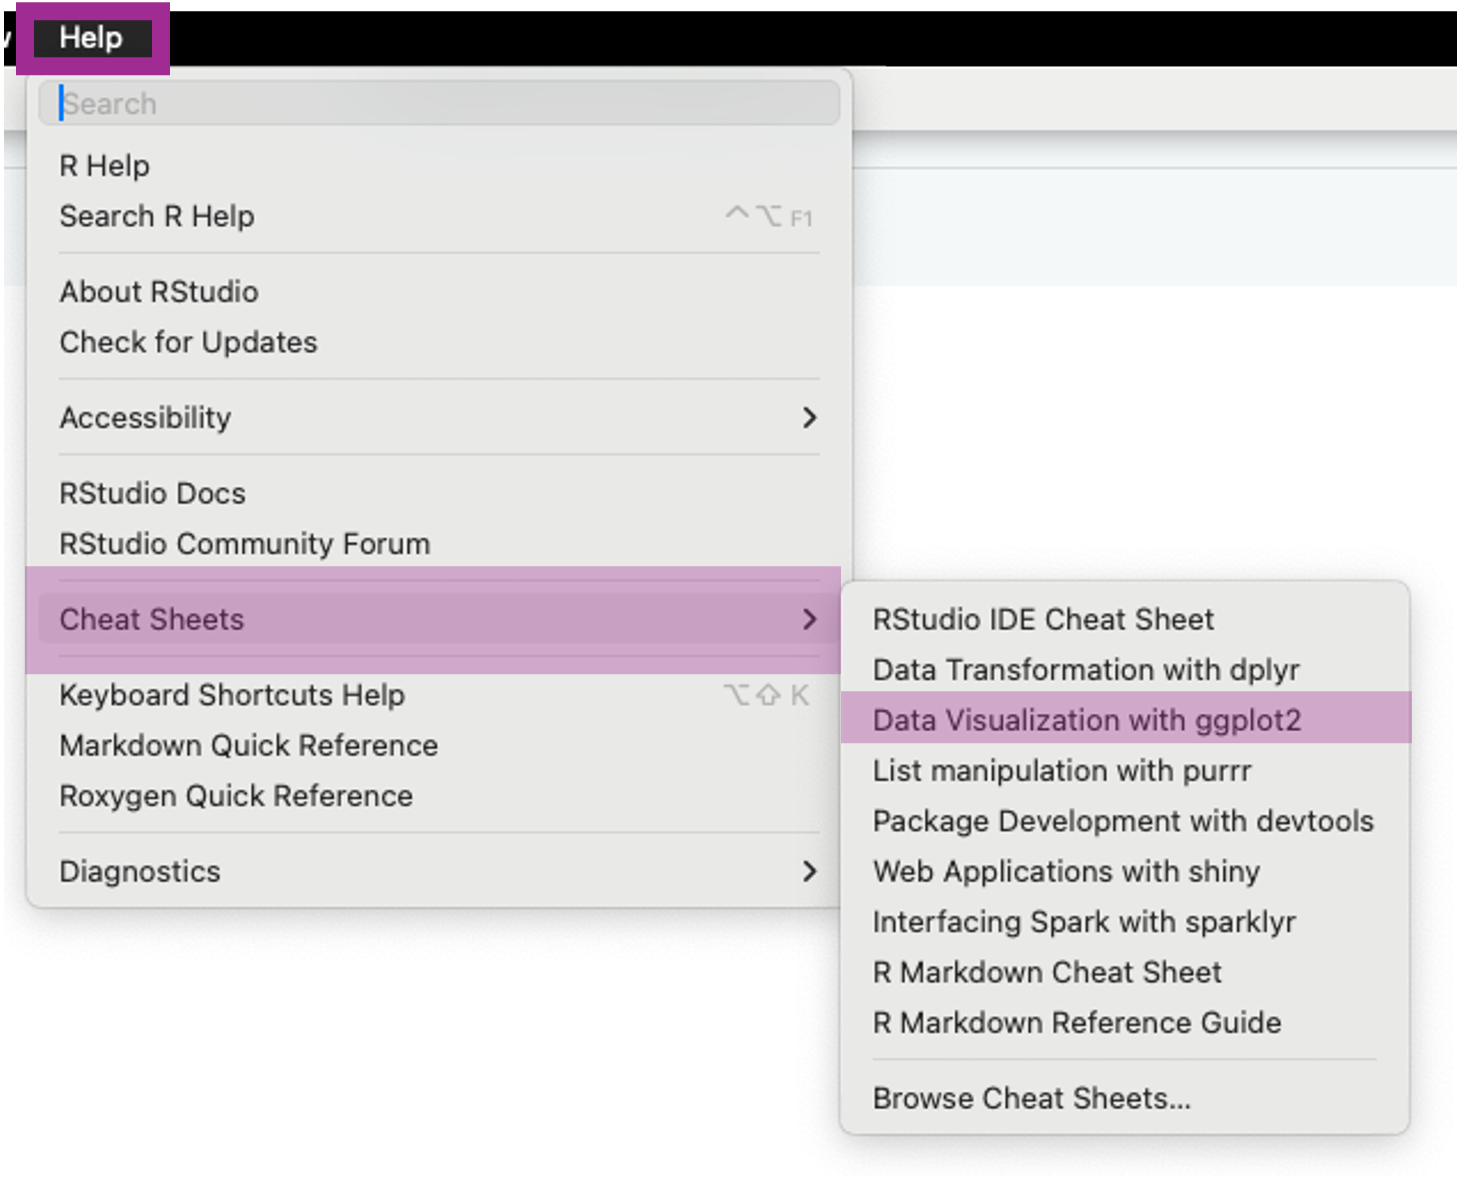
\includegraphics[width=0.5\linewidth]{images/04-ggplotcheatsheet} 

}

\caption{How to access data visualisation cheat sheets in R}\label{fig:cheatSheets}
\end{figure}

As you can see, there are more cheat sheets available within that menu, and even \href{https://posit.co/resources/cheatsheets/?type=posit-cheatsheets/}{more cheat sheets} are available under ``Browse Cheat Sheets\ldots{}''

\subsection{\texorpdfstring{\texttt{help} Function in R}{help Function in R}}\label{sec:RHelp}

To understand how a specific function works, there are two functions you can use: \texttt{help} or \texttt{?}.
This will open some documentation under the \textbf{Help} tab within \textbf{RStudio}. This documentation provides a brief description of the function.
It also includes an example of its use that covers various input arguments, default values for optional arguments, written descriptions of both required and optional arguments, and other relevant information, such as references, similar functions, and worked examples.
Using an example for the function \texttt{sum}, from the base package, which is a function used to add a list of numbers together, the help documentation looks like Figure \ref{fig:example-help}.
To access the help documentation, we have to type \texttt{help(sum)} or \texttt{?sum} into the console and then press enter.

\begin{figure}

{\centering 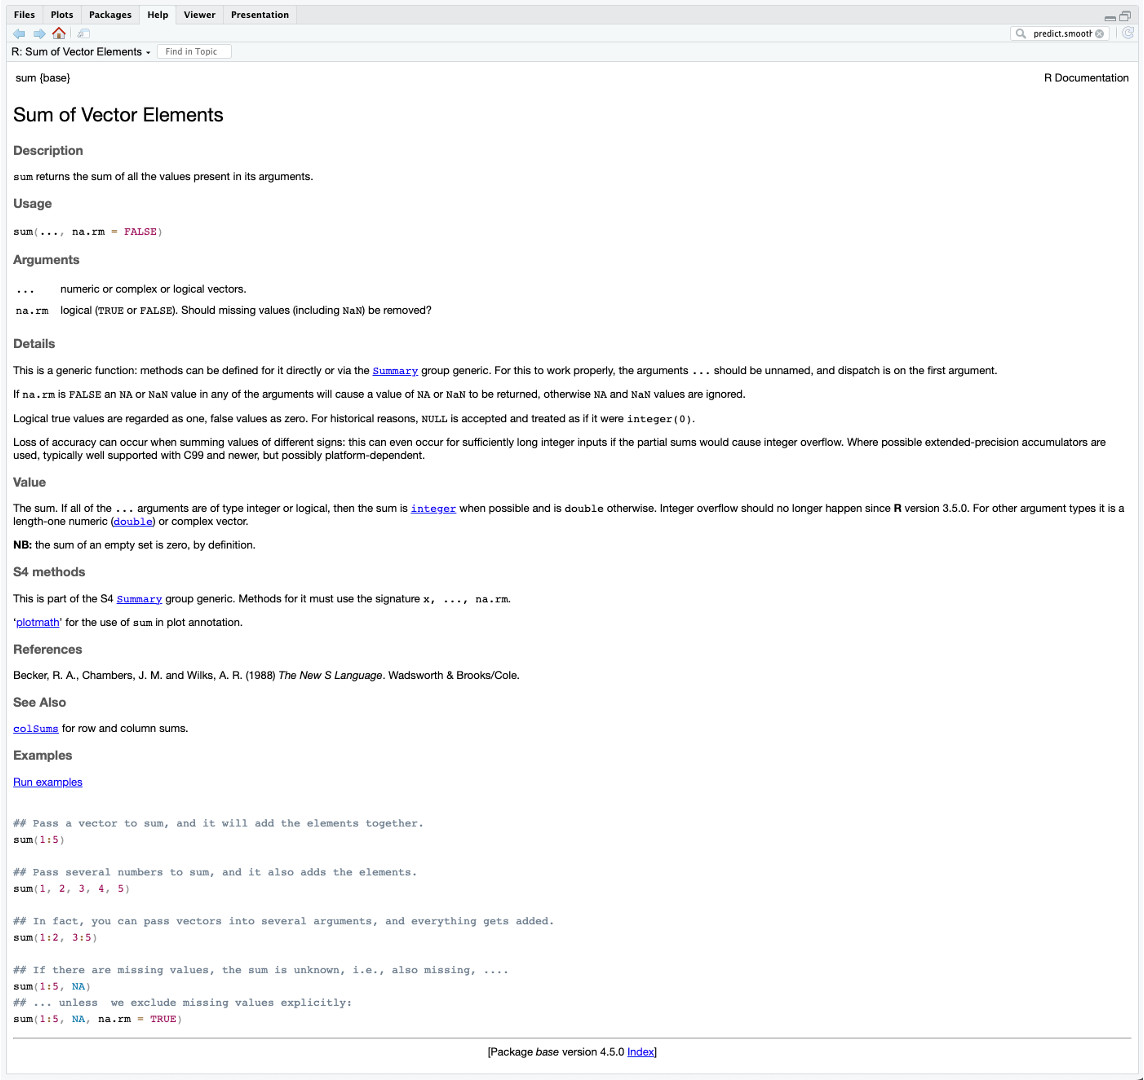
\includegraphics[width=0.95\linewidth]{images/01-help_sum} 

}

\caption{The documentation for `help(sum)` or `?sum`}\label{fig:example-help}
\end{figure}

\subsection{Reference Manuals and Vignettes}\label{sec:RefManAndVignettes}

Many packages have reference manuals which describe each function within the package.
These can be very technical and inaccessible for someone starting out, or trying to understand how to use the functions.
These reference manuals are a compilation of the outputs for \texttt{help} for every function within a package.

\begin{figure}

{\centering 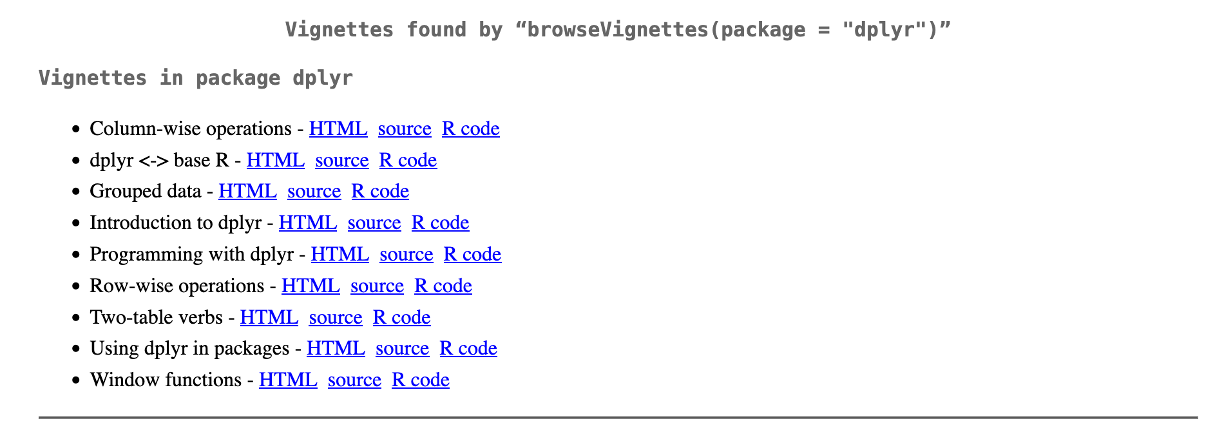
\includegraphics[width=0.8\linewidth]{images/01-dplyr_vignettes} 

}

\caption{The vignettes available for dplyr as shown when using the browseVignettes function}\label{fig:example-vignette}
\end{figure}

Most packages also come with user guides known as vignettes.
Within RStudio, these can be found by typing \texttt{**browseVignettes(package\ =\ "dplyr")**} (using dplyr here as an example package) and then pressing Enter.
This will open a new page on your web browser with links to the vignettes available for the package as seen in Figure \ref{fig:example-vignette}.
Vignettes can also be found on the CRAN page for the package, which is also where the full reference manuals can be found, as seen in Figure \ref{fig:dplyr-CRAN}.

\begin{figure}

{\centering 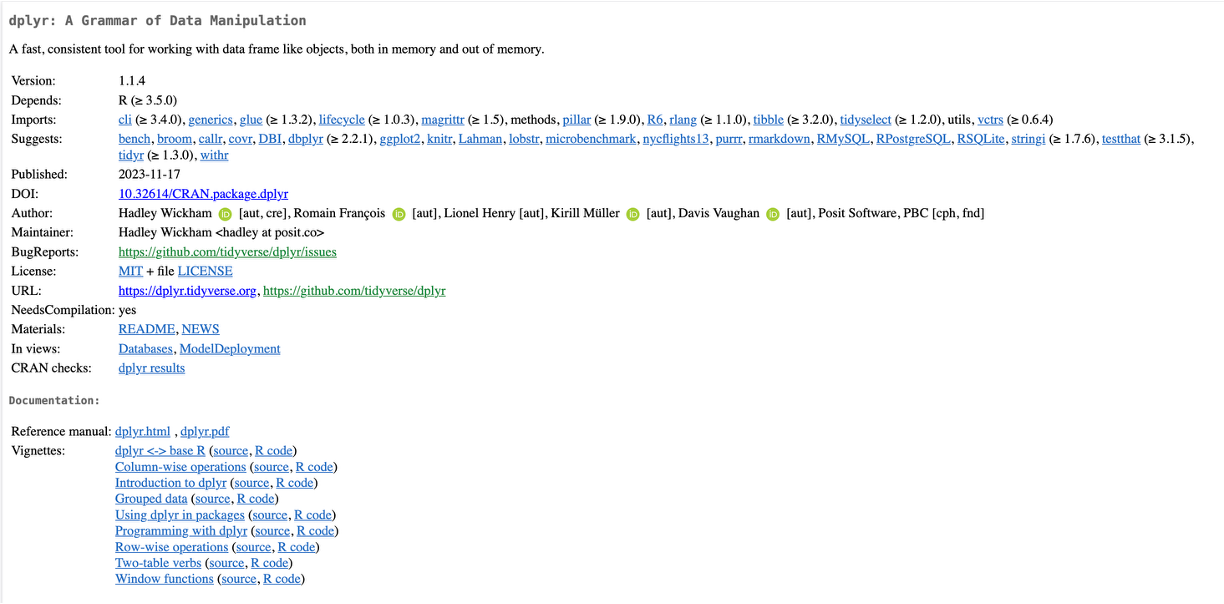
\includegraphics[width=0.8\linewidth]{images/01-dplyr_CRAN} 

}

\caption{The CRAN page for the dplyr package, including urls to the reference manuals and the vignettes}\label{fig:dplyr-CRAN}
\end{figure}

\subsection{Stack Overflow}\label{sec:StackOverflow}

You are very unlikely to come across a problem that is not at least similar to something someone else has encountered, and with the power of the internet, we can be connected to all the people who have tried before us.
\href{https://stackoverflow.com/questions}{Stack Overflow} is a website where people go to ask for help with programming questions.
Often, if you Google a question, a Stack Overflow page will come up as a suggestion, and more often than not, there will be a solution in the answers.
Answers are provided by other users, and up- and down-voted according to how helpful people find them.
\href{https://stackoverflow.com/questions/35090883/remove-all-of-x-axis-labels-in-ggplot/35090981}{An example} of a resolved question in R (that you should be able to answer yourself by the end of this course) is one about removing axis labels from a plot in ggplot2.
The person asking the question provided some simple code that showed the issue without any irrelevant code (called a minimal reproducible example {[}\textbf{\hyperref[acronyms_MRE]{minimal reproducible example (MRE)}}{]} or minimal working example {[}\textbf{\hyperref[acronyms_MWE]{minimal working example (MWE)}}{]}).
Then the person answering gave a very short response, again with a code example, that provides the solution.
Stack Overflow also tends to be very useful when you come across an error you've not encountered before.
For example, \href{https://stackoverflow.com/questions/26247429/data-manipulation-in-r-x-must-be-atomic}{this person} found an error when trying to sort some data, and someone has provided both a solution and an explanation for the error.
Stack Overflow is part of a larger group of websites called the Stack Exchange, which all function in the same way.
Often stats questions can be answered from the \href{https://stats.stackexchange.com/}{stats version} of Stack Overflow.

\subsection{Other}\label{sec:OtherUsefulResources}

There are other sources of information when struggling with a problem in R

\begin{itemize}
\tightlist
\item
  \href{https://www.r-bloggers.com/}{R-bloggers} has blogs dedicated to different topics
\item
  \href{https://github.com/jocelynfriday/UsefulDataSceinceResources}{A selection of useful data science resources} compiled by Jocelyn Friday
\item
  \href{https://www.w3schools.com/r/}{Tutorials} for learning R
\end{itemize}

\chapter{Introduction and basic usage}\label{ch-2}

\section{What are R and RStudio?}\label{what-are-r-and-rstudio}

R is a programming language. Like any language, it gives you the ability to communicate, in this case with your computer. By writing R code, you can give your computer instructions to carry out.

RStudio is an \textbf{\hyperref[acronyms_IDE]{IDE}}. You can use R without RStudio, but RStudio provides a user-friendly method of using R to communicate with your computer. If you want to use R and RStudio on your computer or laptop, you first need to download and install them. You can download R from here: \url{https://cloud.r-project.org/}, and RStudio from here: \url{https://posit.co/download/rstudio-desktop/}. Make sure to select the version that matches your operating system (e.g., Windows, macOS, or Linux) when downloading.

\section{Why use R?}\label{why-use-r}

Many programmes and languages can be used for statistical analysis and data management, but there are several advantages to using and learning R.

While R is not as feature-rich as Python and SAS, it is an all-rounder that can accomplish a wide variety of tasks, e.g., from managing data easily with dplyr and making beautiful graphs with ggplot2, to fitting \emph{P}-splines in generalised additive models using mgcv and causal mediation analysis using CMAverse. If you are analysing big data with a lot of repetition, you can also speed things up with the (relatively) efficient parallel computing with furrr and doParallel (outside the scope of this course). R also has some capabilities as a general programming language, such as managing file systems (e.g., creating, moving, and deleting files). You can also use R to write replicable reports using \textbf{R Markdown} or \textbf{Quarto}, and interactive websites and dashboards using \texttt{shiny}. Lastly, R is free and open source, and it is one of the most widely used languages for statistics and data science. This makes it a valuable skill for careers such as data analyst or data scientist across many fields.

\section{Using R and RStudio}\label{sec:UsingRStudio}

The first time you open RStudio after installing it, it will look like this:

\begin{figure}

{\centering 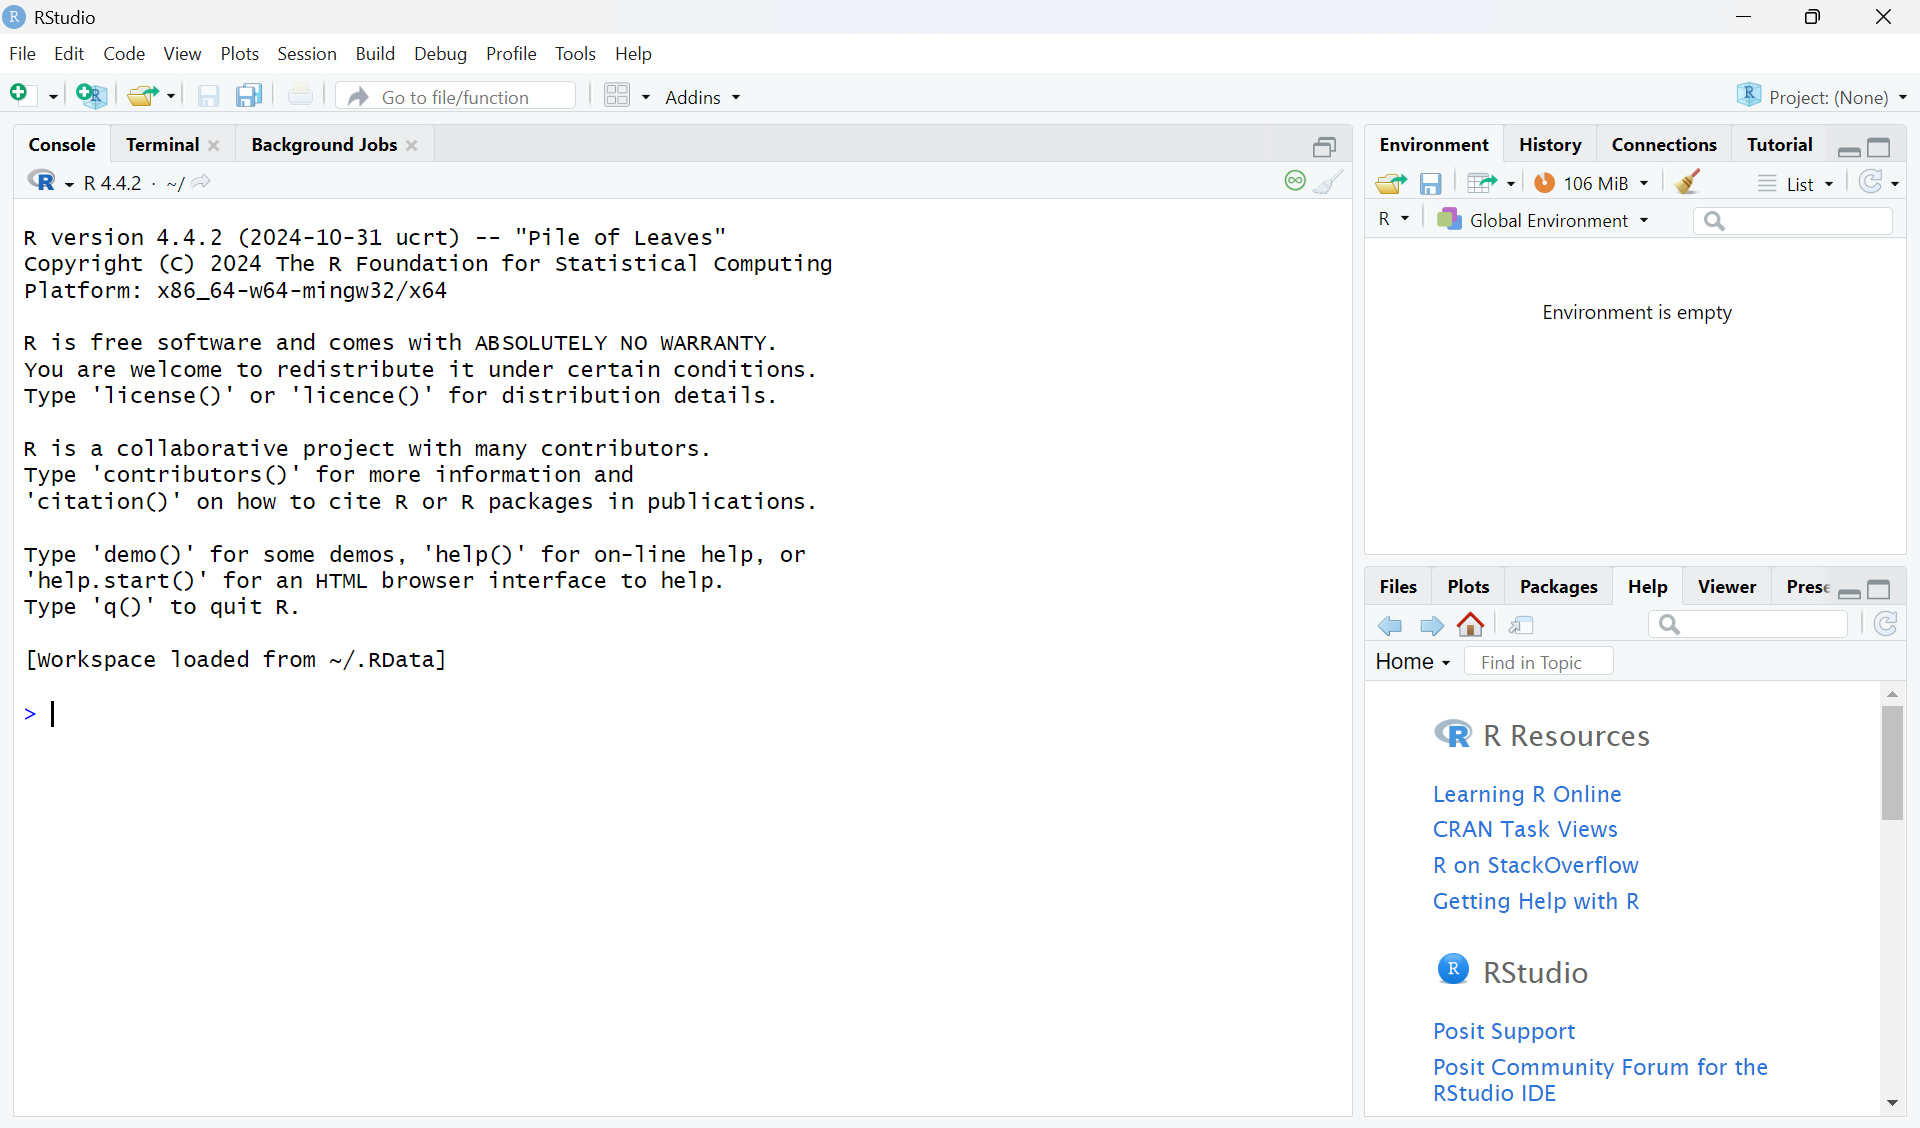
\includegraphics[width=1\linewidth]{images/02-RStudio screenshot - first} 

}

\caption{Home RStudio Screen highlighting the console}\label{fig:home-RStudio-screen}
\end{figure}

The large window on the left is called the \textbf{console} pane. In the console, you can type a command, which will appear next to the blue arrow (\textgreater). If you press Enter, R will execute your command and display the result. Try running the following code and see what happens:

\begin{Shaded}
\begin{Highlighting}[]
\DecValTok{2}\SpecialCharTok{+}\DecValTok{2}
\end{Highlighting}
\end{Shaded}

\begin{verbatim}
## [1] 4
\end{verbatim}

You can also assign a value to a variable, which allows you to reuse the value that is now stored in a. Try typing in your console:

\begin{Shaded}
\begin{Highlighting}[]
\NormalTok{a }\OtherTok{\textless{}{-}} \DecValTok{3}
\end{Highlighting}
\end{Shaded}

Next, look at the Environment pane in the top right. This pane shows you the variables you have created. You should be able to see that the value ``3'' is now associated with your variable ``a''. Try typing in your console:

\begin{Shaded}
\begin{Highlighting}[]
\NormalTok{a}
\end{Highlighting}
\end{Shaded}

\begin{verbatim}
## [1] 3
\end{verbatim}

The console should return ``3'' to you. You could also create a vector of values, and assign this to a variable:

\begin{Shaded}
\begin{Highlighting}[]
\NormalTok{v }\OtherTok{\textless{}{-}} \FunctionTok{c}\NormalTok{(}\DecValTok{1}\NormalTok{, }\DecValTok{5}\NormalTok{, }\DecValTok{8}\NormalTok{)}
\NormalTok{v}
\end{Highlighting}
\end{Shaded}

\begin{verbatim}
## [1] 1 5 8
\end{verbatim}

\section{R scripts}\label{r-scripts}

For simple commands, you can use the console as shown above. However, for more complicated tasks, it will be easier to create an R script. You can create an R script by clicking on File \textgreater{} New File \textgreater{} R Script. This will open an R file in which you can write your code. RStudio should then look like this:

\begin{figure}

{\centering 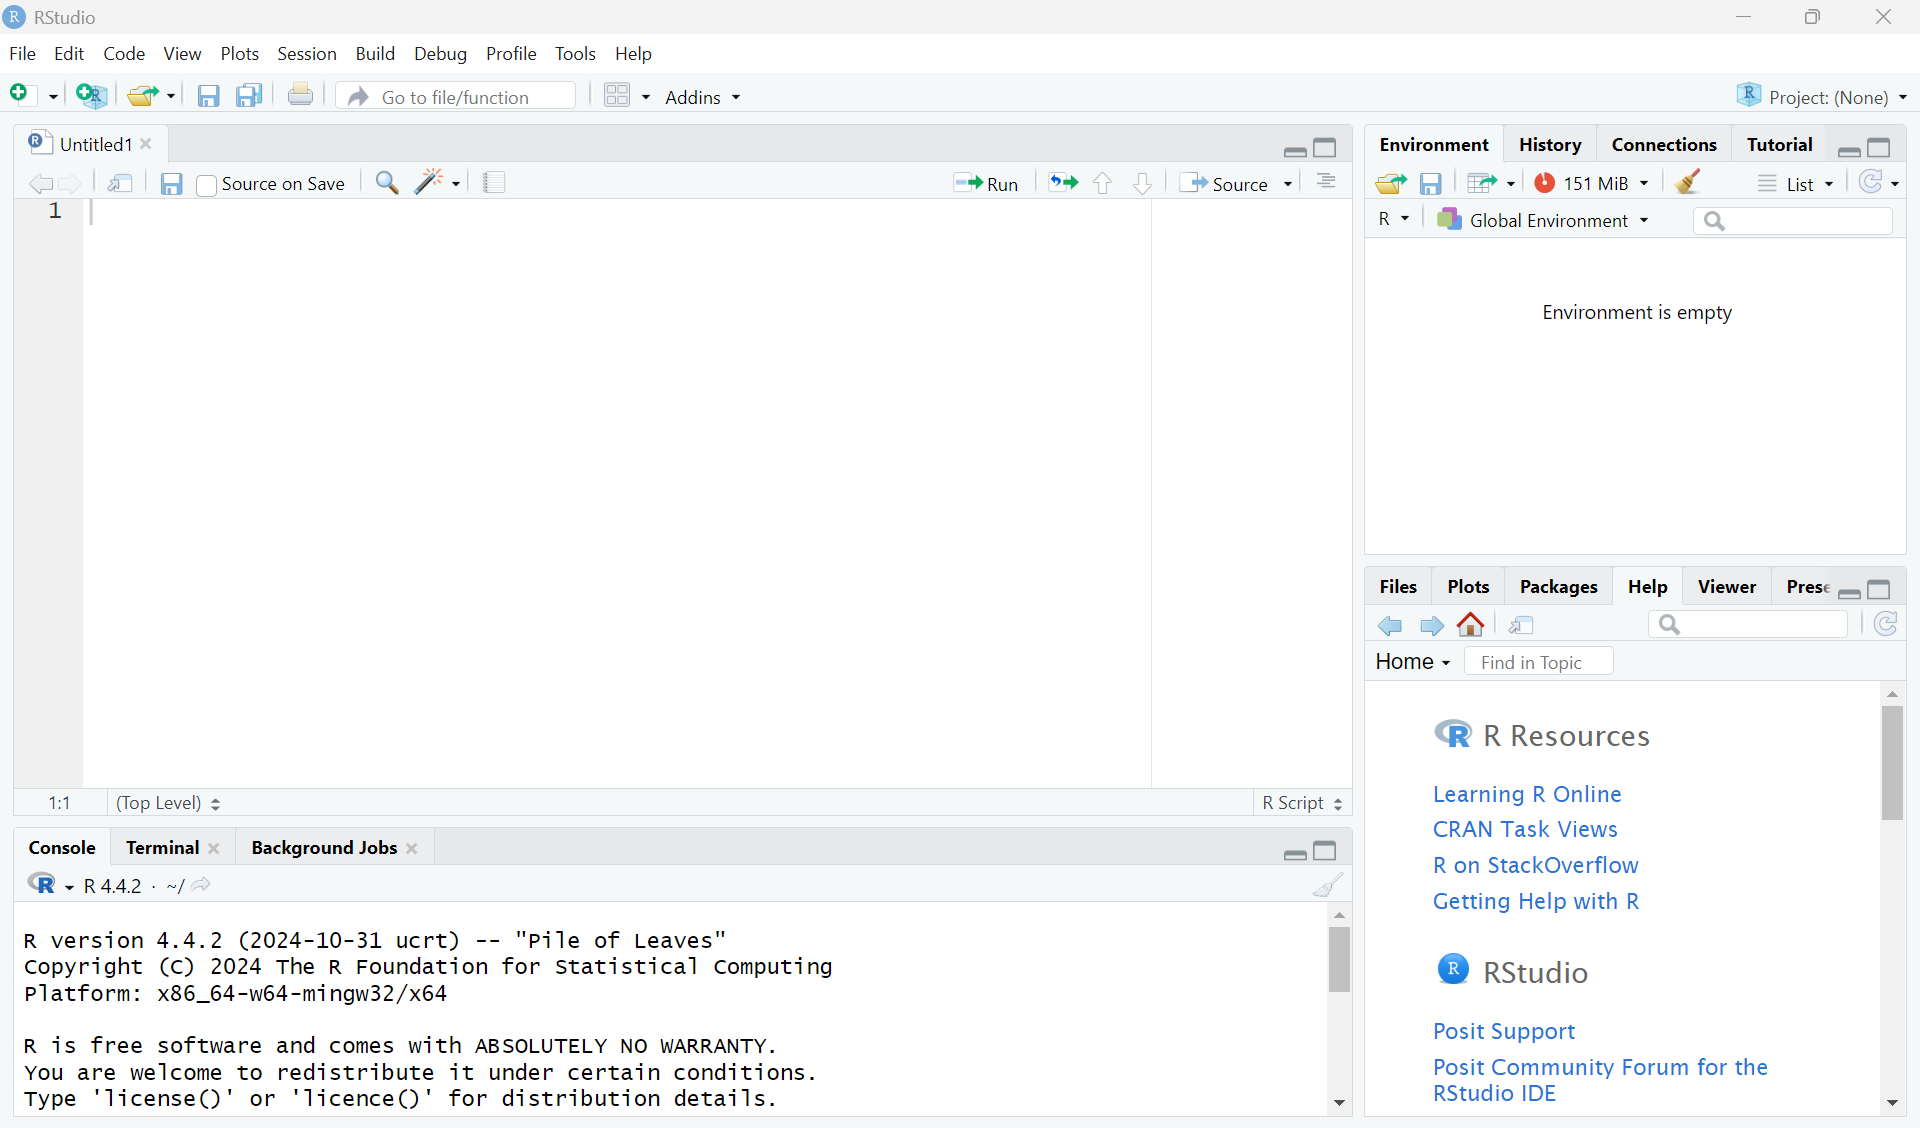
\includegraphics[width=1\linewidth]{images/02-RStudio screenshot} 

}

\caption{Home RStudio Screen highlighting a blank R script}\label{fig:blank-R-script}
\end{figure}

The top left window is the empty script. Add the following code to your R script:

\begin{Shaded}
\begin{Highlighting}[]
\NormalTok{a }\OtherTok{\textless{}{-}} \DecValTok{3}
\NormalTok{b }\OtherTok{\textless{}{-}} \DecValTok{10}
\NormalTok{c }\OtherTok{\textless{}{-}} \DecValTok{5}
\NormalTok{(a}\SpecialCharTok{+}\NormalTok{b)}\SpecialCharTok{*}\NormalTok{c}
\end{Highlighting}
\end{Shaded}

\begin{verbatim}
## [1] 65
\end{verbatim}

The calculation adds two numbers and then multiplies this sum by a third number. You can run the script line by line by pressing the Run button repeatedly. You can also run the entire script by pressing the Source button. You can use the drop-down menu next to the Source button and click on ``Source with Echo'' to ensure your code and its output are printed to the console. Once you have run the script, the Environment pane displays all the variables you created (a, b, c) along with their values.

Once you have created a script, you can save it, so that you can reuse it again later. You can do this by clicking File \textgreater{} Save or File \textgreater{} Save As\ldots{} and specifying a name for your script.

\section{R functions}\label{sec:functions}

If you wanted to do the same calculation multiple times, but for different numbers, you could create something called a function. A function takes an input and uses it to produce an output by using the code defined within the function. Functions can be called multiple times, helping to avoid unnecessary code duplication.

The following code defines the function \textbf{\texttt{sum\_and\_multiply()}}, and calls it with multiple different number combinations as inputs. \textbf{Try it out!}

\begin{Shaded}
\begin{Highlighting}[]
\NormalTok{sum\_and\_multiply }\OtherTok{\textless{}{-}} \ControlFlowTok{function}\NormalTok{(a, b, c) \{}
\NormalTok{  (a}\SpecialCharTok{+}\NormalTok{b)}\SpecialCharTok{*}\NormalTok{c}
\NormalTok{\}}

\FunctionTok{sum\_and\_multiply}\NormalTok{(}\DecValTok{2}\NormalTok{, }\DecValTok{4}\NormalTok{, }\DecValTok{10}\NormalTok{)}
\end{Highlighting}
\end{Shaded}

\begin{verbatim}
## [1] 60
\end{verbatim}

\begin{Shaded}
\begin{Highlighting}[]
\FunctionTok{sum\_and\_multiply}\NormalTok{(}\DecValTok{6}\NormalTok{, }\DecValTok{8}\NormalTok{, }\DecValTok{2}\NormalTok{)}
\end{Highlighting}
\end{Shaded}

\begin{verbatim}
## [1] 28
\end{verbatim}

\begin{Shaded}
\begin{Highlighting}[]
\FunctionTok{sum\_and\_multiply}\NormalTok{(}\DecValTok{1}\NormalTok{, }\DecValTok{5}\NormalTok{, }\DecValTok{2}\NormalTok{)}
\end{Highlighting}
\end{Shaded}

\begin{verbatim}
## [1] 12
\end{verbatim}

Now try writing your own function!

What if you now wanted to calculate the mean and the \textbf{\hyperref[acronyms_SD]{standard deviation (SD)}} of a series of numbers? You could again write your own function. Alternatively, you can use existing functions. R has a large number of built-in functions that are ready to use. The functions \textbf{\texttt{mean()}} and \textbf{\texttt{sd()}} can be used to calculate the mean and standard deviation, respectively. You can use the \textbf{\texttt{help()}} function or place a ``?'' in front of your function. This will provide access to the documentation pages of that function and provide guidance on how to use it.

Try this:

\begin{Shaded}
\begin{Highlighting}[]
\NormalTok{utils}\SpecialCharTok{::}\FunctionTok{help}\NormalTok{(mean)}
\end{Highlighting}
\end{Shaded}

and this:

\begin{Shaded}
\begin{Highlighting}[]
\NormalTok{?sd}
\end{Highlighting}
\end{Shaded}

The documentation should have appeared in the bottom-right corner of RStudio. Did the documentation give enough information to use these two functions?

Here is one way in which you can calculate the mean and standard deviation of a series of numbers:

\begin{Shaded}
\begin{Highlighting}[]
\NormalTok{x }\OtherTok{\textless{}{-}} \FunctionTok{c}\NormalTok{(}\DecValTok{1}\NormalTok{, }\DecValTok{4}\NormalTok{, }\DecValTok{7}\NormalTok{, }\DecValTok{3}\NormalTok{)}
\NormalTok{base}\SpecialCharTok{::}\FunctionTok{mean}\NormalTok{(x)}
\end{Highlighting}
\end{Shaded}

\begin{verbatim}
## [1] 3.75
\end{verbatim}

\begin{Shaded}
\begin{Highlighting}[]
\NormalTok{stats}\SpecialCharTok{::}\FunctionTok{sd}\NormalTok{(x)}
\end{Highlighting}
\end{Shaded}

\begin{verbatim}
## [1] 2.5
\end{verbatim}

\section{Environment and scope}\label{sec:scope}

The above examples have shown how to create and save data in R. By default, these data are stored in the \textbf{global environment}, which is accessible to all functions in R. However, variables created inside a function are generally only available within that function's scope and are not accessible to other functions. Below is an example of calculating the area of a right-angled triangle:

\begin{Shaded}
\begin{Highlighting}[]
\NormalTok{area }\OtherTok{\textless{}{-}} \ControlFlowTok{function}\NormalTok{(base, hypotenuse)\{}
\NormalTok{  x }\OtherTok{\textless{}{-}}\NormalTok{ base }\SpecialCharTok{*}\NormalTok{ hypotenuse}
  \FunctionTok{return}\NormalTok{(x }\SpecialCharTok{/} \DecValTok{2}\NormalTok{)}
\NormalTok{\}}

\FunctionTok{area}\NormalTok{(}\DecValTok{3}\NormalTok{, }\DecValTok{2}\NormalTok{)}
\end{Highlighting}
\end{Shaded}

\begin{verbatim}
## [1] 3
\end{verbatim}

\begin{Shaded}
\begin{Highlighting}[]
\NormalTok{x}
\end{Highlighting}
\end{Shaded}

\begin{verbatim}
## [1] 1 4 7 3
\end{verbatim}

Note: even though we have run the \textbf{\texttt{area()}} function, we can't recall the value of x (which is defined and calculated inside that \textbf{\texttt{area()}} function. This is because the value of x was not saved in the global environment and is gone as long as the function call is finished. This concept is not necessary to understand to use R, however it is useful for anyone who may use functions in the future.

\section{Packages}\label{packages}

Base R encompasses all the functions and features included with R upon installation. The double-colon operator `::' tells R to select definitions from the named package on the right. For example, mean and sd are examples of base R functions. Other R users have created their own functions and shared them online as installable packages, enabling others to use them for free. These are not part of base R and, therefore, need to be installed separately. Most R packages can be found on CRAN (\url{https://cran.r-project.org/}). To install a package from CRAN, you can use the install.packages function. Let's say you wish to now calculate the \textbf{\hyperref[acronyms_SE]{standard error (SE)}} of a series of numbers. You can calculate this by using a formula, but you can also use an already existing function. The package plotrix contains the function std.error, which can calculate this. plotrix is not part of base R, so needs to be installed.

Try:

\begin{Shaded}
\begin{Highlighting}[]
\NormalTok{utils}\SpecialCharTok{::}\FunctionTok{install.packages}\NormalTok{(}\StringTok{"plotrix"}\NormalTok{)}
\end{Highlighting}
\end{Shaded}

To use a package you installed, you first need to load it with the \texttt{library()} function. You should then be able to use the std.error function:

\begin{Shaded}
\begin{Highlighting}[]
\NormalTok{base}\SpecialCharTok{::}\FunctionTok{library}\NormalTok{(plotrix)}

\NormalTok{plotrix}\SpecialCharTok{::}\FunctionTok{std.error}\NormalTok{(x)}
\end{Highlighting}
\end{Shaded}

\begin{verbatim}
## [1] 1.25
\end{verbatim}

Can you find a different function that is not part of base R, install the relevant package, and use it?

\section{Reserved words}\label{sec:reservedWords}

R has reserved words that have a special meaning within the language. You cannot use them as a function or a variable name. To find out what the reserved words are, you can type:

\begin{Shaded}
\begin{Highlighting}[]
\NormalTok{?reserved}
\end{Highlighting}
\end{Shaded}

From the list, you can see that ``if'' and ``else'' are reserved words. Try writing:

\begin{Shaded}
\begin{Highlighting}[]
\ControlFlowTok{if} \OtherTok{\textless{}{-}} \DecValTok{3}
\end{Highlighting}
\end{Shaded}

\begin{verbatim}
## Error in parse(text = input): <text>:1:4: unexpected assignment
## 1: if <-
##        ^
\end{verbatim}

As expected, the R console will print an error, and will not have assigned the value ``3'' to ``if''. R is case sensitive. This means that it distinguishes between if, If, iF, and IF. This means that you would be able to assign a value to If, iF, or IF. Try it:

\begin{Shaded}
\begin{Highlighting}[]
\NormalTok{If }\OtherTok{\textless{}{-}} \DecValTok{3}
\end{Highlighting}
\end{Shaded}

Now, the value of ``3'' should be assigned to If.

\section{Error vs warning messages}\label{sec:ErrorVsWarning}

In the previous section, the R console printed an error message and did not run the code. Running R code can also generate warning messages. The code will still run, but may not behave as expected. Here is an example of that code that runs, but will generate a warning message:

\begin{Shaded}
\begin{Highlighting}[]
\NormalTok{v }\OtherTok{\textless{}{-}} \FunctionTok{c}\NormalTok{(}\StringTok{"1"}\NormalTok{, }\StringTok{"2"}\NormalTok{, }\StringTok{"3"}\NormalTok{)}
\NormalTok{base}\SpecialCharTok{::}\FunctionTok{mean}\NormalTok{(v)}
\end{Highlighting}
\end{Shaded}

\begin{verbatim}
## Warning in mean.default(v): argument is not numeric or logical: returning NA
\end{verbatim}

\begin{verbatim}
## [1] NA
\end{verbatim}

You may expect the output of the above code to be 2. However, the function mean expects its input to be a vector of numbers, not strings. Therefore, the code produces a warning message, and \textbf{\hyperref[acronyms_NA]{not available (NA)}} as the output.

\section{Working directory}\label{sec:WorkingDirectory}

R allows you to read files from your computer and save files to it. How does R know where to read from or save to? You can provide a full file path. If no full path is provided, R assumes the file is located in the working directory. The working directory is the default location on your computer where R reads and saves files. To find out what your working directory is, type \texttt{getwd()}:

\begin{Shaded}
\begin{Highlighting}[]
\FunctionTok{getwd}\NormalTok{()}
\end{Highlighting}
\end{Shaded}

\begin{verbatim}
## [1] "C:/Users/cresc/OneDrive - University of Glasgow/Teaching/MED5686 - R for Health Data Science/R4HDS_bookdown"
\end{verbatim}

Are you happy with that working directory? If not, you can change it using \texttt{setwd()}:

\begin{Shaded}
\begin{Highlighting}[]
\FunctionTok{setwd}\NormalTok{(}\StringTok{\textquotesingle{}path\textquotesingle{}}\NormalTok{)}
\end{Highlighting}
\end{Shaded}

To demonstrate the working directory, you can create a simple text file called ``R output.txt'' by using the command \texttt{writeLines()}. Please note that the command will overwrite any existing text file with the same name.

\begin{Shaded}
\begin{Highlighting}[]
\NormalTok{base}\SpecialCharTok{::}\FunctionTok{writeLines}\NormalTok{(}\StringTok{"Hello World"}\NormalTok{, }\StringTok{"R output.txt"}\NormalTok{)}
\end{Highlighting}
\end{Shaded}

Open your file explorer and navigate to your working directory. You should be able to find the file \texttt{R\ output.txt}, with the line \texttt{Hello\ World} within it.

Please note: you can also set your working directory by clicking Session \textgreater{} Set Working Directory \textgreater{} Choose Directory (or source file location).

\section{Import data}\label{import-data}

The examples above used data that were input directly into R's console. However, real-world data analysis typically utilises data stored in files on either local or network drives. In those scenarios, you will need to import the data from the files into R. The exact functions used to import data depend on the data format. One of the most common formats of data is a \textbf{\hyperref[acronyms_CSV]{comma separated value (CSV)}} file, and we will use that as an example. Please download \textbf{02-hrqol\_data.csv} from Moodle, and place it in a convenient folder. For example, if you have put the data file in \textbf{\texttt{C:/Users/ABC/R\_course/Data}}, then you can import the data using \texttt{read.csv()}:

\begin{Shaded}
\begin{Highlighting}[]
\NormalTok{dat }\OtherTok{\textless{}{-}}\NormalTok{ utils}\SpecialCharTok{::}\FunctionTok{read.csv}\NormalTok{(}\StringTok{"./data/02{-}hrqol\_data.csv"}\NormalTok{)}
\end{Highlighting}
\end{Shaded}

Note that the code not only imports the data, but also stores the imported data in a data frame object called \textbf{\texttt{dat}} (see Section \ref{sec:dataFrame}). It is common practice to store the imported data in an object, because without doing so, you cannot interact with the data after loading it.

Below is a table showing common data formats and some functions to import them:

\begin{table}

\caption{\label{tab:data-import}Functions to import data into R}
\centering
\begin{tabular}[t]{l|l|l}
\hline
File format (file name extension) & base R & Using additional packages\\
\hline
CSV (.csv) & read.csv & read\_csv\\
\hline
TSV (.tsv) & read.table & read\_tsv\\
\hline
TXT (.txt) & read.delim & read\_delim\\
\hline
Excel data file (.xlsx / .xls) &  & read\_excel\\
\hline
STATA data file (.dta) &  & read\_dta\\
\hline
SPSS data file (.sav) &  & read\_sav\\
\hline
SAS data file (.sas7bdat) &  & read\_sas\\
\hline
\end{tabular}
\end{table}

If you haven't installed those additional packages (readr, readxl, haven), the code on the right column won't work. You must install the package as described in the above section before running the code. Also note that the readr in the read\_csv command means that the read\_csv function is in the readr package specifically.

\section{Export data}\label{export-data}

If you have made changes to the data in R and want to export a copy to a local or network drive. You can export data in a similar way with \texttt{write.csv()}:

\begin{Shaded}
\begin{Highlighting}[]
\NormalTok{utils}\SpecialCharTok{::}\FunctionTok{write.csv}\NormalTok{(dat }\SpecialCharTok{*} \DecValTok{2}\NormalTok{, }\StringTok{\textquotesingle{}C:/Users/ABC/R\_course/Data/test\_data\_new.csv\textquotesingle{}}\NormalTok{)}
\end{Highlighting}
\end{Shaded}

As with data import, R can export data in various formats using different packages.The corresponding functions are listed in the table below:

\begin{table}

\caption{\label{tab:data-export}Functions to export data from R}
\centering
\begin{tabular}[t]{l|l|l}
\hline
File format (file name extension) & Base R & Using additional packages\\
\hline
CSV (.csv) & write.csv & write\_csv\\
\hline
TSV (.tsv) & write.table & write\_tsv\\
\hline
TXT (.txt) & writeLines & write\_delim\\
\hline
Excel data file (.xlsx) &  & write\_xlsx\\
\hline
STATA data file (.dta) &  & write\_dta\\
\hline
SPSS data file (.sav) &  & write\_sav\\
\hline
SAS data file (.sas7bdat) &  & write\_sas\\
\hline
\end{tabular}
\end{table}

Be aware that some data formats may not correspond to the standard extension. For example, a data formatted as \textbf{\hyperref[acronyms_TSV]{tab separated value (TSV)}} could have an extension of `.txt'. If the imported data doesn't make sense (e.g., only one column), please review the imported data and determine if a different function should be used instead. Also note that the Excel data requires a different package for export than it did for import (writexl).

\section{Project}\label{sec:project}

The \textbf{Project} functionality in R is a good way to manage different projects. For example, you can use one project for all scripts for this course and another project for your \textbf{\hyperref[acronyms_MPH]{Master's of Public Health (MPH)}} project (if you decide to use R for it).

The main advantage of using the \textbf{project} functionality is that the \textbf{working directory} is set automatically to your project folder, and it could be easier to import data or scripts into R without using absolute paths. For example, if you have a project folder \textbf{\texttt{"C:/Users/ABC/R\_course/"}} for this course, and the data `02-hrqol\_data.csv' located in the \textbf{\texttt{"C:/Users/ABC/R\_course/Data/02-hrqol\_data.csv"}}, you can either read in the data using an absolute path:

\begin{Shaded}
\begin{Highlighting}[]
\NormalTok{dat }\OtherTok{\textless{}{-}} \FunctionTok{read.csv}\NormalTok{(}\StringTok{"C:/Users/ABC/R\_course/data/02{-}hrqol\_data.csv"}\NormalTok{)}
\end{Highlighting}
\end{Shaded}

Or using a relative path, if your working directory is set correctly (or if you use the Project function):

\begin{Shaded}
\begin{Highlighting}[]
\NormalTok{dat }\OtherTok{\textless{}{-}} \FunctionTok{read.csv}\NormalTok{(}\StringTok{"data/02{-}hrqol\_data.csv"}\NormalTok{)}
\end{Highlighting}
\end{Shaded}

Similarly, you can use a relative path when you export files.

To create an R Project, you can click on the project button in the top-right corner of your RStudio.

\begin{figure}

{\centering 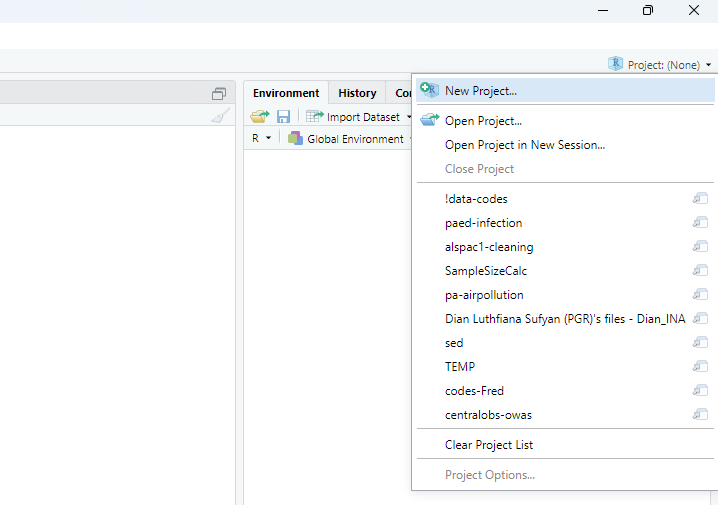
\includegraphics[width=0.75\linewidth]{images/02-R_project_1} 

}

\caption{Project Menu in RStudio}\label{fig:project-menu}
\end{figure}

You then can create a project by clicking the \textbf{New Project\ldots{}} button, which then gives you an option to create a new project by creating a new folder (which would be empty) or to create a new project based on an existing folder (where there may already be data and other relevant files in it). In Figure \ref{fig:project-menu}, you can also see that all recent projects that you have used are listed there, which could be handy to switch between ongoing projects.

\begin{figure}

{\centering 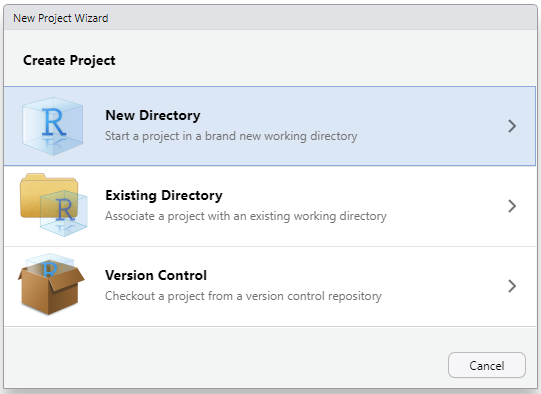
\includegraphics[width=0.75\linewidth]{images/02-R_project_2} 

}

\caption{Options to create a new project}\label{fig:new-project-wizard}
\end{figure}

\section{R Markdown}\label{sec:RMarkdown}

R Markdown enables you to combine code, code output, images, and plain text into one document (Word, \textbf{\hyperref[acronyms_PDF]{portable document format (PDF)}} or \textbf{\hyperref[acronyms_HTML]{hypertext markup language (HTML)}}). R Markdown lets you directly produce a nicely formatted report, without needing to copy and paste the results of your analysis into a separate document.

Using R Markdown can be more efficient, transparent, and supports the reproducibility of your work. To use R Markdown you first need to install the rmarkdown package.

\begin{Shaded}
\begin{Highlighting}[]
\FunctionTok{install.packages}\NormalTok{(}\StringTok{\textquotesingle{}rmarkdown\textquotesingle{}}\NormalTok{)}
\end{Highlighting}
\end{Shaded}

If you would like to create a \textbf{\hyperref[acronyms_PDF]{PDF}} or Word document using R Markdown, you will also need to have a version of LaTeX installed on your computer. If you do not yet have a version of LaTeX installed on your computer, tinytex (\url{https://yihui.org/tinytex/}) is a good choice. You can install rmarkdown and tinytex with the following commands:

\begin{Shaded}
\begin{Highlighting}[]
\NormalTok{utils}\SpecialCharTok{::}\FunctionTok{install.packages}\NormalTok{(}\StringTok{\textquotesingle{}tinytex\textquotesingle{}}\NormalTok{)}
\NormalTok{tinytex}\SpecialCharTok{::}\FunctionTok{install\_tinytex}\NormalTok{()}
\end{Highlighting}
\end{Shaded}

You can create an R Markdown document by clicking New File \textgreater{} R Markdown\ldots{} Give the document a title and add your name in the `Author box', and click on `OK'. This will create an R Markdown file. Save this file in your working directory. You can now knit it by clicking on the `Knit' button. Wait for it to finish and have a look at the output.

You can also run the code sections (``chunks'') without `knitting' the document by pressing the green arrow in each chunk. Have a look at the Run drop-down menu for other Run options.

Try adding some code and text of your own to your R Markdown file, run your code chunks, and knit the file to get a feel for how it works.

\section{R coding tips}\label{sec:CodingTips}

The above examples are relatively simple. However, if you start writing more complicated and larger pieces of code, consistently formatting your code will help its readability, maintainability, and help you spot errors. Below are some tips for writing your R code.

\subsection{Indentation}\label{indentation}

Compare these two code snippets:

\begin{Shaded}
\begin{Highlighting}[]
\NormalTok{x }\OtherTok{\textless{}{-}} \DecValTok{3}

\ControlFlowTok{if}\NormalTok{(x }\SpecialCharTok{\%\%} \DecValTok{2} \SpecialCharTok{==} \DecValTok{0}\NormalTok{) \{}
\NormalTok{base}\SpecialCharTok{::}\FunctionTok{print}\NormalTok{(}\StringTok{"Even number"}\NormalTok{)}
\NormalTok{\} }\ControlFlowTok{else} \ControlFlowTok{if}\NormalTok{ (x }\SpecialCharTok{\%\%} \DecValTok{2} \SpecialCharTok{==} \DecValTok{1}\NormalTok{) \{}
\NormalTok{base}\SpecialCharTok{::}\FunctionTok{print}\NormalTok{(}\StringTok{"Odd number"}\NormalTok{)}
\NormalTok{\} }\ControlFlowTok{else}
\NormalTok{base}\SpecialCharTok{::}\FunctionTok{print}\NormalTok{(}\StringTok{"Number is neither even nor odd"}\NormalTok{)}
\end{Highlighting}
\end{Shaded}

\begin{verbatim}
## [1] "Odd number"
\end{verbatim}

\begin{Shaded}
\begin{Highlighting}[]
\ControlFlowTok{if}\NormalTok{(x }\SpecialCharTok{\%\%} \DecValTok{2} \SpecialCharTok{==} \DecValTok{0}\NormalTok{) \{}
\NormalTok{  base}\SpecialCharTok{::}\FunctionTok{print}\NormalTok{(}\StringTok{"Even number"}\NormalTok{)}
\NormalTok{\} }\ControlFlowTok{else} \ControlFlowTok{if}\NormalTok{ (x }\SpecialCharTok{\%\%} \DecValTok{2} \SpecialCharTok{==} \DecValTok{1}\NormalTok{) \{}
\NormalTok{  base}\SpecialCharTok{::}\FunctionTok{print}\NormalTok{(}\StringTok{"Odd number"}\NormalTok{)}
\NormalTok{\} }\ControlFlowTok{else}
\NormalTok{  base}\SpecialCharTok{::}\FunctionTok{print}\NormalTok{(}\StringTok{"Number is neither even nor odd"}\NormalTok{)}
\end{Highlighting}
\end{Shaded}

\begin{verbatim}
## [1] "Odd number"
\end{verbatim}

The first code snippet does not use indentation (spaces at the beginning of a line of code), while the second does. Consistent use of indentation can aid readability.

\subsection{Commenting}\label{commenting}

For the code above, you may have inferred that it tells you whether a number is even or odd (or neither). However, you may not understand how it does that. Adding comments to your code can help explain to others how it works. It will also help you to understand your own code if you need to use or edit it in the future. You can add comments by using the ``\#'' symbol. See below how the added comments help to clarify what the code does and how it accomplishes this.

\begin{Shaded}
\begin{Highlighting}[]
\CommentTok{\# the following code determines whether a number is even, odd, or neither}
\CommentTok{\# it does this by using the modulo (\%\%) operator}
\CommentTok{\# the modulo operator returns the remainder of a division}
\CommentTok{\# the remainder of an even number divided by 2 is 0}
\CommentTok{\# the remainder of an odd number divided by 2 is 1}
\CommentTok{\# the remainder of a decimal number divided by 2 is always another decimal number}
\CommentTok{\# therefore, for a decimal number, the else condition would hold}

\ControlFlowTok{if}\NormalTok{(x }\SpecialCharTok{\%\%} \DecValTok{2} \SpecialCharTok{==} \DecValTok{0}\NormalTok{) \{}
\NormalTok{  base}\SpecialCharTok{::}\FunctionTok{print}\NormalTok{(}\StringTok{"Even number"}\NormalTok{)}
\NormalTok{\} }\ControlFlowTok{else} \ControlFlowTok{if}\NormalTok{ (x }\SpecialCharTok{\%\%} \DecValTok{2} \SpecialCharTok{==} \DecValTok{1}\NormalTok{) \{}
\NormalTok{  base}\SpecialCharTok{::}\FunctionTok{print}\NormalTok{(}\StringTok{"Odd number"}\NormalTok{)}
\NormalTok{\} }\ControlFlowTok{else}
\NormalTok{  base}\SpecialCharTok{::}\FunctionTok{print}\NormalTok{(}\StringTok{"Number is neither even nor odd"}\NormalTok{)}
\end{Highlighting}
\end{Shaded}

\begin{verbatim}
## [1] "Odd number"
\end{verbatim}

Try adding relevant comments to the function you wrote previously.

\subsection{Naming conventions}\label{sec:NamingConventions}

Being consistent with how you name your variables and functions can further improve your code's readability. Try to choose names that are short and meaningful.

\begin{Shaded}
\begin{Highlighting}[]
\CommentTok{\# short, but not informative}
\NormalTok{x }\OtherTok{\textless{}{-}} \StringTok{"December"}

\CommentTok{\# informative, but long}
\NormalTok{twelfth\_month\_of\_the\_year }\OtherTok{\textless{}{-}} \StringTok{"December"}

\CommentTok{\# both short and informative}
\NormalTok{month\_12 }\OtherTok{\textless{}{-}} \StringTok{"December"}
\end{Highlighting}
\end{Shaded}

Did the function you wrote previously have a short and meaningful name? If not, change it.

It is also best not to reuse existing function names. Reusing a function name will overwrite the original function. Here is an example:

\begin{Shaded}
\begin{Highlighting}[]
\NormalTok{c }\OtherTok{\textless{}{-}} \ControlFlowTok{function}\NormalTok{(a, b, c) \{}
\NormalTok{  (a}\SpecialCharTok{+}\NormalTok{b)}\SpecialCharTok{*}\NormalTok{c}
\NormalTok{\}}
\end{Highlighting}
\end{Shaded}

The above code will overwrite the base R function c, which combines values into a vector (this will be covered further in Section \ref{sec:vector}). If you were to use c again, it would refer to the function in the above yellow box.

\subsection{Style guides}\label{sec:styleGuides}

The above sections provide a few tips on how to improve the readability of your code. For further ideas/guidance on how to write and format your code, you can refer to a style guide. Here is an example of a style guide: \href{https://style.tidyverse.org/}{Tidyverse Style Guide}. Have a look!

\section{References/further reading}\label{referencesfurther-reading}

\begin{enumerate}
\def\labelenumi{\arabic{enumi}.}
\tightlist
\item
  \url{https://rstudio-education.github.io/hopr/}
\item
  \url{https://intro2r.com/}
\item
  \url{https://docs.posit.co/ide/user/}
\end{enumerate}

\chapter{Data Types \& Manipulation}\label{ch-3}

\begin{verbatim}
## -- Attaching core tidyverse packages ------------------------ tidyverse 2.0.0 --
## v dplyr     1.1.4     v readr     2.1.6
## v forcats   1.0.1     v stringr   1.6.0
## v ggplot2   4.0.2     v tibble    3.3.1
## v lubridate 1.9.4     v tidyr     1.3.2
## v purrr     1.2.1     
## -- Conflicts ------------------------------------------ tidyverse_conflicts() --
## x dplyr::filter() masks stats::filter()
## x dplyr::lag()    masks stats::lag()
## i Use the conflicted package (<http://conflicted.r-lib.org/>) to force all conflicts to become errors
## 
## Attaching package: 'hms'
## 
## 
## The following object is masked from 'package:lubridate':
## 
##     hms
\end{verbatim}

\begin{verbatim}
##           used  (Mb) gc trigger  (Mb) max used  (Mb)
## Ncells 2279404 121.8    4157530 222.1  4157530 222.1
## Vcells 4002148  30.6    8388608  64.0  6671981  51.0
\end{verbatim}

At the heart of almost all of R, nearly everything in R is an \textbf{object} of some form or fashion. These can be almost anything, from a single number or word to more complex things such as functions (as seen in Section \ref{sec:functions}), data sets, plots (coming in Chapter \ref{ch-4}), and analysis results (coming in Chapter \ref{ch-5}).

\begin{figure}

{\centering 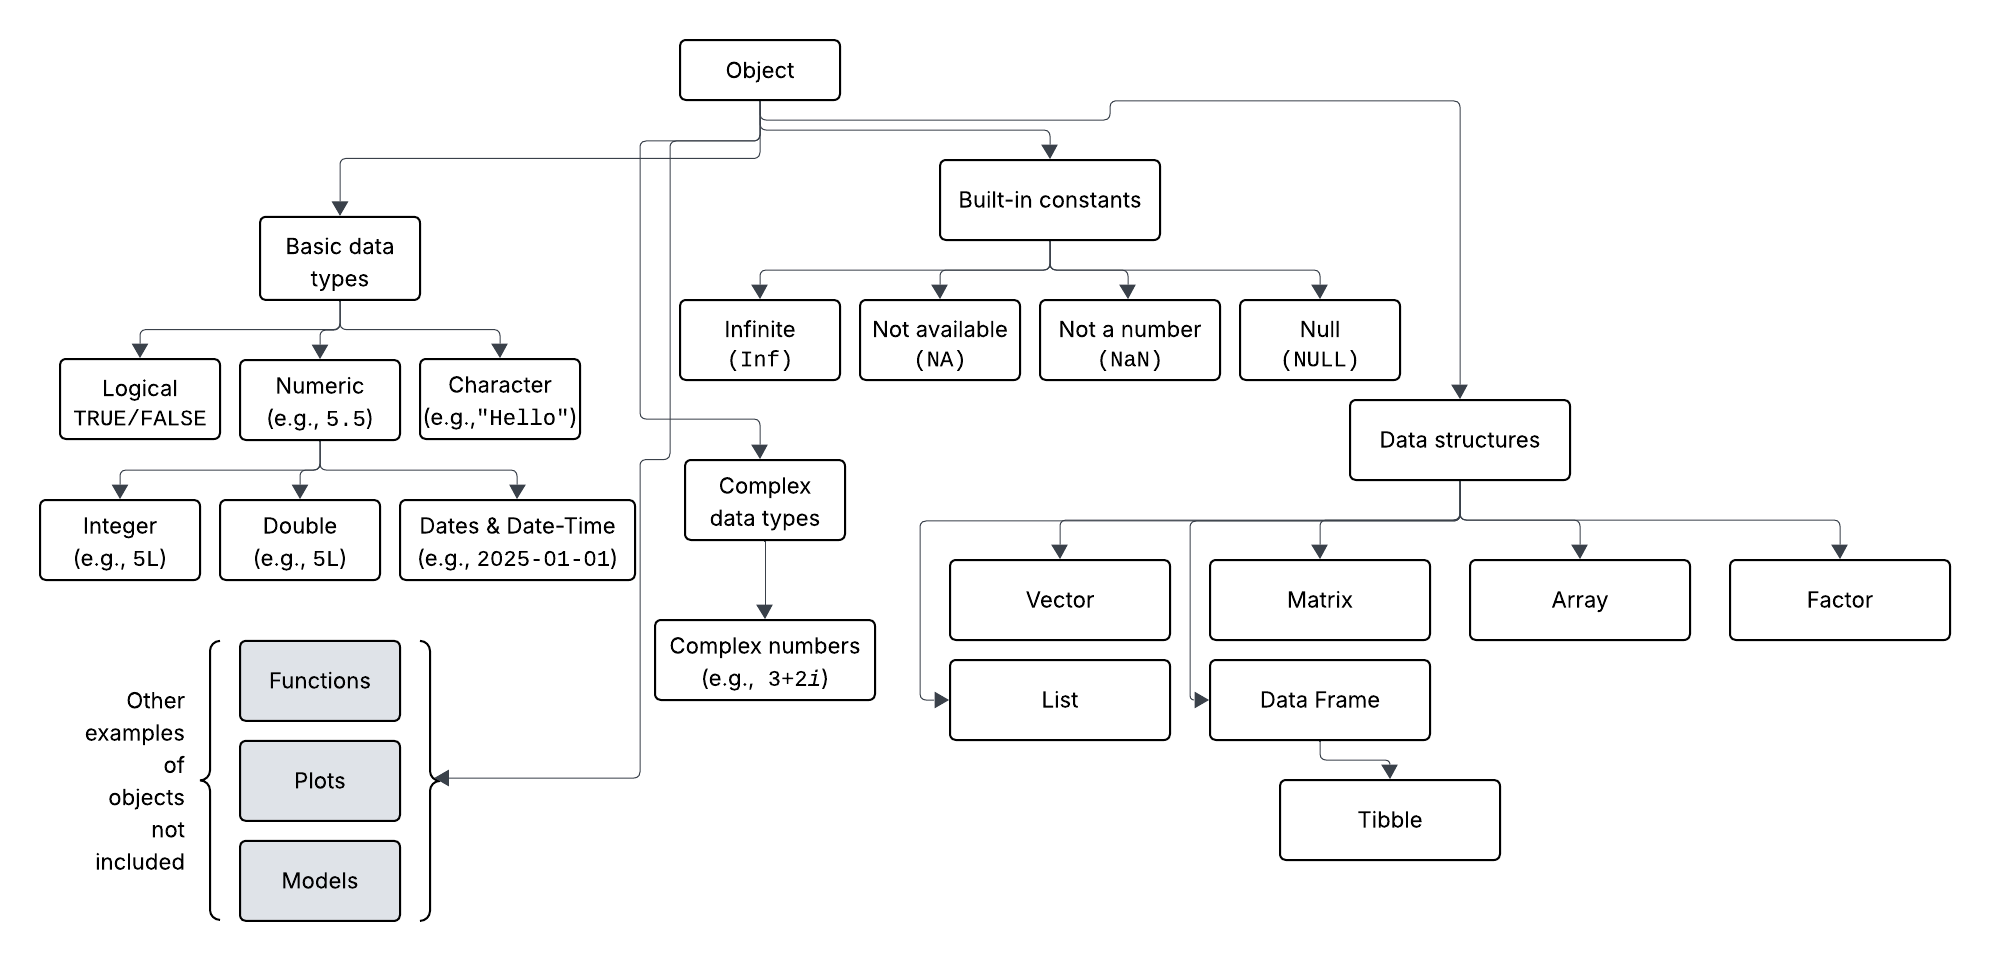
\includegraphics[width=0.95\linewidth]{images/03-ObjectDiagram} 

}

\caption{A rough diagram of the object hierarchy of what will be covered in this chapter. Most things in R descend and inherit functionality from the main Object class, and as such are related. Examples of each object type have been presented in parentheses where possible. The information in the grey boxes either has been or will be covered in other chapters, and this does not include topics such as user-defined classes and objects.}\label{fig:object-hierarchy}
\end{figure}

Figure \ref{fig:object-hierarchy} provides a rough outline of the chapter to come, starting with the basic and complex data types in Section \ref{sec:dataTypes}, followed by built-in constants in Section \ref{sec:builtInConstants}, then data structures in Section \ref{sec:dataStructure}, and concluding with data manipulation in Sections \ref{sec:tidyverse}-\ref{sec:logicFlow} and merging data sets in Section \ref{sec:merging}.

\section{Data Types}\label{sec:dataTypes}

R has object-oriented programming capabilities, which means that almost everything in R is an object which has a \textbf{class}. The class defines the object's type (e.g., what information it can hold) and how R behaves when functions (see Section \ref{sec:functions}) are applied to it. This means that regardless of object type, the \texttt{class} function can be used to check the data type.

Define a function and check its class:

\begin{Shaded}
\begin{Highlighting}[]
\CommentTok{\# Define the function}
\NormalTok{a }\OtherTok{\textless{}{-}} \ControlFlowTok{function}\NormalTok{()\{}
\NormalTok{    base}\SpecialCharTok{::}\FunctionTok{print}\NormalTok{(}\StringTok{"hello world"}\NormalTok{)}
\NormalTok{\}}

\CommentTok{\# Check the class}
\NormalTok{base}\SpecialCharTok{::}\FunctionTok{class}\NormalTok{(a)}
\end{Highlighting}
\end{Shaded}

\begin{verbatim}
## [1] "function"
\end{verbatim}

These objects can be used to store different types of data, and each data type has inherently distinct properties, allowing R to use them for various tasks. In R, variables do not need to be declared as a specific type of data, as shown in Chapter \ref{ch-2}; an object can change type after having been set. This is distinctly different from languages such as Java and C++.

\subsection{Logical (Booleans)}\label{sec:boolean}

One of the most basic and simple data types in R are \textbf{logical} or \textbf{boolean} values, which can either be \textbf{\texttt{TRUE}} (\texttt{T} also works) or \textbf{\texttt{FALSE}} (or \texttt{F}).

Check the class:

\begin{Shaded}
\begin{Highlighting}[]
\CommentTok{\# Of the straight boolean}
\NormalTok{base}\SpecialCharTok{::}\FunctionTok{class}\NormalTok{(}\ConstantTok{TRUE}\NormalTok{)}
\end{Highlighting}
\end{Shaded}

\begin{verbatim}
## [1] "logical"
\end{verbatim}

\begin{Shaded}
\begin{Highlighting}[]
\CommentTok{\# Or of an assigned variable}
\NormalTok{a }\OtherTok{\textless{}{-}} \ConstantTok{FALSE}
\NormalTok{base}\SpecialCharTok{::}\FunctionTok{class}\NormalTok{(a)}
\end{Highlighting}
\end{Shaded}

\begin{verbatim}
## [1] "logical"
\end{verbatim}

Rather self-explanatory, \textbf{logical} data are most often used when one is checking to see if an expression is either \texttt{TRUE} or \texttt{FALSE}. That is, when comparing values or objects, such as \texttt{x\ \textgreater{}\ 15} or \texttt{x\ \textless{}\ y}.

Examples of expressions and their boolean results:

\begin{Shaded}
\begin{Highlighting}[]
\CommentTok{\# Expressions comparing two numbers}
\DecValTok{1} \SpecialCharTok{\textless{}} \DecValTok{2}
\end{Highlighting}
\end{Shaded}

\begin{verbatim}
## [1] TRUE
\end{verbatim}

\begin{Shaded}
\begin{Highlighting}[]
\DecValTok{2} \SpecialCharTok{==} \DecValTok{2}
\end{Highlighting}
\end{Shaded}

\begin{verbatim}
## [1] TRUE
\end{verbatim}

\begin{Shaded}
\begin{Highlighting}[]
\DecValTok{2} \SpecialCharTok{\textgreater{}} \DecValTok{1}
\end{Highlighting}
\end{Shaded}

\begin{verbatim}
## [1] TRUE
\end{verbatim}

\begin{Shaded}
\begin{Highlighting}[]
\CommentTok{\# Or comparing two variables}
\NormalTok{a }\OtherTok{\textless{}{-}} \DecValTok{1}
\NormalTok{b }\OtherTok{\textless{}{-}} \DecValTok{2}
\NormalTok{a }\SpecialCharTok{\textless{}}\NormalTok{ b}
\end{Highlighting}
\end{Shaded}

\begin{verbatim}
## [1] TRUE
\end{verbatim}

\subsubsection{Boolean with Comparison Operators}\label{boolean-with-comparison-operators}

\textbf{Comparison operators} are used to compare two values and return a \textbf{boolean} value based on the result. The operators and examples are described in Table \ref{tab:operators}.

\begin{table}

\caption{\label{tab:operators}A table of the most common operators used to compare two values.}
\centering
\begin{tabular}[t]{l|l|l}
\hline
Operator & Description & Example\\
\hline
> & Greater than & `2 > 1` returns `TRUE`\\
\hline
< & Less than & `2 < 1` returns `FALSE`\\
\hline
== & Equals to & `2 == 2` returns `TRUE`\\
\hline
!= & Not equal to & `2 != 2` returns `FALSE`\\
\hline
>= & Greater than or equal to & `2 >= 1` returns `TRUE`\\
\hline
<= & Less than or equal to & `2 <= 1` returns `FALSE`\\
\hline
\end{tabular}
\end{table}

\subsubsection{Boolean with Logical Operators}\label{sec:logicalOperators}

Following on, \textbf{logical operators} are used to compare the output of two comparisons. The three options in R are:

\begin{enumerate}
\def\labelenumi{\arabic{enumi}.}
\tightlist
\item
  \textbf{\texttt{AND}} operator (\texttt{\&}),
\item
  \textbf{\texttt{OR}} operator (\texttt{\textbar{}}),
\item
  and \textbf{\texttt{NOT}} operator (\texttt{!})
\end{enumerate}

The \textbf{\texttt{AND}} operator takes a logical input on either side of the \texttt{\&} and returns \texttt{TRUE} only if \textbf{both} sides of the \texttt{\&} evaluate to \texttt{TRUE}.

For example:

\begin{Shaded}
\begin{Highlighting}[]
\CommentTok{\# The following will evaluate to true:}
\ConstantTok{TRUE} \SpecialCharTok{\&} \ConstantTok{TRUE} 
\end{Highlighting}
\end{Shaded}

\begin{verbatim}
## [1] TRUE
\end{verbatim}

\begin{Shaded}
\begin{Highlighting}[]
\CommentTok{\# while the following will evaluate to false}
\ConstantTok{FALSE} \SpecialCharTok{\&} \ConstantTok{TRUE}
\end{Highlighting}
\end{Shaded}

\begin{verbatim}
## [1] FALSE
\end{verbatim}

\begin{Shaded}
\begin{Highlighting}[]
\ConstantTok{TRUE} \SpecialCharTok{\&} \ConstantTok{FALSE}
\end{Highlighting}
\end{Shaded}

\begin{verbatim}
## [1] FALSE
\end{verbatim}

What do you think \texttt{FALSE\ \&\ FALSE} will evaluate to? Note that both sides of \texttt{\&} are the same.

Using the same format, the \textbf{\texttt{OR}} takes a logical input on either side of the \texttt{\textbar{}} and returns \texttt{TRUE} if \textbf{either} side of the \texttt{\textbar{}} evaluate to \texttt{TRUE}. As only one of the arguments needs to evaluate to \texttt{TRUE} for \textbf{\texttt{OR}} to be true, if the first argument evaluates as \texttt{TRUE}, the second will not be checked.

What do you expect the following to evaluate?
1. \texttt{TRUE\ \textbar{}\ TRUE}
2. \texttt{FALSE\ \textbar{}\ FALSE}
3. \texttt{TRUE\ \textbar{}\ FALSE}
4. \texttt{FALSE\ \textbar{}\ TRUE}

Conversely, the \textbf{\texttt{NOT}} operator \texttt{!} takes one logical input and negates (flips) it. So, if a value is \texttt{TRUE}, using \texttt{!} would negate it and turn it to \texttt{FALSE}, and vice versa.

For example:

\begin{Shaded}
\begin{Highlighting}[]
\CommentTok{\# The following will evaluate to true:}
\SpecialCharTok{!}\ConstantTok{FALSE} 
\end{Highlighting}
\end{Shaded}

\begin{verbatim}
## [1] TRUE
\end{verbatim}

\begin{Shaded}
\begin{Highlighting}[]
\SpecialCharTok{!}\ConstantTok{FALSE} \SpecialCharTok{\&} \ConstantTok{TRUE}
\end{Highlighting}
\end{Shaded}

\begin{verbatim}
## [1] TRUE
\end{verbatim}

\begin{Shaded}
\begin{Highlighting}[]
\CommentTok{\# while the following will evaluate to false}
\SpecialCharTok{!}\ConstantTok{TRUE}
\end{Highlighting}
\end{Shaded}

\begin{verbatim}
## [1] FALSE
\end{verbatim}

\begin{Shaded}
\begin{Highlighting}[]
\SpecialCharTok{!}\ConstantTok{TRUE} \SpecialCharTok{\&} \ConstantTok{TRUE}
\end{Highlighting}
\end{Shaded}

\begin{verbatim}
## [1] FALSE
\end{verbatim}

Finally, the \textbf{\texttt{NOT}} operator can be combined with comparisons using parentheses to build more complicated comparisons. For example, \texttt{!(x\ \textgreater{}\ 10)} is equivalent to saying that \texttt{x} is not greater than 10, which means that it is less than or equal to 10, i.e., \texttt{x\ \textless{}=\ 10}. As an aside, the \textbf{\texttt{NOT}} operator (\texttt{!}) can also be used on functions that evaluate to booleans.

\subsubsection{Operators and Precedence}\label{operators-and-precedence}

In a similar vein to the order of operations in mathematics, R executes code based on a precedence, analogous to the mathematical order of operations (remember the acronym PEMDAS or BODMAS from maths at school?). In R and computational languages more broadly, this expanded to include things such as variable assignment logic.

\begin{table}

\caption{\label{tab:precedence}A subset of the most common operators grouped and listed by order of precedence, i.e., order of execution.}
\centering
\begin{tabular}[t]{l|l|l}
\hline
Order & Operator & Meaning\\
\hline
1. & :: & Access functions and variables in a namespace\\
\hline
2. & \$ & Component extraction\\
\hline
3. & [, [[ & Indexing\\
\hline
4. & \textasciicircum{} & Exponentiation\\
\hline
5. & +, - & Characters representing the sign of a number (i.e., unary minus or plus)\\
\hline
6. & : & Sequence operator (e.g., 1:5)\\
\hline
7. & \%\%, |>, \%*\%, etc. & Special operators (e.g., \%\% for modulus, the remainder from division)\\
\hline
8. & <, >, <=, >=, ==, != & Ordering and comparison\\
\hline
9. & ! & Negation\\
\hline
10. & \& & Logical AND\\
\hline
11. & | & Logical OR\\
\hline
12. & \textasciitilde{} & As found in formulae\\
\hline
13. & -> & Rightward assignment\\
\hline
14. & <- & Assignment (right to left)\\
\hline
15. & = & Assignment (right to left)\\
\hline
16. & ? & Help\\
\hline
\end{tabular}
\end{table}

In particular, assignment operators have the (almost) lowest precedence; this means that variable assignment is the last thing that should be executed when processing a row of code. As seen in Table \ref{tab:precedence}, part of the reason for preferring a \texttt{\textless{}-} assignment operator for variables over a more traditional-looking \texttt{=}, is that R gives the former a higher precedence. Parentheses blocks, denoted with \texttt{()}, can be used to group comparisons or mathematical statements together to ensure that the code block inside is evaluated before continuing to the rest of the code.

The logical \texttt{AND} (\texttt{\&}) has higher precedence than \texttt{OR} (\texttt{\textbar{}}):

\begin{Shaded}
\begin{Highlighting}[]
\ConstantTok{TRUE} \SpecialCharTok{|} \ConstantTok{TRUE} \SpecialCharTok{\&} \ConstantTok{FALSE} \CommentTok{\# this is equivalent to the following}
\end{Highlighting}
\end{Shaded}

\begin{verbatim}
## [1] TRUE
\end{verbatim}

\begin{Shaded}
\begin{Highlighting}[]
\ConstantTok{TRUE} \SpecialCharTok{|}\NormalTok{ (}\ConstantTok{TRUE} \SpecialCharTok{\&} \ConstantTok{FALSE}\NormalTok{)}
\end{Highlighting}
\end{Shaded}

\begin{verbatim}
## [1] TRUE
\end{verbatim}

\begin{Shaded}
\begin{Highlighting}[]
\CommentTok{\# Whereas, the "()" force the OR ("|") to evaluate first:}
\NormalTok{(}\ConstantTok{TRUE} \SpecialCharTok{|} \ConstantTok{TRUE}\NormalTok{) }\SpecialCharTok{\&} \ConstantTok{FALSE} 
\end{Highlighting}
\end{Shaded}

\begin{verbatim}
## [1] FALSE
\end{verbatim}

What happens if you flip the exercise, replacing the \texttt{ORs} with \texttt{ANDs}? Is this what you expect?

\subsection{Numeric}\label{sec:numeric}

A \textbf{Numeric} object or value contains only numbers (e.g., 1, 2, 5.5, pi, etc.).

Check the class:

\begin{Shaded}
\begin{Highlighting}[]
\CommentTok{\# Of the straight number}
\NormalTok{base}\SpecialCharTok{::}\FunctionTok{class}\NormalTok{(}\FloatTok{5.5}\NormalTok{)}
\end{Highlighting}
\end{Shaded}

\begin{verbatim}
## [1] "numeric"
\end{verbatim}

\begin{Shaded}
\begin{Highlighting}[]
\CommentTok{\# Or of an assigned variable}
\NormalTok{a }\OtherTok{\textless{}{-}} \DecValTok{5}
\NormalTok{base}\SpecialCharTok{::}\FunctionTok{class}\NormalTok{(a)}
\end{Highlighting}
\end{Shaded}

\begin{verbatim}
## [1] "numeric"
\end{verbatim}

Alternatively, \texttt{is.numeric} can be used to check to see if an object is \textbf{numeric}.

What do you think the following code will evaluate to?

\texttt{x\ \textless{}-\ 5}
\texttt{base::print(base::is.numeric(x)\ \&\ (x\ \textless{}\ 5\ \textbar{}\ x\ ==\ 5))}

See Section \ref{sec:logicalOperators} for help with logical operators.

The numeric data type is R's default treatment for numbers and includes integers and doubles.

\subsubsection{Integer}\label{sec:int}

\textbf{Integers} are the whole numbers that come to mind when thinking about a numeric value, e.g., 1, 2, 3, or 4. Integers are specified by putting a capital \texttt{L} after an integer value.

Check the class:

\begin{Shaded}
\begin{Highlighting}[]
\CommentTok{\# Of a whole number}
\NormalTok{base}\SpecialCharTok{::}\FunctionTok{is.integer}\NormalTok{(}\DecValTok{1000}\NormalTok{)}
\end{Highlighting}
\end{Shaded}

\begin{verbatim}
## [1] FALSE
\end{verbatim}

\begin{Shaded}
\begin{Highlighting}[]
\CommentTok{\# Of a specified integer}
\NormalTok{base}\SpecialCharTok{::}\FunctionTok{class}\NormalTok{(}\DecValTok{1000}\DataTypeTok{L}\NormalTok{)}
\end{Highlighting}
\end{Shaded}

\begin{verbatim}
## [1] "integer"
\end{verbatim}

\begin{Shaded}
\begin{Highlighting}[]
\CommentTok{\# Or of an assigned variable}
\NormalTok{a }\OtherTok{\textless{}{-}} \DecValTok{5333}\DataTypeTok{L}
\NormalTok{base}\SpecialCharTok{::}\FunctionTok{class}\NormalTok{(a)}
\end{Highlighting}
\end{Shaded}

\begin{verbatim}
## [1] "integer"
\end{verbatim}

That being said, R handles the differences between the usual, unspecified numerics (see Section \ref{sec:numeric}) and integers in the background, so they are often not noticed. The value of 1,000 has been deliberately chosen to show the differences and similarities between numeric and integer values.

Background differences:

\begin{Shaded}
\begin{Highlighting}[]
\NormalTok{base}\SpecialCharTok{::}\FunctionTok{is.numeric}\NormalTok{(}\DecValTok{1000}\NormalTok{)}
\end{Highlighting}
\end{Shaded}

\begin{verbatim}
## [1] TRUE
\end{verbatim}

\begin{Shaded}
\begin{Highlighting}[]
\NormalTok{base}\SpecialCharTok{::}\FunctionTok{is.integer}\NormalTok{(}\DecValTok{1000}\NormalTok{)}
\end{Highlighting}
\end{Shaded}

\begin{verbatim}
## [1] FALSE
\end{verbatim}

\begin{Shaded}
\begin{Highlighting}[]
\NormalTok{base}\SpecialCharTok{::}\FunctionTok{is.numeric}\NormalTok{(}\DecValTok{1000}\DataTypeTok{L}\NormalTok{)}
\end{Highlighting}
\end{Shaded}

\begin{verbatim}
## [1] TRUE
\end{verbatim}

\begin{Shaded}
\begin{Highlighting}[]
\NormalTok{base}\SpecialCharTok{::}\FunctionTok{is.integer}\NormalTok{(}\DecValTok{1000}\DataTypeTok{L}\NormalTok{)}
\end{Highlighting}
\end{Shaded}

\begin{verbatim}
## [1] TRUE
\end{verbatim}

Think of \textbf{\texttt{integers}} as a subset of \textbf{\texttt{numeric}}, and follow a pattern of all \textbf{\texttt{integers}} are \textbf{\texttt{numeric}}, but not all \textbf{\texttt{numeric}} are \textbf{\texttt{integers}}.

\subsubsection{Double}\label{sec:double}

\textbf{Doubles} are any numbers that have a decimal point. Take 5.0 or 5.5 for example.

Check the class:

\begin{Shaded}
\begin{Highlighting}[]
\CommentTok{\# Of a double number}
\NormalTok{base}\SpecialCharTok{::}\FunctionTok{is.double}\NormalTok{(}\FloatTok{5.5}\NormalTok{)}
\end{Highlighting}
\end{Shaded}

\begin{verbatim}
## [1] TRUE
\end{verbatim}

\begin{Shaded}
\begin{Highlighting}[]
\NormalTok{base}\SpecialCharTok{::}\FunctionTok{typeof}\NormalTok{(}\FloatTok{5.5}\NormalTok{)}
\end{Highlighting}
\end{Shaded}

\begin{verbatim}
## [1] "double"
\end{verbatim}

As seen in Section \ref{sec:numeric}, the number 5.5 is also a \textbf{\texttt{numeric}}. Following the phrasing of integers above, all \textbf{\texttt{doubles}} are \textbf{\texttt{numeric}}, but not all \textbf{\texttt{numeric}} values are \textbf{\texttt{doubles}}.

\subsubsection{Integers Versus Doubles}\label{integers-versus-doubles}

Programmers and analysts will typically use \textbf{\texttt{integers}} when they know that decimals will never be needed, for example, when dealing with IDs. The advantage is that \textbf{\texttt{integers}} take up less memory, but the trade-off is that they can only go a little more than two billion.

Size and memory differences:

\begin{Shaded}
\begin{Highlighting}[]
\CommentTok{\# Maximum size of an integer}
\NormalTok{.Machine}\SpecialCharTok{$}\NormalTok{integer.max}
\end{Highlighting}
\end{Shaded}

\begin{verbatim}
## [1] 2147483647
\end{verbatim}

\begin{Shaded}
\begin{Highlighting}[]
\CommentTok{\# Maximum size of a double (numeric) }
\NormalTok{.Machine}\SpecialCharTok{$}\NormalTok{double.xmax}
\end{Highlighting}
\end{Shaded}

\begin{verbatim}
## [1] 1.797693e+308
\end{verbatim}

\begin{Shaded}
\begin{Highlighting}[]
\CommentTok{\# Implications of using integers versus numeric/doubles at scale (1 million)}
\NormalTok{ints }\OtherTok{\textless{}{-}}\NormalTok{ base}\SpecialCharTok{::}\FunctionTok{rep}\NormalTok{(}\DecValTok{1}\DataTypeTok{L}\NormalTok{, }\FloatTok{1e6}\NormalTok{)}
\NormalTok{numeric }\OtherTok{\textless{}{-}}\NormalTok{ base}\SpecialCharTok{::}\FunctionTok{rep}\NormalTok{(}\DecValTok{1}\NormalTok{, }\FloatTok{1e6}\NormalTok{)}

\DocumentationTok{\#\# Check memory usage }
\NormalTok{utils}\SpecialCharTok{::}\FunctionTok{object.size}\NormalTok{(ints)}
\end{Highlighting}
\end{Shaded}

\begin{verbatim}
## 4000048 bytes
\end{verbatim}

\begin{Shaded}
\begin{Highlighting}[]
\NormalTok{utils}\SpecialCharTok{::}\FunctionTok{object.size}\NormalTok{(numeric)}
\end{Highlighting}
\end{Shaded}

\begin{verbatim}
## 8000048 bytes
\end{verbatim}

This clearly shows the two-time size difference between \textbf{\texttt{integers}} and \textbf{\texttt{doubles}}, which is why it is helpful to think about data types when working with data. The absolute difference (8 MB vs.~4 MB) may look small in this toy example. However, in real world data where you have multi-million rows, it would become important, especially because R needs to store all active data in the computer memory (RAM).

One place where it pays to be aware of \textbf{\texttt{integers}} versus \textbf{\texttt{doubles}} is when dividing. The result of the division (\texttt{/}) will always be a \textbf{\texttt{double}} because it is calculated using floating-point division.

Differences in dividing:

\begin{Shaded}
\begin{Highlighting}[]
\CommentTok{\# Dividing numeric values }
\NormalTok{x }\OtherTok{\textless{}{-}} \DecValTok{5}\SpecialCharTok{/}\DecValTok{2}
\NormalTok{base}\SpecialCharTok{::}\FunctionTok{print}\NormalTok{(x)}
\end{Highlighting}
\end{Shaded}

\begin{verbatim}
## [1] 2.5
\end{verbatim}

\begin{Shaded}
\begin{Highlighting}[]
\NormalTok{base}\SpecialCharTok{::}\FunctionTok{typeof}\NormalTok{(x)}
\end{Highlighting}
\end{Shaded}

\begin{verbatim}
## [1] "double"
\end{verbatim}

\begin{Shaded}
\begin{Highlighting}[]
\CommentTok{\# Dividing integers }
\NormalTok{y }\OtherTok{\textless{}{-}} \DecValTok{4}\DataTypeTok{L}\SpecialCharTok{/}\DecValTok{2}\DataTypeTok{L}
\NormalTok{base}\SpecialCharTok{::}\FunctionTok{print}\NormalTok{(y)}
\end{Highlighting}
\end{Shaded}

\begin{verbatim}
## [1] 2
\end{verbatim}

\begin{Shaded}
\begin{Highlighting}[]
\NormalTok{base}\SpecialCharTok{::}\FunctionTok{typeof}\NormalTok{(y)}
\end{Highlighting}
\end{Shaded}

\begin{verbatim}
## [1] "double"
\end{verbatim}

Can you think of three examples of when you would want to use an integer instead of a numeric value and vice versa?

\subsubsection{Dates and Date-times}\label{sec:datesAndTimes}

\textbf{Dates} (e.g., \texttt{"2025-01-01"}) and \textbf{date-times} (e.g., \texttt{"2025-01-01\ 10:30:00"}) are grouped under numeric data types because R actually stores dates in numerical format, technically based on the difference/distance from R's origin date of 1st January 1970.

Working with time seems like an easy thing. For instance, it is easy to say that there are 365 days in a year, except for a leap year, which has 366 days. The convention, then, when converting days into years, is to split the leap day into 0.25 days per year, resulting in 365.25 days per year. Of course, time has an analogous issue surrounding daylight saving time, so one day a year will have 23 hours while another will have 25 hours. Furthermore, the application of daylight saving time is subject to various geopolitical factors. For this reason, the \texttt{lubridate} package has become the default when working with dates and times in R, and is fortunately part of the core \texttt{tidyverse} universe.

Using the diabeticLabs dataset, explore the SampleDate column

\begin{Shaded}
\begin{Highlighting}[]
\NormalTok{lab\_data }\OtherTok{\textless{}{-}}\NormalTok{ utils}\SpecialCharTok{::}\FunctionTok{read.csv}\NormalTok{(}\StringTok{"data/03{-}diabetic\_labs\_final\_with\_missing.csv"}\NormalTok{, }\AttributeTok{head =} \ConstantTok{TRUE}\NormalTok{)}

\CommentTok{\# Get a summary of the SampleDate }
\FunctionTok{head}\NormalTok{(lab\_data, }\DecValTok{3}\DataTypeTok{L}\NormalTok{)}
\end{Highlighting}
\end{Shaded}

\begin{verbatim}
##   id SampleDate SampleTime Chol   TG      HDL      LDL   Cr  BUN
## 1  5 26/01/2009   16:26:00 4.90 2.10 1.100000 2.500000 56.0 5.10
## 2  5 19/10/2012   10:22:00 3.60 5.10 0.900000 2.500000 63.0 5.00
## 3  5 19/10/2012   09:31:00 4.85 1.63 4.860753 4.860753 96.7 5.24
\end{verbatim}

\begin{Shaded}
\begin{Highlighting}[]
\CommentTok{\# Get a summary of the data}
\FunctionTok{summary}\NormalTok{(lab\_data}\SpecialCharTok{$}\NormalTok{SampleDate)}
\end{Highlighting}
\end{Shaded}

\begin{verbatim}
##    Length     Class      Mode 
##       478 character character
\end{verbatim}

\begin{Shaded}
\begin{Highlighting}[]
\CommentTok{\# check the format of the data}
\NormalTok{base}\SpecialCharTok{::}\FunctionTok{class}\NormalTok{(lab\_data}\SpecialCharTok{$}\NormalTok{SampleDate)}
\end{Highlighting}
\end{Shaded}

\begin{verbatim}
## [1] "character"
\end{verbatim}

From the \texttt{utils::head(lab\_data,\ 3L)} call, the \texttt{SampleDate} column looks like valid dates, all be it specified in a \texttt{day-month-year} format, yet the \texttt{class} indicates that the column contains characters (see Section \ref{sec:character}). If the data was used without converting it, R would not behave as expected.

Try a character string comparison

\begin{Shaded}
\begin{Highlighting}[]
\CommentTok{\# Pick out the first row of the file for simplicity}
\NormalTok{lab\_data }\OtherTok{\textless{}{-}}\NormalTok{ utils}\SpecialCharTok{::}\FunctionTok{read.csv}\NormalTok{(}\StringTok{"data/03{-}diabetic\_labs\_final\_with\_missing.csv"}\NormalTok{)}
\NormalTok{base}\SpecialCharTok{::}\FunctionTok{print}\NormalTok{(row }\OtherTok{\textless{}{-}}\NormalTok{ lab\_data[}\DecValTok{1}\NormalTok{,])}
\end{Highlighting}
\end{Shaded}

\begin{verbatim}
##   id SampleDate SampleTime Chol  TG HDL LDL Cr BUN
## 1  5 26/01/2009   16:26:00  4.9 2.1 1.1 2.5 56 5.1
\end{verbatim}

\begin{Shaded}
\begin{Highlighting}[]
\NormalTok{base}\SpecialCharTok{::}\FunctionTok{print}\NormalTok{(row}\SpecialCharTok{$}\NormalTok{SampleDate }\SpecialCharTok{\textless{}} \StringTok{"26/01/2009a"}\NormalTok{)}
\end{Highlighting}
\end{Shaded}

\begin{verbatim}
## [1] TRUE
\end{verbatim}

This evaluates to \textbf{\texttt{TRUE}} as R is lexicographically comparing two character strings rather than two dates, and the \texttt{a} at the end of \texttt{26/01/2009a} makes it longer and therefore a larger string than \texttt{26/01/2009}.

Convert to Dates:

\begin{Shaded}
\begin{Highlighting}[]
\NormalTok{lab\_data }\OtherTok{\textless{}{-}}\NormalTok{ utils}\SpecialCharTok{::}\FunctionTok{read.csv}\NormalTok{(}\StringTok{"data/03{-}diabetic\_labs\_final\_with\_missing.csv"}\NormalTok{, }\AttributeTok{head =} \ConstantTok{TRUE}\NormalTok{)}
\NormalTok{lab\_data}\SpecialCharTok{$}\NormalTok{SampleDate }\OtherTok{\textless{}{-}}\NormalTok{ base}\SpecialCharTok{::}\FunctionTok{as.Date}\NormalTok{(lab\_data}\SpecialCharTok{$}\NormalTok{SampleDate)}

\NormalTok{utils}\SpecialCharTok{::}\FunctionTok{head}\NormalTok{(lab\_data, }\AttributeTok{n =} \DecValTok{3}\DataTypeTok{L}\NormalTok{)}
\end{Highlighting}
\end{Shaded}

\begin{verbatim}
##   id SampleDate SampleTime Chol   TG      HDL      LDL   Cr  BUN
## 1  5 0026-01-20   16:26:00 4.90 2.10 1.100000 2.500000 56.0 5.10
## 2  5 0019-10-20   10:22:00 3.60 5.10 0.900000 2.500000 63.0 5.00
## 3  5 0019-10-20   09:31:00 4.85 1.63 4.860753 4.860753 96.7 5.24
\end{verbatim}

So, this kind of worked, but the date format isn't quite as expected; the year is slightly off. To prevent this from happening, specify the format of the date, where \texttt{\%d}, specifies the location of the days, \texttt{\%m} specifies the location of the month, and \texttt{\%Y} specifies the location of the year, all stitched together with the linking character \texttt{/} in this case.

Convert to Dates using base and lubridate's as\_date:

\begin{Shaded}
\begin{Highlighting}[]
\NormalTok{lab\_data }\OtherTok{\textless{}{-}}\NormalTok{ utils}\SpecialCharTok{::}\FunctionTok{read.csv}\NormalTok{(}\StringTok{"data/03{-}diabetic\_labs\_final\_with\_missing.csv"}\NormalTok{)}

\CommentTok{\# Using base R}
\NormalTok{lab\_data}\SpecialCharTok{$}\NormalTok{SampleDate }\OtherTok{\textless{}{-}}\NormalTok{ base}\SpecialCharTok{::}\FunctionTok{as.Date}\NormalTok{(lab\_data}\SpecialCharTok{$}\NormalTok{SampleDate, }\AttributeTok{format =} \StringTok{"\%d/\%m/\%Y"}\NormalTok{)}
\NormalTok{utils}\SpecialCharTok{::}\FunctionTok{head}\NormalTok{(lab\_data, }\AttributeTok{n =} \DecValTok{3}\DataTypeTok{L}\NormalTok{)}
\end{Highlighting}
\end{Shaded}

\begin{verbatim}
##   id SampleDate SampleTime Chol   TG      HDL      LDL   Cr  BUN
## 1  5 2009-01-26   16:26:00 4.90 2.10 1.100000 2.500000 56.0 5.10
## 2  5 2012-10-19   10:22:00 3.60 5.10 0.900000 2.500000 63.0 5.00
## 3  5 2012-10-19   09:31:00 4.85 1.63 4.860753 4.860753 96.7 5.24
\end{verbatim}

\begin{Shaded}
\begin{Highlighting}[]
\CommentTok{\# Using lubridate}
\NormalTok{lab\_data }\OtherTok{\textless{}{-}}\NormalTok{ utils}\SpecialCharTok{::}\FunctionTok{read.csv}\NormalTok{(}\StringTok{"data/03{-}diabetic\_labs\_final\_with\_missing.csv"}\NormalTok{)}
\NormalTok{lab\_data}\SpecialCharTok{$}\NormalTok{SampleDate }\OtherTok{\textless{}{-}}\NormalTok{ lubridate}\SpecialCharTok{::}\FunctionTok{as\_date}\NormalTok{(}
\NormalTok{  lab\_data}\SpecialCharTok{$}\NormalTok{SampleDate, }\AttributeTok{format =} \StringTok{"\%d/\%m/\%Y"}\NormalTok{)}
  
\NormalTok{utils}\SpecialCharTok{::}\FunctionTok{head}\NormalTok{(lab\_data, }\AttributeTok{n =} \DecValTok{3}\DataTypeTok{L}\NormalTok{)}
\end{Highlighting}
\end{Shaded}

\begin{verbatim}
##   id SampleDate SampleTime Chol   TG      HDL      LDL   Cr  BUN
## 1  5 2009-01-26   16:26:00 4.90 2.10 1.100000 2.500000 56.0 5.10
## 2  5 2012-10-19   10:22:00 3.60 5.10 0.900000 2.500000 63.0 5.00
## 3  5 2012-10-19   09:31:00 4.85 1.63 4.860753 4.860753 96.7 5.24
\end{verbatim}

Now that formatting is correct, let's convert to Dates and try again:

\begin{Shaded}
\begin{Highlighting}[]
\NormalTok{lab\_data }\OtherTok{\textless{}{-}}\NormalTok{ utils}\SpecialCharTok{::}\FunctionTok{read.csv}\NormalTok{(}\StringTok{"data/03{-}diabetic\_labs\_final\_with\_missing.csv"}\NormalTok{, }\AttributeTok{head =} \ConstantTok{TRUE}\NormalTok{)}
\NormalTok{lab\_data}\SpecialCharTok{$}\NormalTok{SampleDate }\OtherTok{\textless{}{-}}\NormalTok{ lubridate}\SpecialCharTok{::}\FunctionTok{as\_date}\NormalTok{(lab\_data}\SpecialCharTok{$}\NormalTok{SampleDate, }\AttributeTok{format =} \StringTok{"\%d/\%m/\%Y"}\NormalTok{)}

\CommentTok{\# Pick out the 1st row of the file for simplicity}
\NormalTok{base}\SpecialCharTok{::}\FunctionTok{print}\NormalTok{(row }\OtherTok{\textless{}{-}}\NormalTok{ lab\_data[}\DecValTok{1}\NormalTok{,])}
\end{Highlighting}
\end{Shaded}

\begin{verbatim}
##   id SampleDate SampleTime Chol  TG HDL LDL Cr BUN
## 1  5 2009-01-26   16:26:00  4.9 2.1 1.1 2.5 56 5.1
\end{verbatim}

\begin{Shaded}
\begin{Highlighting}[]
\CommentTok{\# check the comparison of Date and String }
\NormalTok{base}\SpecialCharTok{::}\FunctionTok{print}\NormalTok{(row}\SpecialCharTok{$}\NormalTok{SampleDate }\SpecialCharTok{\textless{}} \StringTok{"2009{-}01{-}26a"}\NormalTok{)}
\end{Highlighting}
\end{Shaded}

\begin{verbatim}
## [1] FALSE
\end{verbatim}

\begin{Shaded}
\begin{Highlighting}[]
\CommentTok{\# check the comparison of Date and character string that can be coerced to date }
\NormalTok{base}\SpecialCharTok{::}\FunctionTok{print}\NormalTok{(row}\SpecialCharTok{$}\NormalTok{SampleDate }\SpecialCharTok{\textless{}=} \StringTok{"2009{-}01{-}26"}\NormalTok{)}
\end{Highlighting}
\end{Shaded}

\begin{verbatim}
## [1] TRUE
\end{verbatim}

\begin{Shaded}
\begin{Highlighting}[]
\CommentTok{\# check the comparison of Date and Date }
\NormalTok{base}\SpecialCharTok{::}\FunctionTok{print}\NormalTok{(row}\SpecialCharTok{$}\NormalTok{SampleDate }\SpecialCharTok{\textless{}=}\NormalTok{ lubridate}\SpecialCharTok{::}\FunctionTok{as\_date}\NormalTok{(}\StringTok{"2009{-}01{-}27"}\NormalTok{))}
\end{Highlighting}
\end{Shaded}

\begin{verbatim}
## [1] TRUE
\end{verbatim}

In the first comparison of dates and characters, R is trying to coerce the character string to a date. This fails and therefore returns \textbf{\texttt{FALSE}}. In the second such example, without the \texttt{a}, R can coerce the character string to a date and perform the comparison, where the dates are evaluated to be equal. The third example is preferable because it explicitly says that \texttt{2009-01-27} is a date.

Try summary and class one more time:

\begin{Shaded}
\begin{Highlighting}[]
\NormalTok{lab\_data }\OtherTok{\textless{}{-}}\NormalTok{ utils}\SpecialCharTok{::}\FunctionTok{read.csv}\NormalTok{(}\StringTok{"data/03{-}diabetic\_labs\_final\_with\_missing.csv"}\NormalTok{, }\AttributeTok{head =} \ConstantTok{TRUE}\NormalTok{)}
\NormalTok{lab\_data}\SpecialCharTok{$}\NormalTok{SampleDate }\OtherTok{\textless{}{-}} \FunctionTok{as.Date}\NormalTok{(lab\_data}\SpecialCharTok{$}\NormalTok{SampleDate, }\AttributeTok{format =} \StringTok{"\%d/\%m/\%Y"}\NormalTok{)}

\NormalTok{base}\SpecialCharTok{::}\FunctionTok{summary}\NormalTok{(lab\_data}\SpecialCharTok{$}\NormalTok{SampleDate)}
\end{Highlighting}
\end{Shaded}

\begin{verbatim}
##         Min.      1st Qu.       Median         Mean      3rd Qu.         Max. 
## "2009-01-01" "2010-01-01" "2011-02-27" "2011-01-21" "2012-01-22" "2012-12-31"
\end{verbatim}

\begin{Shaded}
\begin{Highlighting}[]
\NormalTok{base}\SpecialCharTok{::}\FunctionTok{class}\NormalTok{(lab\_data}\SpecialCharTok{$}\NormalTok{SampleDate)}
\end{Highlighting}
\end{Shaded}

\begin{verbatim}
## [1] "Date"
\end{verbatim}

From this it follows that \texttt{SampleDate} is from the date class and the minimum (\texttt{Min.}) date is the 1st of January 2009. For continuous data, the \texttt{summary} function also provides the first quartile (\texttt{1st\ Qu.}), median (\texttt{Median}), mean (\texttt{Mean}), third quartile (\texttt{3rd\ Qu.}), and maximum (\texttt{Max.}) values. As has been alluded to throughout the section, dates can and are stored in different formats, and R might not recognise the date as a \texttt{Date} object during import. The alternative to specifying the \texttt{format\ =} in \texttt{as\_date}, there are a couple of functions from the \texttt{lubridate} package that respecify the format:

Creating \texttt{Date} objects from character strings using lubridate and checking the class:

\begin{Shaded}
\begin{Highlighting}[]
\FunctionTok{library}\NormalTok{(lubridate)}
\NormalTok{lubridate}\SpecialCharTok{::}\FunctionTok{is.Date}\NormalTok{(lubridate}\SpecialCharTok{::}\FunctionTok{dmy}\NormalTok{(}\StringTok{\textquotesingle{}18{-}09{-}2025\textquotesingle{}}\NormalTok{))}
\end{Highlighting}
\end{Shaded}

\begin{verbatim}
## [1] TRUE
\end{verbatim}

\begin{Shaded}
\begin{Highlighting}[]
\NormalTok{lubridate}\SpecialCharTok{::}\FunctionTok{is.Date}\NormalTok{(lubridate}\SpecialCharTok{::}\FunctionTok{mdy}\NormalTok{(}\StringTok{\textquotesingle{}09{-}18{-}2025\textquotesingle{}}\NormalTok{))}
\end{Highlighting}
\end{Shaded}

\begin{verbatim}
## [1] TRUE
\end{verbatim}

\begin{Shaded}
\begin{Highlighting}[]
\NormalTok{lubridate}\SpecialCharTok{::}\FunctionTok{is.Date}\NormalTok{(lubridate}\SpecialCharTok{::}\FunctionTok{ymd}\NormalTok{(}\StringTok{\textquotesingle{}2025{-}09{-}18\textquotesingle{}}\NormalTok{))}
\end{Highlighting}
\end{Shaded}

\begin{verbatim}
## [1] TRUE
\end{verbatim}

Finally, \textbf{date-time} objects add a time component to the date (e.g., \texttt{lubridate::as\_date(\textquotesingle{}2025-09-19\textquotesingle{})} is the year-month-day Date format, while \texttt{lubridate::as\_datetime(\textquotesingle{}2025-09-19\ 14:30:00\textquotesingle{})} adds the 24-hour time down to the second).

Use as\_datetime to convert SampleTime to date-time

\begin{Shaded}
\begin{Highlighting}[]
\NormalTok{lab\_data }\OtherTok{\textless{}{-}}\NormalTok{ utils}\SpecialCharTok{::}\FunctionTok{read.csv}\NormalTok{(}\StringTok{"data/03{-}diabetic\_labs\_final\_with\_missing.csv"}\NormalTok{)}

\NormalTok{lab\_data}\SpecialCharTok{$}\NormalTok{SampleTime }\OtherTok{\textless{}{-}}\NormalTok{ lubridate}\SpecialCharTok{::}\FunctionTok{as\_datetime}\NormalTok{(}
\NormalTok{  lab\_data}\SpecialCharTok{$}\NormalTok{SampleTime, }\AttributeTok{format =} \StringTok{"\%H:\%M:\%S"}\NormalTok{)}
  
\NormalTok{utils}\SpecialCharTok{::}\FunctionTok{head}\NormalTok{(lab\_data, }\AttributeTok{n =} \DecValTok{3}\DataTypeTok{L}\NormalTok{)}
\end{Highlighting}
\end{Shaded}

\begin{verbatim}
##   id SampleDate          SampleTime Chol   TG      HDL      LDL   Cr  BUN
## 1  5 26/01/2009 0000-01-01 16:26:00 4.90 2.10 1.100000 2.500000 56.0 5.10
## 2  5 19/10/2012 0000-01-01 10:22:00 3.60 5.10 0.900000 2.500000 63.0 5.00
## 3  5 19/10/2012 0000-01-01 09:31:00 4.85 1.63 4.860753 4.860753 96.7 5.24
\end{verbatim}

Note that the date part of the date-time is a nonsensical \texttt{0000-01-01}. The \texttt{as\_hms} function within the \texttt{hms} package allows for the date component to be removed.

Use as\_datetime and as\_hms to store just the time component of date-time

\begin{Shaded}
\begin{Highlighting}[]
\NormalTok{lab\_data }\OtherTok{\textless{}{-}}\NormalTok{ utils}\SpecialCharTok{::}\FunctionTok{read.csv}\NormalTok{(}\StringTok{"data/03{-}diabetic\_labs\_final\_with\_missing.csv"}\NormalTok{)}

\NormalTok{lab\_data}\SpecialCharTok{$}\NormalTok{SampleTime }\OtherTok{\textless{}{-}}\NormalTok{ hms}\SpecialCharTok{::}\FunctionTok{as\_hms}\NormalTok{(lubridate}\SpecialCharTok{::}\FunctionTok{as\_datetime}\NormalTok{(}
\NormalTok{  lab\_data}\SpecialCharTok{$}\NormalTok{SampleTime, }\AttributeTok{format =} \StringTok{"\%H:\%M:\%S"}\NormalTok{))}
  
\NormalTok{utils}\SpecialCharTok{::}\FunctionTok{head}\NormalTok{(lab\_data, }\AttributeTok{n =} \DecValTok{3}\DataTypeTok{L}\NormalTok{)}
\end{Highlighting}
\end{Shaded}

\begin{verbatim}
##   id SampleDate SampleTime Chol   TG      HDL      LDL   Cr  BUN
## 1  5 26/01/2009   16:26:00 4.90 2.10 1.100000 2.500000 56.0 5.10
## 2  5 19/10/2012   10:22:00 3.60 5.10 0.900000 2.500000 63.0 5.00
## 3  5 19/10/2012   09:31:00 4.85 1.63 4.860753 4.860753 96.7 5.24
\end{verbatim}

This is the jumping-off point for data cleaning.

\subsection{Character}\label{sec:character}

Roughly speaking, a \textbf{character} is anything that can be typed on a keyboard, as long as it is encapsulated in a pair of quotes (\texttt{""}). A \textbf{character string} is a series of characters within a pair of quotes.

Check the class:

\begin{Shaded}
\begin{Highlighting}[]
\CommentTok{\# Of the straight character}
\NormalTok{base}\SpecialCharTok{::}\FunctionTok{class}\NormalTok{(}\StringTok{"BMI"}\NormalTok{)}
\end{Highlighting}
\end{Shaded}

\begin{verbatim}
## [1] "character"
\end{verbatim}

\begin{Shaded}
\begin{Highlighting}[]
\CommentTok{\# Or of an assigned variable (note the quotes)}
\NormalTok{a }\OtherTok{\textless{}{-}} \StringTok{"body mass index"}
\FunctionTok{class}\NormalTok{(a)}
\end{Highlighting}
\end{Shaded}

\begin{verbatim}
## [1] "character"
\end{verbatim}

For example, ``\textbf{\hyperref[acronyms_BMI]{body mass index (BMI)}}'' and ``body mass index'' are each character objects with a single character value (the string). Notably, R allows single and double quotes to be used to encapsulate and denote character strings; however, they must be used in pairs (i.e., whatever symbol starts the character string must \textbf{also} end the character string). Analogously to checking the class of numeric objects, \texttt{is.character} can be used to check whether an object is a character string.

What do you expect the class of \texttt{"TRUE"} to be? Try and see. Is this what you expected?

\subsection{Complex}\label{sec:complex}

\textbf{Complex} values are included here for completeness, but something probably went wrong if they appear in the day-to-day health data science work. Briefly, \textbf{complex} values are expressed in the form a + bi, where a and b are the ``real'' numbers (i.e., numeric), and i is the imaginary unit, derived from the square root of -1.

Check the class:

\begin{Shaded}
\begin{Highlighting}[]
\CommentTok{\# Of the straight complex number}
\FunctionTok{class}\NormalTok{(}\DecValTok{2}\DataTypeTok{i}\NormalTok{)}
\end{Highlighting}
\end{Shaded}

\begin{verbatim}
## [1] "complex"
\end{verbatim}

\begin{Shaded}
\begin{Highlighting}[]
\FunctionTok{is.complex}\NormalTok{(}\DecValTok{2}\DataTypeTok{i}\NormalTok{)}
\end{Highlighting}
\end{Shaded}

\begin{verbatim}
## [1] TRUE
\end{verbatim}

\begin{Shaded}
\begin{Highlighting}[]
\CommentTok{\# Or of an assigned variable}
\NormalTok{a }\OtherTok{\textless{}{-}} \DecValTok{3}\SpecialCharTok{+} \DecValTok{2}\DataTypeTok{i}
\FunctionTok{class}\NormalTok{(a)}
\end{Highlighting}
\end{Shaded}

\begin{verbatim}
## [1] "complex"
\end{verbatim}

Unless explicitly working with \textbf{complex} numbers, start debugging and looking for where negative numbers could be produced when \texttt{class} returns ``complex''.

\section{Important Built-in Constants}\label{sec:builtInConstants}

This section builds on the concept of reserved words presented in Section \ref{sec:reservedWords}. The built-in \textbf{constants} is a type of reserved word and represents common fixed values or special cases of data. They are built into R, and as such, are always there and do not need to be created.

\subsection{Infinite}\label{sec:infinite}

\textbf{Infinite} values in R are stored as either \textbf{\texttt{-Inf}} for negative infinity, and \textbf{\texttt{Inf}} for positive infinity values. These are useful in mathematical computations that result in values that are beyond the largest representable number.

An example of \texttt{Inf}, where a value is divided by zero:

\begin{Shaded}
\begin{Highlighting}[]
\NormalTok{i }\OtherTok{\textless{}{-}} \DecValTok{5}\SpecialCharTok{/}\DecValTok{0}
\FunctionTok{print}\NormalTok{(i)}
\end{Highlighting}
\end{Shaded}

\begin{verbatim}
## [1] Inf
\end{verbatim}

\subsection{Missing Data}\label{sec:missingData}

The next couple of sections will use the \texttt{diabetic} dataset that's part of the \texttt{survival} package, combined with blood test data modified from the Health Test by Blood Dataset.

\subsubsection{\texorpdfstring{Not available (\texttt{NA})}{Not available (NA)}}\label{sec:na}

\textbf{\texttt{\textbackslash{}acr\{NA\}}}, meaning not available, is generally used and interpreted as a missing value. It is important to note that R often, but not always, defaults to allowing \texttt{**\textbackslash{}acr\{NA\}**} values to cause problems so that missing values are not missed by default. The Health Test by Blood Dataset has been deliberately modified to introduce \textbf{\texttt{\textbackslash{}acr\{NA\}}} values to help illustrate how to handle them.

An example of how data are handled differently depending on \texttt{rm.na} is provided:

\begin{Shaded}
\begin{Highlighting}[]
\NormalTok{lab\_data }\OtherTok{\textless{}{-}}\NormalTok{ utils}\SpecialCharTok{::}\FunctionTok{read.csv}\NormalTok{(}\StringTok{"data/03{-}diabetic\_labs\_final\_with\_missing.csv"}\NormalTok{, }\AttributeTok{head =} \ConstantTok{TRUE}\NormalTok{)}

\CommentTok{\# Check out the top of the file}
\NormalTok{utils}\SpecialCharTok{::}\FunctionTok{head}\NormalTok{(lab\_data)}
\end{Highlighting}
\end{Shaded}

\begin{verbatim}
##   id SampleDate SampleTime Chol   TG      HDL      LDL   Cr  BUN
## 1  5 26/01/2009   16:26:00 4.90 2.10 1.100000 2.500000 56.0 5.10
## 2  5 19/10/2012   10:22:00 3.60 5.10 0.900000 2.500000 63.0 5.00
## 3  5 19/10/2012   09:31:00 4.85 1.63 4.860753 4.860753 96.7 5.24
## 4 14 13/07/2009   10:23:00 6.49 1.48 1.370000 4.170000 41.1 3.46
## 5 14 07/10/2010   11:05:00   NA 0.92 4.860753 4.860753 60.0 4.72
## 6 14 22/02/2011   13:11:00 4.80 1.00 1.720000 2.570000 73.0 4.67
\end{verbatim}

\begin{Shaded}
\begin{Highlighting}[]
\CommentTok{\# Find the mean cholesterol (Chol) value}
\NormalTok{base}\SpecialCharTok{::}\FunctionTok{mean}\NormalTok{(lab\_data}\SpecialCharTok{$}\NormalTok{Chol, }\AttributeTok{na.rm =} \ConstantTok{FALSE}\NormalTok{)}
\end{Highlighting}
\end{Shaded}

\begin{verbatim}
## [1] NA
\end{verbatim}

\begin{Shaded}
\begin{Highlighting}[]
\CommentTok{\# Find the mean cholesterol (Chol) value, remvoing NA values}
\NormalTok{base}\SpecialCharTok{::}\FunctionTok{mean}\NormalTok{(lab\_data}\SpecialCharTok{$}\NormalTok{Chol, }\AttributeTok{na.rm =} \ConstantTok{TRUE}\NormalTok{)}
\end{Highlighting}
\end{Shaded}

\begin{verbatim}
## [1] 4.969544
\end{verbatim}

The \texttt{head} function returns the first rows of the data set. Note the \texttt{**\textbackslash{}acr\{NA\}**} value in the fifth row. Then, the \texttt{mean} function returns \texttt{**\textbackslash{}acr\{NA\}**} rather than throwing an error or warning message. The \texttt{**\textbackslash{}acr\{NA\}**} values need to be removed using the \texttt{na.rm\ =\ TRUE}, with \texttt{rm} standing for remove. Use \texttt{is.na} to check if an object is \texttt{**\textbackslash{}acr\{NA\}**}.

\subsubsection{Not a Number (NaN)}\label{sec:nan}

\textbf{\hyperref[acronyms_NaN]{not a number (NaN)}} (pronounced `nan') is a special kind of missing value used to represent undefined or unrepresentable values (i.e., impossible values). The most common reason for this is that a function or a fragment of code involves dividing by zero.

\texttt{**\textbackslash{}acr\{NaN\}**} is typically generated from mathematical operations which are undefined:

\begin{Shaded}
\begin{Highlighting}[]
\CommentTok{\# Diving by zero}
\DecValTok{0}\SpecialCharTok{/}\DecValTok{0}
\end{Highlighting}
\end{Shaded}

\begin{verbatim}
## [1] NaN
\end{verbatim}

\begin{Shaded}
\begin{Highlighting}[]
\CommentTok{\# In multiplication}
\DecValTok{0} \SpecialCharTok{*} \ConstantTok{Inf}
\end{Highlighting}
\end{Shaded}

\begin{verbatim}
## [1] NaN
\end{verbatim}

\begin{Shaded}
\begin{Highlighting}[]
\CommentTok{\# Indeterminate result}
\ConstantTok{Inf} \SpecialCharTok{{-}} \ConstantTok{Inf}
\end{Highlighting}
\end{Shaded}

\begin{verbatim}
## [1] NaN
\end{verbatim}

\begin{Shaded}
\begin{Highlighting}[]
\CommentTok{\# When taking the square root of a negative number}
\FunctionTok{sqrt}\NormalTok{(}\SpecialCharTok{{-}}\DecValTok{1}\NormalTok{)}
\end{Highlighting}
\end{Shaded}

\begin{verbatim}
## Warning in sqrt(-1): NaNs produced
\end{verbatim}

\begin{verbatim}
## [1] NaN
\end{verbatim}

See Section \ref{sec:complex} for a refresher on sqrt(-1).

\texttt{**\textbackslash{}acr\{NaN\}**} generally behaves like \texttt{**\textbackslash{}acr\{NA\}**}:

\begin{Shaded}
\begin{Highlighting}[]
\CommentTok{\# To allow for comparison}
\NormalTok{a }\OtherTok{\textless{}{-}} \FunctionTok{c}\NormalTok{(}\ConstantTok{NA}\NormalTok{, }\ConstantTok{NaN}\NormalTok{)}

\CommentTok{\# In multiplication}
\DecValTok{10} \SpecialCharTok{*}\NormalTok{ a}
\end{Highlighting}
\end{Shaded}

\begin{verbatim}
## [1]  NA NaN
\end{verbatim}

\begin{Shaded}
\begin{Highlighting}[]
\CommentTok{\# Assert equal to a number }
\NormalTok{a }\SpecialCharTok{==} \DecValTok{5}
\end{Highlighting}
\end{Shaded}

\begin{verbatim}
## [1] NA NA
\end{verbatim}

\begin{Shaded}
\begin{Highlighting}[]
\CommentTok{\# Check if NA}
\FunctionTok{is.na}\NormalTok{(a)}
\end{Highlighting}
\end{Shaded}

\begin{verbatim}
## [1] TRUE TRUE
\end{verbatim}

\begin{Shaded}
\begin{Highlighting}[]
\CommentTok{\# Check if NaN}
\FunctionTok{is.nan}\NormalTok{(a)}
\end{Highlighting}
\end{Shaded}

\begin{verbatim}
## [1] FALSE  TRUE
\end{verbatim}

Use \texttt{is.nan} to check if an object is \texttt{NaN}.

\subsubsection{Null}\label{sec:null}

A \textbf{null} object (remember, everything in R is an object) is an object that occurs when an expression or function returns an undefined value. The reserved word in R is \textbf{\texttt{NULL}}, in all capitals. The most common use of null is to represent lists (see Section \ref{sec:list}) with zero length, usually before objects have been added.

Exploring \texttt{NULL}:

\begin{Shaded}
\begin{Highlighting}[]
\NormalTok{n }\OtherTok{\textless{}{-}} \ConstantTok{NULL} 
\NormalTok{base}\SpecialCharTok{::}\FunctionTok{length}\NormalTok{(n)}
\end{Highlighting}
\end{Shaded}

\begin{verbatim}
## [1] 0
\end{verbatim}

\begin{Shaded}
\begin{Highlighting}[]
\NormalTok{utils}\SpecialCharTok{::}\FunctionTok{str}\NormalTok{(n)}
\end{Highlighting}
\end{Shaded}

\begin{verbatim}
##  NULL
\end{verbatim}

\begin{Shaded}
\begin{Highlighting}[]
\NormalTok{a }\OtherTok{\textless{}{-}} \FunctionTok{c}\NormalTok{()}
\NormalTok{base}\SpecialCharTok{::}\FunctionTok{is.null}\NormalTok{(a)}
\end{Highlighting}
\end{Shaded}

\begin{verbatim}
## [1] TRUE
\end{verbatim}

Null can also be used to drop columns from a data frame by assigning the variable to be \textbf{\texttt{NULL}}. This is called being `null-able', and only some objects are amenable to this behaviour.

A fun side benefit of NULL is that you can use it to remove columns in a data frame:

\begin{Shaded}
\begin{Highlighting}[]
\FunctionTok{data}\NormalTok{(}\StringTok{"iris"}\NormalTok{)}

\CommentTok{\#Get all column names}
\NormalTok{base}\SpecialCharTok{::}\FunctionTok{colnames}\NormalTok{(iris)}
\end{Highlighting}
\end{Shaded}

\begin{verbatim}
## [1] "Sepal.Length" "Sepal.Width"  "Petal.Length" "Petal.Width"  "Species"
\end{verbatim}

\begin{Shaded}
\begin{Highlighting}[]
\CommentTok{\#drop the Sepal.Length column }
\NormalTok{iris[, }\FunctionTok{c}\NormalTok{(}\StringTok{"Sepal.Length"}\NormalTok{)] }\OtherTok{\textless{}{-}} \ConstantTok{NULL}

\CommentTok{\#confirm that Sepal.Length has been dropped}
\NormalTok{base}\SpecialCharTok{::}\FunctionTok{colnames}\NormalTok{(iris)}
\end{Highlighting}
\end{Shaded}

\begin{verbatim}
## [1] "Sepal.Width"  "Petal.Length" "Petal.Width"  "Species"
\end{verbatim}

\section{Data Structures}\label{sec:dataStructure}

R's base data structures can be summarised based on how many data types they can contain (homogeneous if only one, otherwise heterogeneous), and how many dimensions (1D, 2D, or nD) they can hold, which are presented in Table \ref{tab:dataStructures}.

\begin{table}

\caption{\label{tab:data-structures}A subset of the base data structures summarised by the type or types of data it can hold.}
\centering
\begin{tabular}[t]{l|l|l}
\hline
Dimensionality & Homogeneous & Heterogeneous\\
\hline
1D & Vector & List\\
\hline
2D & Matrix & Data frame \& Tibble\\
\hline
nD & Array & \\
\hline
\end{tabular}
\end{table}

One thing to note is that data structures should only be used to store a collection of \textbf{related} objects. For instance, a \textbf{list} of participants in a study, or a \textbf{data frame} of information about hospital stays. Don't use a data structure to store objects that \textbf{are not} related. An example would be the minimum, maximum, average, and count of a variable. This type of issue should be addressed in alternative ways, such as storing the values separately or developing a custom Object (see Section \ref{sec:OtherDataTypes}).

\subsection{Vector}\label{sec:vector}

\begin{figure}

{\centering 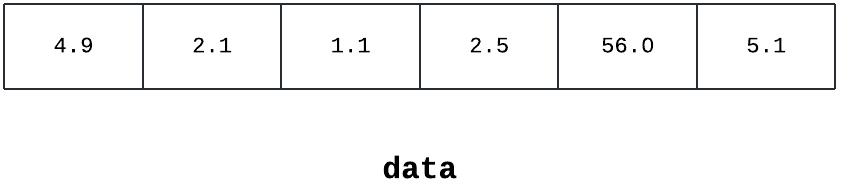
\includegraphics[width=0.7\linewidth]{images/03-Labs_vec} 

}

\caption{An illustration of a vector containing numeric values.}\label{fig:labs-vec}
\end{figure}

Within R, \textbf{vectors} are the simplest of the data structures and are one of the most commonly used to aid in the preparation and presentation of data. A vector is an ordered collection of values. They will store only objects of the same type. For instance, vectors are often used to store different colours to be used in a plot or other values that a variable can represent (this will be demonstrated in Chapter \ref{ch-4}).

Vectors are generally created using the \texttt{c} function:

\begin{Shaded}
\begin{Highlighting}[]
\CommentTok{\# a vector containing a collection of numbers }
\NormalTok{numbers }\OtherTok{\textless{}{-}} \FunctionTok{c}\NormalTok{(}\DecValTok{1}\NormalTok{, }\DecValTok{2}\NormalTok{, }\DecValTok{3}\NormalTok{, }\DecValTok{4}\NormalTok{)}

\CommentTok{\# display the vector}
\NormalTok{numbers}
\end{Highlighting}
\end{Shaded}

\begin{verbatim}
## [1] 1 2 3 4
\end{verbatim}

\begin{Shaded}
\begin{Highlighting}[]
\CommentTok{\# Find out the data class being stored within the vector}
\NormalTok{base}\SpecialCharTok{::}\FunctionTok{typeof}\NormalTok{(numbers)}
\end{Highlighting}
\end{Shaded}

\begin{verbatim}
## [1] "double"
\end{verbatim}

As mentioned above, a vector can contain only one type of data. If more than one type is supplied, R will try to coerce, i.e., convert, the lower-level, more specific, data types (e.g., logical) to a higher-order, more general type (e.g., characters) so that the function will work. Use the \texttt{typeof} function to check the data class of an object.

What happens when numbers and characters are forced into the same vector?

\begin{Shaded}
\begin{Highlighting}[]
\CommentTok{\# A factor containing different data types, where 1 and 3 are integers}
\CommentTok{\# and "two" and "four" are characters.}
\NormalTok{numbers }\OtherTok{\textless{}{-}} \FunctionTok{c}\NormalTok{(}\DecValTok{1}\NormalTok{, }\StringTok{"two"}\NormalTok{, }\DecValTok{3}\NormalTok{, }\StringTok{"four"}\NormalTok{)}

\CommentTok{\# Display the vector}
\NormalTok{numbers}
\end{Highlighting}
\end{Shaded}

\begin{verbatim}
## [1] "1"    "two"  "3"    "four"
\end{verbatim}

\begin{Shaded}
\begin{Highlighting}[]
\CommentTok{\# Find the data class that is stored within the vector}
\FunctionTok{class}\NormalTok{(numbers)}
\end{Highlighting}
\end{Shaded}

\begin{verbatim}
## [1] "character"
\end{verbatim}

R coerced the numbers into characters, as the characters can represent both types of data.

What would R coerce the following vectors into?
1. \texttt{x\ \textless{}-\ c(TRUE,\ 1,\ FALSE,\ 0)}
2. \texttt{x\ \textless{}-\ c(0,\ FALSE,\ "NO")}

\subsection{List}\label{sec:list}

\textbf{Lists} are one step up in complexity from vectors in that they are heterogeneous and, as such, can contain a variety of data types within a single list. However, like vectors, lists can store only one dimension of data, even though each element in a list can be completely different. It is also possible to create a list of lists.

Lists are created using the \texttt{list} function:

\begin{Shaded}
\begin{Highlighting}[]
\CommentTok{\# A list containing different data types, where 1 and 3 are numbers}
\CommentTok{\# and "two" and "four" are characters.}
\NormalTok{numbers }\OtherTok{\textless{}{-}} \FunctionTok{list}\NormalTok{(}\DecValTok{1}\NormalTok{, }\StringTok{"two"}\NormalTok{, }\DecValTok{3}\NormalTok{, }\StringTok{"four"}\NormalTok{)}

\CommentTok{\# Find out the data class being stored within the vector}
\NormalTok{utils}\SpecialCharTok{::}\FunctionTok{str}\NormalTok{(numbers)}
\end{Highlighting}
\end{Shaded}

\begin{verbatim}
## List of 4
##  $ : num 1
##  $ : chr "two"
##  $ : num 3
##  $ : chr "four"
\end{verbatim}

\subsection{Data Frames and Tibble}\label{sec:tibbleAnddataFrame}

\textbf{Tibbles} and \textbf{data frames} appear as tables within R. Like a list, data frames is a collection of a variety of data types. However, there are more restrictions on what can be put into a data frame because the data frame has to be `tabular' in nature (or rectangular in shape). Typically, a data frame is a collection of numeric (integer, double, etc.), string/factor, Boolean, or date/time vectors of the same length. Data are considered to be \textbf{tidy} when each \textbf{variable} has its own column and each \textbf{observation} (or case) has its own row.

\begin{figure}
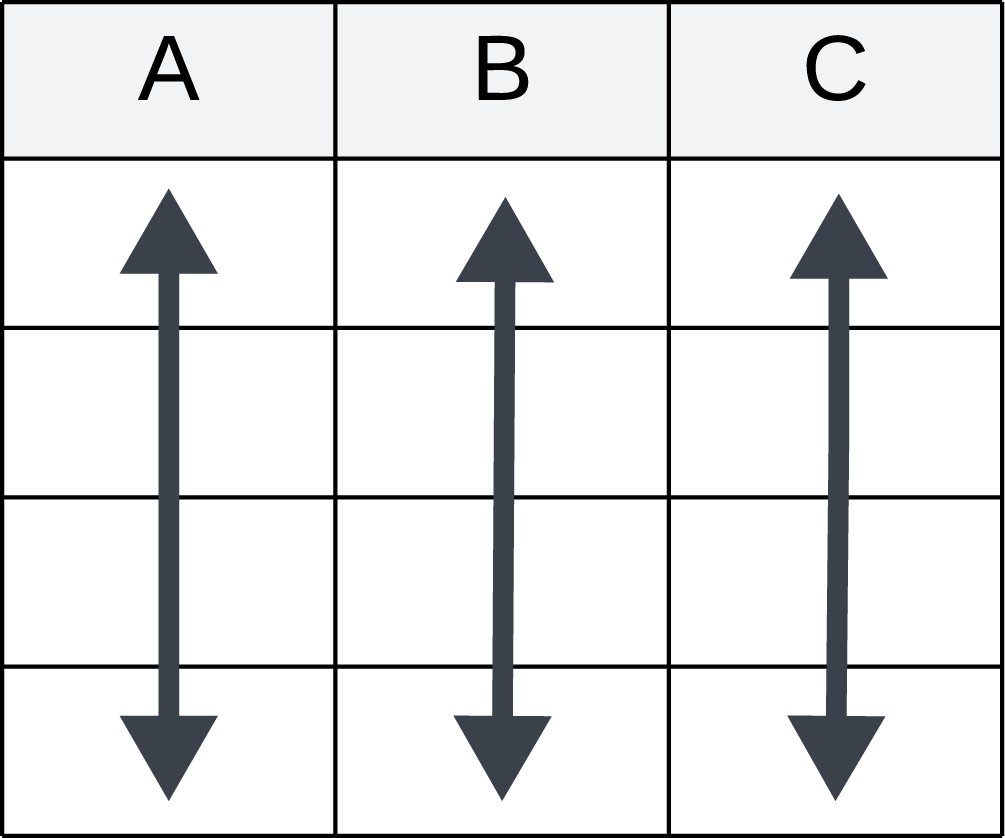
\includegraphics[width=0.49\linewidth]{images/03-Variables} 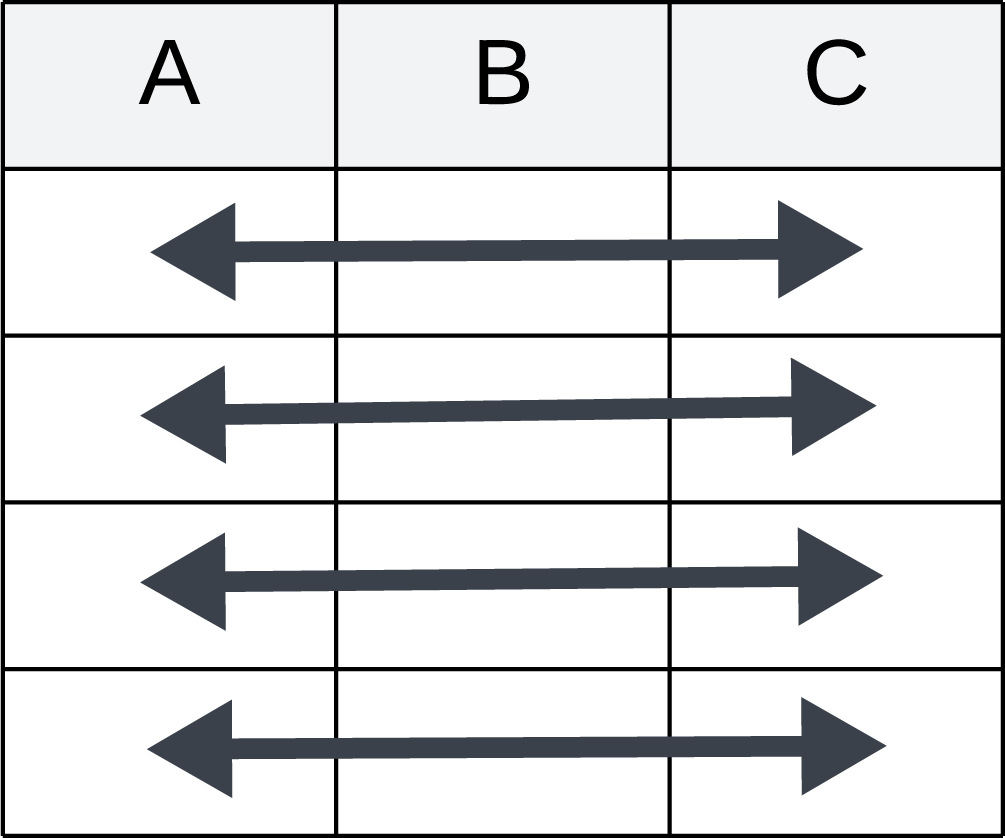
\includegraphics[width=0.49\linewidth]{images/03-Observations} \caption{A visual representation of tabular tidy data, where columns contain one variable and rows contain one observation or case.}\label{fig:dt-description}
\end{figure}

\subsubsection{Data Frame}\label{sec:dataFrame}

Data frames are constructed using \texttt{data.frame} by providing a sequence of vectors, one for each variable.

Example of how to build a data frame:

\begin{Shaded}
\begin{Highlighting}[]
\CommentTok{\# Specify the data frame}
\NormalTok{df }\OtherTok{\textless{}{-}}\NormalTok{ base}\SpecialCharTok{::}\FunctionTok{data.frame}\NormalTok{(}
   \AttributeTok{id =} \FunctionTok{c}\NormalTok{(}\DecValTok{5}\NormalTok{, }\DecValTok{14}\NormalTok{, }\DecValTok{16}\NormalTok{),}
   \AttributeTok{SampleDate =} \FunctionTok{c}\NormalTok{(}\FunctionTok{as.Date}\NormalTok{(}\StringTok{"2009{-}01{-}26"}\NormalTok{), }\FunctionTok{as.Date}\NormalTok{(}\StringTok{"2009{-}07{-}13"}\NormalTok{), }
           \FunctionTok{as.Date}\NormalTok{(}\StringTok{"2010{-}05{-}30"}\NormalTok{)),}
   \AttributeTok{Cr =} \FunctionTok{c}\NormalTok{(}\DecValTok{56}\NormalTok{, }\FloatTok{41.1}\NormalTok{, }\DecValTok{71}\NormalTok{)}
\NormalTok{)}

\CommentTok{\# examine the structure of the data frame.}
\NormalTok{utils}\SpecialCharTok{::}\FunctionTok{str}\NormalTok{(df)}
\end{Highlighting}
\end{Shaded}

\begin{verbatim}
## 'data.frame':    3 obs. of  3 variables:
##  $ id        : num  5 14 16
##  $ SampleDate: Date, format: "2009-01-26" "2009-07-13" ...
##  $ Cr        : num  56 41.1 71
\end{verbatim}

The function \texttt{nrow} can be used to get the number of rows (observations) in a data frame, while \texttt{ncol} can be used to get the number of columns (variables).

Try your hand at creating a data frame.

One important note: make sure to use \texttt{=} instead of \texttt{\textless{}-} when defining the variables of a data frame.

\subsubsection{Tibble}\label{sec:tibble}

\textbf{Tibbles} are tidyverse's modern take on R's \texttt{data.frame}, in that they have kept the most used features and have modified or dropped others. Of note, most of the tidyverse functions return tibble, while most other R packages take and return data frames. In an analogous grammar, a tibble is constructed using \texttt{tibble}, providing a sequence of vectors, one for each variable.

Example of how to build a tibble:

\begin{Shaded}
\begin{Highlighting}[]
\CommentTok{\# Specify the data frame}
\NormalTok{tib }\OtherTok{\textless{}{-}}\NormalTok{ tibble}\SpecialCharTok{::}\FunctionTok{tibble}\NormalTok{(}
   \AttributeTok{id =} \FunctionTok{c}\NormalTok{(}\DecValTok{5}\NormalTok{, }\DecValTok{14}\NormalTok{, }\DecValTok{16}\NormalTok{),}
   \AttributeTok{SampleDate =} \FunctionTok{c}\NormalTok{(}\FunctionTok{as.Date}\NormalTok{(}\StringTok{"2009{-}01{-}26"}\NormalTok{), }\FunctionTok{as.Date}\NormalTok{(}\StringTok{"2009{-}07{-}13"}\NormalTok{), }
           \FunctionTok{as.Date}\NormalTok{(}\StringTok{"2010{-}05{-}30"}\NormalTok{)),}
   \AttributeTok{Cr =} \FunctionTok{c}\NormalTok{(}\DecValTok{56}\NormalTok{, }\FloatTok{41.1}\NormalTok{, }\DecValTok{71}\NormalTok{)}
\NormalTok{)}

\CommentTok{\# examine the structure of the data frame.}
\NormalTok{utils}\SpecialCharTok{::}\FunctionTok{str}\NormalTok{(tib)}
\end{Highlighting}
\end{Shaded}

\begin{verbatim}
## tibble [3 x 3] (S3: tbl_df/tbl/data.frame)
##  $ id        : num [1:3] 5 14 16
##  $ SampleDate: Date[1:3], format: "2009-01-26" "2009-07-13" ...
##  $ Cr        : num [1:3] 56 41.1 71
\end{verbatim}

From the first line of the \texttt{str} output, \texttt{tib} object is a \texttt{tibble}, which extends the functionality of a \texttt{data.frame}.

Try creating a tibble using an analogous structure to the one created above.

\subsubsection{Tibble Versus Data frame}\label{sec:tibbleVsDataFrame}

In day-to-day use, it is not that important to know or focus on the differences between data frames and tibbles. Data frames can generally be converted to tibbles using \texttt{as\_tibble}.

Converting a data frame to a tibble using the tibble presented in Section \ref{sec:tibble}

\begin{Shaded}
\begin{Highlighting}[]
\FunctionTok{library}\NormalTok{(tibble)}
\NormalTok{df }\OtherTok{\textless{}{-}}\NormalTok{ base}\SpecialCharTok{::}\FunctionTok{data.frame}\NormalTok{(}
    \AttributeTok{id =} \FunctionTok{c}\NormalTok{(}\DecValTok{5}\NormalTok{, }\DecValTok{14}\NormalTok{, }\DecValTok{16}\NormalTok{),}
    \AttributeTok{SampleDate =} \FunctionTok{c}\NormalTok{(}\FunctionTok{as.Date}\NormalTok{(}\StringTok{"2009{-}01{-}26"}\NormalTok{), }\FunctionTok{as.Date}\NormalTok{(}\StringTok{"2009{-}07{-}13"}\NormalTok{), }
            \FunctionTok{as.Date}\NormalTok{(}\StringTok{"2010{-}05{-}30"}\NormalTok{)),}
    \AttributeTok{Cr =} \FunctionTok{c}\NormalTok{(}\DecValTok{56}\NormalTok{, }\FloatTok{41.1}\NormalTok{, }\DecValTok{71}\NormalTok{)}
\NormalTok{)}
\CommentTok{\# Data frame to tibble }
\NormalTok{utils}\SpecialCharTok{::}\FunctionTok{str}\NormalTok{(df)}
\end{Highlighting}
\end{Shaded}

\begin{verbatim}
## 'data.frame':    3 obs. of  3 variables:
##  $ id        : num  5 14 16
##  $ SampleDate: Date, format: "2009-01-26" "2009-07-13" ...
##  $ Cr        : num  56 41.1 71
\end{verbatim}

\begin{Shaded}
\begin{Highlighting}[]
\NormalTok{t }\OtherTok{\textless{}{-}}\NormalTok{ tibble}\SpecialCharTok{::}\FunctionTok{as\_tibble}\NormalTok{(df)}
\NormalTok{utils}\SpecialCharTok{::}\FunctionTok{str}\NormalTok{(t)}
\end{Highlighting}
\end{Shaded}

\begin{verbatim}
## tibble [3 x 3] (S3: tbl_df/tbl/data.frame)
##  $ id        : num [1:3] 5 14 16
##  $ SampleDate: Date[1:3], format: "2009-01-26" "2009-07-13" ...
##  $ Cr        : num [1:3] 56 41.1 71
\end{verbatim}

Tibbles can \textbf{always} be cast into data frames using \texttt{as.data.frame}.

Converting a tibble to a data frame using the data frame presented in Section \ref{sec:tibble}:

\begin{Shaded}
\begin{Highlighting}[]
\FunctionTok{library}\NormalTok{(tibble)}
\NormalTok{tib }\OtherTok{\textless{}{-}}\NormalTok{ tibble}\SpecialCharTok{::}\FunctionTok{tibble}\NormalTok{(}
    \AttributeTok{id =} \FunctionTok{c}\NormalTok{(}\DecValTok{5}\NormalTok{, }\DecValTok{14}\NormalTok{, }\DecValTok{16}\NormalTok{),}
    \AttributeTok{SampleDate =} \FunctionTok{c}\NormalTok{(}\FunctionTok{as.Date}\NormalTok{(}\StringTok{"2009{-}01{-}26"}\NormalTok{), }\FunctionTok{as.Date}\NormalTok{(}\StringTok{"2009{-}07{-}13"}\NormalTok{), }
            \FunctionTok{as.Date}\NormalTok{(}\StringTok{"2010{-}05{-}30"}\NormalTok{)),}
    \AttributeTok{Cr =} \FunctionTok{c}\NormalTok{(}\DecValTok{56}\NormalTok{, }\FloatTok{41.1}\NormalTok{, }\DecValTok{71}\NormalTok{)}
\NormalTok{)}
\CommentTok{\# Tibble to data frame}
\NormalTok{utils}\SpecialCharTok{::}\FunctionTok{str}\NormalTok{(tib)}
\end{Highlighting}
\end{Shaded}

\begin{verbatim}
## tibble [3 x 3] (S3: tbl_df/tbl/data.frame)
##  $ id        : num [1:3] 5 14 16
##  $ SampleDate: Date[1:3], format: "2009-01-26" "2009-07-13" ...
##  $ Cr        : num [1:3] 56 41.1 71
\end{verbatim}

\begin{Shaded}
\begin{Highlighting}[]
\NormalTok{df1 }\OtherTok{\textless{}{-}}\NormalTok{ base}\SpecialCharTok{::}\FunctionTok{as.data.frame}\NormalTok{(tib)}
\NormalTok{utils}\SpecialCharTok{::}\FunctionTok{str}\NormalTok{(df1)}
\end{Highlighting}
\end{Shaded}

\begin{verbatim}
## 'data.frame':    3 obs. of  3 variables:
##  $ id        : num  5 14 16
##  $ SampleDate: Date, format: "2009-01-26" "2009-07-13" ...
##  $ Cr        : num  56 41.1 71
\end{verbatim}

Visible in the two examples above, a benefit of tibbles is that their print function provides summary statistics, and it does not try to print the whole thing. That being said, almost every function that takes a tibble will also take a data frame, although the analogous is not true. If working within the tidyverse, consider the two interchangeable and focus on using tibbles as they are generally more user-friendly. However, when working outside of tidyverse, consider using data frames, as some packages and functions will only work with data frames.

\subsection{Factor}\label{sec:factor}

\textbf{Factors} are a data structure that should be used when dealing with categorical data (i.e., data that contain a finite number of distinct values, for example, biological sex or countries). Variables can be converted to factors using \texttt{as.factor} when the alphanumeric order of levels is desired (i.e., alphabetical order).

Example of converting a variable to a factor using \texttt{as.factor}:

\begin{Shaded}
\begin{Highlighting}[]
\CommentTok{\# Load in the demographic data}
\NormalTok{demog }\OtherTok{\textless{}{-}}\NormalTok{ utils}\SpecialCharTok{::}\FunctionTok{read.csv}\NormalTok{(}\StringTok{"data/03{-}diabetic\_demog.csv"}\NormalTok{)}

\CommentTok{\# Check the basic structure}
\NormalTok{utils}\SpecialCharTok{::}\FunctionTok{str}\NormalTok{(demog)}
\end{Highlighting}
\end{Shaded}

\begin{verbatim}
## 'data.frame':    197 obs. of  5 variables:
##  $ id    : int  5 14 16 25 29 46 49 56 61 71 ...
##  $ age   : int  28 12 9 9 13 12 8 12 16 21 ...
##  $ Gender: chr  "M" "M" "F" "M" ...
##  $ BMI   : int  26 23 30 28 36 20 28 35 33 38 ...
##  $ SIMD  : int  4 4 2 3 4 2 4 3 5 2 ...
\end{verbatim}

\begin{Shaded}
\begin{Highlighting}[]
\CommentTok{\# Convert gender to a factor}
\NormalTok{demog}\SpecialCharTok{$}\NormalTok{Gender }\OtherTok{\textless{}{-}}\NormalTok{ base}\SpecialCharTok{::}\FunctionTok{as.factor}\NormalTok{(demog}\SpecialCharTok{$}\NormalTok{Gender)}

\CommentTok{\# Check the structure again}
\NormalTok{utils}\SpecialCharTok{::}\FunctionTok{str}\NormalTok{(demog)}
\end{Highlighting}
\end{Shaded}

\begin{verbatim}
## 'data.frame':    197 obs. of  5 variables:
##  $ id    : int  5 14 16 25 29 46 49 56 61 71 ...
##  $ age   : int  28 12 9 9 13 12 8 12 16 21 ...
##  $ Gender: Factor w/ 2 levels "F","M": 2 2 1 2 2 1 1 2 1 2 ...
##  $ BMI   : int  26 23 30 28 36 20 28 35 33 38 ...
##  $ SIMD  : int  4 4 2 3 4 2 4 3 5 2 ...
\end{verbatim}

It is typically a vector or variable (column) in a data frame. In particular, it is important to ensure that ordinal data (data that have a natural rank order, e.g., quintiles of deprivation within \textbf{\hyperref[acronyms_SIMD]{SIMD}}) are converted into factors to prevent R from extrapolating values between individual levels, as R would do with continuous data,(e.g., keeping the order of 1, 2, 3, 4, and then 5 for the quintiles of \textbf{\hyperref[acronyms_SIMD]{SIMD}}, or reporting countries in alphabetical order).

Example of converting a variable to a factor using \texttt{as.factor}:

\begin{Shaded}
\begin{Highlighting}[]
\CommentTok{\# Load in the demographic data}
\NormalTok{demog }\OtherTok{\textless{}{-}}\NormalTok{ utils}\SpecialCharTok{::}\FunctionTok{read.csv}\NormalTok{(}\StringTok{"data/03{-}diabetic\_demog.csv"}\NormalTok{)}

\CommentTok{\# Convert SIMD to a factor}
\NormalTok{demog}\SpecialCharTok{$}\NormalTok{SIMD }\OtherTok{\textless{}{-}}\NormalTok{ base}\SpecialCharTok{::}\FunctionTok{as.factor}\NormalTok{(demog}\SpecialCharTok{$}\NormalTok{SIMD)}

\CommentTok{\# Use summary() to check the order of the factor levels}
\NormalTok{base}\SpecialCharTok{::}\FunctionTok{summary}\NormalTok{(demog}\SpecialCharTok{$}\NormalTok{SIMD)}
\end{Highlighting}
\end{Shaded}

\begin{verbatim}
##  1  2  3  4  5 
## 34 42 36 50 35
\end{verbatim}

From the \texttt{summary} function call, \textbf{\hyperref[acronyms_SIMD]{SIMD}} quintile 1 (the most deprived) has 34 individuals and is the first level of the \textbf{\hyperref[acronyms_SIMD]{SIMD}} factor. To flip the order, \texttt{factor} can be used to order and/or rename levels within a factor, where desired.

Example of converting a variable to a factor using \texttt{factor} to add some additional information and specify the order of the levels:

\begin{Shaded}
\begin{Highlighting}[]
\CommentTok{\# Load in the demographic data}
\NormalTok{demog }\OtherTok{\textless{}{-}}\NormalTok{ utils}\SpecialCharTok{::}\FunctionTok{read.csv}\NormalTok{(}\StringTok{"data/03{-}diabetic\_demog.csv"}\NormalTok{)}

\CommentTok{\# Convert SIMD to a factor}
\NormalTok{demog}\SpecialCharTok{$}\NormalTok{SIMD }\OtherTok{\textless{}{-}}\NormalTok{ base}\SpecialCharTok{::}\FunctionTok{factor}\NormalTok{(demog}\SpecialCharTok{$}\NormalTok{SIMD, }
                            \AttributeTok{levels =} \FunctionTok{c}\NormalTok{(}\DecValTok{5}\NormalTok{, }\DecValTok{4}\NormalTok{, }\DecValTok{3}\NormalTok{, }\DecValTok{2}\NormalTok{, }\DecValTok{1}\NormalTok{), }
                            \AttributeTok{labels =} \FunctionTok{c}\NormalTok{(}\StringTok{"5 (least deprived)"}\NormalTok{, }\StringTok{"4"}\NormalTok{, }\StringTok{"3"}\NormalTok{, }\StringTok{"2"}\NormalTok{, }
                            \StringTok{"1 (most deprived)"}\NormalTok{)}
\NormalTok{                        )}

\CommentTok{\# Use base::summary() to check the order of the factor levels}
\NormalTok{base}\SpecialCharTok{::}\FunctionTok{summary}\NormalTok{(demog}\SpecialCharTok{$}\NormalTok{SIMD)}
\end{Highlighting}
\end{Shaded}

\begin{verbatim}
## 5 (least deprived)                  4                  3                  2 
##                 35                 50                 36                 42 
##  1 (most deprived) 
##                 34
\end{verbatim}

In addition to being useful for statistics, factors are also more memory-efficient than storing information as a character string.

The impact of converting fields from character strings to factors:

\begin{Shaded}
\begin{Highlighting}[]
\FunctionTok{data}\NormalTok{(}\StringTok{"who"}\NormalTok{)}

\CommentTok{\# Get a summary of the country variable (the first column) }
\CommentTok{\# in the \textquotesingle{}who\textquotesingle{} dataset}
\FunctionTok{summary}\NormalTok{(who}\SpecialCharTok{$}\NormalTok{country)}
\end{Highlighting}
\end{Shaded}

\begin{verbatim}
##    Length     Class      Mode 
##      7240 character character
\end{verbatim}

\begin{Shaded}
\begin{Highlighting}[]
\CommentTok{\# Get the initial size of the country field within the dataset}
\FunctionTok{format}\NormalTok{(}\FunctionTok{object.size}\NormalTok{(who}\SpecialCharTok{$}\NormalTok{country), }\AttributeTok{unit =} \StringTok{\textquotesingle{}auto\textquotesingle{}}\NormalTok{)}
\end{Highlighting}
\end{Shaded}

\begin{verbatim}
## [1] "70.3 Kb"
\end{verbatim}

From the results of the \texttt{summary} call, it is possible to see that there are 7,240 records within the \texttt{country} field and that the field contains character strings, as denoted by \texttt{Class\ character}. That, at the moment, provides information on the number of records (\texttt{Length} as \texttt{7240}), but much more beyond that.

Now convert the country field to a factor and observe how the amount of memory needed to store it changes:

\begin{Shaded}
\begin{Highlighting}[]
\CommentTok{\# Load data}
\NormalTok{utils}\SpecialCharTok{::}\FunctionTok{data}\NormalTok{(}\StringTok{"who"}\NormalTok{)}

\CommentTok{\# Convert the country field to a factor}
\NormalTok{who}\SpecialCharTok{$}\NormalTok{country }\OtherTok{\textless{}{-}} \FunctionTok{as.factor}\NormalTok{(who}\SpecialCharTok{$}\NormalTok{country)}

\CommentTok{\# Rerun the first five levels of the \textquotesingle{}country\textquotesingle{} field }
\NormalTok{base}\SpecialCharTok{::}\FunctionTok{summary}\NormalTok{(who}\SpecialCharTok{$}\NormalTok{country, }\AttributeTok{maxsum =} \DecValTok{5}\NormalTok{)}
\end{Highlighting}
\end{Shaded}

\begin{verbatim}
##    Afghanistan        Albania        Algeria American Samoa        (Other) 
##             34             34             34             34           7104
\end{verbatim}

\begin{Shaded}
\begin{Highlighting}[]
\CommentTok{\# Check the new size of the \textquotesingle{}who\textquotesingle{} dataset}
\FunctionTok{format}\NormalTok{(}\FunctionTok{object.size}\NormalTok{(who}\SpecialCharTok{$}\NormalTok{country), }\AttributeTok{unit =} \StringTok{\textquotesingle{}auto\textquotesingle{}}\NormalTok{)}
\end{Highlighting}
\end{Shaded}

\begin{verbatim}
## [1] "44.1 Kb"
\end{verbatim}

Converting \texttt{country} reduced the amount of memory needed to store that field by just over half. Additionally, the \texttt{summary} function now provides a more meaningful result.

How memory-efficient can you make the \texttt{who} dataset in three minutes? Which columns did you change, to what, and why?

\subsection{Array}\label{sec:array}

Compared to the other data structures mentioned in Sections \ref{sec:vector} through \ref{sec:dataFrame}, \textbf{arrays} can have varying dimensions, often more than two, but must contain the same type of data. Arrays are created using \texttt{array}, which takes the data first, and then the dimensions through the \texttt{dim\ =}, as parameters.

Examples of creating arrays:

\begin{Shaded}
\begin{Highlighting}[]
\CommentTok{\# An example of a 2D array}
\NormalTok{my\_2d\_array }\OtherTok{\textless{}{-}}\NormalTok{ base}\SpecialCharTok{::}\FunctionTok{array}\NormalTok{(}\DecValTok{1}\SpecialCharTok{:}\DecValTok{12}\NormalTok{, }\AttributeTok{dim =} \FunctionTok{c}\NormalTok{(}\DecValTok{3}\NormalTok{, }\DecValTok{4}\NormalTok{))  }
\NormalTok{base}\SpecialCharTok{::}\FunctionTok{print}\NormalTok{(my\_2d\_array)}
\end{Highlighting}
\end{Shaded}

\begin{verbatim}
##      [,1] [,2] [,3] [,4]
## [1,]    1    4    7   10
## [2,]    2    5    8   11
## [3,]    3    6    9   12
\end{verbatim}

\begin{Shaded}
\begin{Highlighting}[]
\CommentTok{\# An example of a 3D array }
\NormalTok{my\_3d\_array }\OtherTok{\textless{}{-}}\NormalTok{ base}\SpecialCharTok{::}\FunctionTok{array}\NormalTok{(}\DecValTok{1}\SpecialCharTok{:}\DecValTok{24}\NormalTok{, }\AttributeTok{dim =} \FunctionTok{c}\NormalTok{(}\DecValTok{3}\NormalTok{, }\DecValTok{4}\NormalTok{, }\DecValTok{2}\NormalTok{))}
\NormalTok{base}\SpecialCharTok{::}\FunctionTok{print}\NormalTok{(my\_3d\_array)}
\end{Highlighting}
\end{Shaded}

\begin{verbatim}
## , , 1
## 
##      [,1] [,2] [,3] [,4]
## [1,]    1    4    7   10
## [2,]    2    5    8   11
## [3,]    3    6    9   12
## 
## , , 2
## 
##      [,1] [,2] [,3] [,4]
## [1,]   13   16   19   22
## [2,]   14   17   20   23
## [3,]   15   18   21   24
\end{verbatim}

The first example above is similar to a matrix, data frame, or tibble. The second example illustrates the n-dimensionality that arrays allow. In addition to \texttt{str}, \texttt{nrow} and \texttt{ncol} can be used to retrieve individual dimensions.

\subsection{Others}\label{sec:OtherDataTypes}

A few other types of data structures that are less commonly used include matrices, \texttt{data.table}, and custom objects. \textbf{Matrices} are effectively the matrices of linear algebra and, as such, are often used to represent the data used in mathematical models. Their functionality is provided in base R. Matrices are two-dimensional data structures, similar to data frames. However, unlike data frames, all elements of a matrix need to be of the same data type.

The \textbf{data.table} data structure is provided through the \texttt{data.table} package and provides an enhanced version of data frames for working with larger data sets or where speeding up computational time is desired. Check out \url{https://cran.r-project.org/web/packages/data.table/vignettes/datatable-intro.html} for further information.

Ultimately, sometimes the standard data structures just don't quite fulfil all of the requirements. If this is the case, consider whether the code and data requirements can be restructured to use one of the previously mentioned data structures. If restructuring does not work, this is the point of jumping off into the deeper end of defining \textbf{custom object} classes using \textbf{object-oriented programming} becomes a consideration. This is beyond the scope of the course, but additional information can be found here:

\begin{itemize}
\tightlist
\item
  \url{https://adv-r.hadley.nz/oo.html}
\item
  \url{https://stat.ethz.ch/R-manual/R-devel/library/methods/html/setClass.html}
\end{itemize}

\section{Statistical Data Types}\label{statistical-data-types}

Now that the computational aspects of defining data types and their containers have been covered, this section will cover the statistical aspects of the same topic. From the statistical side, the main types of statistical data that will be used or modelled are nominal, ordinal, interval, and ratio. Each of the four statistical data types provides different kinds of information and requires different interpretations.

\begin{figure}

{\centering 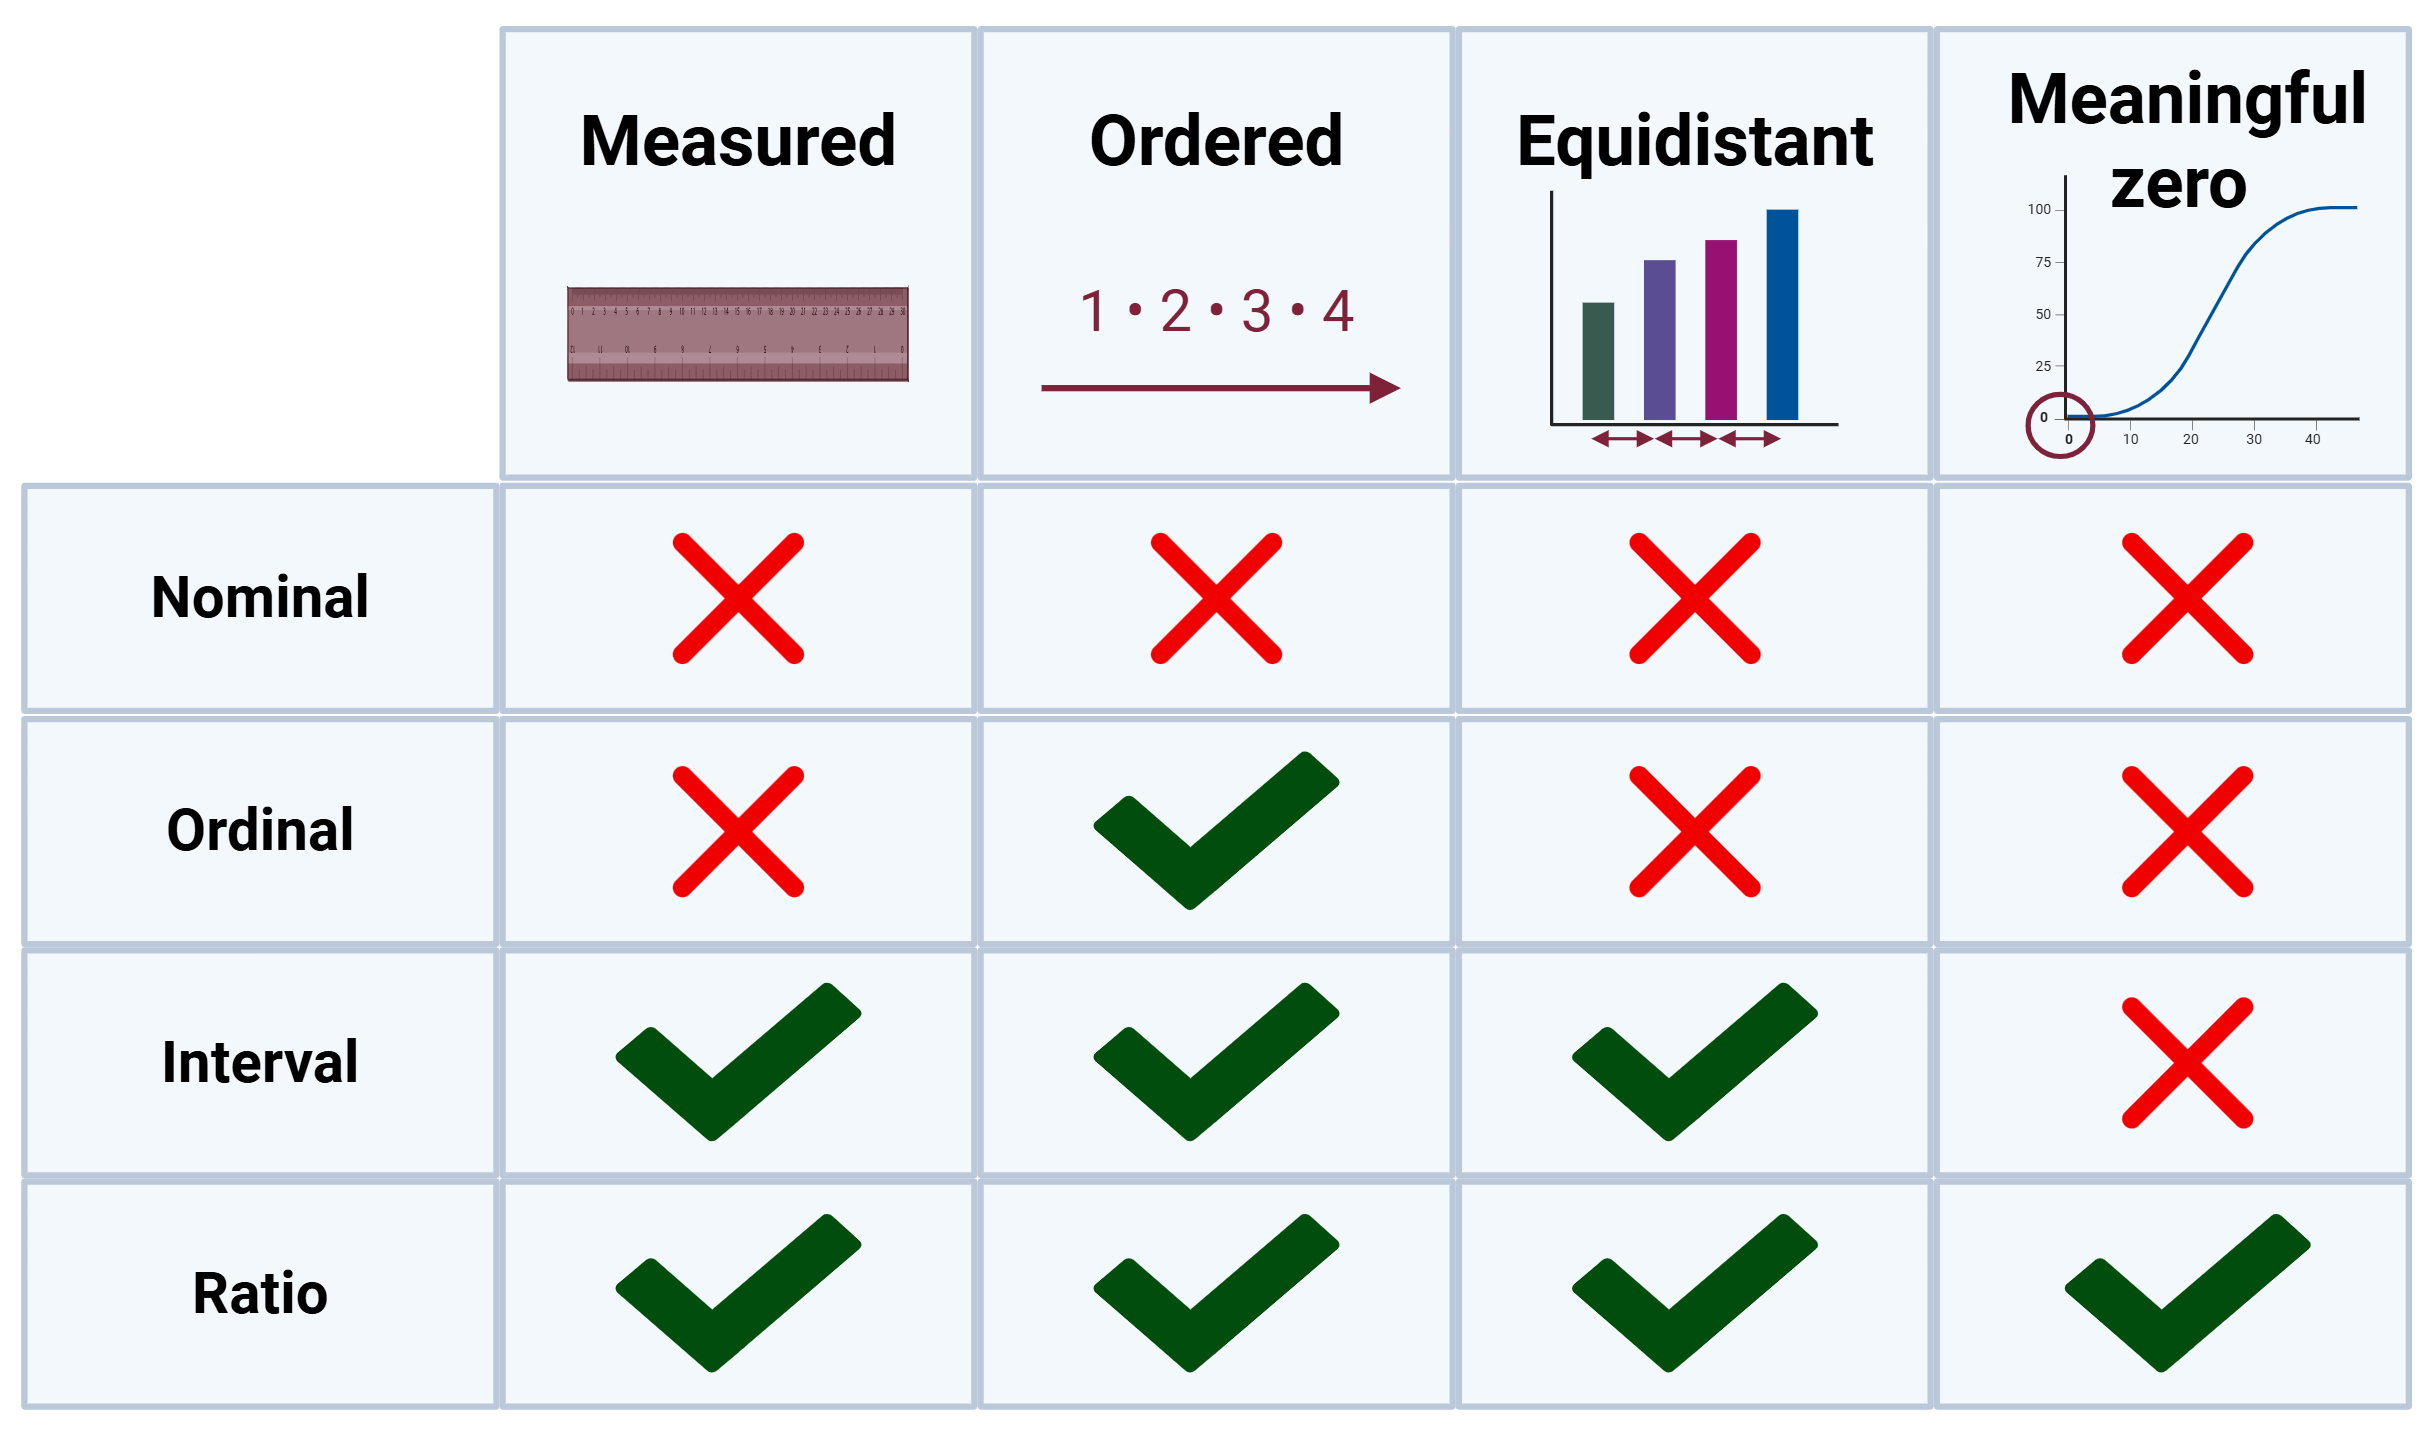
\includegraphics[width=0.8\linewidth]{images/03-Statistical data types} 

}

\caption{An illustration of differences and commonalities between statistical data types.}\label{fig:stat-data-types}
\end{figure}

\subsection{Nominal Data}\label{sec:nominal}

Starting from the simplest form, \textbf{nominal data} are defined as the data used to name (hence nominal borrowing from the Latin version for concerned with names). As illustrated in Figure \ref{fig:stat-data-types}, nominal data are data such as patient ID, nationality, ethnicity, or name that are used to identify objects or events. The numbers do not have an order, implying that one value is not superior to another; nor is a zero meaningful; nominal data classifies objects. Use factors (see Section \ref{sec:factor}) when dealing with nominal data. \textbf{Dichotomous data} are a subtype of nominal data that have only two categories. Examples for this include death status (alive versus dead) or sex (men versus women).

\subsection{Ordinal Data}\label{sec:ordinal}

In contrast to nominal data, \textbf{ordinal data} have an inherent order but do not provide an amount or a degree of quality. Often, one means that something is better or higher in rank than that in rank number 2, rank 2 is better or higher than rank 3, and so forth. Notably, the numerical difference between the levels can be arbitrary, and the levels do not need to differ by a fixed amount, unlike interval data. Both ordinal and nominal fall under the colloquial term of \textbf{categorical} data.

\subsection{Interval Data}\label{sec:interval}

\textbf{Interval data} are numerical data that have equal distances between adjacent values and no meaningful zero. There can be a finite number of intervals, where the data are organised into categories (\textbf{discrete}), or there can be an infinite number of intervals (\textbf{continuous}). Either way, the interval data must have an equal space between the different values, and hence the `interval' in the interval data. Examples of interval data include dates (e.g., 2022, 2023) or times (e.g., 5 am, 5 pm).

\subsection{Ratio Data}\label{sec:ratio}

\textbf{Ratio data} are data that are numeric, have equal distance between adjacent values (a commonality with interval data above), and have a meaningful zero, unlike the other numerical data types. Ratio data can either be \textbf{discrete} or \textbf{continuous}. The key point is that the ratio data must have a non-arbitrary zero value.

Can you come up with two examples for each statistical data type:
1. Nominal
2. Ordinal
3. Interval
4. Ratio

And how would you represent these in code?

\section{Tidyverse}\label{sec:tidyverse}

The \texttt{tidyverse} has become a powerhouse set of R packages designed to work seamlessly together to streamline the data science process and development of pipelines for data science. In short, within \texttt{tidyverse}, all packages share the same underlying design, philosophy, grammar, and data structures (e.g., tibbles from Section \ref{sec:tibble}). Some \texttt{tidyverse} packages have already been introduced, such as \texttt{lubridate} in Section \ref{sec:datesAndTimes}.

Further reading:
* The main textbook: \url{https://r4ds.hadley.nz/}
* The history of Tidyverse: \url{https://hadley.github.io/25-tidyverse-history/}

\subsection{Piping}\label{sec:piping}

One of the big innovations that came with \texttt{magrittr}, an integral part of tidyverse, is \textbf{piping}. In plain English, pipes work by `taking \emph{this} object, passing it to a function to do something, and then potentially passing it to another function, and so on.' Instead of nesting functions, the pipe allows the result of each step to be passed to the next function using \texttt{\%\textgreater{}\%} (or the newer \texttt{\textbar{}\textgreater{}} in base R).

Example of piping data:

\begin{Shaded}
\begin{Highlighting}[]
\CommentTok{\# Define a vector of data }
\NormalTok{data }\OtherTok{\textless{}{-}} \FunctionTok{c}\NormalTok{(}\DecValTok{1}\NormalTok{, }\DecValTok{2}\NormalTok{, }\DecValTok{5}\NormalTok{, }\DecValTok{7}\NormalTok{)}

\CommentTok{\# finding the mean without using pipes}
\NormalTok{base}\SpecialCharTok{::}\FunctionTok{mean}\NormalTok{(data)}
\end{Highlighting}
\end{Shaded}

\begin{verbatim}
## [1] 3.75
\end{verbatim}

\begin{Shaded}
\begin{Highlighting}[]
\CommentTok{\# finding the mean while using pipes}
\NormalTok{data }\SpecialCharTok{|\textgreater{}}\NormalTok{ base}\SpecialCharTok{::}\FunctionTok{mean}\NormalTok{()}
\end{Highlighting}
\end{Shaded}

\begin{verbatim}
## [1] 3.75
\end{verbatim}

Pipes mean that data are carried forward and don't need to be re-included as the first argument to a function; however, if data needs to be passed in as somewhere other than the first argument, use \texttt{.} as a placeholder.

Example of piping data:

\begin{Shaded}
\begin{Highlighting}[]
\CommentTok{\# Where the data are the first argument}
\NormalTok{data }\SpecialCharTok{\%\textgreater{}\%} \FunctionTok{some\_function}\NormalTok{(argument1, agument1, ...)}

\CommentTok{\# Where the data need to be the second argument }
\NormalTok{data }\SpecialCharTok{\%\textgreater{}\%} \FunctionTok{some\_function}\NormalTok{(argument1, }\AttributeTok{data =}\NormalTok{ .)}
\end{Highlighting}
\end{Shaded}

Piping can be a useful way to write easy-to-understand code as it avoids nesting or multiple, repeated simple operations. It also shows the operations step by step. More examples will be shown below of how piping can make code more readable. Generally speaking, the goal is to write R code so that it is as readable as possible for two reasons: (1) it allows others to understand it more easily, and (2) it minimises human errors in coding.

\subsection{Tidy Data}\label{sec:tidyData}

The philosophy for tidy data was developed around avoiding the Anna Karenina principle, which comes from the first line of Tolstoy's \emph{Anna Karenina}, ``All happy families are alike; each unhappy family is unhappy in its own way''. This is evidenced by the quote from Hadley Wickham, the leader of the tidyverse team, ``Tidy datasets are all alike, but every messy dataset is messy in its own way''. This drives the tidyverse definition of \textbf{tidy data}. Within the tidyverse, and general good practice in R, tidy data frames and tibbles follow the following three rules:

\begin{enumerate}
\def\labelenumi{\arabic{enumi}.}
\tightlist
\item
  Each variable is a column, and each column is a variable;
\item
  Each observation is a row, and each row is an observation;
\item
  And each value is a cell, and each cell is a single value.
\end{enumerate}

The value of using tidy data is that picking one consistent way to store data means that it's easier to learn new tools and take advantage of R's vectorised nature. It's also handy that all packages in the tidyverse are designed to work with tidy data.

\subsubsection{Wide Versus Long Data}\label{sec:wideLong}

To date, most of the data that has been presented are in what is called \textbf{wide format}, where each participant/entity has one row per table and multiple columns of values. In the case of the lab data, each sample at a given time has multiple test results; although some patients have multiple samples, this is still considered wide data. The inverse of this is called \textbf{long data}, where the participant/entity has multiple rows, and with the type of record recorded as a variable.

\begin{figure}
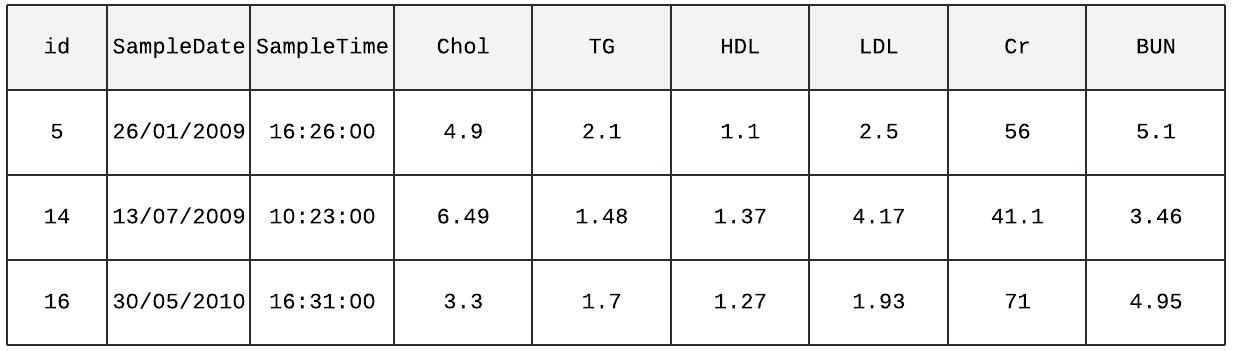
\includegraphics[width=0.49\linewidth]{images/03-WideData} 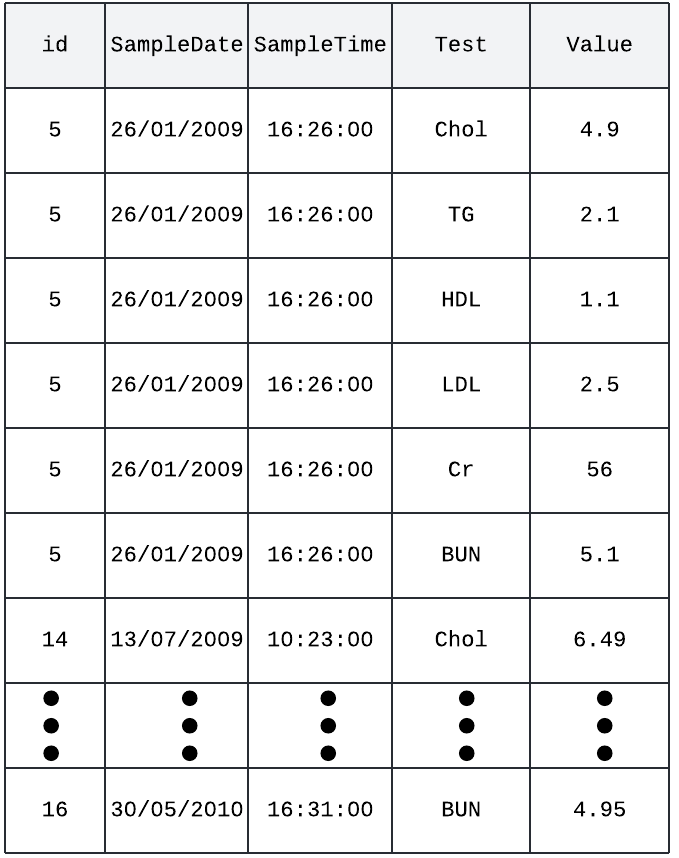
\includegraphics[width=0.49\linewidth]{images/03-LongData} \caption{A visual representation of wide versus long data, in wide data, each row contains multiple measurements, versus in long data, where each row contains one measurement.}\label{fig:wide-v-long}
\end{figure}

The wide format data are easier for reading, while the long format data are typically easier for analysis and data visualisation.

\subsubsection{Pivoting Data}\label{sec:pivotingData}

Data frames and tibbles can easily be converted from wide to long and vice versa through \textbf{pivoting}. The term \textbf{pivot} comes from the idea of a pivot table implemented in spreadsheets, where a pivot table rotates data so that they can be viewed from different angles. The phrase \textbf{pivot longer} means taking columns/variables and rotating them \emph{downwards} into rows/observations. This can be done using \texttt{pivot\_longer} from the \texttt{tidyr} package.

Convert from wide to long format:

\begin{Shaded}
\begin{Highlighting}[]
\FunctionTok{library}\NormalTok{(tidyr)}
    
\NormalTok{wide\_lab }\OtherTok{\textless{}{-}}\NormalTok{ utils}\SpecialCharTok{::}\FunctionTok{read.csv}\NormalTok{(}\StringTok{"data/03{-}diabetic\_labs\_final\_with\_missing.csv"}\NormalTok{, }\AttributeTok{head =} \ConstantTok{TRUE}\NormalTok{)}

\CommentTok{\#pivot around id, SampleDate and SampleTime}
\NormalTok{long\_data }\OtherTok{\textless{}{-}}\NormalTok{ wide\_lab }\SpecialCharTok{\%\textgreater{}\%}\NormalTok{ tidyr}\SpecialCharTok{::}\FunctionTok{pivot\_longer}\NormalTok{(}
    \CommentTok{\# columns to pivot}
    \AttributeTok{cols =} \FunctionTok{c}\NormalTok{(}\StringTok{"Chol"}\NormalTok{, }\StringTok{"TG"}\NormalTok{, }\StringTok{"HDL"}\NormalTok{, }\StringTok{"LDL"}\NormalTok{, }\StringTok{"Cr"}\NormalTok{, }\StringTok{"BUN"}\NormalTok{), }
    \CommentTok{\# new column name for old headers}
    \AttributeTok{names\_to =} \StringTok{"Test"}\NormalTok{, }
    \CommentTok{\# new column name for values }
    \AttributeTok{values\_to =} \StringTok{"Value"}
\NormalTok{)}

\FunctionTok{head}\NormalTok{(long\_data, }\AttributeTok{n=}\DecValTok{5}\NormalTok{)}
\end{Highlighting}
\end{Shaded}

\begin{verbatim}
## # A tibble: 5 x 5
##      id SampleDate SampleTime Test  Value
##   <int> <chr>      <chr>      <chr> <dbl>
## 1     5 26/01/2009 16:26:00   Chol    4.9
## 2     5 26/01/2009 16:26:00   TG      2.1
## 3     5 26/01/2009 16:26:00   HDL     1.1
## 4     5 26/01/2009 16:26:00   LDL     2.5
## 5     5 26/01/2009 16:26:00   Cr     56
\end{verbatim}

The phrase \textbf{pivot wider} means taking rows/observations and rotating them \emph{outwards} into columns/variables. This can be done using \texttt{pivot\_wider} from the \texttt{tidyr} package.

Convert from long to wide format:

\begin{Shaded}
\begin{Highlighting}[]
\CommentTok{\#pivot around id, SampleDate and SampleTime}
\NormalTok{wide\_data }\OtherTok{\textless{}{-}}\NormalTok{ long\_data }\SpecialCharTok{\%\textgreater{}\%}\NormalTok{ tidyr}\SpecialCharTok{::}\FunctionTok{pivot\_wider}\NormalTok{(}
    \CommentTok{\# new column name for old headers}
    \AttributeTok{names\_from =} \StringTok{"Test"}\NormalTok{, }
    \CommentTok{\# values in this column fill the cells}
    \AttributeTok{values\_from =} \StringTok{"Value"}
\NormalTok{)}

\FunctionTok{head}\NormalTok{(wide\_data, }\AttributeTok{n=}\DecValTok{5}\NormalTok{)}
\end{Highlighting}
\end{Shaded}

\begin{verbatim}
## # A tibble: 5 x 9
##      id SampleDate SampleTime  Chol    TG   HDL   LDL    Cr   BUN
##   <int> <chr>      <chr>      <dbl> <dbl> <dbl> <dbl> <dbl> <dbl>
## 1     5 26/01/2009 16:26:00    4.9   2.1   1.1   2.5   56    5.1 
## 2     5 19/10/2012 10:22:00    3.6   5.1   0.9   2.5   63    5   
## 3     5 19/10/2012 09:31:00    4.85  1.63  4.86  4.86  96.7  5.24
## 4    14 13/07/2009 10:23:00    6.49  1.48  1.37  4.17  41.1  3.46
## 5    14 07/10/2010 11:05:00   NA     0.92  4.86  4.86  60    4.72
\end{verbatim}

The use of a long versus a wide data format depends on the specific analysis or operation required. Typically, most analyses require wide-format data; however, in cases where data have repeated measures, long-format data may be more suitable, as many mixed models require this format. In addition, \texttt{ggplot2} often requires that data are summarised in a long format. More about that will be covered in Chapter \ref{ch-4}.

\section{Data Transformation}\label{sec:dataTransformation}

Very rarely will a data set be presented as analysis-ready. Rather, the typical situation involves importing flat files that store records in a single table, followed by formatting (e.g., converting character strings of dates into Dates, nominal data into factors, and making sure that ordinal data are ordered correctly).

\subsection{Summaries}\label{sec:summary}

\textbf{Summaries} are a way to condense many values into fewer, essentially creating a concise overview of the data provided, hence the name. In general, this is done using the \texttt{summary} function, which has been used throughout previous sections. One of the benefits of working within an object-oriented programming environment is that \texttt{summary} can be applied to any object. However, each will have a different summary.

Try the following codes and see how R shows different output depending on the data type. Note that the iris dataset will be extensively used in Chapter \ref{ch-4} and the code used in Example 4 will be taught in Chapter \ref{ch-5}.
1. Whole dataset: \texttt{base::summary(demog)}
2. A series: \texttt{base::summary(1:5)}
3. A variable within a dataset: \texttt{base::summary(demog\$BMI)}
4. A function call: \texttt{base::summary(stats::lm(BMI\ \textasciitilde{}\ SIMD,\ data=demog))}

Ultimately, the base R version of creating summaries is more ad hoc. In contrast, \texttt{dplyr} provides a \texttt{summarise} function, which is often integrated into pipelines by providing summary statistics that can be used in figures or tables downstream.

Examples of dplyr's summarise function using the diabeticDemog dataset:

\begin{Shaded}
\begin{Highlighting}[]
\FunctionTok{library}\NormalTok{(dplyr)}
\NormalTok{demog }\OtherTok{\textless{}{-}}\NormalTok{ utils}\SpecialCharTok{::}\FunctionTok{read.csv}\NormalTok{(}\StringTok{"data/03{-}diabetic\_demog.csv"}\NormalTok{)}

\NormalTok{demog }\SpecialCharTok{\%\textgreater{}\%} 
    \CommentTok{\# define the minimum, mean, and maximum age}
\NormalTok{    dplyr}\SpecialCharTok{::}\FunctionTok{summarise}\NormalTok{(}
                \AttributeTok{mean\_age =} \FunctionTok{mean}\NormalTok{(age, }\AttributeTok{na.rm=}\ConstantTok{TRUE}\NormalTok{), }
                \AttributeTok{mim\_age =} \FunctionTok{min}\NormalTok{(age, }\AttributeTok{na.rm=}\ConstantTok{TRUE}\NormalTok{), }
                \AttributeTok{max\_age =} \FunctionTok{max}\NormalTok{(age, }\AttributeTok{na.rm=}\ConstantTok{TRUE}\NormalTok{)}
\NormalTok{            )}
\end{Highlighting}
\end{Shaded}

\begin{verbatim}
##   mean_age mim_age max_age
## 1 20.78173       1      58
\end{verbatim}

\subsection{Mutating}\label{sec:mutating}

Within R, the term \textbf{mutating} is used when new variables are added or existing variables are modified within data frames or tibbles. In short, it is used when an object is changed after its creation.

Using dplyr to add a variable:

\begin{Shaded}
\begin{Highlighting}[]
\CommentTok{\#define the data frame}
\NormalTok{df }\OtherTok{\textless{}{-}} \FunctionTok{data.frame}\NormalTok{(}\AttributeTok{id =} \FunctionTok{c}\NormalTok{(}\DecValTok{5}\NormalTok{, }\DecValTok{14}\NormalTok{, }\DecValTok{16}\NormalTok{), }
        \AttributeTok{SampleDate =} \FunctionTok{c}\NormalTok{(}\StringTok{"26{-}01{-}2009"}\NormalTok{, }\StringTok{"13{-}07{-}2009"}\NormalTok{, }\StringTok{"30{-}05{-}2010"}\NormalTok{), }
        \AttributeTok{SampleTime =} \FunctionTok{c}\NormalTok{(}\StringTok{"16:26:00"}\NormalTok{, }\StringTok{"10:23:00"}\NormalTok{, }\StringTok{"16:31:00"}\NormalTok{), }
        \AttributeTok{Chol =} \FunctionTok{c}\NormalTok{(}\FloatTok{4.9}\NormalTok{, }\FloatTok{6.49}\NormalTok{, }\FloatTok{3.3}\NormalTok{), }
        \AttributeTok{TG =} \FunctionTok{c}\NormalTok{(}\FloatTok{2.1}\NormalTok{, }\FloatTok{1.48}\NormalTok{, }\FloatTok{1.7}\NormalTok{), }
        \AttributeTok{HDL =} \FunctionTok{c}\NormalTok{(}\FloatTok{1.1}\NormalTok{, }\FloatTok{1.37}\NormalTok{, }\FloatTok{1.27}\NormalTok{), }
        \AttributeTok{LDL =} \FunctionTok{c}\NormalTok{(}\FloatTok{2.5}\NormalTok{, }\FloatTok{4.14}\NormalTok{, }\FloatTok{1.93}\NormalTok{),  }
        \AttributeTok{Cr =} \FunctionTok{c}\NormalTok{(}\FloatTok{56.0}\NormalTok{, }\FloatTok{41.1}\NormalTok{, }\DecValTok{71}\NormalTok{),}
        \AttributeTok{BUN =} \FunctionTok{c}\NormalTok{(}\FloatTok{5.1}\NormalTok{, }\FloatTok{3.46}\NormalTok{, }\FloatTok{4.95}\NormalTok{))}

\FunctionTok{library}\NormalTok{(dplyr)}
\CommentTok{\# Creating a new column}
\NormalTok{df }\OtherTok{\textless{}{-}}\NormalTok{ df }\SpecialCharTok{\%\textgreater{}\%}\NormalTok{ dplyr}\SpecialCharTok{::}\FunctionTok{mutate}\NormalTok{(}\AttributeTok{HDL\_mgdL =}\NormalTok{ HDL}\SpecialCharTok{/}\FloatTok{38.67}\NormalTok{)}
\FunctionTok{head}\NormalTok{(df, }\DecValTok{2}\NormalTok{)}
\end{Highlighting}
\end{Shaded}

\begin{verbatim}
##   id SampleDate SampleTime Chol   TG  HDL  LDL   Cr  BUN   HDL_mgdL
## 1  5 26-01-2009   16:26:00 4.90 2.10 1.10 2.50 56.0 5.10 0.02844582
## 2 14 13-07-2009   10:23:00 6.49 1.48 1.37 4.14 41.1 3.46 0.03542798
\end{verbatim}

\begin{Shaded}
\begin{Highlighting}[]
\CommentTok{\# Modifying a column}
\NormalTok{df}\OtherTok{\textless{}{-}}\NormalTok{ df }\SpecialCharTok{\%\textgreater{}\%}\NormalTok{ dplyr}\SpecialCharTok{::}\FunctionTok{mutate}\NormalTok{(}\AttributeTok{HDL\_mgdL =}\NormalTok{ HDL\_mgdL}\SpecialCharTok{*}\DecValTok{10}\NormalTok{)}
\FunctionTok{head}\NormalTok{(df, }\DecValTok{2}\NormalTok{)}
\end{Highlighting}
\end{Shaded}

\begin{verbatim}
##   id SampleDate SampleTime Chol   TG  HDL  LDL   Cr  BUN  HDL_mgdL
## 1  5 26-01-2009   16:26:00 4.90 2.10 1.10 2.50 56.0 5.10 0.2844582
## 2 14 13-07-2009   10:23:00 6.49 1.48 1.37 4.14 41.1 3.46 0.3542798
\end{verbatim}

In the above code, both the original (\texttt{**\textbackslash{}acr\{HDL\}**}) and new (\texttt{HDL\_mgdL}) variables remain in the data frame. The \texttt{mutate} function provides the ability to keep or drop variables by specifying the desired functionality using the \texttt{.keep} parameter. The default option is \texttt{.keep\ =\ "all"} where all variables, both used and unused, are kept. The \texttt{none} option only keeps the new variable; the \texttt{used} option only keeps the new variable and the variables used to create it; and the \texttt{unused} option keeps the result and drops the variables used to create the new variable.

Using dplyr to add a variable with \texttt{.keep}:

\begin{Shaded}
\begin{Highlighting}[]
\CommentTok{\# Creating a new column }
\NormalTok{df }\OtherTok{\textless{}{-}}\NormalTok{ df }\SpecialCharTok{\%\textgreater{}\%}\NormalTok{ dplyr}\SpecialCharTok{::}\FunctionTok{mutate}\NormalTok{(}\AttributeTok{HDL\_mgdL\_new =}\NormalTok{ HDL}\SpecialCharTok{/}\FloatTok{38.67}\NormalTok{, }\AttributeTok{.keep =} \StringTok{"unused"}\NormalTok{)}
\FunctionTok{head}\NormalTok{(df, }\DecValTok{2}\NormalTok{)}
\end{Highlighting}
\end{Shaded}

\begin{verbatim}
##   id SampleDate SampleTime Chol   TG  LDL   Cr  BUN  HDL_mgdL HDL_mgdL_new
## 1  5 26-01-2009   16:26:00 4.90 2.10 2.50 56.0 5.10 0.2844582   0.02844582
## 2 14 13-07-2009   10:23:00 6.49 1.48 4.14 41.1 3.46 0.3542798   0.03542798
\end{verbatim}

Of note, when first developing code, it is best to keep all variables so that the logic and execution of the new variable can be sense checked.

Using the DiabeticLabs\_final\_withMissing.csv and DiabeticDemog.csv, experiment with creating different variables and changing the \texttt{.keep} parameter.

\subsection{Grouping and Ungrouping}\label{sec:groupingUnGrouping}

Intuitively, \textbf{grouping} is a way of splitting data into smaller chunks based on values of one or more variables for the purpose of applying operations or functions (e.g., finding the mean, minimum, maximum, etc.) to each group of data. In base R, grouping is temporary and tied to the function call by being passed as an argument each time, so the groups only exist inside the function call.

Grouping examples using dplyr:

\begin{Shaded}
\begin{Highlighting}[]
\FunctionTok{library}\NormalTok{(dplyr)}
\NormalTok{lab\_data }\OtherTok{\textless{}{-}}\NormalTok{ utils}\SpecialCharTok{::}\FunctionTok{read.csv}\NormalTok{(}\StringTok{"data/03{-}diabetic\_labs\_final\_with\_missing.csv"}\NormalTok{, }\AttributeTok{head =} \ConstantTok{TRUE}\NormalTok{)}

\CommentTok{\# Example using dplyr::group\_by()}
\NormalTok{lab\_data }\SpecialCharTok{\%\textgreater{}\%} 
\NormalTok{    dplyr}\SpecialCharTok{::}\FunctionTok{group\_by}\NormalTok{(id) }\SpecialCharTok{\%\textgreater{}\%} 
\NormalTok{    dplyr}\SpecialCharTok{::}\FunctionTok{summarise}\NormalTok{(}\AttributeTok{mean\_chol =} \FunctionTok{mean}\NormalTok{(Chol)) }\SpecialCharTok{\%\textgreater{}\%}
    \FunctionTok{head}\NormalTok{(}\DecValTok{3}\NormalTok{)}
\end{Highlighting}
\end{Shaded}

\begin{verbatim}
## # A tibble: 3 x 2
##      id mean_chol
##   <int>     <dbl>
## 1     5      4.45
## 2    14     NA   
## 3    16      4.34
\end{verbatim}

In the above example, \texttt{dplyr::group\_by(id)} attaches the grouping to the data and \texttt{summarise} works inside these groups, \texttt{id} in this case, and provides the mean cholesterol value per \texttt{id}. The functionality provided through \texttt{dplyr} shines when stacking different data transformations.

Showing off dplyr R:

\begin{Shaded}
\begin{Highlighting}[]
\NormalTok{lab\_data }\SpecialCharTok{\%\textgreater{}\%} 
    \CommentTok{\# group by ID}
\NormalTok{    dplyr}\SpecialCharTok{::}\FunctionTok{group\_by}\NormalTok{(id) }\SpecialCharTok{\%\textgreater{}\%} 
    \CommentTok{\# remove the NA values during summarising}
\NormalTok{    dplyr}\SpecialCharTok{::}\FunctionTok{summarise}\NormalTok{(}\AttributeTok{mean\_chol =} \FunctionTok{mean}\NormalTok{(Chol, }\AttributeTok{na.rm =} \ConstantTok{TRUE}\NormalTok{)) }\SpecialCharTok{\%\textgreater{}\%} 
    \CommentTok{\# ungroup }
\NormalTok{    dplyr}\SpecialCharTok{::}\FunctionTok{ungroup}\NormalTok{() }\SpecialCharTok{\%\textgreater{}\%} 
    \CommentTok{\# find grand mean}
    \FunctionTok{mutate}\NormalTok{(}\AttributeTok{grand\_mean =} \FunctionTok{mean}\NormalTok{(mean\_chol)) }\SpecialCharTok{\%\textgreater{}\%}
    \FunctionTok{head}\NormalTok{(}\DecValTok{3}\NormalTok{)}
\end{Highlighting}
\end{Shaded}

\begin{verbatim}
## # A tibble: 3 x 3
##      id mean_chol grand_mean
##   <int>     <dbl>      <dbl>
## 1     5      4.45       4.96
## 2    14      5.64       4.96
## 3    16      4.34       4.96
\end{verbatim}

Using the DiabeticLabs\_final\_withMissing.csv and DiabeticDemog.csv, experiment with building small pipelines by combining grouping and mutating functions.

\section{Logic Flow}\label{sec:logicFlow}

This section introduces the concepts and functions needed to build an analysis pipeline from a single flat file using the following steps:
* \textbf{Select} - Decide the variables that matter
* \textbf{Filter} - Narrow down the observations
* \textbf{Transform} - Transform/add new variables based on conditions
* \textbf{Repeat} (if needed) - Develop re-usable code when an action needs to be done over and over.

\subsection{Selecting}\label{sec:selecting}

Think of \textbf{selecting} as choosing which variables should be carried forward or removing variables that have served their purpose and now take up unnecessary space or may cause confusion.

\subsubsection{1D Data Structures}\label{sec:selecting1d}

When working with a one-dimensional data structure, such as a vector, there are a few ways to access data. The basic way to access data is to use square brackets \texttt{{[}{]}} with a single index, an index range, or a vector of indexes as the parameter.

Using base R to access data from a vector:

\begin{Shaded}
\begin{Highlighting}[]
\CommentTok{\# Define the vector}
\NormalTok{data }\OtherTok{\textless{}{-}} \FunctionTok{c}\NormalTok{(}\FloatTok{4.9}\NormalTok{, }\FloatTok{2.1}\NormalTok{, }\FloatTok{1.1}\NormalTok{, }\FloatTok{2.5}\NormalTok{, }\FloatTok{56.0}\NormalTok{, }\FloatTok{5.1}\NormalTok{)}

\CommentTok{\# Access a single value}
\NormalTok{data[}\DecValTok{2}\NormalTok{]}
\end{Highlighting}
\end{Shaded}

\begin{verbatim}
## [1] 2.1
\end{verbatim}

\begin{Shaded}
\begin{Highlighting}[]
\CommentTok{\# Access a range, data indexes 2 through 4, inclusive}
\NormalTok{data[}\DecValTok{2}\SpecialCharTok{:}\DecValTok{4}\NormalTok{]}
\end{Highlighting}
\end{Shaded}

\begin{verbatim}
## [1] 2.1 1.1 2.5
\end{verbatim}

\begin{Shaded}
\begin{Highlighting}[]
\CommentTok{\# Access a vector of indexes}
\NormalTok{data[}\FunctionTok{c}\NormalTok{(}\DecValTok{1}\NormalTok{, }\DecValTok{3}\NormalTok{, }\DecValTok{4}\NormalTok{)]}
\end{Highlighting}
\end{Shaded}

\begin{verbatim}
## [1] 4.9 1.1 2.5
\end{verbatim}

\subsubsection{2D Data Structures}\label{sec:selecting2D}

\begin{figure}

{\centering 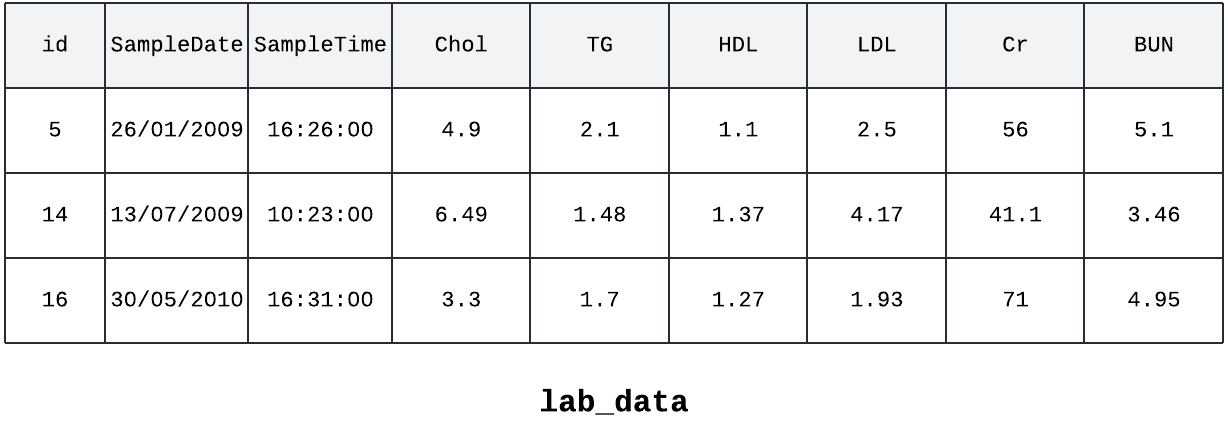
\includegraphics[width=0.8\linewidth]{images/03-Labs_DF} 

}

\caption{An illustration of a data frame containing patient haematology and biochemistry values.}\label{fig:labs-df}
\end{figure}

\textbf{Matrices}, \textbf{data frames}, and \textbf{tibbles} are stored in row, column notation, indexed from 1. So, \texttt{df{[}i,j{]}} will return the \texttt{ith} row and the \texttt{jth} column. For data structures with named columns, \texttt{\$} can be used to access the named variable.

Exploring dplyr's \texttt{select} function:

\begin{Shaded}
\begin{Highlighting}[]
\FunctionTok{library}\NormalTok{(dplyr)}
\NormalTok{lab\_data }\OtherTok{\textless{}{-}} \FunctionTok{data.frame}\NormalTok{(}\AttributeTok{id =} \FunctionTok{c}\NormalTok{(}\DecValTok{5}\NormalTok{, }\DecValTok{14}\NormalTok{, }\DecValTok{16}\NormalTok{), }
        \AttributeTok{SampleDate =} \FunctionTok{c}\NormalTok{(}\StringTok{"26{-}01{-}2009"}\NormalTok{, }\StringTok{"13{-}07{-}2009"}\NormalTok{, }\StringTok{"30{-}05{-}2010"}\NormalTok{), }
        \AttributeTok{SampleTime =} \FunctionTok{c}\NormalTok{(}\StringTok{"16:26:00"}\NormalTok{, }\StringTok{"10:23:00"}\NormalTok{, }\StringTok{"16:31:00"}\NormalTok{), }
        \AttributeTok{Chol =} \FunctionTok{c}\NormalTok{(}\FloatTok{4.9}\NormalTok{, }\FloatTok{6.49}\NormalTok{, }\FloatTok{3.3}\NormalTok{), }
        \AttributeTok{TG =} \FunctionTok{c}\NormalTok{(}\FloatTok{2.1}\NormalTok{, }\FloatTok{1.48}\NormalTok{, }\FloatTok{1.7}\NormalTok{), }
        \AttributeTok{HDL =} \FunctionTok{c}\NormalTok{(}\FloatTok{1.1}\NormalTok{, }\FloatTok{1.37}\NormalTok{, }\FloatTok{1.27}\NormalTok{), }
        \AttributeTok{LDL =} \FunctionTok{c}\NormalTok{(}\FloatTok{2.5}\NormalTok{, }\FloatTok{4.14}\NormalTok{, }\FloatTok{1.93}\NormalTok{),  }
        \AttributeTok{Cr =} \FunctionTok{c}\NormalTok{(}\FloatTok{56.0}\NormalTok{, }\FloatTok{41.1}\NormalTok{, }\DecValTok{71}\NormalTok{),}
        \AttributeTok{BUN =} \FunctionTok{c}\NormalTok{(}\FloatTok{5.1}\NormalTok{, }\FloatTok{3.46}\NormalTok{, }\FloatTok{4.95}\NormalTok{)) }

\CommentTok{\# Select a range of columns}
\NormalTok{lab\_data }\SpecialCharTok{\%\textgreater{}\%}\NormalTok{ dplyr}\SpecialCharTok{::}\FunctionTok{select}\NormalTok{(HDL}\SpecialCharTok{:}\NormalTok{Cr)}
\end{Highlighting}
\end{Shaded}

\begin{verbatim}
##    HDL  LDL   Cr
## 1 1.10 2.50 56.0
## 2 1.37 4.14 41.1
## 3 1.27 1.93 71.0
\end{verbatim}

\begin{Shaded}
\begin{Highlighting}[]
\CommentTok{\# Removing variables with "{-}"}
\NormalTok{lab\_data }\SpecialCharTok{\%\textgreater{}\%}\NormalTok{ dplyr}\SpecialCharTok{::}\FunctionTok{select}\NormalTok{(}\SpecialCharTok{{-}}\NormalTok{SampleTime)}
\end{Highlighting}
\end{Shaded}

\begin{verbatim}
##   id SampleDate Chol   TG  HDL  LDL   Cr  BUN
## 1  5 26-01-2009 4.90 2.10 1.10 2.50 56.0 5.10
## 2 14 13-07-2009 6.49 1.48 1.37 4.14 41.1 3.46
## 3 16 30-05-2010 3.30 1.70 1.27 1.93 71.0 4.95
\end{verbatim}

\subsection{Filtering}\label{sec:filtering}

In contrast to selecting, \textbf{filtering} deals with observations. Within \texttt{dplyr}, this is done with the \texttt{filter} function, where the filtering conditions are passed in as parameters.

Filtering examples using dplyr's \texttt{filter} function:

\begin{Shaded}
\begin{Highlighting}[]
\FunctionTok{library}\NormalTok{(dplyr)}

\CommentTok{\# Select all observations where TG \textgreater{} 1.5}
\NormalTok{lab\_data }\SpecialCharTok{\%\textgreater{}\%}\NormalTok{ dplyr}\SpecialCharTok{::}\FunctionTok{filter}\NormalTok{(TG }\SpecialCharTok{\textgreater{}} \FloatTok{1.5}\NormalTok{)}
\end{Highlighting}
\end{Shaded}

\begin{verbatim}
##   id SampleDate SampleTime Chol  TG  HDL  LDL Cr  BUN
## 1  5 26-01-2009   16:26:00  4.9 2.1 1.10 2.50 56 5.10
## 2 16 30-05-2010   16:31:00  3.3 1.7 1.27 1.93 71 4.95
\end{verbatim}

\begin{Shaded}
\begin{Highlighting}[]
\CommentTok{\# Or combine to filter on multiple conditions}
\NormalTok{lab\_data }\SpecialCharTok{\%\textgreater{}\%}\NormalTok{ dplyr}\SpecialCharTok{::}\FunctionTok{filter}\NormalTok{((TG }\SpecialCharTok{\textgreater{}} \FloatTok{1.5}\NormalTok{) }\SpecialCharTok{\&}\NormalTok{ (HDL }\SpecialCharTok{\textless{}} \FloatTok{1.2}\NormalTok{))}
\end{Highlighting}
\end{Shaded}

\begin{verbatim}
##   id SampleDate SampleTime Chol  TG HDL LDL Cr BUN
## 1  5 26-01-2009   16:26:00  4.9 2.1 1.1 2.5 56 5.1
\end{verbatim}

\subsection{If/Else}\label{sec:ifElse}

Within R, and many other coding languages, an \textbf{if statement} is a block of code that will only execute if the condition inside the parentheses is \texttt{TRUE}. Often, there will be an associated \textbf{else} code block that will execute only if the if statement was false.

\subsubsection{Element-Wise Comparisons}\label{sec:if_else}

\textbf{Element-wise} comparisons work across vectors, touching each element within the vector. The base R version of \texttt{ifelse} takes the format of \texttt{base::ifelse(test,\ yes,\ no)}.

Examples of using \texttt{ifelse}:

\begin{Shaded}
\begin{Highlighting}[]
\NormalTok{a }\OtherTok{\textless{}{-}} \FunctionTok{c}\NormalTok{(}\DecValTok{1}\NormalTok{, }\DecValTok{2}\NormalTok{, }\DecValTok{3}\NormalTok{)}

\CommentTok{\# Example 1: Replace even numbers with TRUE and odds with FALSE}
\NormalTok{base}\SpecialCharTok{::}\FunctionTok{ifelse}\NormalTok{(a }\SpecialCharTok{\%\%} \DecValTok{2} \SpecialCharTok{==} \DecValTok{0}\NormalTok{, }\ConstantTok{TRUE}\NormalTok{, }\ConstantTok{FALSE}\NormalTok{)}
\end{Highlighting}
\end{Shaded}

\begin{verbatim}
## [1] FALSE  TRUE FALSE
\end{verbatim}

\begin{Shaded}
\begin{Highlighting}[]
\CommentTok{\#Example 3: NA values}
\NormalTok{a }\OtherTok{\textless{}{-}} \FunctionTok{c}\NormalTok{(}\DecValTok{1}\NormalTok{, }\DecValTok{2}\NormalTok{, }\ConstantTok{NA}\NormalTok{)}
\NormalTok{base}\SpecialCharTok{::}\FunctionTok{ifelse}\NormalTok{(a }\SpecialCharTok{\%\%} \DecValTok{2} \SpecialCharTok{==} \DecValTok{0}\NormalTok{, }\ConstantTok{TRUE}\NormalTok{, }\ConstantTok{FALSE}\NormalTok{)}
\end{Highlighting}
\end{Shaded}

\begin{verbatim}
## [1] FALSE  TRUE    NA
\end{verbatim}

In the tidyverse world, this type of functionality has been implemented using the \texttt{if\_else} function within the \texttt{dplyr} package. It has a slightly more explicit formulation about how missing values are handled.

Example using dplyr's \texttt{if\_else}:

\begin{Shaded}
\begin{Highlighting}[]
\NormalTok{a }\OtherTok{\textless{}{-}} \FunctionTok{c}\NormalTok{(}\DecValTok{1}\NormalTok{, }\DecValTok{2}\NormalTok{, }\ConstantTok{NA}\NormalTok{)}
\NormalTok{(dplyr}\SpecialCharTok{::}\FunctionTok{if\_else}\NormalTok{(a }\SpecialCharTok{\%\%} \DecValTok{2} \SpecialCharTok{==} \DecValTok{0}\NormalTok{, }\ConstantTok{TRUE}\NormalTok{, }\ConstantTok{FALSE}\NormalTok{, }\AttributeTok{missing =} \ConstantTok{NULL}\NormalTok{))}
\end{Highlighting}
\end{Shaded}

\begin{verbatim}
## [1] FALSE  TRUE    NA
\end{verbatim}

\begin{Shaded}
\begin{Highlighting}[]
\CommentTok{\# Instead, change all missing values to FALSE}
\NormalTok{(dplyr}\SpecialCharTok{::}\FunctionTok{if\_else}\NormalTok{(a }\SpecialCharTok{\%\%} \DecValTok{2} \SpecialCharTok{==} \DecValTok{0}\NormalTok{, }\ConstantTok{TRUE}\NormalTok{, }\ConstantTok{FALSE}\NormalTok{, }\AttributeTok{missing =} \ConstantTok{FALSE}\NormalTok{))}
\end{Highlighting}
\end{Shaded}

\begin{verbatim}
## [1] FALSE  TRUE FALSE
\end{verbatim}

\subsubsection{Logic Flow}\label{logic-flow}

\begin{figure}

{\centering 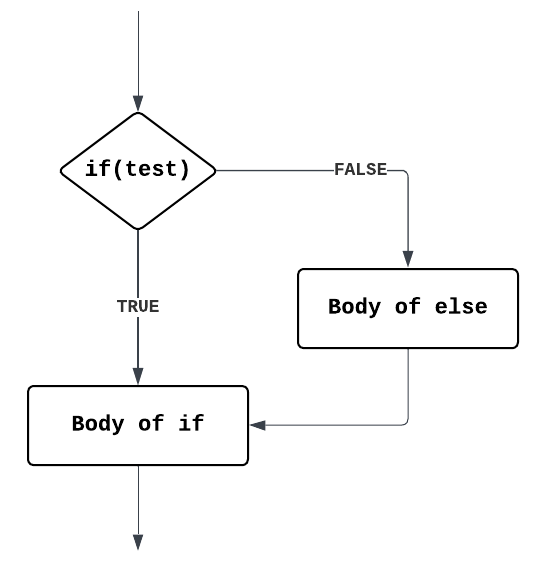
\includegraphics[width=0.5\linewidth]{images/03-ifElse} 

}

\caption{A flowchart of how an if/else statement is executed}\label{fig:if-else-flowchart}
\end{figure}

\textbf{Logic flow} if/else statements are often used to set an internal parameter within a function based on a passed parameter. The \texttt{if} function tests to see if the provided conditional evaluates to \texttt{TRUE}. If it does, the code within the body of the if statement defined by \texttt{\{\}} will be executed in sequence; otherwise, the code within the \texttt{else} block, if it exists, will be executed.

\subsection{Multiple Comparisons}\label{sec:CaseWhen}

If/else is a great option when there is one comparison and two possible options. When there are multiple exclusive comparisons to be made, the \texttt{case\_when} function within the \texttt{dplyr} package exists for when \texttt{if\_else} is too simple.

Multiple comparisons within one \texttt{case\_when} with an informative default:

\begin{Shaded}
\begin{Highlighting}[]
\NormalTok{demog }\OtherTok{\textless{}{-}}\NormalTok{ utils}\SpecialCharTok{::}\FunctionTok{read.csv}\NormalTok{(}\StringTok{"data/03{-}diabetic\_demog.csv"}\NormalTok{, }\AttributeTok{head =} \ConstantTok{TRUE}\NormalTok{)}
    
\CommentTok{\# Now using case\_when()}
\NormalTok{demog }\OtherTok{\textless{}{-}}\NormalTok{ demog }\SpecialCharTok{\%\textgreater{}\%}\NormalTok{ dplyr}\SpecialCharTok{::}\FunctionTok{mutate}\NormalTok{(}
    \AttributeTok{bmi\_obesity\_level =}\NormalTok{ dplyr}\SpecialCharTok{::}\FunctionTok{case\_when}\NormalTok{(}
                            \FunctionTok{is.na}\NormalTok{(BMI) }\SpecialCharTok{\textasciitilde{}} \ConstantTok{NA}\NormalTok{, }\CommentTok{\#added check for NA values}
\NormalTok{                            BMI }\SpecialCharTok{\textless{}} \FloatTok{18.5} \SpecialCharTok{\textasciitilde{}} \StringTok{"underweight"}\NormalTok{, }
\NormalTok{                            BMI }\SpecialCharTok{\textless{}} \DecValTok{25} \SpecialCharTok{\textasciitilde{}} \StringTok{"healthy weight"}\NormalTok{,}
\NormalTok{                            BMI }\SpecialCharTok{\textless{}} \DecValTok{30} \SpecialCharTok{\textasciitilde{}} \StringTok{"overweight"}\NormalTok{, }
\NormalTok{                            BMI }\SpecialCharTok{\textless{}} \DecValTok{40} \SpecialCharTok{\textasciitilde{}} \StringTok{"obese"}\NormalTok{,}
\NormalTok{                            BMI }\SpecialCharTok{\textgreater{}=} \DecValTok{40} \SpecialCharTok{\textasciitilde{}} \StringTok{"morbidly obese"}\NormalTok{, }\CommentTok{\# added case}
                            \AttributeTok{.default =} \StringTok{"logic error"} \CommentTok{\#informative logic check}
\NormalTok{                        ) }\CommentTok{\#close case\_when()}
\NormalTok{                    ) }\CommentTok{\#close mutate()}
                    
\CommentTok{\# Turn into a factor}
\NormalTok{demog}\SpecialCharTok{$}\NormalTok{bmi\_obesity\_level }\OtherTok{\textless{}{-}}\NormalTok{ base}\SpecialCharTok{::}\FunctionTok{as.factor}\NormalTok{(demog}\SpecialCharTok{$}\NormalTok{bmi\_obesity\_level)}

\CommentTok{\# Get a summary and look for any error values}
\NormalTok{base}\SpecialCharTok{::}\FunctionTok{summary}\NormalTok{(demog}\SpecialCharTok{$}\NormalTok{bmi\_obesity\_level)}
\end{Highlighting}
\end{Shaded}

\begin{verbatim}
## healthy weight morbidly obese          obese     overweight    underweight 
##             19             23             96             53              6
\end{verbatim}

\subsection{Loops}\label{sec:loops}

R uses loops to repeat tasks, which means that the code can be written and tested once but repeated numerous times. There are two main classifications of loops within R, the \textbf{\texttt{for\ loop}} and the \textbf{\texttt{while\ loop}}.

\subsubsection{For loops}\label{sec:forLoops}

The \textbf{\texttt{for\ loop}} is best used when a chunk of code should be run for a known number of times.

A simple implementation:

\begin{Shaded}
\begin{Highlighting}[]
\ControlFlowTok{for}\NormalTok{ (i }\ControlFlowTok{in} \DecValTok{1}\SpecialCharTok{:}\DecValTok{4}\NormalTok{)\{}
\NormalTok{    base}\SpecialCharTok{::}\FunctionTok{print}\NormalTok{(i)}
\NormalTok{\}}
\end{Highlighting}
\end{Shaded}

\begin{verbatim}
## [1] 1
## [1] 2
## [1] 3
## [1] 4
\end{verbatim}

\subsubsection{While loops}\label{sec:whileLoops}

\texttt{For\ loops} execute a chunk of code for a set and pre-defined number of times, while \textbf{\texttt{while\ loops}} execute as long as the test condition iterates to \texttt{TRUE}, i.e., the exact number of iterations is unknown.

A simple while loop controlled by a counting functionality:

\begin{Shaded}
\begin{Highlighting}[]
\CommentTok{\# define the incremental value}
\NormalTok{n }\OtherTok{=} \DecValTok{1}
\ControlFlowTok{while}\NormalTok{(n }\SpecialCharTok{\textless{}} \DecValTok{3}\NormalTok{)\{}
\NormalTok{    base}\SpecialCharTok{::}\FunctionTok{print}\NormalTok{(n)}
    \CommentTok{\# Increment n}
\NormalTok{    n }\OtherTok{=}\NormalTok{ n }\SpecialCharTok{+} \DecValTok{1}
\NormalTok{\}}
\end{Highlighting}
\end{Shaded}

\begin{verbatim}
## [1] 1
## [1] 2
\end{verbatim}

\section{Merging datasets}\label{sec:merging}

Very rarely will datasets be presented as `analysis-ready'. Data are often provided in separate tables and need to be combined into one, final, `analysis-ready' table. This is done by \textbf{merging} tables using a variety of \textbf{\texttt{joins}}.

\subsection{The Mechanics}\label{the-mechanics}

Joins work by connecting tables through a pair of \textbf{keys}, or a specified variable within each table that identifies an observation within a table. There are two types of keys: \textbf{\texttt{primary}} and \textbf{\texttt{foreign\ keys}}.

\begin{figure}

{\centering 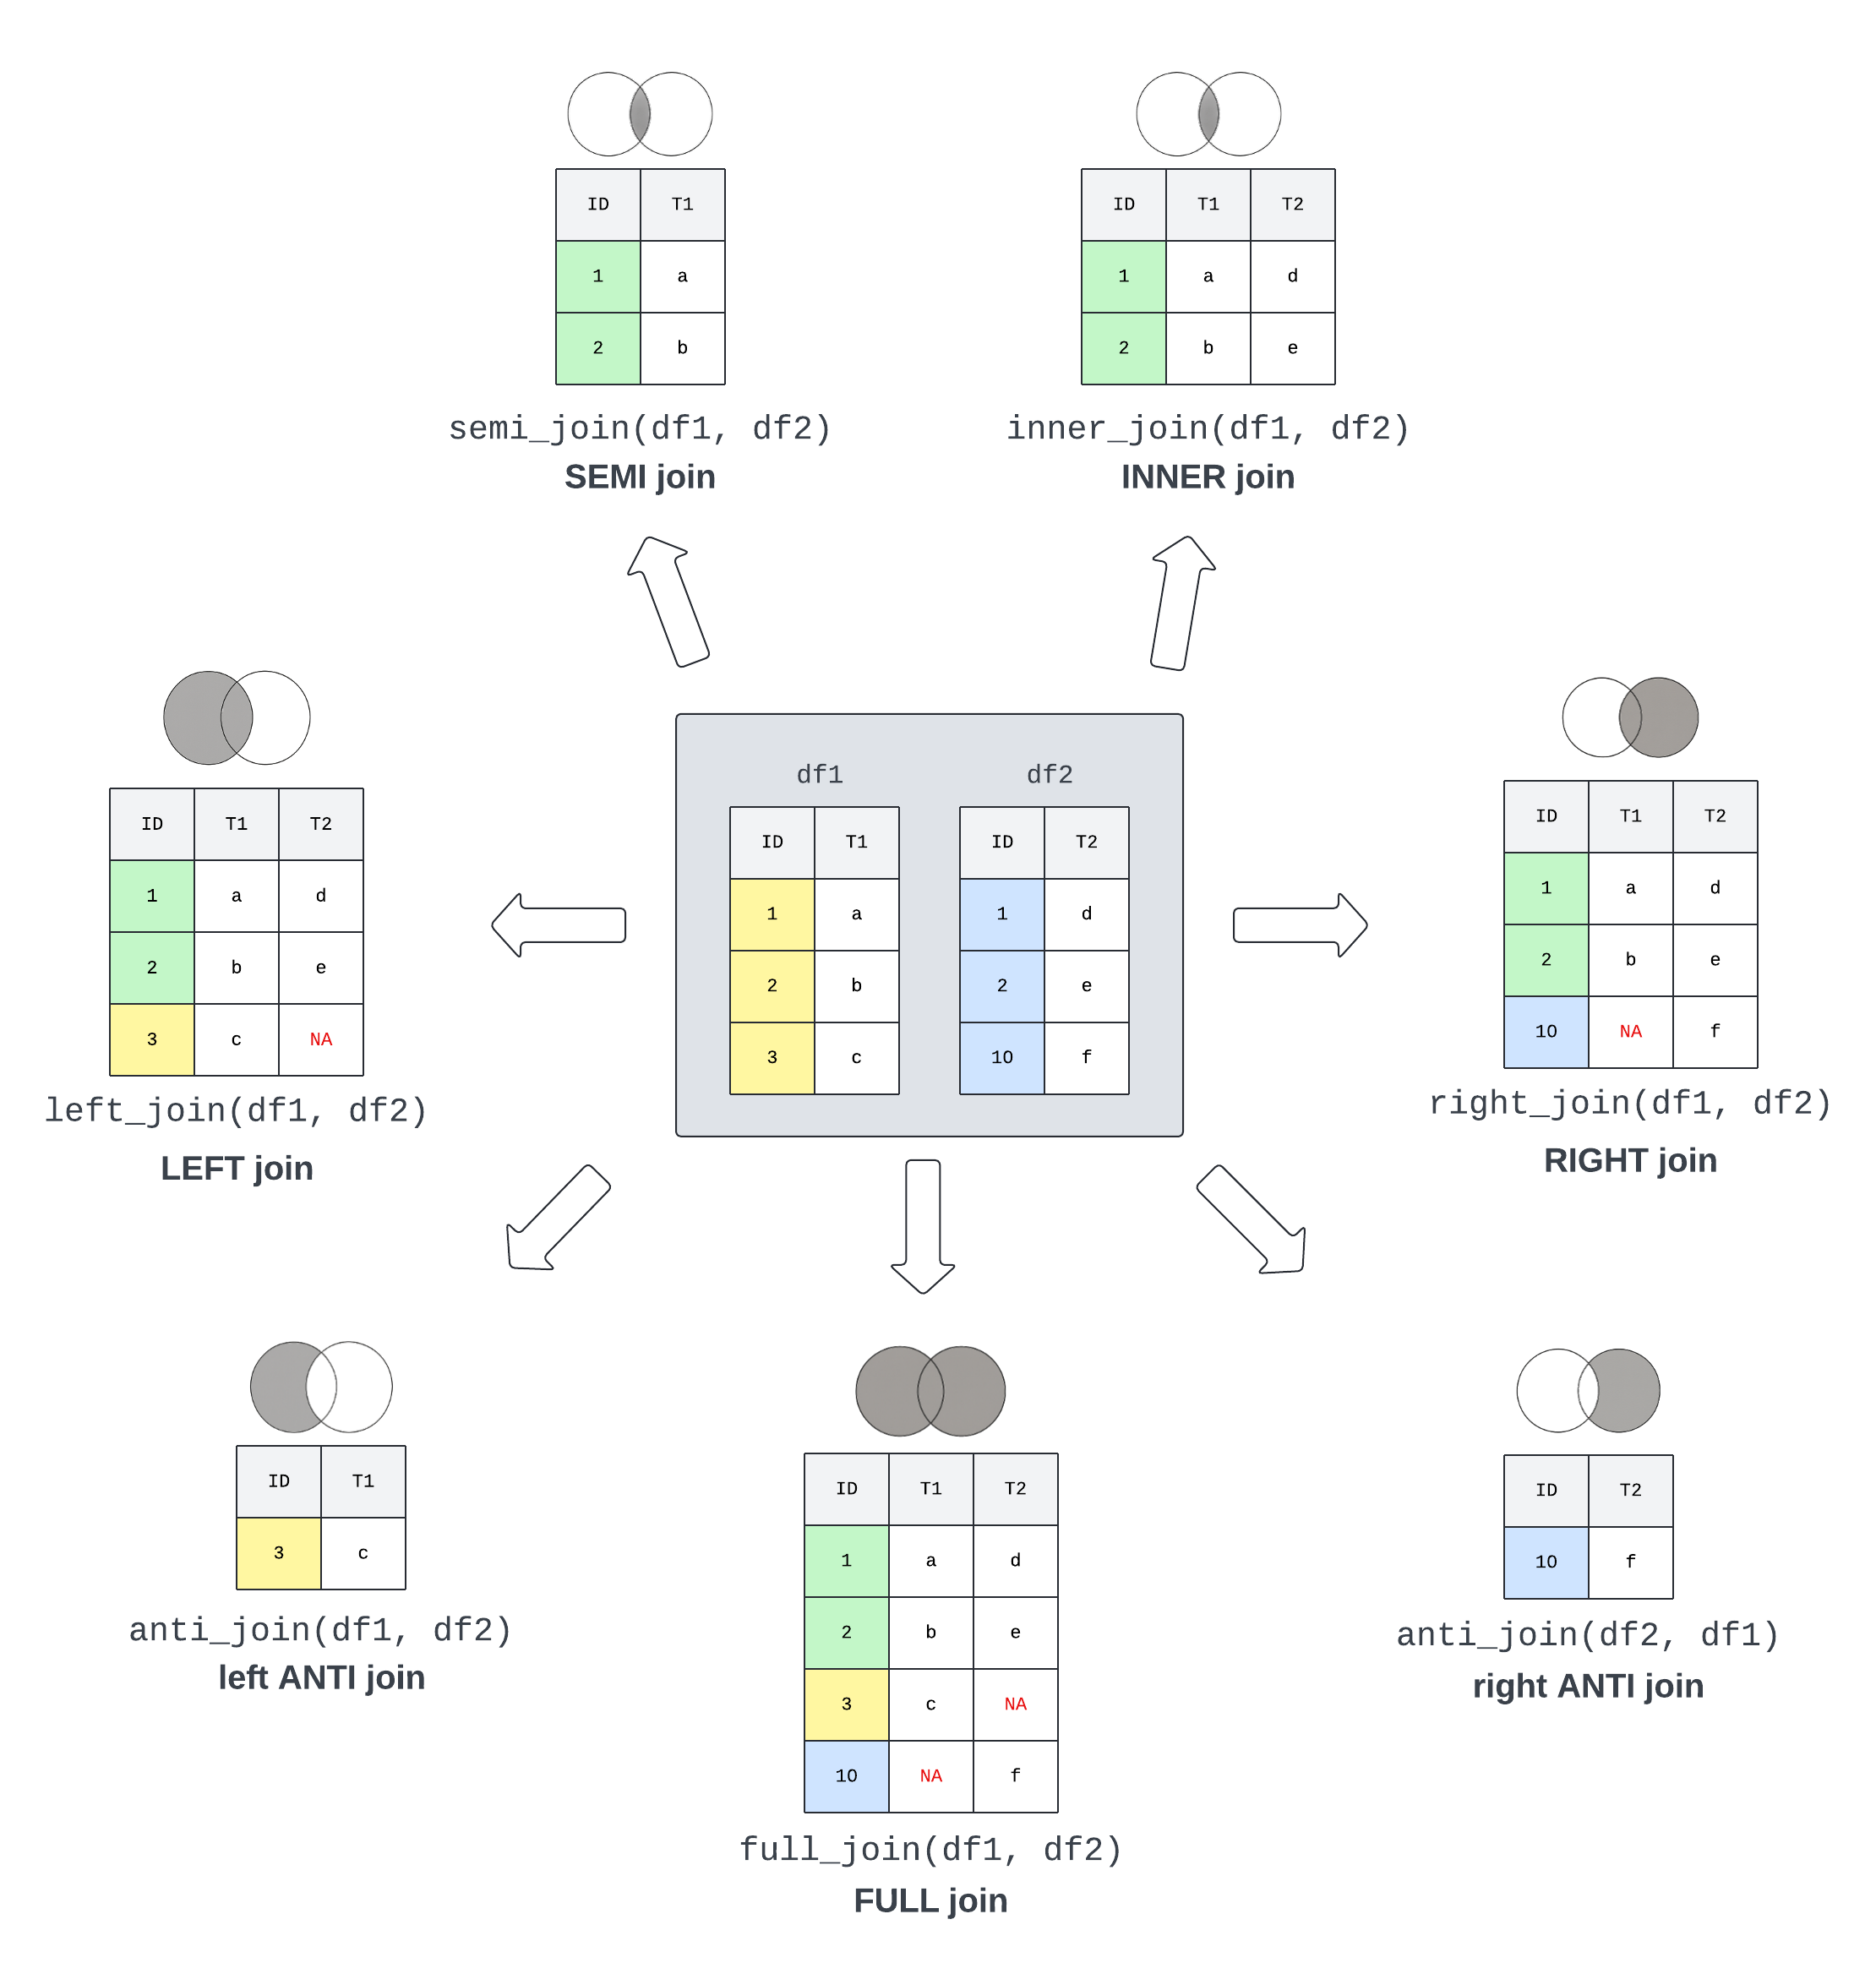
\includegraphics[width=1\linewidth]{images/03-joins} 

}

\caption{An illustration of the most common joins used to combine information from two data frames used within dplyr, including code fragments. The Venn diagrams illustrate how the two data frames are integrated, while the tables illustrate the resulting data frames.}\label{fig:joins-diagram}
\end{figure}

\subsubsection{Checking Primary Keys}\label{sec:checkingPrimaryKeys}

There are two things to worry about regarding primary keys: (1) they are unique, and (2) they are not missing.

Check to see if the primary keys are unique:

\begin{Shaded}
\begin{Highlighting}[]
\CommentTok{\# Demographics}
\NormalTok{demog }\OtherTok{\textless{}{-}}\NormalTok{ utils}\SpecialCharTok{::}\FunctionTok{read.csv}\NormalTok{(}\StringTok{"data/03{-}diabetic\_demog.csv"}\NormalTok{)}

\DocumentationTok{\#\# count the number of times the primary key is seen}
\NormalTok{demog }\SpecialCharTok{\%\textgreater{}\%}\NormalTok{ dplyr}\SpecialCharTok{::}\FunctionTok{count}\NormalTok{(id) }\SpecialCharTok{\%\textgreater{}\%} 
\DocumentationTok{\#\# filter for counts more than 1}
\NormalTok{    dplyr}\SpecialCharTok{::}\FunctionTok{filter}\NormalTok{(n }\SpecialCharTok{\textgreater{}} \DecValTok{1}\NormalTok{)}
\end{Highlighting}
\end{Shaded}

\begin{verbatim}
## [1] id n 
## <0 rows> (or 0-length row.names)
\end{verbatim}

\begin{Shaded}
\begin{Highlighting}[]
\CommentTok{\# Lab data}
\NormalTok{lab\_data }\OtherTok{\textless{}{-}}\NormalTok{ utils}\SpecialCharTok{::}\FunctionTok{read.csv}\NormalTok{(}\StringTok{"data/03{-}diabetic\_labs\_final\_with\_missing.csv"}\NormalTok{)}

\DocumentationTok{\#\# count the number of times the primary key is seen}
\NormalTok{utils}\SpecialCharTok{::}\FunctionTok{head}\NormalTok{(lab\_data }\SpecialCharTok{\%\textgreater{}\%}\NormalTok{ dplyr}\SpecialCharTok{::}\FunctionTok{count}\NormalTok{(id) }\SpecialCharTok{\%\textgreater{}\%} 
\DocumentationTok{\#\# filter for counts more than 1}
\NormalTok{    dplyr}\SpecialCharTok{::}\FunctionTok{filter}\NormalTok{(n }\SpecialCharTok{\textgreater{}} \DecValTok{1}\NormalTok{), }\AttributeTok{n =} \DecValTok{4}\DataTypeTok{L}\NormalTok{)}
\end{Highlighting}
\end{Shaded}

\begin{verbatim}
##   id n
## 1  5 3
## 2 14 3
## 3 16 3
## 4 25 2
\end{verbatim}

The zero returned rows indicate that diabeticDemog has no repeated keys. In contrast, the numerous rows from diabeticLabs indicate that \texttt{id} is not enough to identify a row uniquely, so joining these two tables using only the \texttt{id} column produces a \textbf{many-to-one} join.

\subsubsection{Introduction to Joining}\label{sec:IntroToJoining}

There are two ways to join two tables. The first is to pass the table using a pipe to pass one table (the \textbf{left} table) to one of the join functions, where the second table is passed in as the first argument (this table is referred to as the \textbf{right} table).

Example of an inner join:

\begin{Shaded}
\begin{Highlighting}[]
\NormalTok{demog }\OtherTok{\textless{}{-}}\NormalTok{ utils}\SpecialCharTok{::}\FunctionTok{read.csv}\NormalTok{(}\StringTok{"data/03{-}diabetic\_demog.csv"}\NormalTok{)}
\NormalTok{lab\_data }\OtherTok{\textless{}{-}}\NormalTok{ utils}\SpecialCharTok{::}\FunctionTok{read.csv}\NormalTok{(}\StringTok{"data/03{-}diabetic\_labs\_final\_with\_missing.csv"}\NormalTok{)}

\CommentTok{\# method 1}
\NormalTok{joined1 }\OtherTok{\textless{}{-}}\NormalTok{ demog }\SpecialCharTok{\%\textgreater{}\%}\NormalTok{ dplyr}\SpecialCharTok{::}\FunctionTok{inner\_join}\NormalTok{(lab\_data, }\AttributeTok{by=}\StringTok{"id"}\NormalTok{)}
\NormalTok{utils}\SpecialCharTok{::}\FunctionTok{head}\NormalTok{(joined1, }\AttributeTok{n =} \DecValTok{3}\DataTypeTok{L}\NormalTok{)}
\end{Highlighting}
\end{Shaded}

\begin{verbatim}
##   id age Gender BMI SIMD SampleDate SampleTime Chol   TG      HDL      LDL   Cr
## 1  5  28      M  26    4 26/01/2009   16:26:00 4.90 2.10 1.100000 2.500000 56.0
## 2  5  28      M  26    4 19/10/2012   10:22:00 3.60 5.10 0.900000 2.500000 63.0
## 3  5  28      M  26    4 19/10/2012   09:31:00 4.85 1.63 4.860753 4.860753 96.7
##    BUN
## 1 5.10
## 2 5.00
## 3 5.24
\end{verbatim}

\begin{Shaded}
\begin{Highlighting}[]
\CommentTok{\# method 2}
\NormalTok{joined2 }\OtherTok{\textless{}{-}}\NormalTok{ dplyr}\SpecialCharTok{::}\FunctionTok{inner\_join}\NormalTok{(demog, lab\_data, }\AttributeTok{by =} \StringTok{"id"}\NormalTok{)}
\NormalTok{utils}\SpecialCharTok{::}\FunctionTok{head}\NormalTok{(joined2, }\AttributeTok{n =} \DecValTok{3}\DataTypeTok{L}\NormalTok{)}
\end{Highlighting}
\end{Shaded}

\begin{verbatim}
##   id age Gender BMI SIMD SampleDate SampleTime Chol   TG      HDL      LDL   Cr
## 1  5  28      M  26    4 26/01/2009   16:26:00 4.90 2.10 1.100000 2.500000 56.0
## 2  5  28      M  26    4 19/10/2012   10:22:00 3.60 5.10 0.900000 2.500000 63.0
## 3  5  28      M  26    4 19/10/2012   09:31:00 4.85 1.63 4.860753 4.860753 96.7
##    BUN
## 1 5.10
## 2 5.00
## 3 5.24
\end{verbatim}

\section{Cautionary Tale}\label{sec:cautionaryTale}

\subsection{Check for Uniqueness}\label{sec:checkForUniqueness}

Often, in the course of health data science, statistical analysis plans may request the first or lowest value. In the case of the first or last test, what happens if there is more than one test on the same day? For this reason, add additional columns to sort by so that ties are broken and unique values are therefore selected.

Now add an additional value to break the ties

\begin{Shaded}
\begin{Highlighting}[]
\FunctionTok{library}\NormalTok{(tidyverse)}
\FunctionTok{library}\NormalTok{(hms)}
\NormalTok{lab\_data }\OtherTok{\textless{}{-}}\NormalTok{ utils}\SpecialCharTok{::}\FunctionTok{read.csv}\NormalTok{(}\StringTok{"data/03{-}diabetic\_labs\_final\_with\_missing.csv"}\NormalTok{)}

\CommentTok{\# Convert dates and times}
\NormalTok{lab\_data}\SpecialCharTok{$}\NormalTok{SampleDate }\OtherTok{\textless{}{-}}\NormalTok{ lubridate}\SpecialCharTok{::}\FunctionTok{as\_date}\NormalTok{(}
\NormalTok{        lab\_data}\SpecialCharTok{$}\NormalTok{SampleDate, }\AttributeTok{format =} \StringTok{"\%d/\%m/\%Y"}\NormalTok{)}
\NormalTok{lab\_data}\SpecialCharTok{$}\NormalTok{SampleTime }\OtherTok{\textless{}{-}}\NormalTok{ hms}\SpecialCharTok{::}\FunctionTok{as\_hms}\NormalTok{(lubridate}\SpecialCharTok{::}\FunctionTok{as\_datetime}\NormalTok{(}
\NormalTok{  lab\_data}\SpecialCharTok{$}\NormalTok{SampleTime, }\AttributeTok{format =} \StringTok{"\%H:\%M:\%S"}\NormalTok{))}

\CommentTok{\# collect the last test value and print the first 10 rows}
\NormalTok{utils}\SpecialCharTok{::}\FunctionTok{head}\NormalTok{(lab\_data }\SpecialCharTok{\%\textgreater{}\%} 
    \CommentTok{\# sort by id, date, and time in descending order}
\NormalTok{    dplyr}\SpecialCharTok{::}\FunctionTok{arrange}\NormalTok{(id, dplyr}\SpecialCharTok{::}\FunctionTok{desc}\NormalTok{(SampleDate), dplyr}\SpecialCharTok{::}\FunctionTok{desc}\NormalTok{(SampleTime)) }\SpecialCharTok{\%\textgreater{}\%} 
    \CommentTok{\# group by id and SampleDate to break ties}
\NormalTok{    dplyr}\SpecialCharTok{::}\FunctionTok{group\_by}\NormalTok{(id, SampleDate) }\SpecialCharTok{\%\textgreater{}\%} 
    \CommentTok{\# add a rank to see ties }
\NormalTok{    dplyr}\SpecialCharTok{::}\FunctionTok{mutate}\NormalTok{(}\AttributeTok{rank =}\NormalTok{ dplyr}\SpecialCharTok{::}\FunctionTok{min\_rank}\NormalTok{(dplyr}\SpecialCharTok{::}\FunctionTok{desc}\NormalTok{(SampleTime))),}
    \AttributeTok{n =} \DecValTok{10}\DataTypeTok{L}\NormalTok{)}
\end{Highlighting}
\end{Shaded}

\begin{verbatim}
## # A tibble: 10 x 10
## # Groups:   id, SampleDate [9]
##       id SampleDate SampleTime  Chol    TG   HDL   LDL    Cr   BUN  rank
##    <int> <date>     <time>     <dbl> <dbl> <dbl> <dbl> <dbl> <dbl> <int>
##  1     5 2012-10-19 10:22       3.6   5.1   0.9   2.5   63    5        1
##  2     5 2012-10-19 09:31       4.85  1.63  4.86  4.86  96.7  5.24     2
##  3     5 2009-01-26 16:26       4.9   2.1   1.1   2.5   56    5.1      1
##  4    14 2011-02-22 13:11       4.8   1     1.72  2.57  73    4.67     1
##  5    14 2010-10-07 11:05      NA     0.92  4.86  4.86  60    4.72     1
##  6    14 2009-07-13 10:23       6.49  1.48  1.37  4.17  41.1  3.46     1
##  7    16 2012-06-24 12:34       5.4   1.6   1.6   3.1   NA    4.1      1
##  8    16 2012-02-17 10:43       4.31  0.84  4.86  4.86  66    7.23     1
##  9    16 2010-05-30 16:31       3.3   1.7   1.27  1.93  71    4.95     1
## 10    25 2011-10-16 10:41       4.6   1.2   1.3   2.8   49    3.2      1
\end{verbatim}

\subsection{Cartesian product joins}\label{sec:CartesianProduct}

Below is a toy example to illustrate how quickly \textbf{many-to-many} joins can produce undesired results due to the Cartesian product.

Cartesian product due to many-to-many matches:

\begin{Shaded}
\begin{Highlighting}[]
\NormalTok{df1 }\OtherTok{\textless{}{-}}\NormalTok{ dplyr}\SpecialCharTok{::}\FunctionTok{tibble}\NormalTok{(}
        \AttributeTok{id =} \FunctionTok{c}\NormalTok{(}\DecValTok{1}\NormalTok{, }\DecValTok{1}\NormalTok{, }\DecValTok{2}\NormalTok{), }
        \AttributeTok{value1 =} \FunctionTok{c}\NormalTok{(}\StringTok{"a"}\NormalTok{, }\StringTok{"b"}\NormalTok{, }\StringTok{"c"}\NormalTok{)}
\NormalTok{        )}
\NormalTok{df2 }\OtherTok{\textless{}{-}}\NormalTok{ dplyr}\SpecialCharTok{::}\FunctionTok{tibble}\NormalTok{(}
        \AttributeTok{id =} \FunctionTok{c}\NormalTok{(}\DecValTok{1}\NormalTok{, }\DecValTok{2}\NormalTok{, }\DecValTok{2}\NormalTok{),}
        \AttributeTok{value2 =} \FunctionTok{c}\NormalTok{(}\StringTok{"x"}\NormalTok{, }\StringTok{"y"}\NormalTok{, }\StringTok{"z"}\NormalTok{)}
\NormalTok{        )}

\CommentTok{\# Depending on dplyr version, this may throw a warning}
\NormalTok{df1 }\SpecialCharTok{\%\textgreater{}\%}\NormalTok{ dplyr}\SpecialCharTok{::}\FunctionTok{inner\_join}\NormalTok{(df2, }\AttributeTok{by =} \StringTok{"id"}\NormalTok{)}
\end{Highlighting}
\end{Shaded}

\begin{verbatim}
## Warning in dplyr::inner_join(., df2, by = "id"): Detected an unexpected many-to-many relationship between `x` and `y`.
## i Row 3 of `x` matches multiple rows in `y`.
## i Row 1 of `y` matches multiple rows in `x`.
## i If a many-to-many relationship is expected, set `relationship =
##   "many-to-many"` to silence this warning.
\end{verbatim}

\begin{verbatim}
## # A tibble: 4 x 3
##      id value1 value2
##   <dbl> <chr>  <chr> 
## 1     1 a      x     
## 2     1 b      x     
## 3     2 c      y     
## 4     2 c      z
\end{verbatim}

\chapter{Data Visualisation}\label{ch-4}

\begin{center}
\includegraphics[width=0.5\linewidth]{images/04-ggplot_Logo} \end{center}

Before starting this chapter, make sure that you have the following R packages installed and loaded.

\begin{Shaded}
\begin{Highlighting}[]
\CommentTok{\#Install packages}
\NormalTok{utils}\SpecialCharTok{::}\FunctionTok{install.packages}\NormalTok{(}\StringTok{"ggplot2"}\NormalTok{) }\CommentTok{\#also installed via tidyverse}
\NormalTok{utils}\SpecialCharTok{::}\FunctionTok{install.packages}\NormalTok{(}\StringTok{"patchwork"}\NormalTok{)}
\NormalTok{utils}\SpecialCharTok{::}\FunctionTok{install.packages}\NormalTok{(}\StringTok{"dplyr"}\NormalTok{) }\CommentTok{\#also installed via tidyverse}
\NormalTok{utils}\SpecialCharTok{::}\FunctionTok{install.packages}\NormalTok{(}\StringTok{"viridis"}\NormalTok{)}
\end{Highlighting}
\end{Shaded}

Remember you only need to install package once in a computer. And after they're installed you can load them into the current R session:

\begin{Shaded}
\begin{Highlighting}[]
\CommentTok{\#Load packages}
\NormalTok{base}\SpecialCharTok{::}\FunctionTok{library}\NormalTok{(ggplot2)}
\NormalTok{base}\SpecialCharTok{::}\FunctionTok{library}\NormalTok{(patchwork)}
\NormalTok{base}\SpecialCharTok{::}\FunctionTok{library}\NormalTok{(dplyr)}
\NormalTok{base}\SpecialCharTok{::}\FunctionTok{library}\NormalTok{(viridis)}
\end{Highlighting}
\end{Shaded}

\begin{verbatim}
## Loading required package: viridisLite
\end{verbatim}

\begin{Shaded}
\begin{Highlighting}[]
\FunctionTok{rm}\NormalTok{(}\AttributeTok{list=}\FunctionTok{ls}\NormalTok{()); }\FunctionTok{gc}\NormalTok{()}
\end{Highlighting}
\end{Shaded}

\begin{verbatim}
##           used  (Mb) gc trigger  (Mb) max used  (Mb)
## Ncells 2418252 129.2    4157530 222.1  4157530 222.1
## Vcells 4311053  32.9   10146329  77.5  8388608  64.0
\end{verbatim}

\section{Basic plotting}\label{basic-plotting}

There are two main methods for creating plots in R. We will be using the package ggplot2, which uses the grammar of graphics (a framework for building plots from components such as data, aesthetics, and facets), and we will be using some built-in data sets to start plotting.

The data set we are using for this walk-through is called iris and documents the sepal and petal length and width of three different species of iris. It is one of a number of built-in datasets that come with every installation of R, and it looks like this:

\begin{Shaded}
\begin{Highlighting}[]
\NormalTok{utils}\SpecialCharTok{::}\FunctionTok{data}\NormalTok{(iris)  }
\NormalTok{utils}\SpecialCharTok{::}\FunctionTok{head}\NormalTok{(iris) }
\end{Highlighting}
\end{Shaded}

\begin{verbatim}
##   Sepal.Length Sepal.Width Petal.Length Petal.Width Species
## 1          5.1         3.5          1.4         0.2  setosa
## 2          4.9         3.0          1.4         0.2  setosa
## 3          4.7         3.2          1.3         0.2  setosa
## 4          4.6         3.1          1.5         0.2  setosa
## 5          5.0         3.6          1.4         0.2  setosa
## 6          5.4         3.9          1.7         0.4  setosa
\end{verbatim}

\textbf{Explore the data:}
1. What is the range of Sepal.Length?
2. What is the mean of Sepal.Width?
3. What are the names of the three different iris species?

There are many options for how we can plot parts of this data frame, but our first example will be a scatter plot comparing sepal length and sepal width. Each plot should be considered as being made up of a number of layers, so we will build the plot layer by layer.

\subsection{Data layer}\label{data-layer}

The first line of any plot using ggplot2 starts with a call to ggplot. This can either be stand-alone as ggplot or we can define some of the key inputs for the plot. With a few exceptions, it is useful to include the dataset within this call to ggplot (either \textbf{\texttt{ggplot(dataname)}} or \textbf{\texttt{ggplot(data\ =\ dataname)}}). Beyond that, we can also specify some of the aesthetics of the graph - for example, what data is plotted on the x and y axes, and whether there is a grouping that we want to distinguish within the plot by colour, shape, or shading.

We are using the iris dataset and will plot the sepal length against the sepal width in this example, so our code line to set up the base canvas for the plot uses \textbf{\texttt{data\ =\ iris}} and \textbf{\texttt{aes(x\ =\ Sepal.Length,\ y\ =\ Sepal.Width)}}. Both versions of the code below produce the same plot:

Code example 1:

\begin{Shaded}
\begin{Highlighting}[]
\NormalTok{ggplot2}\SpecialCharTok{::}\FunctionTok{ggplot}\NormalTok{(iris, }\FunctionTok{aes}\NormalTok{(}\AttributeTok{x =}\NormalTok{ Sepal.Length, }\AttributeTok{y =}\NormalTok{ Sepal.Width))}
\end{Highlighting}
\end{Shaded}

\pandocbounded{\includegraphics[keepaspectratio]{_main_files/figure-latex/unnamed-chunk-97-1.pdf}}

Code example 2:

\begin{Shaded}
\begin{Highlighting}[]
\NormalTok{ggplot2}\SpecialCharTok{::}\FunctionTok{ggplot}\NormalTok{(}\AttributeTok{data =}\NormalTok{ iris, }\FunctionTok{aes}\NormalTok{(}\AttributeTok{x =}\NormalTok{ Sepal.Length, }\AttributeTok{y =}\NormalTok{ Sepal.Width))}
\end{Highlighting}
\end{Shaded}

\textbf{Try it yourself:}
1. What happens if you remove one of the x or y values in the \textbf{\texttt{aes}} argument?
2. What happens if you remove the \textbf{\texttt{aes}} function call entirely? (don't forget to remove the comma after \textbf{\texttt{iris}})
3. What happens when you just call ggplot?

It would be possible to add further aesthetics here, but we will cover those further down.

\subsection{Plot layer(s)}\label{plot-layers}

Now we have a canvas for our plot, but there are no data on it. We use \textbf{geoms} to represent the data points. We will demonstrate more examples of these later, but the geom function required to make a scatter plot is \texttt{geom\_point()}. To use this, we need to have declared an x-value and a y-value as an aesthetic, as we did in Step 1. Then we simply add the function to our base canvas:

\begin{Shaded}
\begin{Highlighting}[]
\NormalTok{ggplot2}\SpecialCharTok{::}\FunctionTok{ggplot}\NormalTok{(iris, }\FunctionTok{aes}\NormalTok{(}\AttributeTok{x =}\NormalTok{ Sepal.Length, }\AttributeTok{y =}\NormalTok{ Sepal.Width)) }\SpecialCharTok{+}
  \FunctionTok{geom\_point}\NormalTok{()}
\end{Highlighting}
\end{Shaded}

\pandocbounded{\includegraphics[keepaspectratio]{_main_files/figure-latex/unnamed-chunk-99-1.pdf}}

We can see that there are two groupings in this plot. Since the dataset contains three species of iris, it would be helpful to determine if these groupings are between some of the species or if it's a coincidence. A nice way to do that is by colouring the points according to the species. This would be another aesthetic variable which can either be called in the first call to ggplot or as an argument passed to \textbf{\texttt{aes}} within \texttt{geom\_point()}, we have used the latter below:

\begin{Shaded}
\begin{Highlighting}[]
\NormalTok{ggplot2}\SpecialCharTok{::}\FunctionTok{ggplot}\NormalTok{(iris, }\FunctionTok{aes}\NormalTok{(}\AttributeTok{x =}\NormalTok{ Sepal.Length, }\AttributeTok{y =}\NormalTok{ Sepal.Width)) }\SpecialCharTok{+}
  \FunctionTok{geom\_point}\NormalTok{(}\FunctionTok{aes}\NormalTok{(}\AttributeTok{colour =}\NormalTok{ Species))}
\end{Highlighting}
\end{Shaded}

\pandocbounded{\includegraphics[keepaspectratio]{_main_files/figure-latex/unnamed-chunk-100-1.pdf}}

\textbf{NOTE: The difference between aesthetics and other ways of formatting}

Above, we have defined a secondary aesthetic, specific to \texttt{geom\_point()} that says ``make the colours of the points be defined by their species''. This aesthetic is defined as such because it looks into the dataset for the solution. We could, alternatively, say that we wanted all points to be orange. Orange is not a specific attribute of the dataset, and therefore, we don't specify it as an aesthetic; instead, it is included within the main \texttt{geom\_point()} function call.

\begin{Shaded}
\begin{Highlighting}[]
\NormalTok{ggplot2}\SpecialCharTok{::}\FunctionTok{ggplot}\NormalTok{(iris, }\FunctionTok{aes}\NormalTok{(}\AttributeTok{x =}\NormalTok{ Sepal.Length, }\AttributeTok{y =}\NormalTok{ Sepal.Width)) }\SpecialCharTok{+}
  \FunctionTok{geom\_point}\NormalTok{(}\AttributeTok{colour =} \StringTok{"orange"}\NormalTok{)}
\end{Highlighting}
\end{Shaded}

\pandocbounded{\includegraphics[keepaspectratio]{_main_files/figure-latex/unnamed-chunk-101-1.pdf}}

We can see that all points have turned orange, regardless of the underlying species data in this case.

\begin{figure}

{\centering 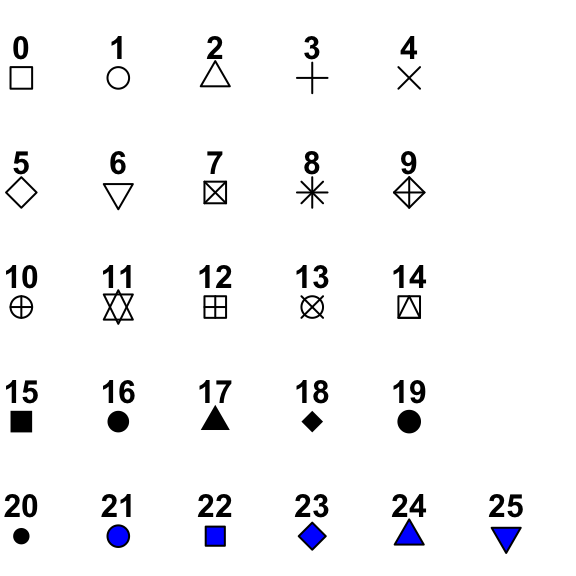
\includegraphics[width=0.4\linewidth]{images/04-points-symbols} 

}

\caption{An illustration of the different point shapes commonly used in R. The default is number 19, but this can be changed using the `shape = x` parameter, where x is the shape number.}\label{fig:points-symbols}
\end{figure}

We could decide that we do not want filled circles as our points. There are 25 different shapes (see Figure \ref{fig:points-symbols}). The default is number 19, which is a single-coloured dot, but we could choose any of the shapes - for example, shape number 3 is a plus sign.

\begin{Shaded}
\begin{Highlighting}[]
\NormalTok{ggplot2}\SpecialCharTok{::}\FunctionTok{ggplot}\NormalTok{(iris, }\FunctionTok{aes}\NormalTok{(}\AttributeTok{x =}\NormalTok{ Sepal.Length, }\AttributeTok{y =}\NormalTok{ Sepal.Width)) }\SpecialCharTok{+}
  \FunctionTok{geom\_point}\NormalTok{(}\FunctionTok{aes}\NormalTok{(}\AttributeTok{colour =}\NormalTok{ Species), }\AttributeTok{shape =} \DecValTok{3}\NormalTok{)}
\end{Highlighting}
\end{Shaded}

\pandocbounded{\includegraphics[keepaspectratio]{_main_files/figure-latex/unnamed-chunk-102-1.pdf}}

It is also possible to make the shape change depending on data within the dataset as an aesthetic or to use any single letter or character from your keyboard instead of one of the preset shapes (try these as an exercise). Finally, the size of each point is not fixed and can be changed in a similar way. As a default, the points are size 1.5, but it is possible to change that number to any positive number. Below, we show an example where we have increased the point size to 3.

\begin{Shaded}
\begin{Highlighting}[]
\NormalTok{ggplot2}\SpecialCharTok{::}\FunctionTok{ggplot}\NormalTok{(iris, }\FunctionTok{aes}\NormalTok{(}\AttributeTok{x =}\NormalTok{ Sepal.Length, }\AttributeTok{y =}\NormalTok{ Sepal.Width)) }\SpecialCharTok{+}
  \FunctionTok{geom\_point}\NormalTok{(}\FunctionTok{aes}\NormalTok{(}\AttributeTok{colour =}\NormalTok{ Species), }\AttributeTok{size =} \DecValTok{3}\NormalTok{)}
\end{Highlighting}
\end{Shaded}

\textbf{Editing the plot layer:}
1. What happens if you make size an aesthetic based on petal width?
2. Shapes 21-25 can take two colours, a ``colour'' for the edges and a ``fill'' for the centre. Can you work out how to add your choice of fill?
3. Can you change the shape of the points based on the species of iris?
4. Try to make all the shapes a letter of your choice - remember to include the character within quotation marks.

\subsection{Facets}\label{facets}

Facets split the single graph into separate but linked graphs by a given grouping. For larger datasets, this can be split into a grid by two different groupings, but for our example, we will just split by the different iris species, like we have done by colour. We can either define this split by defining which grouping sets the rows and/or columns, using \textbf{\texttt{cols\ =\ vars(group)}} / \textbf{\texttt{rows\ =\ vars(group)}}, or it can be defined with an equation \textbf{\texttt{.\textasciitilde{}\ group}} / \textbf{\texttt{group\textasciitilde{}.}} / \textbf{\texttt{group1\textasciitilde{}\ group2}}. See Table \ref{tab:precedence} for tilde definition and will be covered further in Section \ref{sec:simpleLinearRegression}. Examples of both options for the iris dataset are below:

Example 1

\begin{Shaded}
\begin{Highlighting}[]
\NormalTok{ggplot2}\SpecialCharTok{::}\FunctionTok{ggplot}\NormalTok{(iris, }\FunctionTok{aes}\NormalTok{(}\AttributeTok{x =}\NormalTok{ Sepal.Length, }\AttributeTok{y =}\NormalTok{ Sepal.Width)) }\SpecialCharTok{+}
  \FunctionTok{geom\_point}\NormalTok{(}\FunctionTok{aes}\NormalTok{(}\AttributeTok{colour =}\NormalTok{ Species), }\AttributeTok{size =} \DecValTok{3}\NormalTok{) }\SpecialCharTok{+}
  \FunctionTok{facet\_grid}\NormalTok{(}\AttributeTok{cols =} \FunctionTok{vars}\NormalTok{(Species))}
\end{Highlighting}
\end{Shaded}

\pandocbounded{\includegraphics[keepaspectratio]{_main_files/figure-latex/unnamed-chunk-104-1.pdf}}

Example 2

\begin{Shaded}
\begin{Highlighting}[]
\NormalTok{ggplot2}\SpecialCharTok{::}\FunctionTok{ggplot}\NormalTok{(iris, }\FunctionTok{aes}\NormalTok{(}\AttributeTok{x =}\NormalTok{ Sepal.Length, }\AttributeTok{y =}\NormalTok{ Sepal.Width)) }\SpecialCharTok{+}
  \FunctionTok{geom\_point}\NormalTok{(}\FunctionTok{aes}\NormalTok{(}\AttributeTok{colour =}\NormalTok{ Species), }\AttributeTok{size =} \DecValTok{3}\NormalTok{) }\SpecialCharTok{+}
  \FunctionTok{facet\_grid}\NormalTok{(.}\SpecialCharTok{\textasciitilde{}}\NormalTok{Species)}
\end{Highlighting}
\end{Shaded}

\pandocbounded{\includegraphics[keepaspectratio]{_main_files/figure-latex/unnamed-chunk-105-1.pdf}}

\textbf{Facet options:}
1. What happens if you set \textbf{\texttt{scales\ =\ "free\_x"}} or \textbf{\texttt{scales\ =\ "free\_y"}} or \textbf{\texttt{scales\ =\ "free"}}?
2. What happens if you try the same arguments with \textbf{\texttt{space}}?
3. Is \textbf{\texttt{cols\ =\ vars(Species)}} equivalent to \textbf{\texttt{.\textasciitilde{}Species}} or \textbf{\texttt{Species\textasciitilde{}.}}?

\subsection{Making it all look pretty}\label{making-it-all-look-pretty}

\subsubsection{Background and theme}\label{background-and-theme}

All plots up to this point were created using ggplot's default theme. You can change this to alter the plot background. Below, I will give you a few examples of this. You can also click here to explore more of the themes: \url{https://ggplot2.tidyverse.org/reference/ggtheme.html}. Below is the first plot, which shows the default theme for ggplot2 graphs.

\begin{Shaded}
\begin{Highlighting}[]
\NormalTok{ggplot2}\SpecialCharTok{::}\FunctionTok{ggplot}\NormalTok{(iris, }\FunctionTok{aes}\NormalTok{(}\AttributeTok{x =}\NormalTok{ Sepal.Length, }\AttributeTok{y =}\NormalTok{ Sepal.Width)) }\SpecialCharTok{+}
  \FunctionTok{geom\_point}\NormalTok{(}\FunctionTok{aes}\NormalTok{(}\AttributeTok{colour =}\NormalTok{ Species), }\AttributeTok{size =} \DecValTok{3}\NormalTok{) }
\end{Highlighting}
\end{Shaded}

\pandocbounded{\includegraphics[keepaspectratio]{_main_files/figure-latex/unnamed-chunk-106-1.pdf}}

Below is the second plot, which shows the black and white theme for ggplot2 graphs. The plot now has a white background with grid markers.

\begin{Shaded}
\begin{Highlighting}[]
\NormalTok{ggplot2}\SpecialCharTok{::}\FunctionTok{ggplot}\NormalTok{(iris, }\FunctionTok{aes}\NormalTok{(}\AttributeTok{x =}\NormalTok{ Sepal.Length, }\AttributeTok{y =}\NormalTok{ Sepal.Width)) }\SpecialCharTok{+}
  \FunctionTok{geom\_point}\NormalTok{(}\FunctionTok{aes}\NormalTok{(}\AttributeTok{colour =}\NormalTok{ Species), }\AttributeTok{size =} \DecValTok{3}\NormalTok{)}\SpecialCharTok{+}
  \FunctionTok{theme\_bw}\NormalTok{()}
\end{Highlighting}
\end{Shaded}

\pandocbounded{\includegraphics[keepaspectratio]{_main_files/figure-latex/unnamed-chunk-107-1.pdf}}

Below is the third plot, which illustrates the classic theme for ggplot2 graphs. The plot now has a white background and no grid markers.

\begin{Shaded}
\begin{Highlighting}[]
\NormalTok{ggplot2}\SpecialCharTok{::}\FunctionTok{ggplot}\NormalTok{(iris, }\FunctionTok{aes}\NormalTok{(}\AttributeTok{x =}\NormalTok{ Sepal.Length, }\AttributeTok{y =}\NormalTok{ Sepal.Width)) }\SpecialCharTok{+}
  \FunctionTok{geom\_point}\NormalTok{(}\FunctionTok{aes}\NormalTok{(}\AttributeTok{colour =}\NormalTok{ Species), }\AttributeTok{size =} \DecValTok{3}\NormalTok{)}\SpecialCharTok{+}
  \FunctionTok{theme\_classic}\NormalTok{()}
\end{Highlighting}
\end{Shaded}

\pandocbounded{\includegraphics[keepaspectratio]{_main_files/figure-latex/unnamed-chunk-108-1.pdf}}

Below is the fourth plot, which shows the dark theme for ggplot2 graphs.

\begin{Shaded}
\begin{Highlighting}[]
\NormalTok{ggplot2}\SpecialCharTok{::}\FunctionTok{ggplot}\NormalTok{(iris, }\FunctionTok{aes}\NormalTok{(}\AttributeTok{x =}\NormalTok{ Sepal.Length, }\AttributeTok{y =}\NormalTok{ Sepal.Width)) }\SpecialCharTok{+}
  \FunctionTok{geom\_point}\NormalTok{(}\FunctionTok{aes}\NormalTok{(}\AttributeTok{colour =}\NormalTok{ Species), }\AttributeTok{size =} \DecValTok{3}\NormalTok{)}\SpecialCharTok{+}
  \FunctionTok{theme\_dark}\NormalTok{()}
\end{Highlighting}
\end{Shaded}

\pandocbounded{\includegraphics[keepaspectratio]{_main_files/figure-latex/unnamed-chunk-109-1.pdf}}

Below is the fifth plot, which shows all of the themes we have covered so far - this includes the default, bw, classic and dark. These were plotted together using another R package that we will discuss further on.

\begin{Shaded}
\begin{Highlighting}[]
\FunctionTok{library}\NormalTok{(patchwork)}
\NormalTok{p\_base}\OtherTok{\textless{}{-}}\NormalTok{ ggplot2}\SpecialCharTok{::}\FunctionTok{ggplot}\NormalTok{(iris, }\FunctionTok{aes}\NormalTok{(}\AttributeTok{x =}\NormalTok{ Sepal.Length,}\AttributeTok{y =}\NormalTok{ Sepal.Width))}\SpecialCharTok{+}
  \FunctionTok{geom\_point}\NormalTok{(}\FunctionTok{aes}\NormalTok{(}\AttributeTok{color =}\NormalTok{ Species), }\AttributeTok{size =} \DecValTok{3}\NormalTok{)}

\CommentTok{\# shows all of the plots together using Patchwork Package}
\NormalTok{p1 }\OtherTok{\textless{}{-}}\NormalTok{ p\_base }\SpecialCharTok{+} \FunctionTok{ggtitle}\NormalTok{(}\StringTok{"Default Theme"}\NormalTok{) }\SpecialCharTok{+} 
  \FunctionTok{theme}\NormalTok{(}\AttributeTok{legend.position =} \StringTok{"none"}\NormalTok{)}
\NormalTok{p2 }\OtherTok{\textless{}{-}}\NormalTok{ p\_base }\SpecialCharTok{+} \FunctionTok{theme\_bw}\NormalTok{() }\SpecialCharTok{+} \FunctionTok{ggtitle}\NormalTok{(}\StringTok{"Theme\_bw()"}\NormalTok{) }\SpecialCharTok{+} 
  \FunctionTok{theme}\NormalTok{(}\AttributeTok{legend.position =} \StringTok{"right"}\NormalTok{)}
\NormalTok{p3 }\OtherTok{\textless{}{-}}\NormalTok{ p\_base }\SpecialCharTok{+} \FunctionTok{theme\_classic}\NormalTok{() }\SpecialCharTok{+} \FunctionTok{ggtitle}\NormalTok{(}\StringTok{"Theme\_classic()"}\NormalTok{)}\SpecialCharTok{+} 
  \FunctionTok{theme}\NormalTok{(}\AttributeTok{legend.position =} \StringTok{"none"}\NormalTok{)}
\NormalTok{p4 }\OtherTok{\textless{}{-}}\NormalTok{ p\_base }\SpecialCharTok{+} \FunctionTok{theme\_dark}\NormalTok{() }\SpecialCharTok{+} \FunctionTok{ggtitle}\NormalTok{(}\StringTok{"Theme\_dark()"}\NormalTok{)}\SpecialCharTok{+} 
  \FunctionTok{theme}\NormalTok{(}\AttributeTok{legend.position =} \StringTok{"right"}\NormalTok{)}

\CommentTok{\# patchwork}
\NormalTok{(p1}\SpecialCharTok{|}\NormalTok{p2)}\SpecialCharTok{/}\NormalTok{(p3}\SpecialCharTok{|}\NormalTok{p4)}
\end{Highlighting}
\end{Shaded}

\pandocbounded{\includegraphics[keepaspectratio]{_main_files/figure-latex/unnamed-chunk-110-1.pdf}}

Below is a plot that highlights how you can manually change the panel background, plot background and other elements, including the line colour (major and minor), and the axes text colour.

\begin{Shaded}
\begin{Highlighting}[]
\NormalTok{ggplot2}\SpecialCharTok{::}\FunctionTok{ggplot}\NormalTok{(iris, }\FunctionTok{aes}\NormalTok{(Sepal.Length, Sepal.Width)) }\SpecialCharTok{+}
  \FunctionTok{geom\_point}\NormalTok{() }\SpecialCharTok{+}
  \FunctionTok{theme}\NormalTok{(}
    \AttributeTok{panel.background =} \FunctionTok{element\_rect}\NormalTok{(}\AttributeTok{fill =} \StringTok{"hotpink"}\NormalTok{),}
    \AttributeTok{plot.background =} \FunctionTok{element\_rect}\NormalTok{(}\AttributeTok{fill =} \StringTok{"skyblue"}\NormalTok{),}
    \AttributeTok{panel.grid.major =} \FunctionTok{element\_line}\NormalTok{(}\AttributeTok{color =} \StringTok{"brown"}\NormalTok{,}
                                    \AttributeTok{linewidth =} \DecValTok{1}\NormalTok{),}
    \AttributeTok{panel.grid.minor =} \FunctionTok{element\_line}\NormalTok{(}\AttributeTok{color =} \StringTok{"limegreen"}\NormalTok{, }
                                    \AttributeTok{linewidth =} \FloatTok{0.5}\NormalTok{),}
    \AttributeTok{text =} \FunctionTok{element\_text}\NormalTok{(}\AttributeTok{color =} \StringTok{"purple"}\NormalTok{)}
\NormalTok{  )}
\end{Highlighting}
\end{Shaded}

\pandocbounded{\includegraphics[keepaspectratio]{_main_files/figure-latex/unnamed-chunk-111-1.pdf}}

\textbf{Background and theme options:}
1. Look up other themes. What is your favourite theme which you might use by default?
2. Can you use the different theme options in the last example to make a theme based on your favourite film (ours may draw inspiration from Barbie)?

\subsubsection{Renaming axes}\label{renaming-axes}

By default, ggplot2 uses the column names used in the aesthetic calls to name the axes; however, that is not always the most useful. In our examples so far, the x-axis has been labelled \textbf{\texttt{"Sepal.Length"}} and the y-axis has been labelled \textbf{\texttt{"Sepal.Width"}}. Whilst this is sufficient to describe the data, it could be more descriptive. We can easily rename the axes in ggplot2 using the \textbf{\texttt{labs}} layer. Within \textbf{\texttt{labs}} we can change either of the axes, and we can also add a title to the plot and adjust the title of the legend. Note that to change the title of the legend, you have to refer to it as the aesthetic (e.g.~\textbf{\texttt{colour}} or \textbf{\texttt{fill}}).

You can also use additional functions to make further edits. Here we will demonstrate the function \texttt{scale\_x\_continuous()} which can change aspects of the x-axis. It has an analogous function (\texttt{scale\_y\_continuous()}) that does the same for the y-axis. We are defining three aspects within \texttt{scale\_x\_continuous()}: the breaks, the labels, and the limits. The breaks tell ggplot2 where to place the tick labels. Without any further adjustment, the numbers in breaks will define both the position and the label for each tick. Labels adjust what is written at each tick mark. We have changed the labels from integer numbers to \textbf{\texttt{"four,\ five,\ six,\ seven,\ and\ eight"}}. The limits enable us to define how long we want the axes to be. This can be wider than the data, meaning that there is empty space outside of the data, or can be thinner than the data, meaning some data are not visualised. In the following, we have slightly extended the axes in both directions using \textbf{\texttt{limits\ =\ c(3.5,8.5)}}.

\begin{Shaded}
\begin{Highlighting}[]
\NormalTok{ggplot2}\SpecialCharTok{::}\FunctionTok{ggplot}\NormalTok{(iris, }\FunctionTok{aes}\NormalTok{(}\AttributeTok{x =}\NormalTok{ Sepal.Length, }\AttributeTok{y =}\NormalTok{ Sepal.Width))}\SpecialCharTok{+}
  \FunctionTok{geom\_point}\NormalTok{(}\FunctionTok{aes}\NormalTok{(}\AttributeTok{color =}\NormalTok{ Species))}\SpecialCharTok{+}
  \FunctionTok{labs}\NormalTok{(}\AttributeTok{title =} \StringTok{"Sepal Dimensions in Iris Dataset"}\NormalTok{,}
       \AttributeTok{x =} \StringTok{"Sepal Length (cm)"}\NormalTok{,}
       \AttributeTok{y =} \StringTok{"Sepal Width (cm)"}\NormalTok{, }
       \AttributeTok{color =} \StringTok{"Iris Species"}\NormalTok{)}\SpecialCharTok{+}
  \FunctionTok{scale\_x\_continuous}\NormalTok{(}\AttributeTok{breaks =} \FunctionTok{c}\NormalTok{(}\DecValTok{4}\NormalTok{, }\DecValTok{5}\NormalTok{, }\DecValTok{6}\NormalTok{, }\DecValTok{7}\NormalTok{, }\DecValTok{8}\NormalTok{),}
                     \AttributeTok{labels =} \FunctionTok{c}\NormalTok{(}\StringTok{"Four"}\NormalTok{, }\StringTok{"Five"}\NormalTok{, }\StringTok{"Six"}\NormalTok{, }\StringTok{"Seven"}\NormalTok{, }\StringTok{"Eight"}\NormalTok{),}
                     \AttributeTok{limits =} \FunctionTok{c}\NormalTok{(}\FloatTok{3.5}\NormalTok{,}\FloatTok{8.5}\NormalTok{)) }\SpecialCharTok{+} 
  \FunctionTok{theme\_bw}\NormalTok{()}
\end{Highlighting}
\end{Shaded}

\pandocbounded{\includegraphics[keepaspectratio]{_main_files/figure-latex/unnamed-chunk-112-1.pdf}}

\textbf{Axes options:}
1. Can you shrink the x-axis so that only data between 5 and 7cm are shown?
2. Can you increase the y-axis to include negative numbers?
3. Can you change the title of the plot and the legend?

\subsection{Different Types of Plots}\label{different-types-of-plots}

Here we have several types of plots that are useful for visualising different types of data.

\subsubsection{Histogram}\label{histogram}

Histograms are useful for showing the distribution of a single numeric variable. This version shows the bars side by side by species within each bin, making it easier to directly compare counts for each species.

\textbf{Layout in histograms:}
Look at the plot below
1. What happens if you change the \textbf{\texttt{position}} argument from `dodge' to `stack'?
2. Change the \textbf{\texttt{binwidth}} to values between 0.2 and 1.5 - what is the most useful binwidth?
3. If you change the \textbf{\texttt{position}} from `dodge' to `identity' the bars should all overlap - can you change the alpha value or the fill and colour values to make it clearer how they overlap?

\begin{Shaded}
\begin{Highlighting}[]
\NormalTok{ggplot2}\SpecialCharTok{::}\FunctionTok{ggplot}\NormalTok{(iris, }\FunctionTok{aes}\NormalTok{(}\AttributeTok{x =}\NormalTok{ Sepal.Length, }\AttributeTok{fill =}\NormalTok{ Species)) }\SpecialCharTok{+} 
  \FunctionTok{geom\_histogram}\NormalTok{(}\AttributeTok{binwidth =} \FloatTok{0.6}\NormalTok{, }
                 \AttributeTok{color =} \StringTok{\textquotesingle{}black\textquotesingle{}}\NormalTok{, }\AttributeTok{alpha =} \FloatTok{0.8}\NormalTok{, }\AttributeTok{position =} \StringTok{\textquotesingle{}dodge\textquotesingle{}}\NormalTok{)}\SpecialCharTok{+}
  \FunctionTok{labs}\NormalTok{(}\AttributeTok{title =} \StringTok{"Dodged Histogram of Sepal Length by Species"}\NormalTok{)}\SpecialCharTok{+}
  \FunctionTok{theme}\NormalTok{(}\AttributeTok{plot.title =} \FunctionTok{element\_text}\NormalTok{(}\AttributeTok{size =} \DecValTok{16}\NormalTok{, }\AttributeTok{face =} \StringTok{"bold"}\NormalTok{))}
\end{Highlighting}
\end{Shaded}

\pandocbounded{\includegraphics[keepaspectratio]{_main_files/figure-latex/unnamed-chunk-113-1.pdf}}

\subsubsection{Box plots}\label{box-plots}

Box plots are great for visualising the spread of data and identifying outliers in continuous data across categories.

\begin{Shaded}
\begin{Highlighting}[]
\NormalTok{ggplot2}\SpecialCharTok{::}\FunctionTok{ggplot}\NormalTok{(iris, }\FunctionTok{aes}\NormalTok{(}\AttributeTok{x =}\NormalTok{ Species, }
                          \AttributeTok{y =}\NormalTok{ Sepal.Length, }
                          \AttributeTok{fill =}\NormalTok{ Species))}\SpecialCharTok{+}
  \FunctionTok{geom\_boxplot}\NormalTok{(}\AttributeTok{color =} \StringTok{\textquotesingle{}black\textquotesingle{}}\NormalTok{, }\AttributeTok{alpha =} \FloatTok{0.8}\NormalTok{)}\SpecialCharTok{+}
  \FunctionTok{labs}\NormalTok{(}\AttributeTok{title =} \StringTok{"Boxplot of Sepal Length by Species"}\NormalTok{)}\SpecialCharTok{+}
  \FunctionTok{theme}\NormalTok{(}\AttributeTok{plot.title =} \FunctionTok{element\_text}\NormalTok{(}\AttributeTok{size =} \DecValTok{16}\NormalTok{, }\AttributeTok{face =} \StringTok{"bold"}\NormalTok{))}
\end{Highlighting}
\end{Shaded}

\pandocbounded{\includegraphics[keepaspectratio]{_main_files/figure-latex/unnamed-chunk-114-1.pdf}}

\textbf{Layout in box plots:}
1. Can you make the lines in the box plot turn the same colour as the box fill? Why is this not the best of ideas?
2. If you decide the lines are too thin, you can add in an argument (not an aesthetic) to \textbf{\texttt{geom\_boxplot}} called \textbf{\texttt{linewidth}}.

\subsubsection{Scatter plots}\label{scatter-plots}

These are ideal for showing relationships between two continuous variables.

\begin{Shaded}
\begin{Highlighting}[]
\NormalTok{ggplot2}\SpecialCharTok{::}\FunctionTok{ggplot}\NormalTok{(iris, }\FunctionTok{aes}\NormalTok{(}\AttributeTok{x =}\NormalTok{ Sepal.Length, }\AttributeTok{y =}\NormalTok{ Sepal.Width)) }\SpecialCharTok{+}
  \FunctionTok{geom\_point}\NormalTok{(}\FunctionTok{aes}\NormalTok{(}\AttributeTok{colour =}\NormalTok{ Species), }\AttributeTok{size =} \DecValTok{3}\NormalTok{) }\SpecialCharTok{+}
  \FunctionTok{labs}\NormalTok{(}\AttributeTok{title =} \StringTok{"Scatter plot of Sepal Length/Width by Species"}\NormalTok{)}\SpecialCharTok{+}
  \FunctionTok{theme}\NormalTok{(}\AttributeTok{plot.title =} \FunctionTok{element\_text}\NormalTok{(}\AttributeTok{size =} \DecValTok{16}\NormalTok{, }\AttributeTok{face =} \StringTok{"bold"}\NormalTok{))}
\end{Highlighting}
\end{Shaded}

\pandocbounded{\includegraphics[keepaspectratio]{_main_files/figure-latex/unnamed-chunk-115-1.pdf}}

\subsubsection{Bar Charts}\label{bar-charts}

Bar charts are used for comparing quantities across discrete categories.

\begin{Shaded}
\begin{Highlighting}[]
\NormalTok{iris\_means }\OtherTok{\textless{}{-}}\NormalTok{ stats}\SpecialCharTok{::}\FunctionTok{aggregate}\NormalTok{(Sepal.Length }\SpecialCharTok{\textasciitilde{}}\NormalTok{ Species, }
                               \AttributeTok{data =}\NormalTok{ iris, }\AttributeTok{FUN =}\NormalTok{ mean)}

\NormalTok{ggplot2}\SpecialCharTok{::}\FunctionTok{ggplot}\NormalTok{(iris\_means, }\FunctionTok{aes}\NormalTok{(}\AttributeTok{x =}\NormalTok{ Species, }
                                \AttributeTok{y =}\NormalTok{ Sepal.Length, }
                                \AttributeTok{fill =}\NormalTok{ Species)) }\SpecialCharTok{+}
  \FunctionTok{geom\_col}\NormalTok{(}\AttributeTok{color =} \StringTok{\textquotesingle{}black\textquotesingle{}}\NormalTok{, }\AttributeTok{alpha =} \FloatTok{0.8}\NormalTok{) }\SpecialCharTok{+}
  \FunctionTok{labs}\NormalTok{(}\AttributeTok{title =} \StringTok{"Mean Sepal Length per Species"}\NormalTok{, }
       \AttributeTok{y =} \StringTok{"Mean Sepal Length"}\NormalTok{) }\SpecialCharTok{+}
  \FunctionTok{theme}\NormalTok{(}\AttributeTok{plot.title =} \FunctionTok{element\_text}\NormalTok{(}\AttributeTok{size =} \DecValTok{16}\NormalTok{, }\AttributeTok{face =} \StringTok{"bold"}\NormalTok{))}
\end{Highlighting}
\end{Shaded}

\pandocbounded{\includegraphics[keepaspectratio]{_main_files/figure-latex/unnamed-chunk-116-1.pdf}}

\subsubsection{Bar Charts with Error Bars}\label{bar-charts-with-error-bars}

Here we include error bars. Error bars are graphical representations of the variability or uncertainty in the data. They provide insights into the precision of measurements or the confidence in estimates like means. In bar charts, adding error bars can help people to understand the range within which the true value likely falls.

For example, when plotting the mean Sepal Length by species in the iris dataset, we can add error bars to show the \textbf{\hyperref[acronyms_SD]{SD}} or \textbf{\hyperref[acronyms_SE]{SE}} within each species group.

\begin{Shaded}
\begin{Highlighting}[]
\NormalTok{base}\SpecialCharTok{::}\FunctionTok{library}\NormalTok{(dplyr)}
\NormalTok{iris\_summary }\OtherTok{\textless{}{-}}\NormalTok{ iris }\SpecialCharTok{\%\textgreater{}\%}\NormalTok{ dplyr}\SpecialCharTok{::}\FunctionTok{group\_by}\NormalTok{(Species) }\SpecialCharTok{\%\textgreater{}\%} 
\NormalTok{  dplyr}\SpecialCharTok{::}\FunctionTok{summarise}\NormalTok{(}\AttributeTok{mean\_sepal =}\NormalTok{ base}\SpecialCharTok{::}\FunctionTok{mean}\NormalTok{(Sepal.Length),}
                   \AttributeTok{se\_sepal =}\NormalTok{ stats}\SpecialCharTok{::}\FunctionTok{sd}\NormalTok{(Sepal.Length) }\SpecialCharTok{/}\NormalTok{base}\SpecialCharTok{::}\FunctionTok{sqrt}\NormalTok{(}\FunctionTok{n}\NormalTok{()))}
\end{Highlighting}
\end{Shaded}

\begin{Shaded}
\begin{Highlighting}[]
\NormalTok{ggplot2}\SpecialCharTok{::}\FunctionTok{ggplot}\NormalTok{(iris\_summary, }\FunctionTok{aes}\NormalTok{(}\AttributeTok{x =}\NormalTok{ Species, }\AttributeTok{y =}\NormalTok{ mean\_sepal, }\AttributeTok{fill =}\NormalTok{ Species)) }\SpecialCharTok{+} 
  \FunctionTok{geom\_col}\NormalTok{(}\AttributeTok{color =} \StringTok{\textquotesingle{}black\textquotesingle{}}\NormalTok{, }\AttributeTok{alpha =} \FloatTok{0.8}\NormalTok{) }\SpecialCharTok{+} 
  \FunctionTok{geom\_errorbar}\NormalTok{(}\FunctionTok{aes}\NormalTok{(}\AttributeTok{ymin =}\NormalTok{ mean\_sepal }\SpecialCharTok{{-}}\NormalTok{ se\_sepal, }
                    \AttributeTok{ymax =}\NormalTok{ mean\_sepal }\SpecialCharTok{+}\NormalTok{ se\_sepal), }
                \AttributeTok{width =} \FloatTok{0.2}\NormalTok{, }\AttributeTok{color =} \StringTok{"black"}\NormalTok{) }\SpecialCharTok{+}
  \FunctionTok{labs}\NormalTok{(}\AttributeTok{title =} \StringTok{"Mean Sepal Length per Species with **}\SpecialCharTok{\textbackslash{}a}\StringTok{cr\{SE\}**"}\NormalTok{, }
       \AttributeTok{y =} \StringTok{"Mean Sepal Length"}\NormalTok{) }\SpecialCharTok{+}
  \FunctionTok{theme}\NormalTok{(}\AttributeTok{plot.title =} \FunctionTok{element\_text}\NormalTok{(}\AttributeTok{size =} \DecValTok{16}\NormalTok{, }\AttributeTok{face =} \StringTok{"bold"}\NormalTok{))}
\end{Highlighting}
\end{Shaded}

\begin{verbatim}
## Warning in grid.Call(C_textBounds, as.graphicsAnnot(x$label), x$x, x$y, : font
## width unknown for character 0x07 in encoding cp1252
\end{verbatim}

\begin{verbatim}
## Warning in grid.Call.graphics(C_text, as.graphicsAnnot(x$label), x$x, x$y, :
## font width unknown for character 0x07 in encoding cp1252
\end{verbatim}

\pandocbounded{\includegraphics[keepaspectratio]{_main_files/figure-latex/unnamed-chunk-118-1.pdf}}

\subsubsection{Faceted Plots}\label{sec:facetedPlots}

Here, we can break the data into subsets and plot each subset in its own panel for comparison.

\begin{Shaded}
\begin{Highlighting}[]
\NormalTok{ggplot2}\SpecialCharTok{::}\FunctionTok{ggplot}\NormalTok{(iris, }\FunctionTok{aes}\NormalTok{(}\AttributeTok{x =}\NormalTok{ Sepal.Length, }\AttributeTok{y =}\NormalTok{ Sepal.Width, }\AttributeTok{fill =}\NormalTok{ Species))}\SpecialCharTok{+} 
  \FunctionTok{geom\_point}\NormalTok{(}\AttributeTok{shape =} \DecValTok{21}\NormalTok{, }\AttributeTok{color =} \StringTok{\textquotesingle{}black\textquotesingle{}}\NormalTok{, }\AttributeTok{size =} \DecValTok{2}\NormalTok{)}\SpecialCharTok{+}
  \FunctionTok{facet\_wrap}\NormalTok{(}\SpecialCharTok{\textasciitilde{}}\NormalTok{Species)}\SpecialCharTok{+}
  \FunctionTok{labs}\NormalTok{(}\AttributeTok{title =} \StringTok{"Sepal Length vs Width by Species"}\NormalTok{, }
       \AttributeTok{x =} \StringTok{"Sepal Length"}\NormalTok{, }\AttributeTok{y =} \StringTok{"Sepal Width"}\NormalTok{)}\SpecialCharTok{+}
  \FunctionTok{theme}\NormalTok{(}\AttributeTok{plot.title =} \FunctionTok{element\_text}\NormalTok{(}\AttributeTok{size =} \DecValTok{16}\NormalTok{, }\AttributeTok{face =} \StringTok{"bold"}\NormalTok{),}
        \AttributeTok{strip.text =} \FunctionTok{element\_text}\NormalTok{(}\AttributeTok{face =} \StringTok{"bold"}\NormalTok{))}
\end{Highlighting}
\end{Shaded}

\pandocbounded{\includegraphics[keepaspectratio]{_main_files/figure-latex/unnamed-chunk-119-1.pdf}}

\subsubsection{Viridis Colour Palettes}\label{viridis-colour-palettes}

This is an example of how you can use a colour palette in R. Further examples using the \texttt{viridis} package can be found here.

\begin{Shaded}
\begin{Highlighting}[]
\CommentTok{\#base::library(ggplot2)}
\CommentTok{\#base::library(viridis)}
\NormalTok{ggplot2}\SpecialCharTok{::}\FunctionTok{ggplot}\NormalTok{(iris, }\FunctionTok{aes}\NormalTok{(}\AttributeTok{x =}\NormalTok{ Sepal.Length, }\AttributeTok{y =}\NormalTok{ Sepal.Width, }\AttributeTok{fill =}\NormalTok{ Species)) }\SpecialCharTok{+}
  \FunctionTok{geom\_point}\NormalTok{(}\AttributeTok{shape =} \DecValTok{21}\NormalTok{, }\AttributeTok{color =} \StringTok{"black"}\NormalTok{, }\AttributeTok{size =} \DecValTok{2}\NormalTok{) }\SpecialCharTok{+}
  \FunctionTok{facet\_wrap}\NormalTok{(}\SpecialCharTok{\textasciitilde{}}\NormalTok{ Species) }\SpecialCharTok{+}
  \FunctionTok{scale\_fill\_viridis}\NormalTok{(}\AttributeTok{option =} \StringTok{"plasma"}\NormalTok{, }\AttributeTok{discrete =}\NormalTok{ T) }\SpecialCharTok{+}  
  \FunctionTok{labs}\NormalTok{(}\AttributeTok{title =} \StringTok{"Sepal Length vs Width by Species with Viridis Palette"}\NormalTok{,}
       \AttributeTok{x =} \StringTok{"Sepal Length"}\NormalTok{, }\AttributeTok{y =} \StringTok{"Sepal Width"}\NormalTok{)  }\SpecialCharTok{+}
  \FunctionTok{theme}\NormalTok{(}\AttributeTok{plot.title =} \FunctionTok{element\_text}\NormalTok{(}\AttributeTok{size =} \DecValTok{18}\NormalTok{, }\AttributeTok{face =} \StringTok{"bold"}\NormalTok{),}
        \AttributeTok{strip.text =} \FunctionTok{element\_text}\NormalTok{(}\AttributeTok{face =} \StringTok{"bold"}\NormalTok{, }\AttributeTok{size =} \DecValTok{12}\NormalTok{))}
\end{Highlighting}
\end{Shaded}

\section{Individualising your plots}\label{individualising-your-plots}

\subsection{Colours}\label{colours}

We have already shown an example of the viridis colour palette. This set of palettes is designed to be printer and colour-blind friendly. In the example above, we used the ``plasma'' palette for a discrete selection of data, but all palettes are continuous, and the default for the functions \texttt{scale\_fill\_viridis()} and \texttt{scale\_colour\_viridis()} are for continuous data. More details on the different palettes available through viridis are available here: \url{https://cran.r-project.org/web/packages/viridis/vignettes/intro-to-viridis.html\#the-color-scales}.

Another similar package that provides different palettes is RColorBrewer. Within ggplot, this can be called, similar to viridis, with the functions \texttt{scale\_colour\_brewer()} and \texttt{scale\_fill\_brewer()}. More information about the colour palettes from RColorBrewer are available here: \url{https://colorbrewer2.org}

Sometimes, you just want to define your own palette for plots, and there are many different packages and resources to help select colours. Some of our favourites include:

\begin{enumerate}
\def\labelenumi{\arabic{enumi}.}
\tightlist
\item
  MetBrewer (\url{https://www.blakerobertmills.com/my-work/met-brewer}) - palettes based on objects in the Metropolitan Museum of Art in New York
\item
  coolors (\url{https://coolors.co/generate}) - generates new palettes with the click of a space bar
\item
  PNWColors (\url{https://github.com/jakelawlor/PNWColors}) - palettes based on Washington state and the Pacific Northwest of the USA
\item
  WesAnderson (\url{https://github.com/karthik/wesanderson}) - palettes based on Wes Anderson films
\end{enumerate}

It is also worth checking that any palettes you choose are colour-blind friendly. RColorBrewer, viridis, and coolors all are, or have options to easily check, but if you are selecting from other packages or choosing colours by hand, you can use the package colorblindcheck.

To colour sections with your own colours, not from a palette, you need to first define your palette and then use \texttt{scale\_fill\_manual()} or \texttt{scale\_colour\_manual()}, as shown below:

\begin{Shaded}
\begin{Highlighting}[]
\NormalTok{SpecCols }\OtherTok{\textless{}{-}} \FunctionTok{c}\NormalTok{(}\AttributeTok{setosa =} \StringTok{"\#A3D9FF"}\NormalTok{, }\AttributeTok{versicolor =} \StringTok{"\#7E6B8F"}\NormalTok{, }\AttributeTok{virginica =} \StringTok{"\#96E6B3"}\NormalTok{)}
\NormalTok{ggplot2}\SpecialCharTok{::}\FunctionTok{ggplot}\NormalTok{(iris, }\FunctionTok{aes}\NormalTok{(}\AttributeTok{x =}\NormalTok{ Sepal.Length, }\AttributeTok{y =}\NormalTok{ Sepal.Width, }\AttributeTok{colour =}\NormalTok{ Species)) }\SpecialCharTok{+}
  \FunctionTok{geom\_point}\NormalTok{(}\AttributeTok{size  =} \DecValTok{3}\NormalTok{) }\SpecialCharTok{+}
  \FunctionTok{scale\_colour\_manual}\NormalTok{(}\AttributeTok{values =}\NormalTok{ SpecCols) }\SpecialCharTok{+}  
  \FunctionTok{labs}\NormalTok{(}\AttributeTok{x =} \StringTok{"Sepal Length"}\NormalTok{, }\AttributeTok{y =} \StringTok{"Sepal Width"}\NormalTok{)  }\SpecialCharTok{+}
  \FunctionTok{theme\_light}\NormalTok{() }\SpecialCharTok{+}
  \FunctionTok{theme}\NormalTok{(}\AttributeTok{plot.title =} \FunctionTok{element\_text}\NormalTok{(}\AttributeTok{size =} \DecValTok{18}\NormalTok{, }\AttributeTok{face =} \StringTok{"bold"}\NormalTok{),}
        \AttributeTok{strip.text =} \FunctionTok{element\_text}\NormalTok{(}\AttributeTok{face =} \StringTok{"bold"}\NormalTok{, }\AttributeTok{size =} \DecValTok{12}\NormalTok{))}
\end{Highlighting}
\end{Shaded}

If you use a named list (as above), the colours will match the names provided, regardless of the order in which they are listed. However, if you provide only a list of hex values, R will match up to the order of the groupings (automatically in alphabetical order).

\textbf{Playing around with colours:}
1. Can you create your own palette and apply it to one of the other plot types shown above?
2. What constitutes a good palette, what constitutes a bad palette?
3. Try to use colour as a continuous variable for one of the width or length measurements with a viridis palette. Do you have a favourite?

\subsection{Changing the position of the legend}\label{changing-the-position-of-the-legend}

The legend automatically appears on the right side of the plot, but is movable. There are four built-in arguments: \textbf{\texttt{"top"}}, \textbf{\texttt{"bottom"}}, \textbf{\texttt{"left"}}, and \textbf{\texttt{"right"}}. The resulting layout of each of those is shown below.

\begin{Shaded}
\begin{Highlighting}[]
\NormalTok{a }\OtherTok{=}\NormalTok{ ggplot2}\SpecialCharTok{::}\FunctionTok{ggplot}\NormalTok{(iris, }\FunctionTok{aes}\NormalTok{(}\AttributeTok{x =}\NormalTok{ Sepal.Length, }\AttributeTok{y =}\NormalTok{ Sepal.Width)) }\SpecialCharTok{+}
  \FunctionTok{geom\_point}\NormalTok{(}\FunctionTok{aes}\NormalTok{(}\AttributeTok{color =}\NormalTok{ Species))}

\NormalTok{(a }\SpecialCharTok{+} \FunctionTok{theme}\NormalTok{(}\AttributeTok{legend.position =} \StringTok{"left"}\NormalTok{) }\SpecialCharTok{+} \FunctionTok{ggtitle}\NormalTok{(}\StringTok{"Left"}\NormalTok{)) }\SpecialCharTok{+}
\NormalTok{  (a }\SpecialCharTok{+} \FunctionTok{theme}\NormalTok{(}\AttributeTok{legend.position =} \StringTok{"right"}\NormalTok{) }\SpecialCharTok{+} \FunctionTok{ggtitle}\NormalTok{(}\StringTok{"Right"}\NormalTok{)) }\SpecialCharTok{+}
\NormalTok{  (a }\SpecialCharTok{+} \FunctionTok{theme}\NormalTok{(}\AttributeTok{legend.position =} \StringTok{"top"}\NormalTok{) }\SpecialCharTok{+} \FunctionTok{ggtitle}\NormalTok{(}\StringTok{"Top"}\NormalTok{)) }\SpecialCharTok{+}
\NormalTok{  (a }\SpecialCharTok{+} \FunctionTok{theme}\NormalTok{(}\AttributeTok{legend.position =} \StringTok{"bottom"}\NormalTok{) }\SpecialCharTok{+} \FunctionTok{ggtitle}\NormalTok{(}\StringTok{"Bottom"}\NormalTok{)) }
\end{Highlighting}
\end{Shaded}

We have used \textbf{\texttt{theme(legend.position(...))}} for these position changes, but it is also possible to use \textbf{\texttt{guides(colour\ =\ guide\_legend(position\ =\ "bottom"))}}. Using the function guides, it is also possible to define a position of \textbf{\texttt{"inside"}}. This moves the legend from outside the plot to inside the plot, defaulting to the centre. To adjust the position, assume the plot is a 1x1 box with corners at (0,0), (1,0), (1,1), and (0,1). The position of the inside legend can be anywhere within that box, regardless of the data the plot is showing. Defining that position uses the \textbf{\texttt{theme(legend.position.inside=c(...))}} function.

\begin{Shaded}
\begin{Highlighting}[]
\NormalTok{a }\OtherTok{=}\NormalTok{ ggplot2}\SpecialCharTok{::}\FunctionTok{ggplot}\NormalTok{(iris, }\FunctionTok{aes}\NormalTok{(}\AttributeTok{x =}\NormalTok{ Sepal.Length, }\AttributeTok{y =}\NormalTok{ Sepal.Width)) }\SpecialCharTok{+}
  \FunctionTok{geom\_point}\NormalTok{(}\FunctionTok{aes}\NormalTok{(}\AttributeTok{color =}\NormalTok{ Species)) }\SpecialCharTok{+}
  \FunctionTok{guides}\NormalTok{(}\AttributeTok{colour =} \FunctionTok{guide\_legend}\NormalTok{(}\AttributeTok{position =} \StringTok{"inside"}\NormalTok{))}

\NormalTok{(a }\SpecialCharTok{+} \FunctionTok{theme}\NormalTok{(}\AttributeTok{legend.position.inside =} \FunctionTok{c}\NormalTok{(}\DecValTok{0}\NormalTok{,}\DecValTok{0}\NormalTok{)) }\SpecialCharTok{+} \FunctionTok{ggtitle}\NormalTok{(}\StringTok{"bottom left"}\NormalTok{)) }\SpecialCharTok{+}
\NormalTok{  (a }\SpecialCharTok{+} \FunctionTok{theme}\NormalTok{(}\AttributeTok{legend.position.inside =} \FunctionTok{c}\NormalTok{(}\DecValTok{1}\NormalTok{,}\DecValTok{1}\NormalTok{)) }\SpecialCharTok{+} \FunctionTok{ggtitle}\NormalTok{(}\StringTok{"top right"}\NormalTok{)) }\SpecialCharTok{+}
\NormalTok{  (a }\SpecialCharTok{+} \FunctionTok{theme}\NormalTok{(}\AttributeTok{legend.position.inside =} \FunctionTok{c}\NormalTok{(}\FloatTok{0.5}\NormalTok{,}\FloatTok{0.5}\NormalTok{)) }\SpecialCharTok{+} \FunctionTok{ggtitle}\NormalTok{(}\StringTok{"middle"}\NormalTok{)) }\SpecialCharTok{+}
\NormalTok{  (a }\SpecialCharTok{+} \FunctionTok{theme}\NormalTok{(}\AttributeTok{legend.position.inside =} \FunctionTok{c}\NormalTok{(}\FloatTok{0.3}\NormalTok{, }\FloatTok{0.8}\NormalTok{)) }\SpecialCharTok{+} \FunctionTok{ggtitle}\NormalTok{(}\StringTok{"upper left"}\NormalTok{)) }
\end{Highlighting}
\end{Shaded}

\subsection{Changing the Font}\label{changing-the-font}

To make your plots easier to read, you can alter your font, font style, and size. I will give you some examples below. These can also be applied to the facets; click below for more information:

\url{https://www.datanovia.com/en/blog/how-to-change-ggplot-facet-labels/}

I have changed the following:
1. The title to \textbf{bold, italic and the font serif}.
2. The x-axis title to just \textbf{bold and the font sans}.
3. The y-axis title to just \textbf{italic and the font mono}.
4. The legend title to just \textbf{bold and the font Times}.

\begin{Shaded}
\begin{Highlighting}[]
\NormalTok{ggplot2}\SpecialCharTok{::}\FunctionTok{ggplot}\NormalTok{(iris, }\FunctionTok{aes}\NormalTok{(}\AttributeTok{x =}\NormalTok{ Sepal.Length, }\AttributeTok{y =}\NormalTok{ Sepal.Width)) }\SpecialCharTok{+}
  \FunctionTok{geom\_point}\NormalTok{(}\FunctionTok{aes}\NormalTok{(}\AttributeTok{color =}\NormalTok{ Species)) }\SpecialCharTok{+}
  \FunctionTok{labs}\NormalTok{(}
    \AttributeTok{title =} \StringTok{"Sepal Dimensions in Iris Dataset"}\NormalTok{,}
    \AttributeTok{x =} \StringTok{"Sepal Length (cm)"}\NormalTok{,}
    \AttributeTok{y =} \StringTok{"Sepal Width (cm)"}\NormalTok{,}
    \AttributeTok{color =} \StringTok{"Iris Species"}
\NormalTok{  ) }\SpecialCharTok{+}
  \FunctionTok{theme\_bw}\NormalTok{() }\SpecialCharTok{+}
  \FunctionTok{theme}\NormalTok{(}
    \AttributeTok{plot.title =} \FunctionTok{element\_text}\NormalTok{(}\AttributeTok{size =} \DecValTok{20}\NormalTok{, }\AttributeTok{face =} \StringTok{"bold.italic"}\NormalTok{, }\AttributeTok{family =} \StringTok{\textquotesingle{}serif\textquotesingle{}}\NormalTok{),}
    \AttributeTok{axis.title.x =} \FunctionTok{element\_text}\NormalTok{(}\AttributeTok{size =} \DecValTok{14}\NormalTok{, }\AttributeTok{face =} \StringTok{"bold"}\NormalTok{, }\AttributeTok{family =} \StringTok{\textquotesingle{}sans\textquotesingle{}}\NormalTok{),}
    \AttributeTok{axis.title.y =} \FunctionTok{element\_text}\NormalTok{(}\AttributeTok{size =} \DecValTok{14}\NormalTok{, }\AttributeTok{face =} \StringTok{"italic"}\NormalTok{, }\AttributeTok{family =} \StringTok{\textquotesingle{}mono\textquotesingle{}}\NormalTok{),}
    \AttributeTok{legend.title =} \FunctionTok{element\_text}\NormalTok{(}\AttributeTok{size =} \DecValTok{12}\NormalTok{, }\AttributeTok{face =} \StringTok{"bold"}\NormalTok{, }\AttributeTok{family =} \StringTok{\textquotesingle{}Times\textquotesingle{}}\NormalTok{)}
\NormalTok{  )}
\end{Highlighting}
\end{Shaded}

\subsection{Changing the Font but in Facets}\label{changing-the-font-but-in-facets}

We can also change the font type or style in a facet as well as the background colour.

I have changed the following:
1. The background colour of the facet label = \textbf{\texttt{light-blue}}.
2. The colour of the facet title text = \textbf{\texttt{darkgreen}}.
3. The text box outline for the facet label = \textbf{\texttt{red}}.
4. The facet label is now \textbf{\texttt{bold.italic}}.
5. The font is now \textbf{\texttt{sans}} and size \textbf{\texttt{14}}.

\begin{Shaded}
\begin{Highlighting}[]
\NormalTok{ggplot2}\SpecialCharTok{::}\FunctionTok{ggplot}\NormalTok{(iris, }\FunctionTok{aes}\NormalTok{(Sepal.Length, Sepal.Width, }\AttributeTok{color =}\NormalTok{ Species)) }\SpecialCharTok{+}
  \FunctionTok{geom\_point}\NormalTok{(}\AttributeTok{size =} \DecValTok{3}\NormalTok{) }\SpecialCharTok{+}
  \FunctionTok{facet\_wrap}\NormalTok{(}\SpecialCharTok{\textasciitilde{}}\NormalTok{ Species) }\SpecialCharTok{+}
  \FunctionTok{theme}\NormalTok{(}\AttributeTok{strip.text =} \FunctionTok{element\_text}\NormalTok{(}
    \AttributeTok{family =} \StringTok{"sans"}\NormalTok{, }\AttributeTok{size =} \DecValTok{14}\NormalTok{,  }
    \AttributeTok{face =} \StringTok{"bold.italic"}\NormalTok{, }\AttributeTok{color =} \StringTok{"darkgreen"}
\NormalTok{  ),}
  \AttributeTok{strip.background =} \FunctionTok{element\_rect}\NormalTok{(}
    \AttributeTok{fill =} \StringTok{"light{-}blue"}\NormalTok{, }\AttributeTok{color =} \StringTok{"red"}\NormalTok{, }\AttributeTok{linewidth =} \DecValTok{1}\NormalTok{)}
\NormalTok{  )}
\end{Highlighting}
\end{Shaded}

\subsection{Combining plots}\label{sec:CombiningPlots}

The patchwork package is the simplest package to use if you want to combine multiple graphs into one plot. Save each graph as an object (\textbf{\texttt{graph1\ \textless{}-\ ggplot(...)\ +\ ...}}) and then add each of the graphs together at the end (\textbf{\texttt{graph1\ +\ graph2\ +\ graph3\ +\ graph4}}). You can gain more control over the plot by using \textbf{\texttt{\textbar{}}} for plots that you want next to each other and \textbf{\texttt{/}} to separate plots that sit above and below each other. As some examples:

\textbf{\texttt{A\ +\ B\ +\ C\ +\ D}} and \textbf{\texttt{(A\ +\ B)/(C\ +\ D)}} and \textbf{\texttt{(A/C)\ \textbar{}\ (B/D)}} will all produce the same plot layout:

{\def\LTcaptype{none} % do not increment counter
\begin{longtable}[]{@{}cc@{}}
\toprule\noalign{}
\endhead
\bottomrule\noalign{}
\endlastfoot
A & B \\
C & D \\
\end{longtable}
}

However, \textbf{\texttt{A\ +\ B/C\ +\ D}} would give:

{\def\LTcaptype{none} % do not increment counter
\begin{longtable}[]{@{}ccc@{}}
\toprule\noalign{}
\endhead
\bottomrule\noalign{}
\endlastfoot
A & B & D \\
& C & \\
\end{longtable}
}

And \textbf{\texttt{A/(B\ +\ C\ +\ D)}} would give:

{\def\LTcaptype{none} % do not increment counter
\begin{longtable}[]{@{}ccc@{}}
\toprule\noalign{}
& A & \\
\midrule\noalign{}
\endhead
\bottomrule\noalign{}
\endlastfoot
B & C & D \\
\end{longtable}
}

For more information on patchwork and further ways of combining plots, visit the website \url{https://patchwork.data-imaginist.com/}.

There are other packages that can help combine different plots, such as cowplot. Instead of adding your plots together, with cowplot you use the function \texttt{plot\_grid(A,B,C,D)} which will give you the same output as the first patchwork example.

\subsection{Saving your plot}\label{saving-your-plot}

Once you have created your perfect plot, you want to save it to use outside of R, such as in presentations and reports. The important function is \texttt{ggsave}. As a minimum, you need to have a file path to save the plot. This should point directly to the folder you want to save to and include the filename you want to save it as, and the file extension. The file extension can be any of the following: .eps, .ps, .tex, .pdf, .jpeg, .tiff, .png, .bmp, .svg.

\texttt{ggsave} automatically assumes that the last plot you ran code for is the one that you want to save. If this is not the case, and you have saved a specific graph to the environment, you can add an argument of \textbf{\texttt{ggsave("filepath/filename.png",\ plot\ =\ plotA)}}. Other arguments you can add include: width and height, units (can be any of in, cm, mm, or px), \textbf{\hyperref[acronyms_DPI]{dots per inch (DPI)}}, and \textbf{\texttt{bg}} (if you want to change the background colour of the plot). There are also other arguments you can add, but these are used less often.

\textbf{Saving a plot:}
1. Can you save one of your plots using \textbf{\texttt{ggsave}}?
2. Can you save it in another format?
3. What happens if you change the height, width, or \textbf{\hyperref[acronyms_DPI]{DPI}}?

\section{Perfect Palmer Penguins Plot}\label{perfect-palmer-penguins-plot}

\textbf{Challenge}
We have created a plot using aspects of ggplot2 covered above.
1. Can you recreate this plot?
2. Can you improve on this plot?

\begin{center}
\includegraphics[width=0.23\linewidth]{images/04-palmerpenguins} \end{center}

Before you begin:
1. install the palmer penguins package (\textbf{\texttt{install.packages("palmerpenguins")}})
2. load the palmer penguins package (\textbf{\texttt{library(palmerpenguins)}})
3. the colours used in this plot are \textbf{``skyblue''}, \textbf{``darkturquoise''}, and \textbf{``purple''}
4. it is possible to remove data with \textbf{\hyperref[acronyms_NA]{NA}} values from the legend using \textbf{\texttt{na.translate\ =\ FALSE}}

There isn't just one answer to correctly recreate this graph, but it is possible to do it with just the ggplot2 skills acquired above.

\begin{figure}

{\centering 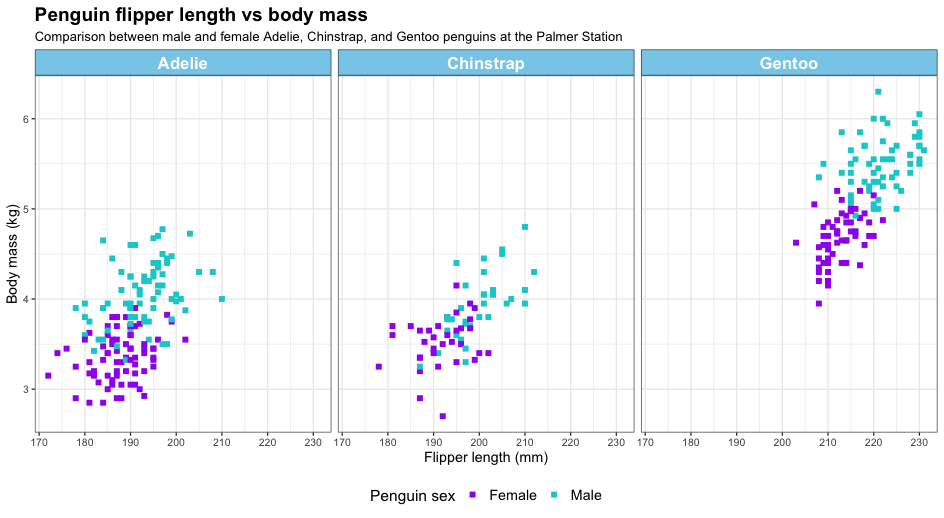
\includegraphics[width=1\linewidth]{images/04-Palmerspenguins} 

}

\caption{Example of plots created using `palmerspenguins`. Can you recreate this or improve on it?}\label{fig:palmerspenguins-plot}
\end{figure}

\begin{verbatim}
## Warning: Removed 11 rows containing missing values or values outside the scale range
## (`geom_point()`).
\end{verbatim}

\pandocbounded{\includegraphics[keepaspectratio]{_main_files/figure-latex/unnamed-chunk-126-1.pdf}}

\chapter{Hypothesis testing and regression modelling}\label{ch-5}

Before starting this chapter, make sure that you have the following R packages installed and loaded.

\begin{Shaded}
\begin{Highlighting}[]
\CommentTok{\#Install packages}
\NormalTok{utils}\SpecialCharTok{::}\FunctionTok{install.packages}\NormalTok{(}\StringTok{"tidyverse"}\NormalTok{)}
\NormalTok{utils}\SpecialCharTok{::}\FunctionTok{install.packages}\NormalTok{(}\StringTok{"gt"}\NormalTok{)}
\NormalTok{utils}\SpecialCharTok{::}\FunctionTok{install.packages}\NormalTok{(}\StringTok{"gtsummary"}\NormalTok{) }
\end{Highlighting}
\end{Shaded}

\begin{Shaded}
\begin{Highlighting}[]
\FunctionTok{library}\NormalTok{(tidyverse)}
\FunctionTok{library}\NormalTok{(gt)}
\FunctionTok{library}\NormalTok{(gtsummary)}

\FunctionTok{rm}\NormalTok{(}\AttributeTok{list=}\FunctionTok{ls}\NormalTok{()); }\FunctionTok{gc}\NormalTok{()}
\end{Highlighting}
\end{Shaded}

\begin{verbatim}
##           used  (Mb) gc trigger  (Mb) max used  (Mb)
## Ncells 2783975 148.7    4157530 222.1  4157530 222.1
## Vcells 4925432  37.6   10146329  77.5  8388608  64.0
\end{verbatim}

One primary aim of statistics is to make inferences, so that we can determine whether the association between the independent variable and the dependent variable (i.e., outcome) is true or could be due to chance. The independent variable may be an ``exposure'' (thought of as a potential cause), a ``predictor'' (which may or may not be causal), or a non-causal marker. Hypothesis testing is a common statistical method used to make such inferences.

In this chapter, we will use the data from Chapter \ref{ch-3}. To simplify things, we will only use the mean blood tests values, joined with the demographic table:

\begin{Shaded}
\begin{Highlighting}[]
\NormalTok{dat1 }\OtherTok{\textless{}{-}}\NormalTok{ utils}\SpecialCharTok{::}\FunctionTok{read.csv}\NormalTok{(}\StringTok{"data/03{-}diabetic\_demog.csv"}\NormalTok{)}
\NormalTok{dat2 }\OtherTok{\textless{}{-}}\NormalTok{ utils}\SpecialCharTok{::}\FunctionTok{read.csv}\NormalTok{(}\StringTok{"data/03{-}diabetic\_labs\_final\_with\_missing.csv"}\NormalTok{)}

\NormalTok{dat2 }\OtherTok{\textless{}{-}}\NormalTok{ dat2 }\SpecialCharTok{\%\textgreater{}\%} 
\NormalTok{  dplyr}\SpecialCharTok{::}\FunctionTok{summarise}\NormalTok{(}
    \FunctionTok{across}\NormalTok{(Chol}\SpecialCharTok{:}\NormalTok{BUN, }\SpecialCharTok{\textasciitilde{}}\FunctionTok{mean}\NormalTok{(.x, }\AttributeTok{na.rm=}\NormalTok{T)), }
    \AttributeTok{.by=}\NormalTok{id}
\NormalTok{  )}

\NormalTok{dat }\OtherTok{\textless{}{-}}\NormalTok{ dat1 }\SpecialCharTok{\%\textgreater{}\%} 
\NormalTok{  dplyr}\SpecialCharTok{::}\FunctionTok{inner\_join}\NormalTok{(dat2, }\AttributeTok{by=}\StringTok{\textquotesingle{}id\textquotesingle{}}\NormalTok{)}

\FunctionTok{head}\NormalTok{(dat)}
\end{Highlighting}
\end{Shaded}

\begin{verbatim}
##   id age Gender BMI SIMD     Chol       TG      HDL      LDL       Cr      BUN
## 1  5  28      M  26    4 4.450000 2.943333 2.286918 3.286918 71.90000 5.113333
## 2 14  12      M  23    4 5.645000 1.133333 2.650251 3.866918 58.03333 4.283333
## 3 16   9      F  30    2 4.336667 1.380000 2.576918 3.296918 68.50000 5.426667
## 4 25   9      M  28    3 4.800000 2.800000 1.350000 2.300000 43.50000 3.850000
## 5 29  13      M  36    4 4.835000 1.765000 1.285000 2.800000 52.45000 4.665000
## 6 46  12      F  20    2 5.670000 0.870000 3.180376 4.405377 65.85000 5.720000
\end{verbatim}

Note that the \texttt{across()} function has not been introduced in this course, but it can be a handy way to perform the same transformation across multiple variables. Please consult its \href{https://dplyr.tidyverse.org/reference/across.html}{help page} if you're interested.

\section{Overview of test choices}\label{overview-of-test-choices}

In statistics courses, you may have learned many different tests for various purposes. The following is a simplified summary of the tests that will be covered in this R course. Note that survival outcomes are taught in the Advanced Statistics course; how their analysis in R will be addressed in a later chapter.

{\def\LTcaptype{none} % do not increment counter
\begin{longtable}[]{@{}
  >{\raggedright\arraybackslash}p{(\linewidth - 10\tabcolsep) * \real{0.1379}}
  >{\centering\arraybackslash}p{(\linewidth - 10\tabcolsep) * \real{0.1724}}
  >{\centering\arraybackslash}p{(\linewidth - 10\tabcolsep) * \real{0.1724}}
  >{\centering\arraybackslash}p{(\linewidth - 10\tabcolsep) * \real{0.1724}}
  >{\centering\arraybackslash}p{(\linewidth - 10\tabcolsep) * \real{0.1724}}
  >{\centering\arraybackslash}p{(\linewidth - 10\tabcolsep) * \real{0.1724}}@{}}
\toprule\noalign{}
\begin{minipage}[b]{\linewidth}\raggedright
Predictors
\end{minipage} & \begin{minipage}[b]{\linewidth}\centering
Nil
\end{minipage} & \begin{minipage}[b]{\linewidth}\centering
Binary
\end{minipage} & \begin{minipage}[b]{\linewidth}\centering
Categorical
\end{minipage} & \begin{minipage}[b]{\linewidth}\centering
Numeric
\end{minipage} & \begin{minipage}[b]{\linewidth}\centering
Multiple
\end{minipage} \\
\midrule\noalign{}
\endhead
\bottomrule\noalign{}
\endlastfoot
\textbf{Numeric outcome} & One-sample t-test & Two-sample t-test & Analysis of variance & Correlation coefficients & General linear model \\
\textbf{Binary outcome} & One-sample proportion test & Two-sample proportion test & Chi-square test & Binary logistic model & Binary logistic model \\
\textbf{Count outcome} & Count regression & Count regression & Count regression & Count regression & Count regression \\
\textbf{Survival outcome} & Kaplan-Meier estimator & Log-rank test & Log-rank test & CoxPH model & CoxPH model \\
\end{longtable}
}

\section{Tests for one outcome variable}\label{tests-for-one-outcome-variable}

Tests for one outcome variable but no predictor variable usually compare the outcome against a fixed benchmark. An example of this is to see if the average \textbf{\hyperref[acronyms_BMI]{BMI}} of the sample is significantly different from 30, the threshold for obesity.

\subsection{One-sample t-test}\label{one-sample-t-test}

In R, all t-tests can be done with the \texttt{t.test()} function. In a one-sample t-test, we only need to specify the outcome variable, as well as the benchmark to test against (\textbf{\texttt{mu}}). Here, the benchmark is 30.

\begin{Shaded}
\begin{Highlighting}[]
\NormalTok{stats}\SpecialCharTok{::}\FunctionTok{t.test}\NormalTok{(dat}\SpecialCharTok{$}\NormalTok{BMI, }\AttributeTok{mu=}\DecValTok{30}\NormalTok{)}
\end{Highlighting}
\end{Shaded}

\begin{verbatim}
## 
##  One Sample t-test
## 
## data:  dat$BMI
## t = 2.8949, df = 188, p-value = 0.004242
## alternative hypothesis: true mean is not equal to 30
## 95 percent confidence interval:
##  30.45003 32.37536
## sample estimates:
## mean of x 
##   31.4127
\end{verbatim}

Here, the output in R shows that the mean \textbf{\hyperref[acronyms_BMI]{BMI}} of the sample was 31.4 (95\% \textbf{\hyperref[acronyms_CI]{confidence interval (CI)}}: 30.5 - 32.4). The p-value of the test was 0.004, indicating the mean \textbf{\hyperref[acronyms_BMI]{BMI}} was significantly different from 30.

\subsection{Wilcoxon signed rank test}\label{sec:WilcoxonSignedRankTest}

T-tests rely on the central limit theorem to work correctly. If the sample size is too small or the data are highly skewed, the results of those tests might not be reliable. The following shows how we can perform a Wilcoxon signed-rank test against a benchmark. The syntax is similar to that of a t-test: \texttt{wilcox.test()}.

\begin{Shaded}
\begin{Highlighting}[]
\NormalTok{stats}\SpecialCharTok{::}\FunctionTok{wilcox.test}\NormalTok{(dat}\SpecialCharTok{$}\NormalTok{BMI, }\AttributeTok{mu=}\DecValTok{30}\NormalTok{)}
\end{Highlighting}
\end{Shaded}

\begin{verbatim}
## 
##  Wilcoxon signed rank test with continuity correction
## 
## data:  dat$BMI
## V = 9004, p-value = 0.01081
## alternative hypothesis: true location is not equal to 30
\end{verbatim}

The R output does not provide any estimates, but just a p-value, which is also very close to zero, indicating the same conclusion as the one-sample t-test.

\subsection{One-sample proportion test}\label{sec:oneSamplePropTest}

Similarly, one might also be interested in determining whether the proportion in the sample (e.g., the proportion of individuals with obesity) differs from a specific benchmark (e.g.~10\%), which can be tested using the one-sample proportion test. The syntax for this is \texttt{prop.test()}. Both the number of diagnosed and the total number of observations need to be specified using \textbf{\texttt{x}} and \textbf{\texttt{n}}, respectively.

\begin{Shaded}
\begin{Highlighting}[]
\NormalTok{dat }\OtherTok{\textless{}{-}}\NormalTok{ dat }\SpecialCharTok{\%\textgreater{}\%}
\NormalTok{  dplyr}\SpecialCharTok{::}\FunctionTok{mutate}\NormalTok{(}\AttributeTok{obesity=}\FunctionTok{ifelse}\NormalTok{(BMI }\SpecialCharTok{\textgreater{}=} \DecValTok{30}\NormalTok{, }\DecValTok{1}\NormalTok{, }\DecValTok{0}\NormalTok{))}
\NormalTok{stats}\SpecialCharTok{::}\FunctionTok{prop.test}\NormalTok{(}\AttributeTok{x=}\FunctionTok{sum}\NormalTok{(dat}\SpecialCharTok{$}\NormalTok{obesity), }\AttributeTok{n=}\FunctionTok{length}\NormalTok{(dat}\SpecialCharTok{$}\NormalTok{obesity), }\AttributeTok{p=}\FloatTok{0.10}\NormalTok{)}
\end{Highlighting}
\end{Shaded}

\begin{verbatim}
## 
##  1-sample proportions test with continuity correction
## 
## data:  sum(dat$obesity) out of length(dat$obesity), null probability 0.1
## X-squared = 515.05, df = 1, p-value < 2.2e-16
## alternative hypothesis: true p is not equal to 0.1
## 95 percent confidence interval:
##  0.5240373 0.6676841
## sample estimates:
##         p 
## 0.5978836
\end{verbatim}

Here, the output in R showed that the proportion (95\% \textbf{\hyperref[acronyms_CI]{CI}}) of obesity was 59.8\% (52.4-66.8). The p-value of the test was \textless0.001, indicating the proportion of \textbf{\hyperref[acronyms_DM]{DM}} was significantly different from 10\%.

\section{Tests for one outcome variable and one exposure/predictor}\label{tests-for-one-outcome-variable-and-one-exposurepredictor}

\subsection{Independent two-sample t-test}\label{independent-two-sample-t-test}

Note that in the code sample below, instead of specifying \texttt{dat\$} before \textbf{\hyperref[acronyms_BMI]{BMI}} and Gender, the whole line of code was enclosed by a \textbf{\texttt{base::with(dat,\ ...)}} function. The \texttt{with()} function tells R to evaluate the \texttt{t.test()} function by finding the variables inside \texttt{dat}.

\begin{Shaded}
\begin{Highlighting}[]
\NormalTok{base}\SpecialCharTok{::}\FunctionTok{with}\NormalTok{(dat, stats}\SpecialCharTok{::}\FunctionTok{t.test}\NormalTok{(BMI }\SpecialCharTok{\textasciitilde{}}\NormalTok{ Gender))}
\end{Highlighting}
\end{Shaded}

\begin{verbatim}
## 
##  Welch Two Sample t-test
## 
## data:  BMI by Gender
## t = -0.85871, df = 180.49, p-value = 0.3916
## alternative hypothesis: true difference in means between group F and group M is not equal to 0
## 95 percent confidence interval:
##  -2.782425  1.095009
## sample estimates:
## mean in group F mean in group M 
##        30.96629        31.81000
\end{verbatim}

\subsection{Wilcoxon rank sum test}\label{wilcoxon-rank-sum-test}

When the sample size is too small (a common rule of thumb is n \textless{} 30) and/or the variable is highly skewed, the central limit theorem might not work well. In this scenario, using non-parametric tests, such as the Wilcoxon rank-sum test (\texttt{wilcox.test()}) could be an option.

\begin{Shaded}
\begin{Highlighting}[]
\NormalTok{base}\SpecialCharTok{::}\FunctionTok{with}\NormalTok{(dat, stats}\SpecialCharTok{::}\FunctionTok{wilcox.test}\NormalTok{(BMI }\SpecialCharTok{\textasciitilde{}}\NormalTok{ Gender))}
\end{Highlighting}
\end{Shaded}

\begin{verbatim}
## 
##  Wilcoxon rank sum test with continuity correction
## 
## data:  BMI by Gender
## W = 4106, p-value = 0.3594
## alternative hypothesis: true location shift is not equal to 0
\end{verbatim}

\subsection{Paired t-test}\label{paired-t-test}

The paired t-test is useful when a study has a matched design or when the data have repeated measures. To illustrate a paired t-test, we will use the data from Chapter \ref{ch-3}. The code below demonstrates how to convert long-format data into wide format, including total cholesterol.

\begin{Shaded}
\begin{Highlighting}[]
\NormalTok{dat2 }\OtherTok{\textless{}{-}}\NormalTok{ utils}\SpecialCharTok{::}\FunctionTok{read.csv}\NormalTok{(}\StringTok{"data/03{-}diabetic\_labs\_final\_with\_missing.csv"}\NormalTok{)   }
\NormalTok{dat2 }\OtherTok{\textless{}{-}}\NormalTok{ dat2 }\SpecialCharTok{\%\textgreater{}\%} 
\NormalTok{  dplyr}\SpecialCharTok{::}\FunctionTok{group\_by}\NormalTok{(id) }\SpecialCharTok{\%\textgreater{}\%}
\NormalTok{  dplyr}\SpecialCharTok{::}\FunctionTok{mutate}\NormalTok{(}\AttributeTok{t=}\DecValTok{1}\SpecialCharTok{:}\FunctionTok{n}\NormalTok{()) }\SpecialCharTok{\%\textgreater{}\%}
\NormalTok{  dplyr}\SpecialCharTok{::}\FunctionTok{ungroup}\NormalTok{() }\SpecialCharTok{\%\textgreater{}\%}
\NormalTok{  dplyr}\SpecialCharTok{::}\FunctionTok{select}\NormalTok{(id, t, Chol) }\SpecialCharTok{\%\textgreater{}\%}
\NormalTok{  tidyr}\SpecialCharTok{::}\FunctionTok{pivot\_wider}\NormalTok{(}\AttributeTok{id\_cols =}\NormalTok{ id, }\AttributeTok{names\_from =}\NormalTok{ t, }\AttributeTok{names\_prefix =} \StringTok{"Chol\_"}\NormalTok{, }
    \AttributeTok{values\_from =}\NormalTok{ Chol)}
\FunctionTok{head}\NormalTok{(dat2)}
\end{Highlighting}
\end{Shaded}

\begin{verbatim}
## # A tibble: 6 x 4
##      id Chol_1 Chol_2 Chol_3
##   <int>  <dbl>  <dbl>  <dbl>
## 1     5   4.9    3.6    4.85
## 2    14   6.49  NA      4.8 
## 3    16   3.3    4.31   5.4 
## 4    25   5      4.6   NA   
## 5    29   4.17   5.5   NA   
## 6    46   5.83   5.51  NA
\end{verbatim}

Can you deconstruct the code above and explain what it does in each step?

Once the wide-format data are ready, it is very straightforward to conduct a paired t-test. Put the two vectors in and specify \textbf{\texttt{paired=T}}:

\begin{Shaded}
\begin{Highlighting}[]
\NormalTok{base}\SpecialCharTok{::}\FunctionTok{with}\NormalTok{(dat2, stats}\SpecialCharTok{::}\FunctionTok{t.test}\NormalTok{(Chol\_1, Chol\_2, }\AttributeTok{paired=}\NormalTok{T))}
\end{Highlighting}
\end{Shaded}

\begin{verbatim}
## 
##  Paired t-test
## 
## data:  Chol_1 and Chol_2
## t = 0.68612, df = 187, p-value = 0.4935
## alternative hypothesis: true mean difference is not equal to 0
## 95 percent confidence interval:
##  -0.1328674  0.2745775
## sample estimates:
## mean difference 
##      0.07085507
\end{verbatim}

\subsection{Two-sample proportion test}\label{two-sample-proportion-test}

If the outcome variable is binary, we can perform the two-sample proportion test to examine the differences in proportion by a binary variable (i.e., gender). It is easiest to provide a 2x2 contingency table using the \texttt{table()} function.

\begin{Shaded}
\begin{Highlighting}[]
\NormalTok{base}\SpecialCharTok{::}\FunctionTok{with}\NormalTok{(dat, stats}\SpecialCharTok{::}\FunctionTok{prop.test}\NormalTok{(base}\SpecialCharTok{::}\FunctionTok{table}\NormalTok{(Gender, obesity)))}
\end{Highlighting}
\end{Shaded}

\begin{verbatim}
## 
##  2-sample test for equality of proportions with continuity correction
## 
## data:  base::table(Gender, obesity)
## X-squared = 0.64948, df = 1, p-value = 0.4203
## alternative hypothesis: two.sided
## 95 percent confidence interval:
##  -0.08234507  0.21874956
## sample estimates:
##    prop 1    prop 2 
## 0.4382022 0.3700000
\end{verbatim}

\subsection{Chi-square test of independence}\label{sec:chiSqrd}

When examining the association between two categorical variables, the Chi-square test of independence can be used. For illustrative purposes, we will create a new variable for \textbf{\hyperref[acronyms_BMI]{BMI}} categories.

\begin{Shaded}
\begin{Highlighting}[]
\NormalTok{dat }\OtherTok{\textless{}{-}}\NormalTok{ dat }\SpecialCharTok{\%\textgreater{}\%} 
\NormalTok{ dplyr}\SpecialCharTok{::}\FunctionTok{mutate}\NormalTok{(}\AttributeTok{BMI\_cat =}\NormalTok{ dplyr}\SpecialCharTok{::}\FunctionTok{case\_when}\NormalTok{(BMI }\SpecialCharTok{\textgreater{}=} \DecValTok{30} \SpecialCharTok{\textasciitilde{}} \DecValTok{2}\NormalTok{, }
\NormalTok{                            BMI }\SpecialCharTok{\textgreater{}=} \DecValTok{25} \SpecialCharTok{\textasciitilde{}} \DecValTok{1}\NormalTok{, }
\NormalTok{                            BMI }\SpecialCharTok{\textgreater{}=} \FloatTok{18.5} \SpecialCharTok{\textasciitilde{}} \DecValTok{0}\NormalTok{, }
\NormalTok{                            BMI }\SpecialCharTok{\textgreater{}=} \DecValTok{0} \SpecialCharTok{\textasciitilde{}} \SpecialCharTok{{-}}\DecValTok{1}\NormalTok{))}
\FunctionTok{head}\NormalTok{(dat)}
\end{Highlighting}
\end{Shaded}

\begin{verbatim}
##   id age Gender BMI SIMD     Chol       TG      HDL      LDL       Cr      BUN
## 1  5  28      M  26    4 4.450000 2.943333 2.286918 3.286918 71.90000 5.113333
## 2 14  12      M  23    4 5.645000 1.133333 2.650251 3.866918 58.03333 4.283333
## 3 16   9      F  30    2 4.336667 1.380000 2.576918 3.296918 68.50000 5.426667
## 4 25   9      M  28    3 4.800000 2.800000 1.350000 2.300000 43.50000 3.850000
## 5 29  13      M  36    4 4.835000 1.765000 1.285000 2.800000 52.45000 4.665000
## 6 46  12      F  20    2 5.670000 0.870000 3.180376 4.405377 65.85000 5.720000
##   obesity BMI_cat
## 1       0       1
## 2       0       0
## 3       1       2
## 4       0       1
## 5       1       2
## 6       0       0
\end{verbatim}

Can you use R to check the validity of the \textbf{\hyperref[acronyms_BMI]{BMI}} category variable? Hint: check descriptive statistics and/or distribution of \textbf{\hyperref[acronyms_BMI]{BMI}} by \textbf{\hyperref[acronyms_BMI]{BMI}} categories.

\begin{Shaded}
\begin{Highlighting}[]
\NormalTok{base}\SpecialCharTok{::}\FunctionTok{with}\NormalTok{(dat, stats}\SpecialCharTok{::}\FunctionTok{chisq.test}\NormalTok{(Gender, BMI\_cat))}
\end{Highlighting}
\end{Shaded}

\begin{verbatim}
## Warning in stats::chisq.test(Gender, BMI_cat): Chi-squared approximation may be
## incorrect
\end{verbatim}

\begin{verbatim}
## 
##  Pearson's Chi-squared test
## 
## data:  Gender and BMI_cat
## X-squared = 1.6114, df = 3, p-value = 0.6568
\end{verbatim}

Note that R threw a warning that the Chi-squared approximation may be incorrect due to lower cell counts.

\subsection{Fisher exact test}\label{sec:fisherExact}

Since the chi-square test was potentially violated, we can use the Fisher test, \texttt{fisher.test()}.

\begin{Shaded}
\begin{Highlighting}[]
\NormalTok{base}\SpecialCharTok{::}\FunctionTok{with}\NormalTok{(dat, stats}\SpecialCharTok{::}\FunctionTok{fisher.test}\NormalTok{(Gender, BMI\_cat))}
\end{Highlighting}
\end{Shaded}

\begin{verbatim}
## 
##  Fisher's Exact Test for Count Data
## 
## data:  Gender and BMI_cat
## p-value = 0.6525
## alternative hypothesis: two.sided
\end{verbatim}

Fisher's test can be computationally intensive. To overcome this, you can specify a larger workspace:

\begin{Shaded}
\begin{Highlighting}[]
\NormalTok{base}\SpecialCharTok{::}\FunctionTok{with}\NormalTok{(dat, stats}\SpecialCharTok{::}\FunctionTok{fisher.test}\NormalTok{(Gender, BMI\_cat, }\AttributeTok{workspace =} \FloatTok{1e8}\NormalTok{))}
\end{Highlighting}
\end{Shaded}

\begin{verbatim}
## 
##  Fisher's Exact Test for Count Data
## 
## data:  Gender and BMI_cat
## p-value = 0.6525
## alternative hypothesis: two.sided
\end{verbatim}

Or use simulation:

\begin{Shaded}
\begin{Highlighting}[]
\NormalTok{base}\SpecialCharTok{::}\FunctionTok{with}\NormalTok{(dat, stats}\SpecialCharTok{::}\FunctionTok{fisher.test}\NormalTok{(Gender, BMI\_cat, }\AttributeTok{simulate.p.value =}\NormalTok{ T))}
\end{Highlighting}
\end{Shaded}

\begin{verbatim}
## 
##  Fisher's Exact Test for Count Data with simulated p-value (based on
##  2000 replicates)
## 
## data:  Gender and BMI_cat
## p-value = 0.6507
## alternative hypothesis: two.sided
\end{verbatim}

\subsection{Correlation coefficient}\label{sec:pearson-Spearman}

Pearson's correlation coefficients can be calculated using \texttt{cor.test()}:

\begin{Shaded}
\begin{Highlighting}[]
\NormalTok{base}\SpecialCharTok{::}\FunctionTok{with}\NormalTok{(dat, stats}\SpecialCharTok{::}\FunctionTok{cor.test}\NormalTok{(BMI, Chol))}
\end{Highlighting}
\end{Shaded}

\begin{verbatim}
## 
##  Pearson's product-moment correlation
## 
## data:  BMI and Chol
## t = -1.8635, df = 187, p-value = 0.06396
## alternative hypothesis: true correlation is not equal to 0
## 95 percent confidence interval:
##  -0.272503911  0.007856303
## sample estimates:
##        cor 
## -0.1350254
\end{verbatim}

For ordinal variables, use Spearman's by including \textbf{\texttt{method\ =\ "spearman"}}.

Attempt the following:
1. Conduct a formal statistical test to check whether total cholesterol is statistically different by diagnosis of diabetes.
2. Create a binary variable to indicate high cholesterol (1 where \textbf{\hyperref[acronyms_Chol]{cholesterol (Chol)}} \textgreater= 5 or 0 where \textbf{\hyperref[acronyms_Chol]{Chol}} \textless{} 5). Conduct a test to examine if there is an association between high cholesterol and \textbf{\hyperref[acronyms_BMI]{BMI}} categories.
3. Is there a correlation between total cholesterol and \textbf{\hyperref[acronyms_LDL]{low-density lipoprotein (LDL)}}? Can you use a plot to illustrate and conduct a formal statistical test to confirm?

\section{\texorpdfstring{Using \texttt{gtsummary} for ``Table 1''}{Using gtsummary for ``Table 1''}}\label{using-gtsummary-for-table-1}

In R, we can use the \texttt{gtsummary} package to help us with publication-quality tables. Suppose we want to show the characteristics of our study sample by gender:

\begin{Shaded}
\begin{Highlighting}[]
\NormalTok{dat }\SpecialCharTok{\%\textgreater{}\%}
\NormalTok{  gtsummary}\SpecialCharTok{::}\FunctionTok{tbl\_summary}\NormalTok{(}\AttributeTok{by=}\NormalTok{Gender, }\AttributeTok{include=}\DecValTok{2}\SpecialCharTok{:}\DecValTok{10}\NormalTok{)}
\end{Highlighting}
\end{Shaded}

\begin{table}[t]
\fontsize{12.0pt}{14.0pt}\selectfont
\begin{tabular*}{\linewidth}{@{\extracolsep{\fill}}lcc}
\toprule
\textbf{Characteristic} & \textbf{F}  N = 89\textsuperscript{\textit{1}} & \textbf{M}  N = 100\textsuperscript{\textit{1}} \\ 
\midrule\addlinespace[2.5pt]
age & 16 (10, 35) & 15 (9, 28) \\ 
BMI & 30 (26, 36) & 31 (28, 36) \\ 
SIMD &  &  \\ 
    1 & 12 (13\%) & 19 (19\%) \\ 
    2 & 21 (24\%) & 19 (19\%) \\ 
    3 & 19 (21\%) & 17 (17\%) \\ 
    4 & 23 (26\%) & 26 (26\%) \\ 
    5 & 14 (16\%) & 19 (19\%) \\ 
Chol & 4.92 (4.57, 5.35) & 4.89 (4.57, 5.34) \\ 
TG & 2.09 (1.65, 2.65) & 2.10 (1.52, 2.65) \\ 
HDL & 1.51 (1.16, 2.59) & 2.04 (1.26, 2.64) \\ 
LDL & 3.19 (2.76, 3.68) & 3.13 (2.62, 3.66) \\ 
Cr & 68 (61, 77) & 70 (59, 78) \\ 
\bottomrule
\end{tabular*}
\begin{minipage}{\linewidth}
\vspace{.05em}
\textsuperscript{\textit{1}}Median (Q1, Q3); n (\%)\\
\end{minipage}
\end{table}

If we want to change it to mean and \textbf{\hyperref[acronyms_SD]{SD}}:

\begin{Shaded}
\begin{Highlighting}[]
\NormalTok{dat }\SpecialCharTok{\%\textgreater{}\%}
\NormalTok{  gtsummary}\SpecialCharTok{::}\FunctionTok{tbl\_summary}\NormalTok{(}\AttributeTok{by=}\NormalTok{Gender, }\AttributeTok{include=}\DecValTok{2}\SpecialCharTok{:}\DecValTok{10}\NormalTok{, }
              \AttributeTok{statistic =} \FunctionTok{list}\NormalTok{(}\FunctionTok{all\_continuous}\NormalTok{() }\SpecialCharTok{\textasciitilde{}} \StringTok{"\{mean\} (\{sd\})"}\NormalTok{))}
\end{Highlighting}
\end{Shaded}

\begin{table}[t]
\fontsize{12.0pt}{14.0pt}\selectfont
\begin{tabular*}{\linewidth}{@{\extracolsep{\fill}}lcc}
\toprule
\textbf{Characteristic} & \textbf{F}  N = 89\textsuperscript{\textit{1}} & \textbf{M}  N = 100\textsuperscript{\textit{1}} \\ 
\midrule\addlinespace[2.5pt]
age & 22 (16) & 20 (14) \\ 
BMI & 31 (7) & 32 (6) \\ 
SIMD &  &  \\ 
    1 & 12 (13\%) & 19 (19\%) \\ 
    2 & 21 (24\%) & 19 (19\%) \\ 
    3 & 19 (21\%) & 17 (17\%) \\ 
    4 & 23 (26\%) & 26 (26\%) \\ 
    5 & 14 (16\%) & 19 (19\%) \\ 
Chol & 4.97 (0.67) & 4.94 (0.56) \\ 
TG & 2.21 (0.84) & 2.13 (0.76) \\ 
HDL & 1.95 (0.93) & 2.02 (0.91) \\ 
LDL & 3.21 (0.76) & 3.12 (0.68) \\ 
Cr & 72 (41) & 71 (21) \\ 
\bottomrule
\end{tabular*}
\begin{minipage}{\linewidth}
\vspace{.05em}
\textsuperscript{\textit{1}}Mean (SD); n (\%)\\
\end{minipage}
\end{table}

To add p-values, use \texttt{add\_p()}:

\begin{Shaded}
\begin{Highlighting}[]
\NormalTok{dat }\SpecialCharTok{\%\textgreater{}\%}
\NormalTok{  gtsummary}\SpecialCharTok{::}\FunctionTok{tbl\_summary}\NormalTok{(}\AttributeTok{by=}\NormalTok{Gender, }\AttributeTok{include=}\DecValTok{2}\SpecialCharTok{:}\DecValTok{10}\NormalTok{, }
              \AttributeTok{statistic =} \FunctionTok{list}\NormalTok{(}\FunctionTok{all\_continuous}\NormalTok{() }\SpecialCharTok{\textasciitilde{}} \StringTok{"\{mean\} (\{sd\})"}\NormalTok{)) }\SpecialCharTok{\%\textgreater{}\%}
\NormalTok{  gtsummary}\SpecialCharTok{::}\FunctionTok{add\_p}\NormalTok{()}
\end{Highlighting}
\end{Shaded}

\begin{table}[t]
\fontsize{12.0pt}{14.0pt}\selectfont
\begin{tabular*}{\linewidth}{@{\extracolsep{\fill}}lccc}
\toprule
\textbf{Characteristic} & \textbf{F}  N = 89\textsuperscript{\textit{1}} & \textbf{M}  N = 100\textsuperscript{\textit{1}} & \textbf{p-value}\textsuperscript{\textit{2}} \\ 
\midrule\addlinespace[2.5pt]
age & 22 (16) & 20 (14) & 0.3 \\ 
BMI & 31 (7) & 32 (6) & 0.4 \\ 
SIMD &  &  & 0.7 \\ 
    1 & 12 (13\%) & 19 (19\%) &  \\ 
    2 & 21 (24\%) & 19 (19\%) &  \\ 
    3 & 19 (21\%) & 17 (17\%) &  \\ 
    4 & 23 (26\%) & 26 (26\%) &  \\ 
    5 & 14 (16\%) & 19 (19\%) &  \\ 
Chol & 4.97 (0.67) & 4.94 (0.56) & 0.8 \\ 
TG & 2.21 (0.84) & 2.13 (0.76) & 0.6 \\ 
HDL & 1.95 (0.93) & 2.02 (0.91) & 0.6 \\ 
LDL & 3.21 (0.76) & 3.12 (0.68) & 0.5 \\ 
Cr & 72 (41) & 71 (21) & 0.5 \\ 
\bottomrule
\end{tabular*}
\begin{minipage}{\linewidth}
\vspace{.05em}
\textsuperscript{\textit{1}}Mean (SD); n (\%)\\
\textsuperscript{\textit{2}}Wilcoxon rank sum test; Pearson's Chi-squared test\\
\end{minipage}
\end{table}

Can you create a characteristic table to display the demographic and biomarker values of the study sample overall, as well as by diabetes diagnosis? Please also add p-values for the differences by diabetes diagnosis.

\section{General linear models}\label{general-linear-models}

General linear models describe a family of regression models for numeric outcomes and can be modelled using the \texttt{lm()} function in R.

\subsection{Simple linear regression}\label{sec:simpleLinearRegression}

In R, regression models are most often specified using a ``formula'' notation containing a \textbf{\texttt{\textasciitilde{}}}. The left side is the outcome; the right side is the predictor.

\begin{Shaded}
\begin{Highlighting}[]
\NormalTok{mod }\OtherTok{\textless{}{-}}\NormalTok{ stats}\SpecialCharTok{::}\FunctionTok{lm}\NormalTok{(Chol }\SpecialCharTok{\textasciitilde{}}\NormalTok{ BMI, }\AttributeTok{data =}\NormalTok{ dat)}
\NormalTok{base}\SpecialCharTok{::}\FunctionTok{summary}\NormalTok{(mod)}
\end{Highlighting}
\end{Shaded}

\begin{verbatim}
## 
## Call:
## stats::lm(formula = Chol ~ BMI, data = dat)
## 
## Residuals:
##      Min       1Q   Median       3Q      Max 
## -1.62666 -0.35944 -0.04105  0.40239  1.74120 
## 
## Coefficients:
##              Estimate Std. Error t value Pr(>|t|)    
## (Intercept)  5.342058   0.212017  25.196   <2e-16 ***
## BMI         -0.012302   0.006601  -1.864    0.064 .  
## ---
## Signif. codes:  0 '***' 0.001 '**' 0.01 '*' 0.05 '.' 0.1 ' ' 1
## 
## Residual standard error: 0.6072 on 187 degrees of freedom
## Multiple R-squared:  0.01823,    Adjusted R-squared:  0.01298 
## F-statistic: 3.473 on 1 and 187 DF,  p-value: 0.06396
\end{verbatim}

\subsection{Multiple regression}\label{multiple-regression}

Multiple regression can be done by adding \textbf{\texttt{+\ variables}} on the right side of the formula.

\begin{Shaded}
\begin{Highlighting}[]
\NormalTok{mod }\OtherTok{\textless{}{-}}\NormalTok{ stats}\SpecialCharTok{::}\FunctionTok{lm}\NormalTok{(Chol }\SpecialCharTok{\textasciitilde{}}\NormalTok{ BMI }\SpecialCharTok{+}\NormalTok{ age }\SpecialCharTok{+}\NormalTok{ Gender, }\AttributeTok{data =}\NormalTok{ dat)}
\NormalTok{base}\SpecialCharTok{::}\FunctionTok{summary}\NormalTok{(mod)}
\end{Highlighting}
\end{Shaded}

\begin{verbatim}
## 
## Call:
## stats::lm(formula = Chol ~ BMI + age + Gender, data = dat)
## 
## Residuals:
##      Min       1Q   Median       3Q      Max 
## -1.70777 -0.35841 -0.03938  0.39706  1.84994 
## 
## Coefficients:
##              Estimate Std. Error t value Pr(>|t|)    
## (Intercept)  5.460372   0.226468  24.111   <2e-16 ***
## BMI         -0.012549   0.006611  -1.898   0.0592 .  
## age         -0.004555   0.002978  -1.530   0.1278    
## GenderM     -0.030336   0.088909  -0.341   0.7333    
## ---
## Signif. codes:  0 '***' 0.001 '**' 0.01 '*' 0.05 '.' 0.1 ' ' 1
## 
## Residual standard error: 0.6066 on 185 degrees of freedom
## Multiple R-squared:  0.03072,    Adjusted R-squared:  0.01501 
## F-statistic: 1.955 on 3 and 185 DF,  p-value: 0.1224
\end{verbatim}

\subsection{Analysis of variance}\label{sec:anova}

The \textbf{\hyperref[acronyms_ANOVA]{analysis of variance (ANOVA)}} model is a special case of the general linear model, used when the predictor is ordinal or categorical.

\begin{Shaded}
\begin{Highlighting}[]
\NormalTok{mod }\OtherTok{\textless{}{-}}\NormalTok{ stats}\SpecialCharTok{::}\FunctionTok{aov}\NormalTok{(Chol }\SpecialCharTok{\textasciitilde{}}\NormalTok{ BMI\_cat, }\AttributeTok{data =}\NormalTok{ dat)}
\NormalTok{base}\SpecialCharTok{::}\FunctionTok{summary}\NormalTok{(mod)}
\end{Highlighting}
\end{Shaded}

\begin{verbatim}
##              Df Sum Sq Mean Sq F value Pr(>F)  
## BMI_cat       1   1.65  1.6479   4.493 0.0354 *
## Residuals   187  68.59  0.3668                 
## ---
## Signif. codes:  0 '***' 0.001 '**' 0.01 '*' 0.05 '.' 0.1 ' ' 1
\end{verbatim}

\subsection{Diagnostics}\label{diagnostics}

In general linear models, diagnostics can be done easily by plotting the model object. We use \texttt{graphics::par(mfrow=c(2,\ 2))} to arrange plots in a 2x2 panel.

\begin{Shaded}
\begin{Highlighting}[]
\NormalTok{graphics}\SpecialCharTok{::}\FunctionTok{par}\NormalTok{(}\AttributeTok{mfrow=}\FunctionTok{c}\NormalTok{(}\DecValTok{2}\NormalTok{, }\DecValTok{2}\NormalTok{))}
\NormalTok{graphics}\SpecialCharTok{::}\FunctionTok{plot}\NormalTok{(mod)}
\end{Highlighting}
\end{Shaded}

\pandocbounded{\includegraphics[keepaspectratio]{_main_files/figure-latex/unnamed-chunk-149-1.pdf}}

\section{Generalised linear models}\label{generalised-linear-models}

The \hyperref[acronyms_GLM]{generalised linear model (GLM)} is a even more general version of the general linear model. But the main difference is that general linear model only handles numeric outcomes, while the \hyperref[acronyms_GLM]{GLM} handles other types of outcome data. Note that because both model classes have the same acronyms and it could be confusing which `GLM' people refer to. But in this ebook `GLM' refers to generalised linear model.

\subsection{Binary outcomes}\label{binary-outcomes}

Below is an example of a binary logistic regression using \texttt{family\ =\ "binomial"}.

\begin{Shaded}
\begin{Highlighting}[]
\NormalTok{dat }\OtherTok{\textless{}{-}}\NormalTok{ dat }\SpecialCharTok{\%\textgreater{}\%} 
\NormalTok{  dplyr}\SpecialCharTok{::}\FunctionTok{mutate}\NormalTok{(}\AttributeTok{High\_chol =}\NormalTok{ base}\SpecialCharTok{::}\FunctionTok{ifelse}\NormalTok{(Chol }\SpecialCharTok{\textgreater{}=} \DecValTok{5}\NormalTok{, }\DecValTok{1}\NormalTok{, }\DecValTok{0}\NormalTok{))}
\NormalTok{mod }\OtherTok{\textless{}{-}}\NormalTok{ stats}\SpecialCharTok{::}\FunctionTok{glm}\NormalTok{(High\_chol }\SpecialCharTok{\textasciitilde{}}\NormalTok{ BMI, }\AttributeTok{data =}\NormalTok{ dat, }\AttributeTok{family =} \StringTok{"binomial"}\NormalTok{)}
\NormalTok{base}\SpecialCharTok{::}\FunctionTok{summary}\NormalTok{(mod)}
\end{Highlighting}
\end{Shaded}

\begin{verbatim}
## 
## Call:
## stats::glm(formula = High_chol ~ BMI, family = "binomial", data = dat)
## 
## Coefficients:
##             Estimate Std. Error z value Pr(>|z|)   
## (Intercept)  1.63209    0.74039   2.204   0.0275 * 
## BMI         -0.06080    0.02338  -2.601   0.0093 **
## ---
## Signif. codes:  0 '***' 0.001 '**' 0.01 '*' 0.05 '.' 0.1 ' ' 1
## 
## (Dispersion parameter for binomial family taken to be 1)
## 
##     Null deviance: 258.69  on 188  degrees of freedom
## Residual deviance: 251.50  on 187  degrees of freedom
## AIC: 255.5
## 
## Number of Fisher Scoring iterations: 4
\end{verbatim}

To calculate Odds Ratios (\textbf{\hyperref[acronyms_OR]{odds ratio (OR)}}) and CIs manually:

\begin{Shaded}
\begin{Highlighting}[]
\NormalTok{base}\SpecialCharTok{::}\FunctionTok{data.frame}\NormalTok{(}\AttributeTok{OR =}\NormalTok{ base}\SpecialCharTok{::}\FunctionTok{exp}\NormalTok{(base}\SpecialCharTok{::}\FunctionTok{summary}\NormalTok{(mod)}\SpecialCharTok{$}\NormalTok{coef[}\DecValTok{2}\NormalTok{, }\DecValTok{1}\NormalTok{]), }
           \AttributeTok{LCI=}\NormalTok{base}\SpecialCharTok{::}\FunctionTok{exp}\NormalTok{(stats}\SpecialCharTok{::}\FunctionTok{confint}\NormalTok{(mod)[}\DecValTok{2}\NormalTok{, }\DecValTok{1}\NormalTok{]), }
           \AttributeTok{UCI=}\NormalTok{base}\SpecialCharTok{::}\FunctionTok{exp}\NormalTok{(stats}\SpecialCharTok{::}\FunctionTok{confint}\NormalTok{(mod)[}\DecValTok{2}\NormalTok{, }\DecValTok{2}\NormalTok{]), }
           \AttributeTok{p=}\NormalTok{base}\SpecialCharTok{::}\FunctionTok{summary}\NormalTok{(mod)}\SpecialCharTok{$}\NormalTok{coef[}\DecValTok{2}\NormalTok{, }\DecValTok{4}\NormalTok{])}
\end{Highlighting}
\end{Shaded}

\begin{verbatim}
## Waiting for profiling to be done...
## Waiting for profiling to be done...
\end{verbatim}

\begin{verbatim}
##          OR       LCI       UCI          p
## 1 0.9410078 0.8974717 0.9840495 0.00929689
\end{verbatim}

Can you deconstruct the code above and explain what each part does? Specifically why the indices \textbf{\texttt{{[}2,\ 1{]}}}, \textbf{\texttt{{[}2,\ 2{]}}}, \textbf{\texttt{{[}2,\ 4{]}}} were used?

Alternatively, use \texttt{gtsummary}:

\begin{Shaded}
\begin{Highlighting}[]
\NormalTok{mod }\SpecialCharTok{\%\textgreater{}\%}\NormalTok{ gtsummary}\SpecialCharTok{::}\FunctionTok{tbl\_regression}\NormalTok{(}\AttributeTok{exp =}\NormalTok{ T)}
\end{Highlighting}
\end{Shaded}

\begin{table}[t]
\fontsize{12.0pt}{14.0pt}\selectfont
\begin{tabular*}{\linewidth}{@{\extracolsep{\fill}}lccc}
\toprule
\textbf{Characteristic} & \textbf{OR} & \textbf{95\% CI} & \textbf{p-value} \\ 
\midrule\addlinespace[2.5pt]
BMI & 0.94 & 0.90, 0.98 & 0.009 \\ 
\bottomrule
\end{tabular*}
\begin{minipage}{\linewidth}
\vspace{.05em}
Abbreviations: CI = Confidence Interval, OR = Odds Ratio\\
\end{minipage}
\end{table}

\subsection{Count outcomes}\label{count-outcomes}

Poisson regression can be used for count outcomes using \texttt{family\ =\ "poisson"}.

\begin{Shaded}
\begin{Highlighting}[]
\NormalTok{dat }\OtherTok{\textless{}{-}}\NormalTok{ dat }\SpecialCharTok{\%\textgreater{}\%} 
\NormalTok{  dplyr}\SpecialCharTok{::}\FunctionTok{mutate}\NormalTok{(}
  \AttributeTok{n\_lipid\_rf =}\NormalTok{ (Chol }\SpecialCharTok{\textgreater{}=} \DecValTok{5}\NormalTok{) }\SpecialCharTok{+} 
             \FunctionTok{case\_when}\NormalTok{(}
\NormalTok{               Gender}\SpecialCharTok{==}\StringTok{\textquotesingle{}M\textquotesingle{}} \SpecialCharTok{\&}\NormalTok{ HDL }\SpecialCharTok{\textless{}} \DecValTok{1} \SpecialCharTok{\textasciitilde{}} \DecValTok{1}\NormalTok{, }
\NormalTok{               Gender}\SpecialCharTok{==}\StringTok{\textquotesingle{}F\textquotesingle{}} \SpecialCharTok{\&}\NormalTok{ HDL }\SpecialCharTok{\textless{}} \FloatTok{1.2} \SpecialCharTok{\textasciitilde{}} \DecValTok{1}\NormalTok{, }
               \AttributeTok{.default =} \DecValTok{0}\NormalTok{, }
\NormalTok{             ) }\SpecialCharTok{+} 
\NormalTok{             (TG }\SpecialCharTok{\textgreater{}=} \FloatTok{1.7}\NormalTok{) }
\NormalTok{  )}
\NormalTok{graphics}\SpecialCharTok{::}\FunctionTok{hist}\NormalTok{(dat}\SpecialCharTok{$}\NormalTok{n\_lipid\_rf)}
\end{Highlighting}
\end{Shaded}

\pandocbounded{\includegraphics[keepaspectratio]{_main_files/figure-latex/unnamed-chunk-153-1.pdf}}

\begin{Shaded}
\begin{Highlighting}[]
\NormalTok{mod }\OtherTok{\textless{}{-}}\NormalTok{ stats}\SpecialCharTok{::}\FunctionTok{glm}\NormalTok{(n\_lipid\_rf }\SpecialCharTok{\textasciitilde{}}\NormalTok{ age }\SpecialCharTok{+}\NormalTok{ Gender }\SpecialCharTok{+}\NormalTok{ BMI, }
    \AttributeTok{data =}\NormalTok{ dat, }\AttributeTok{family =} \StringTok{"poisson"}\NormalTok{)}
\NormalTok{mod }\SpecialCharTok{\%\textgreater{}\%}\NormalTok{ gtsummary}\SpecialCharTok{::}\FunctionTok{tbl\_regression}\NormalTok{(}\AttributeTok{exp =}\NormalTok{ T)}
\end{Highlighting}
\end{Shaded}

\begin{table}[t]
\fontsize{12.0pt}{14.0pt}\selectfont
\begin{tabular*}{\linewidth}{@{\extracolsep{\fill}}lccc}
\toprule
\textbf{Characteristic} & \textbf{IRR} & \textbf{95\% CI} & \textbf{p-value} \\ 
\midrule\addlinespace[2.5pt]
age & 1.00 & 0.99, 1.01 & 0.8 \\ 
Gender &  &  &  \\ 
    F & — & — &  \\ 
    M & 0.85 & 0.66, 1.09 & 0.2 \\ 
BMI & 0.98 & 0.96, 1.00 & 0.075 \\ 
\bottomrule
\end{tabular*}
\begin{minipage}{\linewidth}
\vspace{.05em}
Abbreviations: CI = Confidence Interval, IRR = Incidence Rate Ratio\\
\end{minipage}
\end{table}

Check for overdispersion using the \texttt{performance} package:

\begin{Shaded}
\begin{Highlighting}[]
\NormalTok{performance}\SpecialCharTok{::}\FunctionTok{check\_overdispersion}\NormalTok{(mod)}
\end{Highlighting}
\end{Shaded}

\begin{verbatim}
## # Overdispersion test
## 
##        dispersion ratio =   0.567
##   Pearson's Chi-Squared = 104.905
##                 p-value =       1
\end{verbatim}

\begin{verbatim}
## No overdispersion detected.
\end{verbatim}

If overdispersed, use Negative Binomial regression via the \texttt{MASS} package:

\begin{Shaded}
\begin{Highlighting}[]
\NormalTok{mod }\OtherTok{\textless{}{-}}\NormalTok{ MASS}\SpecialCharTok{::}\FunctionTok{glm.nb}\NormalTok{(n\_lipid\_rf }\SpecialCharTok{\textasciitilde{}}\NormalTok{ age }\SpecialCharTok{+}\NormalTok{ Gender }\SpecialCharTok{+}\NormalTok{ BMI, }\AttributeTok{data =}\NormalTok{ dat)}
\end{Highlighting}
\end{Shaded}

\begin{verbatim}
## Warning in theta.ml(Y, mu, sum(w), w, limit = control$maxit, trace =
## control$trace > : iteration limit reached
## Warning in theta.ml(Y, mu, sum(w), w, limit = control$maxit, trace =
## control$trace > : iteration limit reached
\end{verbatim}

\begin{Shaded}
\begin{Highlighting}[]
\NormalTok{mod }\SpecialCharTok{\%\textgreater{}\%}\NormalTok{ gtsummary}\SpecialCharTok{::}\FunctionTok{tbl\_regression}\NormalTok{(}\AttributeTok{exp=}\NormalTok{T)}
\end{Highlighting}
\end{Shaded}

\begin{table}[t]
\fontsize{12.0pt}{14.0pt}\selectfont
\begin{tabular*}{\linewidth}{@{\extracolsep{\fill}}lccc}
\toprule
\textbf{Characteristic} & \textbf{IRR} & \textbf{95\% CI} & \textbf{p-value} \\ 
\midrule\addlinespace[2.5pt]
age & 1.00 & 0.99, 1.01 & 0.8 \\ 
Gender &  &  &  \\ 
    F & — & — &  \\ 
    M & 0.85 & 0.66, 1.09 & 0.2 \\ 
BMI & 0.98 & 0.96, 1.00 & 0.075 \\ 
\bottomrule
\end{tabular*}
\begin{minipage}{\linewidth}
\vspace{.05em}
Abbreviations: CI = Confidence Interval, IRR = Incidence Rate Ratio\\
\end{minipage}
\end{table}

\subsection{Sandwich estimator}\label{sandwich-estimator}

The sandwich estimator provides robust standard errors.

\begin{Shaded}
\begin{Highlighting}[]
\NormalTok{mod }\OtherTok{\textless{}{-}}\NormalTok{ stats}\SpecialCharTok{::}\FunctionTok{glm}\NormalTok{(n\_lipid\_rf }\SpecialCharTok{\textasciitilde{}}\NormalTok{ age }\SpecialCharTok{+}\NormalTok{ Gender }\SpecialCharTok{+}\NormalTok{ BMI, }\AttributeTok{data =}\NormalTok{ dat, }\AttributeTok{family =} \StringTok{"poisson"}\NormalTok{)}
\NormalTok{lmtest}\SpecialCharTok{::}\FunctionTok{coeftest}\NormalTok{(mod, }\AttributeTok{vcov =}\NormalTok{ sandwich}\SpecialCharTok{::}\NormalTok{sandwich)}
\end{Highlighting}
\end{Shaded}

\begin{verbatim}
## 
## z test of coefficients:
## 
##               Estimate Std. Error z value  Pr(>|z|)    
## (Intercept)  0.9098045  0.2337570  3.8921 9.938e-05 ***
## age         -0.0013351  0.0031579 -0.4228   0.67247    
## GenderM     -0.1608495  0.0941015 -1.7093   0.08739 .  
## BMI         -0.0171825  0.0071394 -2.4067   0.01610 *  
## ---
## Signif. codes:  0 '***' 0.001 '**' 0.01 '*' 0.05 '.' 0.1 ' ' 1
\end{verbatim}

\begin{enumerate}
\def\labelenumi{\arabic{enumi}.}
\tightlist
\item
  Can you test the association between total cholesterol (exposure) and diabetes diagnosis (outcome), adjusting for age and gender?
\item
  Create a new count variable on the number of metabolic risk factors: \textbf{\hyperref[acronyms_BMI]{BMI}} \textgreater= 30; total cholesterol \textgreater= 5; diabetes=1. Is there an association between age and gender with the number of metabolic risk factors? Please use an appropriate count regression to examine this.
\end{enumerate}

\section{Summary}\label{summary}

In this chapter, you have learnt to perform common statistical tests and regression models in R. The coding of these is generally straightforward, but the proper use and interpretation of them will require subject, epidemiological, and statistical knowledge.

\chapter{Advanced Topics in Regression}\label{ch-6}

Chapter \ref{ch-5} introduced how to fit an \textbf{\hyperref[acronyms_GLM]{GLM}} for outcomes of different data types. However, there is still one common type of outcome that cannot be handled using \textbf{\hyperref[acronyms_GLM]{GLM}}: \textbf{survival outcome}. Survival outcome can be thought of an extension of a binary outcome. But instead of just a yes/no for a disease, it has two pieces of information:

\begin{enumerate}
\def\labelenumi{\arabic{enumi}.}
\tightlist
\item
  The length of follow-up (thus the data have to be generated from a study design with some temporality);
\item
  Whether the individual had the outcome by the end of follow-up: Yes (the individual had the event {[}e.g.~disease{]}); No (the individual had not had the event, a.k.a \textbf{censored}).
\end{enumerate}

Because of this survival outcome is also sometimes called \textbf{time-to-event}.

There are usually three ways where the follow-up end:

\begin{enumerate}
\def\labelenumi{\arabic{enumi}.}
\tightlist
\item
  End of observation: There is no more information about the presence of the event after that. This is the most common way of ending a follow-up.
\item
  Observation of an event: In majority of scenarios, only the incident (i.e.~first) event was of interest, and thus follow-up would end at the incident event, even though the actual observation could be longer.
\item
  Occurrence of a \textbf{competing event}: Briefly, a competing event is one that would inhibit the observation of the main event of interest. A common competing event is death from other causes. For example, if one is interested in the incidence of heart diseases, dying from cancer is a competing event. Handling competing event is actually a very complex topic. In simplest term, if one is only interested in the \textbf{relative risk}, they can look at cause-specific \hyperref[acronyms_HR]{hazard ratio (HR)}, where a competing event will end the follow-up. Please note that this approach, however, will provide a biased estimate for \textbf{absolute risk} (e.g.~cumulative hazard) \citep{lau2009competing}. There is another method to handle competing event (`Fine and Grey subdistribution model'), but is outside the scope of this course.
\end{enumerate}

\begin{Shaded}
\begin{Highlighting}[]
\FunctionTok{library}\NormalTok{(tidyverse)}
\FunctionTok{library}\NormalTok{(gtsummary)}
\FunctionTok{library}\NormalTok{(interactionR)}
\FunctionTok{library}\NormalTok{(car)}
\FunctionTok{library}\NormalTok{(mfp2)}
\FunctionTok{library}\NormalTok{(mgcv)}
\FunctionTok{library}\NormalTok{(survival)}
\FunctionTok{library}\NormalTok{(haven)}
\end{Highlighting}
\end{Shaded}

\begin{Shaded}
\begin{Highlighting}[]
\CommentTok{\# Import datasets}
\NormalTok{alertrct }\OtherTok{\textless{}{-}}\NormalTok{ haven}\SpecialCharTok{::}\FunctionTok{read\_dta}\NormalTok{(}\StringTok{\textquotesingle{}data/06{-}alert\_rct.dta\textquotesingle{}}\NormalTok{)}
\NormalTok{usoc }\OtherTok{\textless{}{-}}\NormalTok{ readr}\SpecialCharTok{::}\FunctionTok{read\_csv}\NormalTok{(}\StringTok{\textquotesingle{}data/06{-}understanding\_soc.csv\textquotesingle{}}\NormalTok{) }\SpecialCharTok{\%\textgreater{}\%} 
  \FunctionTok{mutate}\NormalTok{(}
    \AttributeTok{obesity=}\FunctionTok{if\_else}\NormalTok{(bmi }\SpecialCharTok{\textgreater{}=} \DecValTok{30}\NormalTok{, }\DecValTok{1}\NormalTok{, }\DecValTok{0}\NormalTok{), }
    \AttributeTok{bmi\_factor=}\FunctionTok{case\_when}\NormalTok{(}
\NormalTok{      bmi }\SpecialCharTok{\textless{}=} \FloatTok{18.5} \SpecialCharTok{\textasciitilde{}} \StringTok{\textquotesingle{}Underweight\textquotesingle{}}\NormalTok{, }
\NormalTok{      bmi }\SpecialCharTok{\textless{}=} \DecValTok{25} \SpecialCharTok{\textasciitilde{}} \StringTok{\textquotesingle{}Normal weight\textquotesingle{}}\NormalTok{, }
\NormalTok{      bmi }\SpecialCharTok{\textless{}=} \DecValTok{30} \SpecialCharTok{\textasciitilde{}} \StringTok{\textquotesingle{}Overweight\textquotesingle{}}\NormalTok{, }
\NormalTok{      bmi }\SpecialCharTok{\textless{}=} \DecValTok{999} \SpecialCharTok{\textasciitilde{}} \StringTok{\textquotesingle{}Obesity\textquotesingle{}}\NormalTok{, }
\NormalTok{    ) }\SpecialCharTok{\%\textgreater{}\%} 
      \FunctionTok{factor}\NormalTok{() }\SpecialCharTok{\%\textgreater{}\%} 
      \FunctionTok{relevel}\NormalTok{(}\StringTok{\textquotesingle{}Normal weight\textquotesingle{}}\NormalTok{)}
\NormalTok{  )}
\end{Highlighting}
\end{Shaded}

\begin{verbatim}
## Rows: 11447 Columns: 10
## -- Column specification --------------------------------------------------------
## Delimiter: ","
## chr (2): sex, income
## dbl (8): age, bmi, pw1, mw1, pw5, mw5, pw9, mw9
## 
## i Use `spec()` to retrieve the full column specification for this data.
## i Specify the column types or set `show_col_types = FALSE` to quiet this message.
\end{verbatim}

\section{Survival Analysis}\label{survival-analysis}

Survival analysis specifically deals with time-to-event data. This is unique because it tracks both the duration of follow-up and the presence of the event at the end (disease/death).

\subsection{Kaplan-Meier Estimator}\label{kaplan-meier-estimator}

The \hyperref[acronyms_KM]{Kaplan-Meier estimator (KM)} is a non-parametric method to estimate the survival function, i.e.~how survival (or, disease-free, for disease outcomes) probability varies over time.

The code below shows the simplest form of \hyperref[acronyms_KM]{KM} - estimating the \hyperref[acronyms_MACE]{major adverse cardiovascular event (MACE)}-free probability for the all participants in the \emph{Alert RCT}. Note that We use \texttt{Surv(time,\ event)} to create a survival object in R that combines follow-up time and event status. The \texttt{\textasciitilde{}\ 1} indicates we are interested in the overall survival function for the entire sample.

Note that when calling the km1 object, it showed the data has 1000 participants with 109 \hyperref[acronyms_MACE]{MACE}. However, the median and corresponding \hyperref[acronyms_CI]{CI} were both \hyperref[acronyms_NA]{NA}. That is because to calculate median survival from this non-parametric method, at least 50\% of the participants have to had developed the event. There are parametric models that could be used to extraplote beyond the observation, even though those usually would be regarded very reliable.

Calling \texttt{summary(km1,\ times=5)} asked R to produce the 5-year survival probability, which was 0.9.

\begin{Shaded}
\begin{Highlighting}[]
\FunctionTok{library}\NormalTok{(survival)}
\CommentTok{\# Produce survival function }
\NormalTok{km1 }\OtherTok{\textless{}{-}} \FunctionTok{survfit}\NormalTok{(}\FunctionTok{Surv}\NormalTok{(mace\_t, mace\_i) }\SpecialCharTok{\textasciitilde{}} \DecValTok{1}\NormalTok{, }\AttributeTok{data=}\NormalTok{alertrct)}
\NormalTok{km1}
\end{Highlighting}
\end{Shaded}

\begin{verbatim}
## Call: survfit(formula = Surv(mace_t, mace_i) ~ 1, data = alertrct)
## 
##         n events median 0.95LCL 0.95UCL
## [1,] 1000    109     NA      NA      NA
\end{verbatim}

\begin{Shaded}
\begin{Highlighting}[]
\FunctionTok{summary}\NormalTok{(km1, }\AttributeTok{times=}\DecValTok{5}\NormalTok{)}
\end{Highlighting}
\end{Shaded}

\begin{verbatim}
## Call: survfit(formula = Surv(mace_t, mace_i) ~ 1, data = alertrct)
## 
##  time n.risk n.event survival std.err lower 95% CI upper 95% CI
##     5    775      95      0.9 0.00973        0.881        0.919
\end{verbatim}

Instead of the table, one can also visualise the \hyperref[acronyms_KM]{KM}, a Kaplan-Meier curve using the following command.

\begin{Shaded}
\begin{Highlighting}[]
\CommentTok{\# Plot survival function }
\FunctionTok{plot}\NormalTok{(km1, }\AttributeTok{main=}\StringTok{"Kaplan{-}Meier Curve"}\NormalTok{, }\AttributeTok{xlab=}\StringTok{"Time"}\NormalTok{, }\AttributeTok{ylab=}\StringTok{"Survival"}\NormalTok{)}
\end{Highlighting}
\end{Shaded}

\pandocbounded{\includegraphics[keepaspectratio]{_main_files/figure-latex/plot-km-1.pdf}}

The plot showed that the longest follow-up was just over 6 years (as shown in the x-axis), and that by the end of the study there were still over 80\% of the participants to be disease-free.

What do you think \texttt{summary(km1,\ times=10)} will show?

\subsection{Log-rank Test}\label{log-rank-test}

\hyperref[acronyms_KM]{KM} is just an estimator but it could also be a basis to conduct simple comparison, e.g.~by subgroup. This is specifically done via the \textbf{log-rank test}. The example below examined if the disease-free survival were different by randomised group (fluvastatin vs.~placebo).

\begin{Shaded}
\begin{Highlighting}[]
\CommentTok{\# Standard log{-}rank test (rho=0)}
\NormalTok{km2 }\OtherTok{\textless{}{-}} \FunctionTok{survdiff}\NormalTok{(}\FunctionTok{Surv}\NormalTok{(mace\_t, mace\_i) }\SpecialCharTok{\textasciitilde{}}\NormalTok{ randgrp, }\AttributeTok{data=}\NormalTok{alertrct, }\AttributeTok{rho=}\DecValTok{0}\NormalTok{)}
\NormalTok{km2}
\end{Highlighting}
\end{Shaded}

\begin{verbatim}
## Call:
## survdiff(formula = Surv(mace_t, mace_i) ~ randgrp, data = alertrct, 
##     rho = 0)
## 
##             N Observed Expected (O-E)^2/E (O-E)^2/V
## randgrp=0 506       60     55.1     0.437     0.884
## randgrp=1 494       49     53.9     0.447     0.884
## 
##  Chisq= 0.9  on 1 degrees of freedom, p= 0.3
\end{verbatim}

The test p-value is 0.30, above the usual cut-off of statistical significance. But this could very well be due to lower statistical power than actually no difference. Note that in survival analysis, the number of events is the main driver of power.

Do you know why \texttt{rho=0} is specified in the code above?

Can you investigate by running \texttt{?survfit}?

You can also plot the survival curves or, alternatively, Nelson-Aalan estimator for cumulative hazard by subgroups. Note the differences in arguments in the two plotting functions below. The \texttt{conf.int} indicates whether the 95\% \hyperref[acronyms_CI]{CI} are to be plotted. In the Nelson-Aalan plot because \hyperref[acronyms_CI]{CI} were plotted, the syntax also included \texttt{lty=c(1,\ 2,\ 2,\ 1,\ 2,\ 2)} to ask R to use dashed lines for the \hyperref[acronyms_CI]{CI}. The \texttt{fun=\textquotesingle{}cumhaz\textquotesingle{}} asks R to specifically to plot the cumulative hazard. Without that, the default would be the plot the \hyperref[acronyms_KM]{KM} estimator for survival.

\begin{Shaded}
\begin{Highlighting}[]
\NormalTok{km2 }\OtherTok{\textless{}{-}} \FunctionTok{survfit}\NormalTok{(}\FunctionTok{Surv}\NormalTok{(mace\_t, mace\_i) }\SpecialCharTok{\textasciitilde{}}\NormalTok{ randgrp, }\AttributeTok{data=}\NormalTok{alertrct)}
\FunctionTok{plot}\NormalTok{(km2, }\AttributeTok{conf.int =} \ConstantTok{FALSE}\NormalTok{, }\AttributeTok{ylab=}\StringTok{"Prob. of survival"}\NormalTok{, }\AttributeTok{xlab=}\StringTok{"Time in years"}\NormalTok{, }
     \AttributeTok{col=}\FunctionTok{c}\NormalTok{(}\StringTok{\textquotesingle{}red\textquotesingle{}}\NormalTok{, }\StringTok{\textquotesingle{}blue\textquotesingle{}}\NormalTok{))}
\FunctionTok{legend}\NormalTok{(}\DecValTok{0}\NormalTok{, }\FloatTok{0.2}\NormalTok{, }\AttributeTok{legend=}\FunctionTok{c}\NormalTok{(}\StringTok{"Placebo"}\NormalTok{, }\StringTok{"Fluvastatin"}\NormalTok{), }\AttributeTok{col=}\FunctionTok{c}\NormalTok{(}\StringTok{"red"}\NormalTok{, }\StringTok{"blue"}\NormalTok{), }
       \AttributeTok{lty=}\DecValTok{1}\NormalTok{, }\AttributeTok{cex=}\FloatTok{0.8}\NormalTok{)}
\end{Highlighting}
\end{Shaded}

\pandocbounded{\includegraphics[keepaspectratio]{_main_files/figure-latex/plot-km-groups-1.pdf}}

\begin{Shaded}
\begin{Highlighting}[]
\FunctionTok{plot}\NormalTok{(km2, }\AttributeTok{conf.int =} \ConstantTok{TRUE}\NormalTok{, }\AttributeTok{ylab=}\StringTok{"Cumulative hazard"}\NormalTok{, }\AttributeTok{xlab=}\StringTok{"Time in years"}\NormalTok{, }
     \AttributeTok{col=}\FunctionTok{c}\NormalTok{(}\StringTok{\textquotesingle{}red\textquotesingle{}}\NormalTok{, }\StringTok{\textquotesingle{}blue\textquotesingle{}}\NormalTok{), }\AttributeTok{lty=}\FunctionTok{c}\NormalTok{(}\DecValTok{1}\NormalTok{, }\DecValTok{2}\NormalTok{, }\DecValTok{2}\NormalTok{, }\DecValTok{1}\NormalTok{, }\DecValTok{2}\NormalTok{, }\DecValTok{2}\NormalTok{), }\AttributeTok{fun=}\StringTok{"cumhaz"}\NormalTok{)}
\FunctionTok{legend}\NormalTok{(}\DecValTok{0}\NormalTok{, }\FloatTok{0.2}\NormalTok{, }\AttributeTok{legend=}\FunctionTok{c}\NormalTok{(}\StringTok{"Placebo"}\NormalTok{, }\StringTok{"Fluvastatin"}\NormalTok{), }\AttributeTok{col=}\FunctionTok{c}\NormalTok{(}\StringTok{"red"}\NormalTok{, }\StringTok{"blue"}\NormalTok{), }
       \AttributeTok{lty=}\DecValTok{1}\NormalTok{, }\AttributeTok{cex=}\FloatTok{0.8}\NormalTok{)}
\end{Highlighting}
\end{Shaded}

\pandocbounded{\includegraphics[keepaspectratio]{_main_files/figure-latex/plot-km-groups-2.pdf}}

Note that hazard is very similar to incidence rate, so cumulative hazard can be thought of as the cumulative incidence rate. It is not equal to the probability of having the disease. It is actually similar to the \textbf{cumulative probability} of having the disease, and can be greater than 1 (probabilities are bounded by 0 and 1).

\subsection{Cox proportional hazard model}\label{cox-proportional-hazard-model}

The log-rank test can be thought of as the t-test for survival variables in that they shared the same limitations: not being able to quantify the difference, no inherent way to accommodate numeric predictor/exposure, and the lack of ability to adjust for covariates. For numeric, binary, and count outcomes, the \hyperref[acronyms_GLM]{GLM} provides a solution to these two limitations. Similarly, the \hyperref[acronyms_Coxux20PH]{Cox proportional hazards (Cox PH)} model provides a solution for survival data.

\hyperref[acronyms_Coxux20PH]{Cox PH} model (a.k.a. Cox model or Cox regression) is semi-parametric in that it doesn't assumes the underlying survival / hazard function of the survival outcome (non-parametric part). However, it does assumes how the relative hazard varies by the exposure / predictors (the parametric part).

Below are examples to examine the assocation of Fluvastatin (compared with placebo) with \hyperref[acronyms_MACE]{MACE} in two adjustment models.

\begin{Shaded}
\begin{Highlighting}[]
\NormalTok{cm1 }\OtherTok{\textless{}{-}} \FunctionTok{coxph}\NormalTok{(}\FunctionTok{Surv}\NormalTok{(mace\_t, mace\_i) }\SpecialCharTok{\textasciitilde{}}\NormalTok{ randgrp, }\AttributeTok{data=}\NormalTok{alertrct)}
\FunctionTok{summary}\NormalTok{(cm1)}
\end{Highlighting}
\end{Shaded}

\begin{verbatim}
## Call:
## coxph(formula = Surv(mace_t, mace_i) ~ randgrp, data = alertrct)
## 
##   n= 1000, number of events= 109 
## 
##            coef exp(coef) se(coef)      z Pr(>|z|)
## randgrp -0.1809    0.8345   0.1926 -0.939    0.348
## 
##         exp(coef) exp(-coef) lower .95 upper .95
## randgrp    0.8345      1.198    0.5721     1.217
## 
## Concordance= 0.514  (se = 0.024 )
## Likelihood ratio test= 0.89  on 1 df,   p=0.3
## Wald test            = 0.88  on 1 df,   p=0.3
## Score (logrank) test = 0.88  on 1 df,   p=0.3
\end{verbatim}

\begin{Shaded}
\begin{Highlighting}[]
\NormalTok{cm2 }\OtherTok{\textless{}{-}} \FunctionTok{coxph}\NormalTok{(}\FunctionTok{Surv}\NormalTok{(mace\_t, mace\_i) }\SpecialCharTok{\textasciitilde{}}\NormalTok{ randgrp }\SpecialCharTok{+}\NormalTok{ age }\SpecialCharTok{+}\NormalTok{ female, }\AttributeTok{data=}\NormalTok{alertrct)}
\FunctionTok{summary}\NormalTok{(cm2)}
\end{Highlighting}
\end{Shaded}

\begin{verbatim}
## Call:
## coxph(formula = Surv(mace_t, mace_i) ~ randgrp + age + female, 
##     data = alertrct)
## 
##   n= 1000, number of events= 109 
## 
##              coef exp(coef)  se(coef)      z Pr(>|z|)    
## randgrp -0.172099  0.841896  0.192871 -0.892    0.372    
## age      0.042483  1.043398  0.009388  4.525 6.03e-06 ***
## female  -0.171887  0.842075  0.207171 -0.830    0.407    
## ---
## Signif. codes:  0 '***' 0.001 '**' 0.01 '*' 0.05 '.' 0.1 ' ' 1
## 
##         exp(coef) exp(-coef) lower .95 upper .95
## randgrp    0.8419     1.1878    0.5769     1.229
## age        1.0434     0.9584    1.0244     1.063
## female     0.8421     1.1875    0.5611     1.264
## 
## Concordance= 0.62  (se = 0.029 )
## Likelihood ratio test= 22.29  on 3 df,   p=6e-05
## Wald test            = 21.82  on 3 df,   p=7e-05
## Score (logrank) test = 22.34  on 3 df,   p=6e-05
\end{verbatim}

The \hyperref[acronyms_HR]{HR} shown in the column of \texttt{exp(coef)} indicated Fluvastatin was associated with 16\% lower hazard of \hyperref[acronyms_MACE]{MACE}, even though the difference is not statistically significant. Also note that age, after adjusted for sex and Fluvastatin, was associated with \hyperref[acronyms_MACE]{MACE}, with an \hyperref[acronyms_HR]{HR} (95\% \hyperref[acronyms_CI]{CI}) of 1.04 (1.02-1.06). This suggests that each year of age was associated with 4\% high hazard in MACE.

Alternatively, you can also use the \texttt{gtsummary::tbl\_regression()} function to display the results from a Cox model:

\begin{Shaded}
\begin{Highlighting}[]
\FunctionTok{tbl\_merge}\NormalTok{(}\FunctionTok{list}\NormalTok{(}\FunctionTok{tbl\_regression}\NormalTok{(cm1, }\AttributeTok{exponentiate =}\NormalTok{ T), }
               \FunctionTok{tbl\_regression}\NormalTok{(cm2, }\AttributeTok{exponentiate =}\NormalTok{ T)), }
          \AttributeTok{tab\_spanner =} \FunctionTok{c}\NormalTok{(}\StringTok{\textquotesingle{}Unadjusted\textquotesingle{}}\NormalTok{, }\StringTok{\textquotesingle{}Age and sex adjusted\textquotesingle{}}\NormalTok{))}
\end{Highlighting}
\end{Shaded}

\begin{verbatim}
## The number rows in the tables to be merged do not match, which may result in
## rows appearing out of order.
## i See `tbl_merge()` (`?gtsummary::tbl_merge()`) help file for details. Use
##   `quiet=TRUE` to silence message.
\end{verbatim}

\begin{table}[t]
\fontsize{12.0pt}{14.0pt}\selectfont
\begin{tabular*}{\linewidth}{@{\extracolsep{\fill}}lcccccc}
\toprule
 & \multicolumn{3}{c}{{Unadjusted}} & \multicolumn{3}{c}{{Age and sex adjusted}} \\ 
\cmidrule(lr){2-4} \cmidrule(lr){5-7}
\textbf{Characteristic} & \textbf{HR} & \textbf{95\% CI} & \textbf{p-value} & \textbf{HR} & \textbf{95\% CI} & \textbf{p-value} \\ 
\midrule\addlinespace[2.5pt]
randomised group & 0.83 & 0.57, 1.22 & 0.3 & 0.84 & 0.58, 1.23 & 0.4 \\ 
age of patient &  &  &  & 1.04 & 1.02, 1.06 & <0.001 \\ 
sex &  &  &  & 0.84 & 0.56, 1.26 & 0.4 \\ 
\bottomrule
\end{tabular*}
\begin{minipage}{\linewidth}
\vspace{.05em}
Abbreviations: CI = Confidence Interval, HR = Hazard Ratio\\
\end{minipage}
\end{table}

\subsubsection{Proportional hazard assumption}\label{proportional-hazard-assumption}

One of the main assumption behind Cox model is the proportional hazard assumption. The proportional hazards assumption requires that the \hyperref[acronyms_HR]{HR} remains constant over the entire follow-up.

For instance, if the placebo group is twice as likely to experience MACE \textbf{only} at year 6 (something supported by the \hyperref[acronyms_KM]{KM} plot, albeit with \hyperref[acronyms_CI]{CI} overlaps), the assumption is violated.

To formally examine this assumption, one can look at the Schoenfeld residuals with the syntax below.

\begin{Shaded}
\begin{Highlighting}[]
\FunctionTok{par}\NormalTok{(}\AttributeTok{mfrow=}\FunctionTok{c}\NormalTok{(}\DecValTok{1}\NormalTok{, }\DecValTok{3}\NormalTok{))}
\FunctionTok{plot}\NormalTok{(}\FunctionTok{cox.zph}\NormalTok{(cm2))}
\end{Highlighting}
\end{Shaded}

\pandocbounded{\includegraphics[keepaspectratio]{_main_files/figure-latex/schoenfeld-1.pdf}}

\begin{Shaded}
\begin{Highlighting}[]
\FunctionTok{cox.zph}\NormalTok{(cm2)}
\end{Highlighting}
\end{Shaded}

\begin{verbatim}
##         chisq df    p
## randgrp 1.297  1 0.25
## age     0.201  1 0.65
## female  0.164  1 0.69
## GLOBAL  1.639  3 0.65
\end{verbatim}

The first two lines plot the Schoenfeld residual for each included exposure/predictor in a 1x3 (1 row; 3 columns) layout. The third line calculate the p-values of a time-varying \hyperref[acronyms_HR]{HR} (i.e.~HR varies over time). However even though the p-value for \texttt{randgrp} is 0.25, the plot did show a tendency for HR to be lower towards the end of follow-up.

When the \hyperref[acronyms_HR]{HR} is indeed time-varying, the HR estimated from Cox model becomes a weighted average of the time-varying HR, with the weight being the number of disease-free participants and number of events at a particular time. Some people argue that test for proportional hazard is unnecessary because it is almost always violated to some extent \citep{stensrud2020test}. However, there are actually more advanced methods to model time-varying \hyperref[acronyms_HR]{HR}, which is outside the scope of this course.

Please use the hip fracture data and examine if hip fracture hazard was associated with \texttt{protect} after adjusting for age and calcium.

\section{Interaction and Effect Modification}\label{interaction-and-effect-modification}

\textbf{Interaction} and \textbf{effect modification} were often used interchangeably in public health and medical literature, but, in fact, they refer to two distinct (but close related) concepts \citep{vanderweele2009distinction}. The confusion is partly stemmed from terminology. `Interaction' can refer to both `causal interaction' and `statistical interaction' and it is often not made which was referred to explicitly.

Effect modification involves a single exposure/intervention. It asks whether the causal effect of one primary exposure naturally varies across some population subgroups (e.g.~biological sex or baseline employment). Because we are only assessing the effect of the primary exposure, we only need to adjust for the confounders of that specific exposure-outcome relationship.

On the other hand, a (causal) interaction is one that assumes two exposures/interventions to have causal effect on the outcome, and whether the two have synergistic (1 + 1 \textgreater{} 2) or antagonistic (1 + 1 \textless{} 2) effects. For example, prescribing both a weight-loss drug and an exercise programme to a patient with severe obesity could have better weight loss effect (e.g.~BMI reduction = 20\%) than the combination of individual intervention (e.g.~BMI reduction = 5\% in each intervention). Because we are making a causal claim about two simultaneous interventions, claiming causal interaction requires a much higher methodological bar: we must rigorously adjust for the confounders of both exposures. While subgroup analysis can be used to examine (causal) interaction, a more straightforward way is to examine the joint exposure variable. In the example, it would be a 4-level categorical variable: no interventions; weight-loss drug only; exercise programme only; both interventions, as this allows the examination of causal effects of both interventions as well as any synergistic/antagonistic effects. The way to quantify such synergistic/antagonistic effects is by examining \textbf{statistical interaction} (e.g.~a product term in a regression model, or calculating the \hyperref[acronyms_RERI]{relative excess risk due to additive interaction (RERI)}).

When researchers observe different effect estimates across subgroups (e.g., a drug appearing more effective in women than in men) - an example of effect modification - they must first determine if this difference is mathematically real or simply random sampling noise. To do this, they also use tests of \textbf{statistical interaction}. However, while the mathematical test is the same, we should understand the conceptual difference between \textbf{effect modification} and \textbf{causal interaction} based on the causal assumption.

Below is a summary table to capture the distinction and statistical approach between the two:

The table below summarizes the key differences between the two causal concepts and how they dictate our analytical approach in R, even though both ultimately rely on the exact same statistical tests to confirm their findings.

{\def\LTcaptype{none} % do not increment counter
\begin{longtable}[]{@{}
  >{\raggedright\arraybackslash}p{(\linewidth - 6\tabcolsep) * \real{0.2500}}
  >{\raggedright\arraybackslash}p{(\linewidth - 6\tabcolsep) * \real{0.2500}}
  >{\raggedright\arraybackslash}p{(\linewidth - 6\tabcolsep) * \real{0.2500}}
  >{\raggedright\arraybackslash}p{(\linewidth - 6\tabcolsep) * \real{0.2500}}@{}}
\toprule\noalign{}
\begin{minipage}[b]{\linewidth}\raggedright
Concept
\end{minipage} & \begin{minipage}[b]{\linewidth}\raggedright
Primary Goal
\end{minipage} & \begin{minipage}[b]{\linewidth}\raggedright
Analytical Approach
\end{minipage} & \begin{minipage}[b]{\linewidth}\raggedright
Statistical Confirmation
\end{minipage} \\
\midrule\noalign{}
\endhead
\bottomrule\noalign{}
\endlastfoot
\textbf{Effect Modification} & Assess if the effect of \emph{one} intervention varies across existing groups. & \textbf{Subgroup analysis:} Calculating estimates within specific subgroup. & Statistical interaction test (e.g., product term in model, RERI) \\
\textbf{Causal Interaction} & Assess the joint, synergistic effect of \emph{two} distinct interventions. & \textbf{Joint group analysis:} Comparing all combinations of exposures against a single reference group. & Statistical interaction test (e.g., product term in model, RERI) \\
\end{longtable}
}

Below is an example to examine effect modification using the longitudinal data from the Understanding Society study \citep{buck2012understanding}. Assume we are interested in estimating the potentially causal association between obesity (binary) with \hyperref[acronyms_MW]{mental well-being (MW)} at Wave 9 (continuous), adjusted for \hyperref[acronyms_MW]{MW} at Wave 1, age, sex, and income. The syntax for linear regression model below should be quite familiar now:

\begin{Shaded}
\begin{Highlighting}[]
\NormalTok{mod1 }\OtherTok{\textless{}{-}} \FunctionTok{lm}\NormalTok{(mw9 }\SpecialCharTok{\textasciitilde{}}\NormalTok{ mw1 }\SpecialCharTok{+}\NormalTok{ age }\SpecialCharTok{+}\NormalTok{ sex }\SpecialCharTok{+}\NormalTok{ income }\SpecialCharTok{+}\NormalTok{ obesity, }\AttributeTok{data=}\NormalTok{usoc)}
\NormalTok{mod1 }\SpecialCharTok{|\textgreater{}} \FunctionTok{tbl\_regression}\NormalTok{(}\AttributeTok{intercept =}\NormalTok{ T)}
\end{Highlighting}
\end{Shaded}

\begin{table}[t]
\fontsize{12.0pt}{14.0pt}\selectfont
\begin{tabular*}{\linewidth}{@{\extracolsep{\fill}}lccc}
\toprule
\textbf{Characteristic} & \textbf{Beta} & \textbf{95\% CI} & \textbf{p-value} \\ 
\midrule\addlinespace[2.5pt]
(Intercept) & 23 & 22, 24 & <0.001 \\ 
mw1 & 0.41 & 0.39, 0.43 & <0.001 \\ 
age & 0.12 & 0.11, 0.13 & <0.001 \\ 
sex &  &  &  \\ 
    Female & — & — &  \\ 
    Male & 0.49 & 0.14, 0.83 & 0.005 \\ 
income &  &  &  \\ 
    Higher income & — & — &  \\ 
    Lower income & -1.3 & -1.6, -0.93 & <0.001 \\ 
obesity & -1.3 & -1.7, -0.89 & <0.001 \\ 
\bottomrule
\end{tabular*}
\begin{minipage}{\linewidth}
\vspace{.05em}
Abbreviation: CI = Confidence Interval\\
\end{minipage}
\end{table}

To examine if the association of obesity differs based on a person's income level, we include an (statistical) interaction term between income and obesity. In R, the \texttt{*} operator computes both the main effects and the interaction term simultaneously.

\begin{Shaded}
\begin{Highlighting}[]
\NormalTok{mod2 }\OtherTok{\textless{}{-}} \FunctionTok{lm}\NormalTok{(mw9 }\SpecialCharTok{\textasciitilde{}}\NormalTok{ mw1 }\SpecialCharTok{+}\NormalTok{ age }\SpecialCharTok{+}\NormalTok{ sex }\SpecialCharTok{+}\NormalTok{ income }\SpecialCharTok{*}\NormalTok{ obesity, }\AttributeTok{data=}\NormalTok{usoc)}
\NormalTok{mod2 }\SpecialCharTok{|\textgreater{}} \FunctionTok{tbl\_regression}\NormalTok{(}\AttributeTok{intercept =}\NormalTok{ T)}
\end{Highlighting}
\end{Shaded}

\begin{table}[t]
\fontsize{12.0pt}{14.0pt}\selectfont
\begin{tabular*}{\linewidth}{@{\extracolsep{\fill}}lccc}
\toprule
\textbf{Characteristic} & \textbf{Beta} & \textbf{95\% CI} & \textbf{p-value} \\ 
\midrule\addlinespace[2.5pt]
(Intercept) & 23 & 22, 24 & <0.001 \\ 
mw1 & 0.41 & 0.39, 0.43 & <0.001 \\ 
age & 0.12 & 0.11, 0.13 & <0.001 \\ 
sex &  &  &  \\ 
    Female & — & — &  \\ 
    Male & 0.48 & 0.14, 0.83 & 0.006 \\ 
income &  &  &  \\ 
    Higher income & — & — &  \\ 
    Lower income & -1.1 & -1.5, -0.70 & <0.001 \\ 
obesity & -0.81 & -1.4, -0.22 & 0.007 \\ 
income * obesity &  &  &  \\ 
    Lower income * obesity & -0.93 & -1.7, -0.12 & 0.024 \\ 
\bottomrule
\end{tabular*}
\begin{minipage}{\linewidth}
\vspace{.05em}
Abbreviation: CI = Confidence Interval\\
\end{minipage}
\end{table}

\textbf{Exercise:} Can you use the same data to examine if the association of age with \hyperref[acronyms_MW]{MW} differ by sex. Can you interpret the interaction term?

\subsection{Additive Interaction}\label{additive-interaction}

In \hyperref[acronyms_GLM]{GLM}, an statistical interaction term can have different meaning depends entirely on the \textbf{link function} used in the model.

For a linear regression (which uses an \textbf{identity} link), the effects of predictors are naturally summed together. Therefore, an interaction term in a linear model tests for a departure from strict additivity (e.g.~1 + 1 \textgreater{} 2). However, when dealing with binary, count, or time-to-event outcomes, we typically use models like logistic regression (which uses a \textbf{logit} link), Poisson / \hyperref[acronyms_NB]{negative binomial (NB)}, or Cox proportional hazards (which use a \textbf{log} link). The primary reason these models are fitted with logit or log link functions is to ensure the model's predictions respect the natural mathematical boundaries of the outcome data. For example, a logit link forces all predicted probabilities to fall strictly between 0 and 1, while a log link ensures that predicted rates or hazards are always positive. If we were to use a standard linear (identity) link for a binary outcome, the model could predict mathematically impossible values, such as a negative probability of disease. However, as a side effect, the exposures' effect are then assumed to be multiplied (rather than added) with a logik and log link function. As a result, the statistical interaction product term in these \hyperref[acronyms_GLM]{GLM}s tests for a departure from a \textbf{multiplicative} relationship (e.g.~2 * 2 \textgreater{} 4).

\textbf{Additive interaction} is sometimes thought to be more relevant and preferred for public health decision-making. People intuitively assume the absolute risk or health burden of two independent exposures should simply add together. If the combined absolute risk is substantially larger than the sum of their individual excess risks, there is a synergistic additive interaction. This absolute scale is crucial for policymakers because it directly translates to the number of cases that could be prevented by intervening on specific target groups.

To illustrate how to test for additive interaction when the underlying model's link function is multiplicative, we will artificially create a binary `poorer mental wellbeing' variable, defined as 1-SD below the population average. Suppose we want to examine whether obesity and lower income have an additive interaction on the risk of having poorer mental wellbeing.

\begin{Shaded}
\begin{Highlighting}[]
\NormalTok{usoc }\OtherTok{\textless{}{-}}\NormalTok{ usoc }\SpecialCharTok{|\textgreater{}} 
  \FunctionTok{mutate}\NormalTok{(}\AttributeTok{pmw9=}\FunctionTok{if\_else}\NormalTok{(mw9 }\SpecialCharTok{\textless{}} \DecValTok{40}\NormalTok{, }\DecValTok{1}\NormalTok{, }\DecValTok{0}\NormalTok{))}
\end{Highlighting}
\end{Shaded}

To estimate \hyperref[acronyms_RERI]{RERI}, the most commonly used measure for additive interaction, we will need to have a model with both main effects and the multiplicative interaction term.

\begin{Shaded}
\begin{Highlighting}[]
\NormalTok{mod4 }\OtherTok{\textless{}{-}} \FunctionTok{glm}\NormalTok{(pmw9 }\SpecialCharTok{\textasciitilde{}}\NormalTok{ age }\SpecialCharTok{+}\NormalTok{ sex }\SpecialCharTok{+}\NormalTok{ income }\SpecialCharTok{*}\NormalTok{ obesity, }\AttributeTok{data=}\NormalTok{usoc, }\AttributeTok{family=}\NormalTok{binomial)}
\NormalTok{mod4 }\SpecialCharTok{|\textgreater{}} \FunctionTok{tbl\_regression}\NormalTok{(}\AttributeTok{intercept =}\NormalTok{ T, }\AttributeTok{exponentiate =}\NormalTok{ T)}
\end{Highlighting}
\end{Shaded}

\begin{table}[t]
\fontsize{12.0pt}{14.0pt}\selectfont
\begin{tabular*}{\linewidth}{@{\extracolsep{\fill}}lccc}
\toprule
\textbf{Characteristic} & \textbf{OR} & \textbf{95\% CI} & \textbf{p-value} \\ 
\midrule\addlinespace[2.5pt]
(Intercept) & 0.55 & 0.46, 0.66 & <0.001 \\ 
age & 0.97 & 0.97, 0.98 & <0.001 \\ 
sex &  &  &  \\ 
    Female & — & — &  \\ 
    Male & 0.73 & 0.66, 0.82 & <0.001 \\ 
income &  &  &  \\ 
    Higher income & — & — &  \\ 
    Lower income & 1.47 & 1.31, 1.66 & <0.001 \\ 
obesity & 1.59 & 1.33, 1.90 & <0.001 \\ 
income * obesity &  &  &  \\ 
    Lower income * obesity & 1.09 & 0.86, 1.38 & 0.5 \\ 
\bottomrule
\end{tabular*}
\begin{minipage}{\linewidth}
\vspace{.05em}
Abbreviations: CI = Confidence Interval, OR = Odds Ratio\\
\end{minipage}
\end{table}

We can then call the \texttt{interactionR::interactionR()} function on the model. Note that to estimate RERI we need both `main effects' to be risk factors, i.e.~associated with higher risk of outcome (OR \textgreater{} 1 in this example). This is a technical limitation of RERI. The RERI estimated would be erronuous if one (or both) main effects are in the protective direction (e.g.~OR \textless{} 1).

\begin{Shaded}
\begin{Highlighting}[]
\FunctionTok{library}\NormalTok{(interactionR)}
\NormalTok{reri }\OtherTok{\textless{}{-}} \FunctionTok{interactionR}\NormalTok{(mod4, }\AttributeTok{exposure\_names=}\FunctionTok{c}\NormalTok{(}\StringTok{\textquotesingle{}income\textquotesingle{}}\NormalTok{, }\StringTok{\textquotesingle{}obesity\textquotesingle{}}\NormalTok{)) }
\NormalTok{reri}\SpecialCharTok{$}\NormalTok{dframe}
\end{Highlighting}
\end{Shaded}

\begin{verbatim}
##                                        Measures Estimates      CI.ll    CI.ul
## 1                                          OR00 1.0000000         NA       NA
## 2                                          OR01 1.5932568 1.33345435 1.903678
## 3                                          OR10 1.4732500 1.30601832 1.661895
## 4                                          OR11 2.5568260 2.17868246 3.000602
## 5 OR(obesity on outcome [incomeLower income==0] 1.5932568 1.33345435 1.903678
## 6 OR(obesity on outcome [incomeLower income==1] 1.7355004 1.48990510 2.021579
## 7                          Multiplicative scale 1.0892785 0.86193451 1.376587
## 8                                          RERI 0.4903191 0.05562521 0.925013
##         p
## 1      NA
## 2 0.00000
## 3 0.00000
## 4 0.00000
## 5 0.00000
## 6 0.00000
## 7 0.47400
## 8 0.01353
\end{verbatim}

In our example this isn't a problem since the two main effects (obesity and lower income) are already risk factors so we don't need to recode. The results show that having obesity and lower income simultaneously was associated with 50.2\% (RERI=0.5019) higher risk, in addition to the sum of the excess risk due to obesity and lower income individually. This can be verified with hand calculation from the first 4 lines in the output: \[RERI = (2.529 - 1) - (1.589 - 1) - (1.438 - 1) = 0.502\].

\subsubsection{Recoding for calculating RERI}\label{recoding-for-calculating-reri}

As an example, examine the RERI of older age (a protective factor) and male with poorer mental wellbeing. \texttt{interactionR()} would complains about that with an error. But we can specify \texttt{recode=T} to ask the function to recode older variable to become `younger'. When we use the \texttt{interactionR()}'s recode argument, we will need to make sure both variables (older and male) are coded as 0 and 1.

The warning message indicates the new reference values after recoding. The findings shown are for older==0 compared to older==1 (i.e.~younger, compared to older), and for male==0 compared to male==1 (i.e.~female compared to older). Therefore, the RERI indicates that being a younger female was associated with disproportionately higher risk of poorer mental wellbeing, with an excess risk of 66.3\% (RERI==0.6628).

\begin{Shaded}
\begin{Highlighting}[]
\NormalTok{usoc }\OtherTok{\textless{}{-}}\NormalTok{ usoc }\SpecialCharTok{|\textgreater{}} 
  \FunctionTok{mutate}\NormalTok{(}
    \AttributeTok{older=}\FunctionTok{if\_else}\NormalTok{(age }\SpecialCharTok{\textgreater{}=} \DecValTok{60}\NormalTok{, }\DecValTok{1}\NormalTok{, }\DecValTok{0}\NormalTok{), }
    \AttributeTok{male=}\FunctionTok{if\_else}\NormalTok{(sex}\SpecialCharTok{==}\StringTok{\textquotesingle{}Male\textquotesingle{}}\NormalTok{, }\DecValTok{1}\NormalTok{, }\DecValTok{0}\NormalTok{))}

\NormalTok{mod5 }\OtherTok{\textless{}{-}} \FunctionTok{glm}\NormalTok{(pmw9 }\SpecialCharTok{\textasciitilde{}}\NormalTok{ older }\SpecialCharTok{*}\NormalTok{ male }\SpecialCharTok{+}\NormalTok{ income }\SpecialCharTok{+}\NormalTok{ obesity, }\AttributeTok{data=}\NormalTok{usoc, }\AttributeTok{family=}\NormalTok{binomial)}
\NormalTok{mod5 }\SpecialCharTok{|\textgreater{}} \FunctionTok{tbl\_regression}\NormalTok{(}\AttributeTok{intercept =}\NormalTok{ T, }\AttributeTok{exponentiate =}\NormalTok{ T)}
\end{Highlighting}
\end{Shaded}

\begin{table}[t]
\fontsize{12.0pt}{14.0pt}\selectfont
\begin{tabular*}{\linewidth}{@{\extracolsep{\fill}}lccc}
\toprule
\textbf{Characteristic} & \textbf{OR} & \textbf{95\% CI} & \textbf{p-value} \\ 
\midrule\addlinespace[2.5pt]
(Intercept) & 0.19 & 0.17, 0.21 & <0.001 \\ 
older & 0.38 & 0.32, 0.45 & <0.001 \\ 
male & 0.71 & 0.63, 0.80 & <0.001 \\ 
income &  &  &  \\ 
    Higher income & — & — &  \\ 
    Lower income & 1.59 & 1.43, 1.76 & <0.001 \\ 
obesity & 1.60 & 1.43, 1.80 & <0.001 \\ 
older * male & 1.19 & 0.91, 1.55 & 0.2 \\ 
\bottomrule
\end{tabular*}
\begin{minipage}{\linewidth}
\vspace{.05em}
Abbreviations: CI = Confidence Interval, OR = Odds Ratio\\
\end{minipage}
\end{table}

\begin{Shaded}
\begin{Highlighting}[]
\FunctionTok{interactionR}\NormalTok{(mod5, }\AttributeTok{exposure\_names=}\FunctionTok{c}\NormalTok{(}\StringTok{\textquotesingle{}older\textquotesingle{}}\NormalTok{, }\StringTok{\textquotesingle{}male\textquotesingle{}}\NormalTok{), }\AttributeTok{recode=}\NormalTok{T)}\SpecialCharTok{$}\NormalTok{dframe}
\end{Highlighting}
\end{Shaded}

\begin{verbatim}
## Warning in interactionR(mod5, exposure_names = c("older", "male"), recode = T):
## Recoding exposures; new reference category for older is 1 and for male is 1
\end{verbatim}

\begin{verbatim}
##                        Measures Estimates     CI.ll    CI.ul       p
## 1                          OR00  1.000000        NA       NA      NA
## 2                          OR01  1.183831 0.9301038 1.506773 0.17031
## 3                          OR10  2.209131 1.7918866 2.723532 0.00000
## 4                          OR11  3.103290 2.5467919 3.781388 0.00000
## 5 OR(male on outcome [older==0]  1.183831 0.9301038 1.506773 0.17031
## 6 OR(male on outcome [older==1]  1.404756 1.2461765 1.583515 0.00000
## 7          Multiplicative scale  1.186619 0.9087170 1.549508 0.20881
## 8                          RERI  0.710328 0.3557683 1.064888 0.00004
\end{verbatim}

\begin{center}\rule{0.5\linewidth}{0.5pt}\end{center}

\section{Multicollinearity}\label{multicollinearity}

Multicollinearity occurs when two or more independent variables in a regression model are highly correlated with each other. This overlap in variance (formally known as \textbf{covariance}) makes it extremely difficult for the model to isolate the individual effect of each independent variable, leading to artificially inflated standard errors and unstable coefficients.

\subsection{Model with collinearity}\label{model-with-collinearity}

The model below erroneously included both BMI and BMI categories, making the interpretation difficult.

\begin{Shaded}
\begin{Highlighting}[]
\NormalTok{mod\_collin }\OtherTok{\textless{}{-}} \FunctionTok{lm}\NormalTok{(mw9 }\SpecialCharTok{\textasciitilde{}}\NormalTok{ age }\SpecialCharTok{+}\NormalTok{ sex }\SpecialCharTok{+}\NormalTok{ income }\SpecialCharTok{+}\NormalTok{ bmi\_factor }\SpecialCharTok{+}\NormalTok{ bmi, }\AttributeTok{data=}\NormalTok{usoc)}
\NormalTok{mod\_collin }\SpecialCharTok{|\textgreater{}} \FunctionTok{tbl\_regression}\NormalTok{(}\AttributeTok{intercept =}\NormalTok{ T)}
\end{Highlighting}
\end{Shaded}

\begin{table}[t]
\fontsize{12.0pt}{14.0pt}\selectfont
\begin{tabular*}{\linewidth}{@{\extracolsep{\fill}}lccc}
\toprule
\textbf{Characteristic} & \textbf{Beta} & \textbf{95\% CI} & \textbf{p-value} \\ 
\midrule\addlinespace[2.5pt]
(Intercept) & 47 & 45, 48 & <0.001 \\ 
age & 0.16 & 0.15, 0.17 & <0.001 \\ 
sex &  &  &  \\ 
    Female & — & — &  \\ 
    Male & 1.1 & 0.73, 1.5 & <0.001 \\ 
income &  &  &  \\ 
    Higher income & — & — &  \\ 
    Lower income & -1.6 & -2.0, -1.3 & <0.001 \\ 
bmi\_factor &  &  &  \\ 
    Normal weight & — & — &  \\ 
    Obesity & 0.09 & -0.91, 1.1 & 0.9 \\ 
    Overweight & 0.47 & -0.07, 1.0 & 0.086 \\ 
    Underweight & -2.6 & -8.1, 2.9 & 0.4 \\ 
bmi & -0.17 & -0.25, -0.10 & <0.001 \\ 
\bottomrule
\end{tabular*}
\begin{minipage}{\linewidth}
\vspace{.05em}
Abbreviation: CI = Confidence Interval\\
\end{minipage}
\end{table}

\subsection{Correlation coefficient}\label{correlation-coefficient}

Simple correlation test showed very strong correlation between the two. Note that the code below have converted BMI categories from \texttt{factor} into \texttt{numeric} so that the ordinal nature is preserved.

\begin{Shaded}
\begin{Highlighting}[]
\FunctionTok{with}\NormalTok{(usoc, }\FunctionTok{cor.test}\NormalTok{(bmi, }\FunctionTok{as.numeric}\NormalTok{(bmi\_factor), }\AttributeTok{method=}\StringTok{\textquotesingle{}spearman\textquotesingle{}}\NormalTok{))}
\end{Highlighting}
\end{Shaded}

\begin{verbatim}
## Warning in cor.test.default(bmi, as.numeric(bmi_factor), method = "spearman"):
## Cannot compute exact p-value with ties
\end{verbatim}

\begin{verbatim}
## 
##  Spearman's rank correlation rho
## 
## data:  bmi and as.numeric(bmi_factor)
## S = 9.0116e+10, p-value < 2.2e-16
## alternative hypothesis: true rho is not equal to 0
## sample estimates:
##       rho 
## 0.6395212
\end{verbatim}

\subsection{Variance Inflation Factor}\label{variance-inflation-factor}

There is a measure to quantify multicollinearity - \hyperref[acronyms_VIF]{variance inflation factor (VIF)}, which can be calculated using the \texttt{car::vif()} function The VIF is not very large, even though the obvious concept problem in including both BMI categories and BMI. Generally, a VIF above 5 or 10 warrants close inspection.

\begin{Shaded}
\begin{Highlighting}[]
\FunctionTok{vif}\NormalTok{(mod\_collin)}
\end{Highlighting}
\end{Shaded}

\begin{verbatim}
##                GVIF Df GVIF^(1/(2*Df))
## age        1.044667  1        1.022090
## sex        1.086370  1        1.042291
## income     1.092281  1        1.045123
## bmi_factor 4.517411  3        1.285726
## bmi        4.435897  1        2.106157
\end{verbatim}

\subsection{Model without collinearity}\label{model-without-collinearity}

Removing BMI numeric variable could solve the problem easily.

\begin{Shaded}
\begin{Highlighting}[]
\NormalTok{mod\_clean }\OtherTok{\textless{}{-}} \FunctionTok{lm}\NormalTok{(mw9 }\SpecialCharTok{\textasciitilde{}}\NormalTok{ age }\SpecialCharTok{+}\NormalTok{ sex }\SpecialCharTok{+}\NormalTok{ income }\SpecialCharTok{+}\NormalTok{ bmi\_factor, }\AttributeTok{data=}\NormalTok{usoc)}
\NormalTok{mod\_clean }\SpecialCharTok{|\textgreater{}} \FunctionTok{tbl\_regression}\NormalTok{(}\AttributeTok{intercept =}\NormalTok{ T)}
\end{Highlighting}
\end{Shaded}

\begin{table}[t]
\fontsize{12.0pt}{14.0pt}\selectfont
\begin{tabular*}{\linewidth}{@{\extracolsep{\fill}}lccc}
\toprule
\textbf{Characteristic} & \textbf{Beta} & \textbf{95\% CI} & \textbf{p-value} \\ 
\midrule\addlinespace[2.5pt]
(Intercept) & 43 & 42, 43 & <0.001 \\ 
age & 0.16 & 0.15, 0.17 & <0.001 \\ 
sex &  &  &  \\ 
    Female & — & — &  \\ 
    Male & 1.1 & 0.71, 1.5 & <0.001 \\ 
income &  &  &  \\ 
    Higher income & — & — &  \\ 
    Lower income & -1.6 & -2.0, -1.3 & <0.001 \\ 
bmi\_factor &  &  &  \\ 
    Normal weight & — & — &  \\ 
    Obesity & -2.0 & -2.4, -1.5 & <0.001 \\ 
    Overweight & -0.35 & -0.75, 0.05 & 0.089 \\ 
    Underweight & -1.9 & -7.4, 3.6 & 0.5 \\ 
\bottomrule
\end{tabular*}
\begin{minipage}{\linewidth}
\vspace{.05em}
Abbreviation: CI = Confidence Interval\\
\end{minipage}
\end{table}

\begin{center}\rule{0.5\linewidth}{0.5pt}\end{center}

\section{Non-linearity}\label{non-linearity}

Standard regression models typically assume a straightforward linear relationship between continuous expsures/predictors and the outcome. However, real-world biological and epidemiological data frequently exhibit non-linear trends, such as U-shaped or J-shaped curves, and are different ways to capture these non-linear associations \citep{ho2023non}.

\subsection{Model with categorical variable}\label{model-with-categorical-variable}

One conventional method to bypass non-linearity is to categorise the continuous variable, e.g.~by using the BMI category variable.

\begin{Shaded}
\begin{Highlighting}[]
\NormalTok{mod\_cat }\OtherTok{\textless{}{-}} \FunctionTok{lm}\NormalTok{(mw9 }\SpecialCharTok{\textasciitilde{}}\NormalTok{ age }\SpecialCharTok{+}\NormalTok{ sex }\SpecialCharTok{+}\NormalTok{ income }\SpecialCharTok{+}\NormalTok{ bmi\_factor, }\AttributeTok{data=}\NormalTok{usoc)}
\NormalTok{mod\_cat }\SpecialCharTok{|\textgreater{}} \FunctionTok{tbl\_regression}\NormalTok{(}\AttributeTok{intercept =}\NormalTok{ T)}
\end{Highlighting}
\end{Shaded}

\begin{table}[t]
\fontsize{12.0pt}{14.0pt}\selectfont
\begin{tabular*}{\linewidth}{@{\extracolsep{\fill}}lccc}
\toprule
\textbf{Characteristic} & \textbf{Beta} & \textbf{95\% CI} & \textbf{p-value} \\ 
\midrule\addlinespace[2.5pt]
(Intercept) & 43 & 42, 43 & <0.001 \\ 
age & 0.16 & 0.15, 0.17 & <0.001 \\ 
sex &  &  &  \\ 
    Female & — & — &  \\ 
    Male & 1.1 & 0.71, 1.5 & <0.001 \\ 
income &  &  &  \\ 
    Higher income & — & — &  \\ 
    Lower income & -1.6 & -2.0, -1.3 & <0.001 \\ 
bmi\_factor &  &  &  \\ 
    Normal weight & — & — &  \\ 
    Obesity & -2.0 & -2.4, -1.5 & <0.001 \\ 
    Overweight & -0.35 & -0.75, 0.05 & 0.089 \\ 
    Underweight & -1.9 & -7.4, 3.6 & 0.5 \\ 
\bottomrule
\end{tabular*}
\begin{minipage}{\linewidth}
\vspace{.05em}
Abbreviation: CI = Confidence Interval\\
\end{minipage}
\end{table}

This is the conventional method because it is straightforward to implement, but the problem is that it is also crude. This essentially assumes people within each category to have the same outcome, on average. Another problem is that many times the categorisation is arbitrary and could affect the conclusion.

\subsection{Model with quadratic term}\label{model-with-quadratic-term}

Another way would be to include mathematically function of the exposure/predictor, such as the quadratic form of BMI. Note that in the syntax below, the coefficients are rounded to nearest 4 significant figures, mainly because the coefficient for the quadratic form of BMI was very small.

\begin{Shaded}
\begin{Highlighting}[]
\NormalTok{mod\_quad }\OtherTok{\textless{}{-}} \FunctionTok{lm}\NormalTok{(mw9 }\SpecialCharTok{\textasciitilde{}}\NormalTok{ age }\SpecialCharTok{+}\NormalTok{ sex }\SpecialCharTok{+}\NormalTok{ income }\SpecialCharTok{+}\NormalTok{ bmi }\SpecialCharTok{+} \FunctionTok{I}\NormalTok{(bmi}\SpecialCharTok{\^{}}\DecValTok{2}\NormalTok{), }\AttributeTok{data=}\NormalTok{usoc)}
\NormalTok{mod\_quad }\SpecialCharTok{|\textgreater{}} \FunctionTok{tbl\_regression}\NormalTok{(}\AttributeTok{intercept =}\NormalTok{ T, }\AttributeTok{estimate\_fun=}\ControlFlowTok{function}\NormalTok{(.x) }\FunctionTok{style\_sigfig}\NormalTok{(.x, }\AttributeTok{digits=}\DecValTok{4}\NormalTok{))}
\end{Highlighting}
\end{Shaded}

\begin{table}[t]
\fontsize{12.0pt}{14.0pt}\selectfont
\begin{tabular*}{\linewidth}{@{\extracolsep{\fill}}lccc}
\toprule
\textbf{Characteristic} & \textbf{Beta} & \textbf{95\% CI} & \textbf{p-value} \\ 
\midrule\addlinespace[2.5pt]
(Intercept) & 44.25 & 40.93, 47.56 & <0.001 \\ 
age & 0.1598 & 0.1477, 0.1720 & <0.001 \\ 
sex &  &  &  \\ 
    Female & — & — &  \\ 
    Male & 1.122 & 0.7489, 1.494 & <0.001 \\ 
income &  &  &  \\ 
    Higher income & — & — &  \\ 
    Lower income & -1.650 & -2.020, -1.279 & <0.001 \\ 
bmi & -0.0048 & -0.2295, 0.2199 & >0.9 \\ 
I(bmi\textasciicircum{}2) & -0.0027 & -0.0063, 0.0010 & 0.2 \\ 
\bottomrule
\end{tabular*}
\begin{minipage}{\linewidth}
\vspace{.05em}
Abbreviation: CI = Confidence Interval\\
\end{minipage}
\end{table}

\subsection{Model with fractional polynomials}\label{model-with-fractional-polynomials}

A more systematic approach to model nonlinearity using polynomial is by using The fractional polynomials. \texttt{mfp2::mfp2()} function provide easy estimation of fractional polynomials. For \texttt{age}, \texttt{sex}, and \texttt{income} I have included \texttt{fp(xxx,\ 1)} to indicate we don't need to transform any of those variables. \texttt{1} indicates just use it as is. We didn't specify any numbers in \texttt{fp(bmi)} so that the function will estimate what powers to use. The \texttt{verbose==FALSE} suppress the technical reports. You can write down the explicit formula based on the fractional polynomials. Here:

\[MW = 49.902 + 1.539 \times age - 80.371 \times BMI^{-2} + 73.188 \times BMI^{-1} - 1.541 \times income + 1.187 \times sex\]

The \texttt{fracplot()} function plots the estimated curve. \texttt{partial\_only\ =\ T} suppresses the residuals / actual data points. \texttt{type\ =\ \textquotesingle{}contrasts\textquotesingle{}} plots the coefficients (differences in MW) rather than the actual MW.

\begin{Shaded}
\begin{Highlighting}[]
\NormalTok{mod\_fp }\OtherTok{\textless{}{-}} \FunctionTok{mfp2}\NormalTok{(mw9 }\SpecialCharTok{\textasciitilde{}} \FunctionTok{fp}\NormalTok{(age, }\DecValTok{1}\NormalTok{) }\SpecialCharTok{+} \FunctionTok{fp}\NormalTok{(sex, }\DecValTok{1}\NormalTok{) }\SpecialCharTok{+} \FunctionTok{fp}\NormalTok{(income, }\DecValTok{1}\NormalTok{) }\SpecialCharTok{+} \FunctionTok{fp}\NormalTok{(bmi), }\AttributeTok{data=}\NormalTok{usoc, }\AttributeTok{verbose=}\ConstantTok{FALSE}\NormalTok{)}
\FunctionTok{print}\NormalTok{(mod\_fp)}
\end{Highlighting}
\end{Shaded}

\begin{verbatim}
## Shifting, Scaling and Centering of covariates 
##        shift scale center
## age        0    10   TRUE
## bmi        0    10   TRUE
## income     0     1   TRUE
## sex        0     1   TRUE
## 
## Final Multivariable Fractional Polynomial for y 
##        df_initial select alpha selected df_final power1 power2
## age             1   0.05  0.05     TRUE        1      1     NA
## bmi             4   0.05  0.05     TRUE        4     -2     -2
## income          1   0.05  0.05     TRUE        1      1     NA
## sex             1   0.05  0.05     TRUE        1      1     NA
## 
## MFP algorithm convergence: TRUE
## 
## Call:  glm(formula = y ~ ., family = family, data = data, weights = weights, 
##     offset = offset, x = TRUE, y = TRUE)
## 
## Coefficients:
## (Intercept)        age.1        bmi.1        bmi.2     income.1        sex.1  
##   5.002e+01    1.583e-01   -2.620e+04    1.007e+04   -1.625e+00    1.092e+00  
## 
## Degrees of Freedom: 11446 Total (i.e. Null);  11441 Residual
## Null Deviance:       1150000 
## Residual Deviance: 1071000   AIC: 84450
\end{verbatim}

\begin{Shaded}
\begin{Highlighting}[]
\FunctionTok{summary}\NormalTok{(mod\_fp)}
\end{Highlighting}
\end{Shaded}

\begin{verbatim}
## 
## Call:
## glm(formula = y ~ ., family = family, data = data, weights = weights, 
##     offset = offset, x = TRUE, y = TRUE)
## 
## Coefficients:
##               Estimate Std. Error t value Pr(>|t|)    
## (Intercept)  5.002e+01  1.661e-01 301.136  < 2e-16 ***
## age.1        1.583e-01  6.229e-03  25.411  < 2e-16 ***
## bmi.1       -2.620e+04  4.772e+03  -5.490 4.11e-08 ***
## bmi.2        1.007e+04  1.739e+03   5.787 7.34e-09 ***
## income.1    -1.625e+00  1.892e-01  -8.592  < 2e-16 ***
## sex.1        1.092e+00  1.904e-01   5.735 9.98e-09 ***
## ---
## Signif. codes:  0 '***' 0.001 '**' 0.01 '*' 0.05 '.' 0.1 ' ' 1
## 
## (Dispersion parameter for gaussian family taken to be 93.56991)
## 
##     Null deviance: 1149883  on 11446  degrees of freedom
## Residual deviance: 1070533  on 11441  degrees of freedom
## AIC: 84448
## 
## Number of Fisher Scoring iterations: 2
\end{verbatim}

\begin{Shaded}
\begin{Highlighting}[]
\FunctionTok{fracplot}\NormalTok{(mod\_fp, }\AttributeTok{terms =} \StringTok{\textquotesingle{}bmi\textquotesingle{}}\NormalTok{, }\AttributeTok{partial\_only =}\NormalTok{ T, }\AttributeTok{type =} \StringTok{\textquotesingle{}contrasts\textquotesingle{}}\NormalTok{)}
\end{Highlighting}
\end{Shaded}

\begin{verbatim}
## $bmi
\end{verbatim}

\pandocbounded{\includegraphics[keepaspectratio]{_main_files/figure-latex/mod-fp-1.pdf}}

The fractional polynomial curves suggest a sharp drop in MW in underweight and obesity range.

\subsection{Model with spline}\label{model-with-spline}

It should be noted that fractional polynomials are `global' in the sense that the polynomial selected model the whole range of the exposure/predictor. One potential issue is that it is more vulnerable to the influence of outliers at the extreme end of the exposure/predictor. Instead, we can fit regression splines, which, in simplest term, are just smoothed piecewise polynomials. The \texttt{mgcv::gam()} function fits \hyperref[acronyms_GAM]{generalised additive model (GAM)}, including both `normal' predictors, and splines. \hyperref[acronyms_GAM]{GAM} can be thought of as an extension of the \hyperref[acronyms_GLM]{GLM} by including splines. The \texttt{s(.,\ bs=\textquotesingle{}cs\textquotesingle{})} term in the regression formula fits a restricted cubic spline. Note that there is another package called \texttt{gam} which is NOT what we use here.

Plotting the \texttt{gam} object shows the spline. \texttt{abline()} was used to add a reference line. The results are consistent at the high BMI range, but different at the underweight range. Usually splines describe the curves better but the drawback is it doesn't provide any explicit formula. Here combining both results from fractional polynomials and splines, it showed we aren't too sure about the results in the underweight range, possibly due to the lack of data points.

\begin{Shaded}
\begin{Highlighting}[]
\NormalTok{mod\_spline }\OtherTok{\textless{}{-}} \FunctionTok{gam}\NormalTok{(mw9 }\SpecialCharTok{\textasciitilde{}}\NormalTok{ age }\SpecialCharTok{+}\NormalTok{ sex }\SpecialCharTok{+}\NormalTok{ income }\SpecialCharTok{+} \FunctionTok{s}\NormalTok{(bmi, }\AttributeTok{bs=}\StringTok{\textquotesingle{}cs\textquotesingle{}}\NormalTok{), }\AttributeTok{data=}\NormalTok{usoc)}
\NormalTok{mod\_spline }\SpecialCharTok{|\textgreater{}} \FunctionTok{tbl\_regression}\NormalTok{()}
\end{Highlighting}
\end{Shaded}

\begin{table}[t]
\fontsize{12.0pt}{14.0pt}\selectfont
\begin{tabular*}{\linewidth}{@{\extracolsep{\fill}}lccc}
\toprule
\textbf{Characteristic} & \textbf{Beta} & \textbf{95\% CI} & \textbf{p-value} \\ 
\midrule\addlinespace[2.5pt]
age & 0.16 & 0.15, 0.17 & <0.001 \\ 
sex &  &  &  \\ 
    Female & — & — &  \\ 
    Male & 1.1 & 0.73, 1.5 & <0.001 \\ 
income &  &  &  \\ 
    Higher income & — & — &  \\ 
    Lower income & -1.6 & -2.0, -1.3 & <0.001 \\ 
s(bmi) &  &  & <0.001 \\ 
\bottomrule
\end{tabular*}
\begin{minipage}{\linewidth}
\vspace{.05em}
Abbreviation: CI = Confidence Interval\\
\end{minipage}
\end{table}

\begin{Shaded}
\begin{Highlighting}[]
\FunctionTok{plot}\NormalTok{(mod\_spline, }\AttributeTok{scheme =} \DecValTok{1}\NormalTok{, }\AttributeTok{ylim=}\FunctionTok{c}\NormalTok{(}\SpecialCharTok{{-}}\FloatTok{12.5}\NormalTok{, }\DecValTok{2}\NormalTok{))}
\FunctionTok{abline}\NormalTok{(}\AttributeTok{h=}\DecValTok{0}\NormalTok{, }\AttributeTok{lty=}\DecValTok{2}\NormalTok{, }\AttributeTok{col=}\StringTok{\textquotesingle{}darkgrey\textquotesingle{}}\NormalTok{)}
\end{Highlighting}
\end{Shaded}

\pandocbounded{\includegraphics[keepaspectratio]{_main_files/figure-latex/mod-spline-1.pdf}}

\chapter{Causal Inference: Mediation and Instrumental Variables}\label{ch-7}

In previous chapters, we focused on establishing associations between variables. However, in health data science, we often want to understand the \emph{causal} mechanisms driving these associations. This chapter introduces two advanced causal inference techniques: \textbf{Mediation Analysis} (to understand \emph{how} an exposure affects an outcome) and \textbf{Instrumental Variables} (to estimate causal effects in the presence of unmeasured confounding).

\begin{Shaded}
\begin{Highlighting}[]
\NormalTok{devtools}\SpecialCharTok{::}\FunctionTok{install\_github}\NormalTok{(}\StringTok{"BS1125/CMAverse"}\NormalTok{)}
\end{Highlighting}
\end{Shaded}

\begin{Shaded}
\begin{Highlighting}[]
\CommentTok{\# Load required libraries for this chapter}
\FunctionTok{library}\NormalTok{(tidyverse)}
\FunctionTok{library}\NormalTok{(gtsummary)}
\FunctionTok{library}\NormalTok{(bda) }
\FunctionTok{library}\NormalTok{(AER)}
\FunctionTok{library}\NormalTok{(CMAverse) }

\CommentTok{\# Note: We will simulate the data structures used in the examples below for rendering purposes.}
\end{Highlighting}
\end{Shaded}

\section{Data Preparation for Causal Modeling}\label{data-preparation-for-causal-modeling}

When investigating causal pathways, the timing of measurements is critical. An exposure must precede a mediator, which in turn must precede the outcome. Therefore, longitudinal data is typically required.

\textbf{Rationale \& Code Explanation:} To prepare our data for regression and mediation, we often need to transform it from a ``long'' format (multiple rows per patient for different time points/waves) to a ``wide'' format (one row per patient, with variables denoting different time points, e.g., \texttt{bmi\_1}, \texttt{bmi\_5}). In the code below, we use \texttt{pivot\_wider()} from the \texttt{tidyr} package to achieve this. We then select our variables of interest (age, sex, income, \textbf{\hyperref[acronyms_BMI]{BMI}}, and mental/physical wellbeing scores at different waves) and drop cases with missing data using \texttt{na.omit()}.

\begin{Shaded}
\begin{Highlighting}[]
\FunctionTok{library}\NormalTok{(tidyverse)}
\FunctionTok{library}\NormalTok{(gtsummary)}

\CommentTok{\# 1. Raw data import and reshaping}
\NormalTok{dat }\OtherTok{\textless{}{-}} \FunctionTok{read\_tsv}\NormalTok{(}\StringTok{\textquotesingle{}../UKDA{-}8715{-}tab/tab/longitudinal\_td.tab\textquotesingle{}}\NormalTok{) }\SpecialCharTok{\%\textgreater{}\%} 
  \FunctionTok{select}\NormalTok{(pidp, indscus\_lw\_9, strata, psu,             }
\NormalTok{         wave, age\_dv, sex\_dv, fimngrs\_dv, }
\NormalTok{         bmi\_dv, sf12pcs\_dv, sf12mcs\_dv) }\SpecialCharTok{\%\textgreater{}\%} 
  \FunctionTok{filter}\NormalTok{(wave }\SpecialCharTok{\%in\%} \FunctionTok{c}\NormalTok{(}\DecValTok{1}\NormalTok{, }\DecValTok{5}\NormalTok{, }\DecValTok{9}\NormalTok{)) }\SpecialCharTok{\%\textgreater{}\%}                    
  \FunctionTok{pivot\_wider}\NormalTok{(}\AttributeTok{id\_cols=}\FunctionTok{c}\NormalTok{(pidp, indscus\_lw\_9, strata, psu),                 }
              \AttributeTok{names\_from=}\NormalTok{wave, }
              \AttributeTok{values\_from=}\NormalTok{age\_dv}\SpecialCharTok{:}\NormalTok{sf12mcs\_dv) }\SpecialCharTok{|\textgreater{}} 
  \FunctionTok{select}\NormalTok{(}\SpecialCharTok{{-}}\FunctionTok{c}\NormalTok{(age\_dv\_5, age\_dv\_9, sex\_dv\_5, sex\_dv\_9, }
\NormalTok{            fimngrs\_dv\_5, fimngrs\_dv\_9, bmi\_dv\_5, bmi\_dv\_9)) }\SpecialCharTok{|\textgreater{}} 
  \FunctionTok{na.omit}\NormalTok{()}

\CommentTok{\# 2. Data formatting}
\NormalTok{dat }\OtherTok{\textless{}{-}}\NormalTok{ dat }\SpecialCharTok{\%\textgreater{}\%} 
  \FunctionTok{transmute}\NormalTok{(}
    \AttributeTok{age =}\NormalTok{ age\_dv\_1, }
    \AttributeTok{sex =} \FunctionTok{factor}\NormalTok{(sex\_dv\_1, }\AttributeTok{labels=}\FunctionTok{c}\NormalTok{(}\StringTok{\textquotesingle{}Male\textquotesingle{}}\NormalTok{, }\StringTok{\textquotesingle{}Female\textquotesingle{}}\NormalTok{)),  }
    \AttributeTok{income =} \FunctionTok{if\_else}\NormalTok{(fimngrs\_dv\_1 }\SpecialCharTok{\textgreater{}} \FunctionTok{median}\NormalTok{(fimngrs\_dv\_1), }
                     \StringTok{\textquotesingle{}Higher income\textquotesingle{}}\NormalTok{, }\StringTok{\textquotesingle{}Lower income\textquotesingle{}}\NormalTok{), }
    \AttributeTok{bmi =}\NormalTok{ bmi\_dv\_1, }
    \AttributeTok{pw1 =}\NormalTok{ sf12pcs\_dv\_1, }\AttributeTok{mw1 =}\NormalTok{ sf12mcs\_dv\_1, }\CommentTok{\# Physical/Mental wellbeing Wave 1}
    \AttributeTok{pw5 =}\NormalTok{ sf12pcs\_dv\_5, }\AttributeTok{mw5 =}\NormalTok{ sf12mcs\_dv\_5, }\CommentTok{\# Wave 5}
    \AttributeTok{pw9 =}\NormalTok{ sf12pcs\_dv\_9, }\AttributeTok{mw9 =}\NormalTok{ sf12mcs\_dv\_9  }\CommentTok{\# Wave 9}
\NormalTok{  ) }\SpecialCharTok{|\textgreater{}} 
  \FunctionTok{filter}\NormalTok{(bmi }\SpecialCharTok{\textgreater{}=} \FloatTok{18.5}\NormalTok{)}

\CommentTok{\# Optional: Save cleaned data}
\CommentTok{\# write\_csv(dat, \textquotesingle{}../Data/W7\_USoc.csv\textquotesingle{})}
\end{Highlighting}
\end{Shaded}

\textbf{Rationale:} Before running complex models, it is essential to inspect the descriptive statistics. The \texttt{tbl\_summary()} function generates a clean summary table. We use the \texttt{statistic} argument to specify that we want the Mean and Standard Deviation (\textbf{\hyperref[acronyms_SD]{SD}}) for all continuous variables, and the \texttt{digits} argument to round the results neatly.

\begin{Shaded}
\begin{Highlighting}[]
\CommentTok{\# Generate descriptive statistics table}
\FunctionTok{tbl\_summary}\NormalTok{(}
\NormalTok{  dat, }
  \AttributeTok{statistic =} \FunctionTok{list}\NormalTok{(}\FunctionTok{all\_continuous}\NormalTok{() }\SpecialCharTok{\textasciitilde{}} \StringTok{\textquotesingle{}\{mean\} (\{sd\})\textquotesingle{}}\NormalTok{), }
  \AttributeTok{digits =} \FunctionTok{list}\NormalTok{(}\FunctionTok{all\_continuous}\NormalTok{() }\SpecialCharTok{\textasciitilde{}} \FunctionTok{c}\NormalTok{(}\DecValTok{1}\NormalTok{, }\DecValTok{1}\NormalTok{), }
                \FunctionTok{all\_categorical}\NormalTok{() }\SpecialCharTok{\textasciitilde{}} \FunctionTok{c}\NormalTok{(}\DecValTok{0}\NormalTok{, }\DecValTok{1}\NormalTok{))}
\NormalTok{)}
\end{Highlighting}
\end{Shaded}

\section{Mediation Analysis}\label{mediation-analysis}

Mediation analysis attempts to unpack the \textbf{Total Effect} of an exposure on an outcome into two parts:
1. \textbf{Direct Effect:} The effect of the exposure directly on the outcome.
2. \textbf{Indirect Effect:} The effect of the exposure on the outcome that passes \emph{through} a third variable (the mediator).

\subsection{The Base Model (Total Effect)}\label{the-base-model-total-effect}

\textbf{Rationale:} Before looking for a mediator, we establish the baseline association. Here, we model mental wellbeing at Wave 9 (\texttt{mw9}) based on baseline \textbf{\hyperref[acronyms_BMI]{BMI}} (\texttt{bmi}), adjusting for demographic confounders and baseline wellbeing.

\begin{Shaded}
\begin{Highlighting}[]
\CommentTok{\# Base model predicting Wave 9 mental wellbeing}
\NormalTok{m0 }\OtherTok{\textless{}{-}} \FunctionTok{lm}\NormalTok{(mw9 }\SpecialCharTok{\textasciitilde{}}\NormalTok{ bmi }\SpecialCharTok{+}\NormalTok{ age }\SpecialCharTok{+}\NormalTok{ sex }\SpecialCharTok{+}\NormalTok{ income }\SpecialCharTok{+}\NormalTok{ mw1 }\SpecialCharTok{+}\NormalTok{ pw1, }\AttributeTok{data=}\NormalTok{dat)}
\FunctionTok{tbl\_regression}\NormalTok{(m0)}
\end{Highlighting}
\end{Shaded}

\subsection{Regression Adjustment for Mediation}\label{regression-adjustment-for-mediation}

\textbf{Rationale:} The simplest way to check for mediation is the ``difference method''. We add our candidate mediator (Physical Wellbeing at Wave 5, \texttt{pw5}) into the regression model. If physical wellbeing mediates the relationship between \textbf{\hyperref[acronyms_BMI]{BMI}} and mental wellbeing, the coefficient for \textbf{\hyperref[acronyms_BMI]{BMI}} should drop noticeably in the new model compared to the base model.

\textbf{Code Explanation:} We fit a second linear model (\texttt{m1}) that includes \texttt{pw5}. We then use \texttt{tbl\_merge()} from the \texttt{gtsummary} package to put both models side-by-side for easy visual comparison. Minimal differences between the \textbf{\hyperref[acronyms_BMI]{BMI}} coefficients across the two models suggest minimal mediation.

\begin{Shaded}
\begin{Highlighting}[]
\CommentTok{\# Adjusted model including the mediator (pw5)}
\NormalTok{m1 }\OtherTok{\textless{}{-}} \FunctionTok{lm}\NormalTok{(mw9 }\SpecialCharTok{\textasciitilde{}}\NormalTok{ bmi }\SpecialCharTok{+}\NormalTok{ age }\SpecialCharTok{+}\NormalTok{ sex }\SpecialCharTok{+}\NormalTok{ income }\SpecialCharTok{+}\NormalTok{ pw5 }\SpecialCharTok{+}\NormalTok{ mw1 }\SpecialCharTok{+}\NormalTok{ pw1, }\AttributeTok{data=}\NormalTok{dat)}

\CommentTok{\# Merge tables for side{-}by{-}side comparison}
\FunctionTok{tbl\_merge}\NormalTok{(}
  \FunctionTok{list}\NormalTok{(}\FunctionTok{tbl\_regression}\NormalTok{(m0), }\FunctionTok{tbl\_regression}\NormalTok{(m1)), }
  \AttributeTok{tab\_spanner =} \FunctionTok{c}\NormalTok{(}\StringTok{\textquotesingle{}Not adjusted for PW\textquotesingle{}}\NormalTok{, }\StringTok{\textquotesingle{}Adjusted for PW\textquotesingle{}}\NormalTok{)}
\NormalTok{)}
\end{Highlighting}
\end{Shaded}

\subsection{The Sobel Test}\label{the-sobel-test}

\textbf{Rationale:} The Sobel test is a traditional statistical test to determine if the indirect effect is significantly different from zero.

\textbf{Code Explanation:} We use \texttt{mediation.test(mediator,\ exposure,\ outcome)} from the \texttt{bda} package. \emph{Warning:} This test is rudimentary and does not adjust for any confounders. It is strictly not recommended for observational health data unless you are absolutely certain no confounding exists.

\begin{Shaded}
\begin{Highlighting}[]
\FunctionTok{library}\NormalTok{(bda)}
\CommentTok{\# Sobel test (Unadjusted)}
\FunctionTok{with}\NormalTok{(dat, }\FunctionTok{mediation.test}\NormalTok{(pw5, bmi, mw9))}
\end{Highlighting}
\end{Shaded}

\subsection{The Parametric G-Formula}\label{the-parametric-g-formula}

Modern causal inference relies on more robust methods, such as the parametric G-formula, which can handle complex confounding scenarios (including interactions and non-linearities). In R, we use the \texttt{cmest()} function from the \texttt{CMAverse} package.

\subsubsection{Without Exposure-Induced Confounders}\label{without-exposure-induced-confounders}

\textbf{Rationale:} We define our causal pathways explicitly. The total effect (TE) is calculated by comparing an `active' \textbf{\hyperref[acronyms_BMI]{BMI}} (\texttt{a\ =\ 26.69}, the sample mean) to a `reference' \textbf{\hyperref[acronyms_BMI]{BMI}} (\texttt{astar\ =\ 25}).

\textbf{Code Explanation:} * \texttt{basec}: Lists the baseline confounders.
* \texttt{mreg} and \texttt{yreg}: Specify the regression types for the mediator and outcome models (e.g., `linear' or `logistic').
* \texttt{mval}: Indicates a reference value for the mediator.
* \texttt{EMint=FALSE}: Specifies that we are not evaluating exposure-mediator interaction in this step.

\begin{Shaded}
\begin{Highlighting}[]
\FunctionTok{library}\NormalTok{(CMAverse)}
\CommentTok{\# G{-}formula mediation analysis}
\NormalTok{mm1 }\OtherTok{\textless{}{-}} \FunctionTok{cmest}\NormalTok{(}
  \AttributeTok{data =}\NormalTok{ dat, }
  \AttributeTok{model =} \StringTok{\textquotesingle{}gformula\textquotesingle{}}\NormalTok{, }
  \AttributeTok{exposure =} \StringTok{\textquotesingle{}bmi\textquotesingle{}}\NormalTok{, }
  \AttributeTok{mediator =} \StringTok{\textquotesingle{}pw5\textquotesingle{}}\NormalTok{, }
  \AttributeTok{outcome =} \StringTok{\textquotesingle{}mw9\textquotesingle{}}\NormalTok{, }
  \AttributeTok{basec =} \FunctionTok{c}\NormalTok{(}\StringTok{\textquotesingle{}age\textquotesingle{}}\NormalTok{, }\StringTok{\textquotesingle{}sex\textquotesingle{}}\NormalTok{, }\StringTok{\textquotesingle{}income\textquotesingle{}}\NormalTok{, }\StringTok{\textquotesingle{}mw1\textquotesingle{}}\NormalTok{, }\StringTok{\textquotesingle{}pw1\textquotesingle{}}\NormalTok{), }
  \AttributeTok{a =} \FloatTok{26.69}\NormalTok{, }
  \AttributeTok{astar =} \DecValTok{25}\NormalTok{, }
  \AttributeTok{mreg =} \FunctionTok{list}\NormalTok{(}\StringTok{\textquotesingle{}linear\textquotesingle{}}\NormalTok{), }
  \AttributeTok{mval =} \FunctionTok{list}\NormalTok{(}\DecValTok{50}\NormalTok{), }
  \AttributeTok{yreg =} \StringTok{\textquotesingle{}linear\textquotesingle{}}\NormalTok{, }
  \AttributeTok{EMint =} \ConstantTok{FALSE}
\NormalTok{) }

\FunctionTok{summary}\NormalTok{(mm1)}
\end{Highlighting}
\end{Shaded}

\subsubsection{With Exposure-Induced Confounders}\label{with-exposure-induced-confounders}

\textbf{Rationale:} In longitudinal data, an exposure (\textbf{\hyperref[acronyms_BMI]{BMI}} at Wave 1) might cause a change in a confounding variable (Mental Wellbeing at Wave 5), which then affects both the mediator and the final outcome. Traditional regression adjustment utterly fails in this scenario, but the G-formula can handle it.

\textbf{Code Explanation:} We add the \texttt{postc} argument to specify the intermediate (post-exposure) confounder (\texttt{mw5}). We also must tell R how to model this intermediate variable using the \texttt{postcreg} argument (here, as a `linear' regression).

\begin{Shaded}
\begin{Highlighting}[]
\CommentTok{\# G{-}formula handling exposure{-}induced confounding (mw5)}
\NormalTok{mm2 }\OtherTok{\textless{}{-}} \FunctionTok{cmest}\NormalTok{(}
  \AttributeTok{data =}\NormalTok{ dat, }
  \AttributeTok{model =} \StringTok{\textquotesingle{}gformula\textquotesingle{}}\NormalTok{, }
  \AttributeTok{exposure =} \StringTok{\textquotesingle{}bmi\textquotesingle{}}\NormalTok{, }
  \AttributeTok{mediator =} \StringTok{\textquotesingle{}pw5\textquotesingle{}}\NormalTok{, }
  \AttributeTok{outcome =} \StringTok{\textquotesingle{}mw9\textquotesingle{}}\NormalTok{, }
  \AttributeTok{basec =} \FunctionTok{c}\NormalTok{(}\StringTok{\textquotesingle{}age\textquotesingle{}}\NormalTok{, }\StringTok{\textquotesingle{}sex\textquotesingle{}}\NormalTok{, }\StringTok{\textquotesingle{}income\textquotesingle{}}\NormalTok{, }\StringTok{\textquotesingle{}mw1\textquotesingle{}}\NormalTok{, }\StringTok{\textquotesingle{}pw1\textquotesingle{}}\NormalTok{), }
  \AttributeTok{postc =} \FunctionTok{c}\NormalTok{(}\StringTok{\textquotesingle{}mw5\textquotesingle{}}\NormalTok{),       }\CommentTok{\# The exposure{-}induced confounder}
  \AttributeTok{a =} \FloatTok{26.69}\NormalTok{, }
  \AttributeTok{astar =} \DecValTok{25}\NormalTok{, }
  \AttributeTok{mreg =} \FunctionTok{list}\NormalTok{(}\StringTok{\textquotesingle{}linear\textquotesingle{}}\NormalTok{), }
  \AttributeTok{mval =} \FunctionTok{list}\NormalTok{(}\DecValTok{50}\NormalTok{), }
  \AttributeTok{postcreg =} \FunctionTok{list}\NormalTok{(}\StringTok{\textquotesingle{}linear\textquotesingle{}}\NormalTok{), }\CommentTok{\# Regression model for the confounder}
  \AttributeTok{yreg =} \StringTok{\textquotesingle{}linear\textquotesingle{}}\NormalTok{, }
  \AttributeTok{EMint =} \ConstantTok{FALSE}
\NormalTok{) }

\FunctionTok{summary}\NormalTok{(mm2)}
\end{Highlighting}
\end{Shaded}

\emph{Interpretation Check:} If the Indirect Effect (IE) becomes significant and the mediation proportion jumps (e.g., to 34\%) only after adjusting for \texttt{postc}, it implies that ignoring intermediate confounding severely underestimated the mediating role of physical wellbeing.

\section{Instrumental Variables (IV)}\label{instrumental-variables-iv}

In observational data, or in clinical trials with non-compliance, unmeasured confounding can severely bias our effect estimates. Instrumental Variable (IV) analysis offers a workaround. An ``instrument'' is a variable that is strongly associated with the exposure, but has \emph{no direct pathway} to the outcome except through the exposure itself.

In a Randomized Controlled Trial (RCT) with poor adherence, the randomized \texttt{group} assignment is the perfect instrument: it dictates whether someone \emph{should} exercise, but only the \emph{actual attendance} impacts their stress levels.

\subsection{Intention-to-Treat (ITT) vs.~Per-Protocol (PP)}\label{intention-to-treat-itt-vs.-per-protocol-pp}

\textbf{Rationale:} 1. \textbf{ITT Analysis:} We analyze patients based purely on the group they were randomized to, regardless of whether they actually attended the exercise sessions. This is statistically safe from confounding but usually underestimates the true biological effect of the intervention.
2. \textbf{Per Protocol (PP) Analysis:} We analyze patients based on their actual attendance. While this looks at the ``true'' intervention, it is heavily confounded (e.g., highly motivated people might attend more \emph{and} have naturally lower stress).

\begin{Shaded}
\begin{Highlighting}[]
\NormalTok{dat\_iv }\OtherTok{\textless{}{-}} \FunctionTok{read\_csv}\NormalTok{(}\StringTok{\textquotesingle{}../Data/W7\_IV.csv\textquotesingle{}}\NormalTok{)}

\CommentTok{\# 1. Intention{-}to{-}Treat (Conservative, unconfounded)}
\FunctionTok{summary}\NormalTok{(}\FunctionTok{lm}\NormalTok{(stress }\SpecialCharTok{\textasciitilde{}}\NormalTok{ group, }\AttributeTok{data=}\NormalTok{dat\_iv))}

\CommentTok{\# 2. Per Protocol (Confounded by adherence behaviors)}
\FunctionTok{summary}\NormalTok{(}\FunctionTok{lm}\NormalTok{(stress }\SpecialCharTok{\textasciitilde{}}\NormalTok{ attendance, }\AttributeTok{data=}\NormalTok{dat\_iv))}
\end{Highlighting}
\end{Shaded}

\subsection{IV Analysis using 2-Stage Least Squares}\label{iv-analysis-using-2-stage-least-squares}

\textbf{Rationale:} IV analysis extracts the variation in \texttt{attendance} that is purely driven by the randomization \texttt{group} (the instrument), effectively purging the confounding noise from the model.

\textbf{Code Explanation:} We use the \texttt{ivreg()} function from the \texttt{AER} package. The formula \texttt{stress\ \textasciitilde{}\ attendance\ \textbar{}\ group} is read as: model the outcome (\texttt{stress}) against the exposure (\texttt{attendance}), using the variable after the pipe (\texttt{group}) as the instrument.
We also test the strength of the instrument using \texttt{anova()}. An F-statistic \textgreater{} 10 generally indicates a strong instrument. Because \texttt{group} is a randomized allocation, it safely meets the exclusion criteria.

\begin{Shaded}
\begin{Highlighting}[]
\FunctionTok{library}\NormalTok{(AER)}

\CommentTok{\# Fit the Instrumental Variable regression}
\NormalTok{iv\_model }\OtherTok{\textless{}{-}} \FunctionTok{ivreg}\NormalTok{(stress }\SpecialCharTok{\textasciitilde{}}\NormalTok{ attendance }\SpecialCharTok{|}\NormalTok{ group, }\AttributeTok{data=}\NormalTok{dat\_iv)}
\FunctionTok{summary}\NormalTok{(iv\_model)}

\CommentTok{\# Check instrument strength (F{-}statistic)}
\FunctionTok{anova}\NormalTok{(}\FunctionTok{glm}\NormalTok{(attendance }\SpecialCharTok{\textasciitilde{}}\NormalTok{ group, }\AttributeTok{data=}\NormalTok{dat\_iv), }\AttributeTok{test=}\StringTok{\textquotesingle{}F\textquotesingle{}}\NormalTok{)}
\end{Highlighting}
\end{Shaded}

\chapter*{List of abbreviations}\label{list-of-abbreviations}
\addcontentsline{toc}{chapter}{List of abbreviations}

\begin{description}
\tightlist
\item[\protect\phantomsection\label{acronyms_95ux5cux25ux20CI}{95\% CI}]
95\% confidence interval
\item[\protect\phantomsection\label{acronyms_ACM}{ACM}]
all-cause mortality
\item[\protect\phantomsection\label{acronyms_ANOVA}{ANOVA}]
analysis of variance
\item[\protect\phantomsection\label{acronyms_BMI}{BMI}]
body mass index
\item[\protect\phantomsection\label{acronyms_BUN}{BUN}]
blood urea nitrogen
\item[\protect\phantomsection\label{acronyms_CI}{CI}]
confidence interval
\item[\protect\phantomsection\label{acronyms_CIF}{CIF}]
cumulative incidence function
\item[\protect\phantomsection\label{acronyms_CSV}{CSV}]
comma separated value
\item[\protect\phantomsection\label{acronyms_Chol}{Chol}]
cholesterol
\item[\protect\phantomsection\label{acronyms_Coxux20PH}{Cox PH}]
Cox proportional hazards
\item[\protect\phantomsection\label{acronyms_Cr}{Cr}]
serum creatinine
\item[\protect\phantomsection\label{acronyms_DM}{DM}]
diabetes mellitus
\item[\protect\phantomsection\label{acronyms_DPI}{DPI}]
dots per inch
\item[\protect\phantomsection\label{acronyms_GAM}{GAM}]
generalised additive model
\item[\protect\phantomsection\label{acronyms_GLM}{GLM}]
generalised linear model
\item[\protect\phantomsection\label{acronyms_HDL}{HDL}]
high-density lipoprotein
\item[\protect\phantomsection\label{acronyms_HR}{HR}]
hazard ratio
\item[\protect\phantomsection\label{acronyms_HRQoL}{HRQoL}]
health-related quality of life
\item[\protect\phantomsection\label{acronyms_HTML}{HTML}]
hypertext markup language
\item[\protect\phantomsection\label{acronyms_IDE}{IDE}]
integrated development environment
\item[\protect\phantomsection\label{acronyms_IQR}{IQR}]
interquartile range
\item[\protect\phantomsection\label{acronyms_IRR}{IRR}]
incidence rate ratio
\item[\protect\phantomsection\label{acronyms_KM}{KM}]
Kaplan-Meier estimator
\item[\protect\phantomsection\label{acronyms_LCI}{LCI}]
lower confidence interval
\item[\protect\phantomsection\label{acronyms_LDL}{LDL}]
low-density lipoprotein
\item[\protect\phantomsection\label{acronyms_MACE}{MACE}]
major adverse cardiovascular event
\item[\protect\phantomsection\label{acronyms_MPH}{MPH}]
Master's of Public Health
\item[\protect\phantomsection\label{acronyms_MRE}{MRE}]
minimal reproducible example
\item[\protect\phantomsection\label{acronyms_MW}{MW}]
mental well-being
\item[\protect\phantomsection\label{acronyms_MWE}{MWE}]
minimal working example
\item[\protect\phantomsection\label{acronyms_NA}{NA}]
not available
\item[\protect\phantomsection\label{acronyms_NB}{NB}]
negative binomial
\item[\protect\phantomsection\label{acronyms_NaN}{NaN}]
not a number
\item[\protect\phantomsection\label{acronyms_OR}{OR}]
odds ratio
\item[\protect\phantomsection\label{acronyms_PDF}{PDF}]
portable document format
\item[\protect\phantomsection\label{acronyms_RERI}{RERI}]
relative excess risk due to additive interaction
\item[\protect\phantomsection\label{acronyms_SD}{SD}]
standard deviation
\item[\protect\phantomsection\label{acronyms_SE}{SE}]
standard error
\item[\protect\phantomsection\label{acronyms_SIMD}{SIMD}]
Scottish Index of Multiple Deprivation
\item[\protect\phantomsection\label{acronyms_TG}{TG}]
triglycerides
\item[\protect\phantomsection\label{acronyms_TSV}{TSV}]
tab separated value
\item[\protect\phantomsection\label{acronyms_TXT}{TXT}]
text file document
\item[\protect\phantomsection\label{acronyms_UCI}{UCI}]
upper confidence interval
\item[\protect\phantomsection\label{acronyms_UK}{UK}]
United Kingdom
\item[\protect\phantomsection\label{acronyms_VIF}{VIF}]
variance inflation factor
\item[\protect\phantomsection\label{acronyms_WHO}{WHO}]
World Health Organization
\end{description}

\chapter*{References}\label{references}
\addcontentsline{toc}{chapter}{References}

\bibliography{_references.bib,_packages.bib}

\end{document}
